\documentclass[]{article}

\usepackage{lmodern}
\usepackage{amssymb,amsmath}
\usepackage{ifxetex,ifluatex}
\usepackage[T1]{fontenc}
\usepackage[utf8]{inputenc}
\usepackage{upquote}
\usepackage{microtype}
\usepackage[unicode=true]{hyperref}
\usepackage{longtable,booktabs}
\usepackage{footnote}
\usepackage{listings}
\usepackage{mathtools}
\usepackage{parskip}
\usepackage[margin=0.7in]{geometry}
\usepackage{titlesec}
\usepackage[yyyymmdd,hhmmss]{datetime}
\usepackage{textcomp}
\usepackage{tikz}

\setcounter{tocdepth}{2}
\usetikzlibrary{trees}
\tikzstyle{every node}=[draw=black,thick,anchor=west]
\tikzstyle{selected}=[draw=blue]
\tikzstyle{optional}=[dashed,fill=gray!50]

\renewcommand{\dateseparator}{.}

\makeatletter
\newcommand*{\bdiv}{%
  \nonscript\mskip-\medmuskip\mkern5mu%
  \mathbin{\operator@font div}\penalty900\mkern5mu%
  \nonscript\mskip-\medmuskip
}
\makeatother

% Newer LaTeX versions should not add ligatures to listings, but for some reason
% it is not the case for me. As a result, certain PDF viewers copy wrong data.
\lstdefinestyle{ocbash}{
  language=bash,
  frame=tb,
  columns=fullflexible,
  captionpos=b,
  basicstyle=\ttfamily\normalsize,
  keepspaces=true,
  morekeywords={git, make, build, ioreg, grep, nvram, sort, sudo, diskutil, gfxutil, strings, dd, cut, python3},
  literate =
    {"}{{\textquotedbl}}1
    {'}{{\textquotesingle}}1
    {-}{{-}}1
    {~}{{\texttildelow}}1
    {*}{{*}}1
    {fl}{{f{}l}}2
    {fi}{{f{}i}}2
    ,
}

\UseMicrotypeSet[protrusion]{basicmath} % disable protrusion for tt fonts
\PassOptionsToPackage{hyphens}{url} % url is loaded by hyperref

\makesavenoteenv{long table} % Fix footnotes in tables

% set default figure placement to htbp
\makeatletter
\def\fps@figure{htbp}
\makeatother

\providecommand{\tightlist}{%
  \setlength{\itemsep}{0pt}\setlength{\parskip}{0pt}}

\newcommand{\sectionbreak}{\clearpage}

% Fix spacing for subsections in table of contents.
\makeatletter
\renewcommand{\l@subsection}{\@dottedtocline{2}{1.5em}{2.8em}}
\makeatother

\begin{document}

\begin{titlepage}
   \begin{center}
       \vspace*{2.0in}

       \Huge

       \IfFileExists{Logos/Logo.pdf}
         {\includegraphics[width=160pt, height=160pt]{Logos/Logo.pdf}}
         {\includegraphics[width=160pt, height=160pt]{../Logos/Logo.pdf}}

       \sffamily

       \textbf{OpenCore}

       \vspace{0.2in}

       Reference Manual (0.9.7)

       \vspace{0.2in}

        {[}\today{]}

       \normalsize

       \vfill

       \rmfamily

       Copyright \textcopyright 2018-2023 vit9696

   \end{center}
\end{titlepage}

\tableofcontents

\section{Introduction}\label{introduction}

This document provides information on the format of the
\href{https://github.com/acidanthera/OpenCorePkg}{OpenCore} user
configuration file used to set up the correct functioning of the macOS
operating system. It is to be read as the official clarification of expected
OpenCore behaviour. All deviations, if found in published OpenCore releases,
shall be considered to be documentation or implementation issues which should be
reported via the \href{https://github.com/acidanthera/bugtracker}{Acidanthera Bugtracker}.
An errata sheet is available in
\href{https://github.com/acidanthera/OpenCorePkg/blob/master/Docs/Errata/Errata.pdf}{OpenCorePkg repository}.

This document is structured as a specification and is not meant to provide a step-by-step
guide to configuring an end-user Board Support Package (BSP). The intended audience
of the document is anticipated to be programmers and engineers with a basic understanding of macOS internals
and UEFI functionality. For these reasons, this document is available exclusively in English,
and all other sources or translations of this document are unofficial and may
contain errors.

Third-party articles, utilities, books, and similar, may be more useful for a wider audience as
they could provide guide-like material. However, they are subject to their authors' preferences,
misinterpretations of this document, and unavoidable obsolescence.
In cases of using such sources, such as \href{https://dortania.github.io}{Dortania}'s
\href{https://dortania.github.io/OpenCore-Install-Guide}{OpenCore Install Guide}
and \href{https://dortania.github.io/getting-started}{related material},
please refer back to this document on every decision made and re-evaluate potential implications.

Please note that regardless of the sources used, users are required to fully understand every
OpenCore configuration option, and the principles behind them, before posting issues to the
\href{https://github.com/acidanthera/bugtracker}{Acidanthera Bugtracker}.

\emph{Note}: Creating this document would not have been possible without the invaluable
contributions from other people: Andrey1970, Goldfish64, dakanji, PMheart, and several others,
with the full list available in
\href{https://github.com/acidanthera/OpenCorePkg/commits/master/Docs}{OpenCorePkg history}.

\subsection{Generic Terms}\label{generic-terms}

\begin{itemize}
\item
  \texttt{plist} --- Subset of ASCII Property List format written in
  XML, also know as XML plist format version 1. Uniform Type Identifier
  (UTI): \texttt{com.apple.property-list}. Plists consist of
  \texttt{plist\ objects}, which are combined to form a hierarchical
  structure. Due to plist format not being well-defined, all the
  definitions of this document may only be applied after plist is
  considered valid by running \texttt{plutil\ -lint}. External
  references: https://www.apple.com/DTDs/PropertyList-1.0.dtd,
  \texttt{man\ plutil}.
\item
  \texttt{plist\ type} --- plist collections (\texttt{plist\ array},
  \texttt{plist\ dictionary}, \texttt{plist\ key}) and primitives
  (\texttt{plist\ string}, \texttt{plist\ data}, \texttt{plist\ date},
  \texttt{plist\ boolean}, \texttt{plist\ integer},
  \texttt{plist\ real}).
\item
  \texttt{plist\ object} --- definite realisation of
  \texttt{plist\ type}, which may be interpreted as value.
\item
  \texttt{plist\ array} --- array-like collection, conforms to
  \texttt{array}. Consists of zero or more \texttt{plist\ objects}.
\item
  \texttt{plist\ dictionary} --- map-like (associative array)
  collection, conforms to \texttt{dict}. Consists of zero or more
  \texttt{plist\ keys}.
\item
  \texttt{plist\ key} --- contains one \texttt{plist\ object} going by
  the name of \texttt{plist\ key}, conforms to \texttt{key}. Consists of
  printable 7-bit ASCII characters.
\item
  \texttt{plist\ string} --- printable 7-bit ASCII string, conforms to
  \texttt{string}.
\item
  \texttt{plist\ data} --- base64-encoded blob, conforms to
  \texttt{data}.
\item
  \texttt{plist\ date} --- ISO-8601 date, conforms to \texttt{date},
  unsupported.
\item
  \texttt{plist\ boolean} --- logical state object, which is either true
  (1) or false (0), conforms to \texttt{true} and \texttt{false}.
\item
  \texttt{plist\ integer} --- possibly signed integer number in base 10,
  conforms to \texttt{integer}. Fits in 64-bit unsigned integer in two's
  complement representation, unless a smaller signed or unsigned
  integral type is explicitly mentioned in specific
  \texttt{plist\ object} description.
\item
  \texttt{plist\ real} --- floating point number, conforms to
  \texttt{real}, unsupported.
\item
  \texttt{plist\ multidata} --- value cast to data by the implementation.
  Permits passing \texttt{plist\ string}, in which case the result is
  represented by a null-terminated sequence of bytes (C string),
  \texttt{plist\ integer}, in which case the result is represented by
  \emph{32-bit} little endian sequence of bytes in two's complement
  representation, \texttt{plist\ boolean}, in which case the value is
  one byte: \texttt{01} for \texttt{true} and \texttt{00} for
  \texttt{false}, and \texttt{plist\ data} itself. All other types or
  larger integers invoke undefined behaviour.
\end{itemize}

\section{Configuration}\label{configuration-overview}

\subsection{Configuration Terms}\label{configuration-terms}

\begin{itemize}
\item
  \texttt{OC\ config} --- OpenCore Configuration file in \texttt{plist}
  format named \texttt{config.plist}. It provides an extensible way
  to configure OpenCore and is structured to be separated into multiple
  named sections situated under the root \texttt{plist\ dictionary}. These
  sections may have \texttt{plist\ array} or
  \texttt{plist\ dictionary} types and are described in corresponding
  sections of this document.
\item
  \texttt{valid\ key} --- \texttt{plist\ key} object of
  \texttt{OC\ config} described in this document or its future
  revisions. Besides explicitly described \texttt{valid\ keys}, keys
  starting with the \texttt{\#} symbol (e.g. \texttt{\#Hello}) are also
  considered \texttt{valid\ keys} and while they behave as comments, effectively
  discarding their values, they are still required to be valid
  \texttt{plist\ objects}. All other \texttt{plist\ keys} are not valid,
  and their presence results in \texttt{undefined\ behaviour}.
\item
  \texttt{valid\ value} --- valid \texttt{plist\ object} of
  \texttt{OC\ config} described in this document that matches all the
  additional requirements in specific \texttt{plist\ object} descriptions
  if any.
\item
  \texttt{invalid\ value} --- valid \texttt{plist\ object} of
  \texttt{OC\ config} described in this document that is of other
  \texttt{plist\ type}, does not conform to additional requirements
  found in specific \texttt{plist\ object} descriptions (e.g.~value
  range), or missing from the corresponding collection.
  \texttt{Invalid\ values} are read with or without an error message as
  any possible value of this \texttt{plist\ object} in an undetermined
  manner (i.e.~the values may not be same across the reboots). Whilst
  reading an \texttt{invalid\ value} is equivalent to reading certain
  defined \texttt{valid\ values}, applying incompatible values to the host
  system may result in \texttt{undefined\ behaviour}.
\item
  \texttt{optional\ value} --- \texttt{valid\ value} of
  \texttt{OC\ config} described in this document that reads in a certain
  defined manner provided in specific \texttt{plist\ object} description
  (instead of \texttt{invalid\ value}) when not present in
  \texttt{OC\ config}. All other cases of \texttt{invalid\ value} do
  still apply. Unless explicitly marked as \texttt{optional\ value}, any
  other value is required to be present and reads to
  \texttt{invalid\ value} if missing.
\item
  \texttt{fatal\ behaviour} --- behaviour leading to boot termination.
  Implementations shall prevent the boot process from continuing until
  the host system is restarted. It is permitted, but not required, to
  execute cold reboots or to show warning messages in such cases.
\item
  \texttt{undefined\ behaviour} --- behaviour not prescribed by this
  document. Implementations may take any measures including, but not
  limited to, measures associated with \texttt{fatal\ behaviour}, assumptions
  of any state or value, or disregarding any associated states or values. This is
  however subject to such measures not negatively impacting upon system integrity.
\end{itemize}

\subsection{Configuration Processing}\label{configuration-processing}

The \texttt{OC\ config} file is guaranteed to be processed at least once if found.
Subject to the OpenCore bootstrapping mechanism, the presence of multiple
\texttt{OC\ config} files may lead to the reading of any of them. It is
permissible for no \texttt{OC\ Config} file to be present on disk. In such cases,
if the implementation does not abort the boot process, all values shall follow the
rules of \texttt{invalid\ values} and \texttt{optional\ values}.

The \texttt{OC\ config} file has restrictions on size, nesting levels, and number of keys:

\begin{itemize}
\tightlist
\item
  The \texttt{OC\ config} file size shall not exceed \texttt{32\ MBs}.
\item
  The \texttt{OC\ config} file shall not have more than \texttt{32} nesting levels.
\item
  The \texttt{OC\ config} file may have up to \texttt{32,768} XML nodes within
  each \texttt{plist\ object}.
  \begin{itemize}
  \tightlist
    \item One \texttt{plist\ dictionary} item is counted as a pair of nodes
  \end{itemize} \medskip
\end{itemize}

Reading malformed \texttt{OC\ config} files results in
\texttt{undefined\ behaviour}. Examples of malformed \texttt{OC\ config} files
include the following:

\begin{itemize}
\tightlist
\item
  \texttt{OC\ config} files that do not conform to \texttt{DTD PLIST 1.0}.
\item
  \texttt{OC\ config} files with unsupported or non-conformant \texttt{plist\ objects} found
  in this document.
\item
  \texttt{OC\ config} files violating restrictions on size, nesting levels, and number of keys.
\end{itemize}

It is recommended, but not required, to abort loading malformed
\texttt{OC\ config} files and to continue as if an \texttt{OC\ config} file is
not present. For forward compatibility, it is recommended, but not required,
for the implementation to warn about the use of \texttt{invalid\ values}.

The recommended approach to interpreting \texttt{invalid\ values}
is to conform to the following convention where applicable:

\begin{center}
\begin{tabular}{|l|l|}
\hline
\textbf{Type} & \textbf{Value} \\
\hline
\texttt{plist\ string} & Empty string
(\texttt{\textless{}string\textgreater{}\textless{}/string\textgreater{}}) \\
\hline
\texttt{plist\ data} & Empty data
(\texttt{\textless{}data\textgreater{}\textless{}/data\textgreater{}}) \\
\hline
\texttt{plist\ integer} & 0
(\texttt{\textless{}integer\textgreater{}0\textless{}/integer\textgreater{}}) \\
\hline
\texttt{plist\ boolean} & False
(\texttt{\textless{}false/\textgreater{}}) \\
\hline
\texttt{plist\ tristate} & False
(\texttt{\textless{}false/\textgreater{}}) \\
\hline
\end{tabular}
\end{center}

\subsection{Configuration Structure}\label{configuration-structure}

The \texttt{OC\ config} file is separated into subsections, as described in
separate sections of this document, and is designed so as to attempt not to
enable anything by default as well as to provide kill switches via an \texttt{Enable}
property for \texttt{plist dict} entries that represent optional plugins and similar.

The file is structured to group related elements in subsections as follows:

\begin{itemize}
\tightlist
\item
  \texttt{Add} provides support for data addition. Existing data will
  not be overridden, and needs to be handled separately with
  \texttt{Delete} if necessary.
\item
  \texttt{Delete} provides support for data removal.
\item
  \texttt{Patch} provides support for data modification.
\item
  \texttt{Quirks} provides support for specific workarounds.
\end{itemize}

Root configuration entries consist of the following:

\begin{itemize}
\tightlist
\item
  \hyperref[acpi]{\texttt{ACPI}}
\item
  \hyperref[booter]{\texttt{Booter}}
\item
  \hyperref[devprops]{\texttt{DeviceProperties}}
\item
  \hyperref[kernel]{\texttt{Kernel}}
\item
  \hyperref[misc]{\texttt{Misc}}
\item
  \hyperref[nvram]{\texttt{NVRAM}}
\item
  \hyperref[platforminfo]{\texttt{PlatformInfo}}
\item
  \hyperref[uefi]{\texttt{UEFI}}
\end{itemize}

Basic validation of an \texttt{OC\ config} file is possible using
the \texttt{ocvalidate} utility. Please note that the version of \texttt{ocvalidate}
used must match the OpenCore release and that notwithstanding this, it may not
detect all configuration issues present in an \texttt{OC\ config} file.

\emph{Note}: To maintain system integrity, properties typically have predefined values even
when such predefined values are not specified in the \texttt{OC\ config} file. However, all
properties must be explicitly specified in the \texttt{OC\ config} file and this behaviour
should not be relied on.

\section{Setup}\label{setup-overview}

\subsection{Directory Structure}\label{directory-structure}

\begin{center}
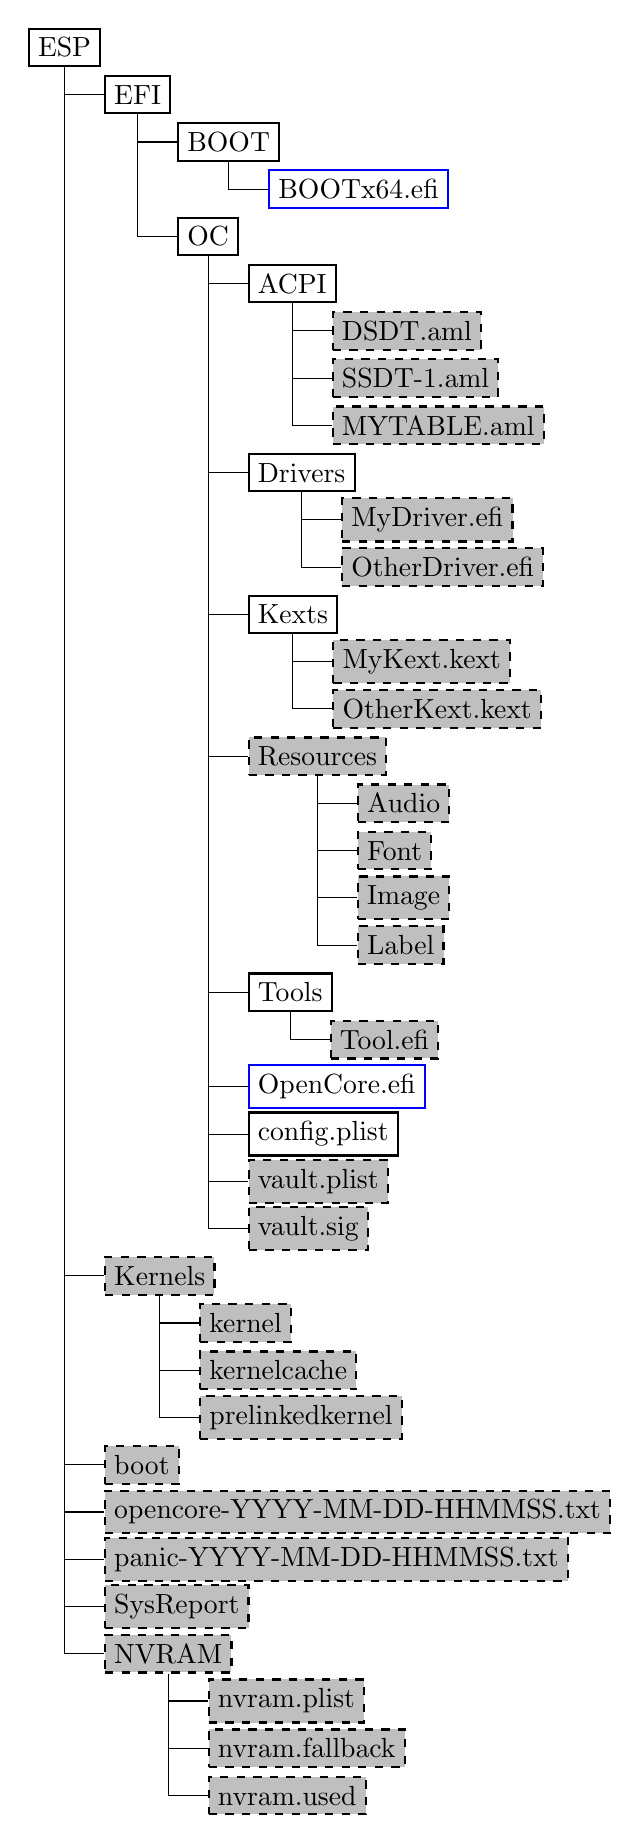
\begin{tikzpicture}[%
  grow via three points={one child at (0.5,-0.6) and
  two children at (0.5,-0.6) and (0.5,-1.2)},
  edge from parent path={(\tikzparentnode.south) |- (\tikzchildnode.west)}]
  \node {ESP}
    child { node {EFI}
      child { node {BOOT}
        child { node [selected] {BOOTx64.efi}}
      }
      child [missing] {}
      child { node {OC}
        child { node {ACPI}
          child { node [optional] {DSDT.aml}}
          child { node [optional] {SSDT-1.aml}}
          child { node [optional] {MYTABLE.aml}}
        }
        child [missing] {}
        child [missing] {}
        child [missing] {}
        child { node {Drivers}
          child { node [optional] {MyDriver.efi}}
          child { node [optional] {OtherDriver.efi}}
        }
        child [missing] {}
        child [missing] {}
        child { node {Kexts}
          child { node [optional] {MyKext.kext}}
          child { node [optional] {OtherKext.kext}}
        }
        child [missing] {}
        child [missing] {}
        child { node [optional] {Resources}
          child { node [optional] {Audio}}
          child { node [optional] {Font}}
          child { node [optional] {Image}}
          child { node [optional] {Label}}
        }
        child [missing] {}
        child [missing] {}
        child [missing] {}
        child [missing] {}
        child { node  {Tools}
          child { node [optional] {Tool.efi}}
        }
        child [missing] {}
        child { node [selected] {OpenCore.efi}}
        child { node {config.plist}}
        child { node [optional] {vault.plist}}
        child { node [optional] {vault.sig}}
      }
    }
    child [missing] {}
    child [missing] {}
    child [missing] {}
    child [missing] {}
    child [missing] {}
    child [missing] {}
    child [missing] {}
    child [missing] {}
    child [missing] {}
    child [missing] {}
    child [missing] {}
    child [missing] {}
    child [missing] {}
    child [missing] {}
    child [missing] {}
    child [missing] {}
    child [missing] {}
    child [missing] {}
    child [missing] {}
    child [missing] {}
    child [missing] {}
    child [missing] {}
    child [missing] {}
    child [missing] {}
    child { node [optional] {Kernels}
      child { node [optional] {kernel}}
      child { node [optional] {kernelcache}}
      child { node [optional] {prelinkedkernel}}
    }
    child [missing] {}
    child [missing] {}
    child [missing] {}
    child { node [optional] {boot}}
    child { node [optional] {opencore-YYYY-MM-DD-HHMMSS.txt}}
    child { node [optional] {panic-YYYY-MM-DD-HHMMSS.txt}}
    child { node [optional] {SysReport}}
    child { node [optional] {NVRAM}
      child { node [optional] {nvram.plist}}
      child { node [optional] {nvram.fallback}}
      child { node [optional] {nvram.used}}
    }
  ;
\end{tikzpicture}
\break
\label{fig:DS}
Figure 1. Directory Structure
\end{center}

When directory boot is used, the directory structure used should follow
the descriptions in the \hyperref[fig:DS]{Directory Structure} figure.
Available entries include:

\begin{itemize}
\tightlist
\item
  \texttt{BOOTx64.efi} or \texttt{BOOTIa32.efi} \\
  Initial bootstrap loaders, which load \texttt{OpenCore.efi}. \texttt{BOOTx64.efi}
  is loaded by the firmware by default consistent with the UEFI specification. However,
  it may also be renamed and put in a custom location to allow OpenCore coexist alongside
  operating systems, such as Windows, that use \texttt{BOOTx64.efi} files as their loaders.
  Refer to the \texttt{LauncherOption} property for details.
\item
  \texttt{boot} \\
  Duet bootstrap loader, which initialises the UEFI environment on legacy BIOS firmware
  and loads \texttt{OpenCore.efi} similarly to other bootstrap loaders. A modern Duet
  bootstrap loader will default to \texttt{OpenCore.efi} on the same partition when
  present.
\item
  \texttt{ACPI} \\
  Directory used for storing supplemental ACPI information
  for the \hyperref[acpi]{\texttt{ACPI}} section.
\item
  \texttt{Drivers} \\
  Directory used for storing supplemental \texttt{UEFI}
  drivers for \hyperref[uefi]{\texttt{UEFI}} section.
\item
  \texttt{Kexts} \\
  Directory used for storing supplemental kernel information
  for the \hyperref[kernel]{\texttt{Kernel}} section.
\item
  \texttt{Resources} \\
  Directory used for storing media resources such as audio files
  for screen reader support. Refer to the \hyperref[uefiaudioprops]{\texttt{UEFI Audio Properties}}
  section for details. This directory also contains image files
  for graphical user interface. Refer to the \hyperref[ueficanopy]{OpenCanopy} section for details.
\item
  \texttt{Tools} \\
  Directory used for storing supplemental tools.
\item
  \texttt{OpenCore.efi} \\
  Main booter application responsible for operating system loading. The directory
  \texttt{OpenCore.efi} resides in is called the \texttt{root directory}, which is
  set to \texttt{EFI\textbackslash OC} by default. When launching \texttt{OpenCore.efi}
  directly or through a custom launcher however, other directories containing
  \texttt{OpenCore.efi} files are also supported.
\item
  \texttt{config.plist} \\
  \texttt{OC Config}.
\item
  \texttt{vault.plist} \\
  Hashes for all files potentially loadable by \texttt{OC Config}.
\item
  \texttt{vault.sig} \\
  Signature for \texttt{vault.plist}.
\item
  \texttt{SysReport} \\
  Directory containing system reports generated by \texttt{SysReport} option.
\item
  \texttt{nvram.plist} \\
  OpenCore variable import file.
\item
  \texttt{nvram.fallback} \\
  OpenCore variable import fallback file.
\item
  \texttt{nvram.used} \\
  Renamed previous OpenCore variable import file after switch to fallback file.
\item
  \texttt{opencore-YYYY-MM-DD-HHMMSS.txt} \\
  OpenCore log file.
\item
  \texttt{panic-YYYY-MM-DD-HHMMSS.txt} \\
  Kernel panic log file.
\end{itemize}

\emph{Note}: It is not guaranteed that paths longer than
\texttt{OC\_STORAGE\_SAFE\_PATH\_MAX} (128 characters including
the \texttt{\\0}-terminator) will be accessible within OpenCore.

\subsection{Installation and Upgrade}\label{configuration-install}

To install OpenCore, replicate the
\hyperref[configuration-structure]{Configuration Structure} described
in the previous section in the EFI volume of a GPT partition. While
corresponding sections of this document provide some information
regarding external resources such as ACPI tables, UEFI drivers,
or kernel extensions (kexts), completeness of the matter is out of
the scope of this document. Information about kernel extensions may
be found in a separate
\href{https://github.com/acidanthera/OpenCorePkg/blob/master/Docs/Kexts.md}{Kext List}
document available in the OpenCore repository. Vaulting information is provided in
the \hyperref[miscsecurityprops]{Security Properties} section of this document.

The \texttt{OC\ config} file, as with any property list file, can be edited with
any text editor, such as nano or vim. However, specialised software
may provide a better experience. On macOS, the preferred GUI application is
\href{https://developer.apple.com/xcode}{Xcode}. The
\href{https://github.com/corpnewt/ProperTree}{ProperTree} editor
is a lightweight, cross-platform and open-source alternative.

It is strongly recommended to avoid configuration creation tools that are aware of the
internal configuration structure as this may result in invalid configurations (since the
structure gets constantly updated). If such tools are to be used despite this warning,
ensure that only stable versions of OpenCore explicitly supported by such tools are used.
In such cases, the use of open-source implementations with transparent binary generation
(such as \href{https://github.com/ic005k/QtOpenCoreConfig}{OCAT}) is encouraged, given
that other tools may contain malware. In addition, configurations created for a specific
hardware setup should never be used on different hardware setups.

For BIOS booting, a third-party UEFI environment provider is required and
\texttt{OpenDuetPkg} is one such UEFI environment provider for legacy systems.
To run OpenCore on such a legacy system, \texttt{OpenDuetPkg} can be installed
with a dedicated tool --- BootInstall (bundled with OpenCore).
\href{https://github.com/corpnewt/gibMacOS}{Third-party utilities} can be used
to perform this on systems other than macOS.

For upgrade purposes, refer to the \texttt{Differences.pdf} document which provides
information about changes to the configuration (as compared to the previous release)
as well as to the \texttt{Changelog.md} document (which contains a list of
modifications across all published updates).

\subsection{Contribution}\label{configuration-comp}

OpenCore can be compiled as a standard
\href{https://github.com/tianocore/tianocore.github.io/wiki/EDK-II}{EDK II}
package and requires the
\href{https://github.com/tianocore/tianocore.github.io/wiki/EDK-II#stable-tags}{EDK II Stable}
package. The currently supported EDK II release is hosted in
\href{https://github.com/acidanthera/audk}{acidanthera/audk}. Required patches
for this package can be found in the \texttt{Patches} directory.

When updating the LaTeX documentation (e.g. \texttt{Configuration.tex}) please
do \textit{not} rebuild the PDF files till merging to master happens. This avoids
unnecessary merge conflicts:
\begin{itemize}
\tightlist
\item External contributors using the pull-request approach should request
  the maintainers to handle the PDF rebuild in the pull-request message.
\item Internal contributors should rebuild the documentation at merge time
  in the same or in a separate commit. One can ask another maintainer to
  rebuild the documentation when lacking the necessary tools
  in the pull-request message.
\end{itemize}

The only officially supported toolchain is \texttt{XCODE5}. Other toolchains
might work but are neither supported nor recommended. Contributions of clean
patches are welcome. Please do follow
\href{https://github.com/tianocore/tianocore.github.io/wiki/Code-Style-C}{EDK II C Codestyle}.

To compile with \texttt{XCODE5}, besides \href{https://developer.apple.com/xcode}{Xcode},
users should also install \href{https://www.nasm.us}{NASM} and
\href{https://github.com/acidanthera/ocbuild/tree/master/external}{MTOC}.
The latest Xcode version is recommended for use despite the toolchain name.
An example command sequence is as follows:

\begin{lstlisting}[caption=Compilation Commands, label=compile, style=ocbash]
git clone --depth=1 https://github.com/acidanthera/audk UDK
cd UDK
git submodule update --init --recommend-shallow
rm -rf OpenCorePkg
git clone --depth=1 https://github.com/acidanthera/OpenCorePkg
. ./edksetup.sh
make -C BaseTools
build -a X64 -b RELEASE -t XCODE5 -p OpenCorePkg/OpenCorePkg.dsc
\end{lstlisting}

For IDE usage Xcode projects are available in the root of the repositories. Another
approach could be using \href{https://microsoft.github.io/language-server-protocol}{Language Server Protocols}. For example, \href{https://www.sublimetext.com}{Sublime Text} with
\href{https://lsp.sublimetext.io}{LSP for Sublime Text} plugin.
Add \texttt{compile\_flags.txt} file with similar content to the UDK root:

\begin{lstlisting}[caption=ECC Configuration, label=eccfile, style=ocbash]
-I/UefiPackages/MdePkg
-I/UefiPackages/MdePkg/Include
-I/UefiPackages/MdePkg/Include/X64
-I/UefiPackages/MdeModulePkg
-I/UefiPackages/MdeModulePkg/Include
-I/UefiPackages/MdeModulePkg/Include/X64
-I/UefiPackages/OpenCorePkg/Include/AMI
-I/UefiPackages/OpenCorePkg/Include/Acidanthera
-I/UefiPackages/OpenCorePkg/Include/Apple
-I/UefiPackages/OpenCorePkg/Include/Apple/X64
-I/UefiPackages/OpenCorePkg/Include/Duet
-I/UefiPackages/OpenCorePkg/Include/Generic
-I/UefiPackages/OpenCorePkg/Include/Intel
-I/UefiPackages/OpenCorePkg/Include/Microsoft
-I/UefiPackages/OpenCorePkg/Include/Nvidia
-I/UefiPackages/OpenCorePkg/Include/VMware
-I/UefiPackages/OvmfPkg/Include
-I/UefiPackages/ShellPkg/Include
-I/UefiPackages/UefiCpuPkg/Include
-IInclude
-include
/UefiPackages/MdePkg/Include/Uefi.h
-fshort-wchar
-Wall
-Wextra
-Wno-unused-parameter
-Wno-missing-braces
-Wno-missing-field-initializers
-Wno-tautological-compare
-Wno-sign-compare
-Wno-varargs
-Wno-unused-const-variable
-DOC_TARGET_NOOPT=1
-DNO_MSABI_VA_FUNCS=1
\end{lstlisting}

\emph{Note}: \texttt{/UefiPackages} in the sample file denotes an absolute path.

\textbf{Warning}: Tool developers modifying \texttt{config.plist} or any other OpenCore
files must ensure that their tools check the \texttt{opencore-version} NVRAM variable
(see the \hyperref[miscdebugprops]{Debug Properties} section below) and warn users
if the version listed is unsupported or prerelease. The OpenCore configuration may change
across releases and such tools shall ensure that they carefully follow this document. Failure
to do so may result in such tools being considered to be malware and blocked by any means.

\subsection{Coding conventions}\label{configuration-conv}

As with any other project, we have conventions that we follow during development.
All third-party contributors are advised to adhere to the conventions listed below
before submitting patches. To minimise abortive work and the potential rejection of
submissions, third-party contributors should initially raise issues to the
\href{https://github.com/acidanthera/bugtracker}{Acidanthera Bugtracker}
for feedback before submitting patches.

\textbf{Organisation}. The codebase is contained in the \texttt{OpenCorePkg} repository,
which is the primary EDK II package.
\begin{itemize}
\tightlist
\item Whenever changes are required in multiple repositories, separate pull requests should
be sent to each.
\item Committing the changes should happen firstly to dependent repositories, secondly to
primary repositories to avoid automatic build errors.
\item Each unique commit should compile with \texttt{XCODE5} and preferably with other
toolchains. In the majority of the cases it can be checked by accessing the
\href{https://travis-ci.com/acidanthera}{CI interface}. Ensuring that static analysis finds
no warnings is preferred.
\item External pull requests and tagged commits must be validated. That said, commits in
master may build but may not necessarily work.
\item Internal branches should be named as follows: \texttt{author-name-date}, e.g.
\texttt{vit9696-ballooning-20191026}.
\item Commit messages should be prefixed with the primary module (e.g. library or code module) the
changes were made in. For example, \texttt{OcGuardLib: Add OC\_ALIGNED macro}. For non-library changes
\texttt{Docs} or \texttt{Build} prefixes are used.
\end{itemize}

\textbf{Design}. The codebase is written in a subset of freestanding C11 (C17) supported by
most modern toolchains used by EDK II. Applying common software development practices or requesting
clarification is recommended if any particular case is not discussed below.
\begin{itemize}
\tightlist
\item Never rely on undefined behaviour and try to avoid implementation defined behaviour unless
explicitly covered below (feel free to create an issue when a relevant case is not present).
\item Use \texttt{OcGuardLib} to ensure safe integral arithmetics avoiding overflows. Unsigned
wraparound should be relied on with care and reduced to the necessary amount.
\item Check pointers for correct alignment with \texttt{OcGuardLib} and do not rely on the architecture
being able to dereference unaligned pointers.
\item Use flexible array members instead of zero-length or one-length arrays where necessary.
\item Use static assertions (\texttt{STATIC\_ASSERT}) for type and value assumptions, and runtime
assertions (\texttt{ASSERT}) for precondition and invariant sanity checking. Do not use runtime
assertions to check for errors as they should never alter control flow and potentially be excluded.
\item Assume \texttt{UINT32}/\texttt{INT32} to be \texttt{int}-sized and use \texttt{\%u},
\texttt{\%d}, and \texttt{\%x} to print them.
\item Assume \texttt{UINTN}/\texttt{INTN} to be of unspecified size, and cast them to
\texttt{UINT64}/\texttt{INT64} for printing with \texttt{\%Lu}, \texttt{\%Ld} and so on as normal.
\item Do not rely on integer promotions for numeric literals. Use explicit casts when the type is
implementation-dependent or suffixes when type size is known. Assume \texttt{U} for \texttt{UINT32}
and \texttt{ULL} for \texttt{UINT64}.
\item Do ensure unsigned arithmetics especially in bitwise maths, shifts in particular.
\item \texttt{sizeof} operator should take variables instead of types where possible to be error prone.
Use \texttt{ARRAY\_SIZE} to obtain array size in elements. Use \texttt{L\_STR\_LEN} and
\texttt{L\_STR\_SIZE} macros from \texttt{OcStringLib} to obtain string literal sizes to ensure compiler
optimisation.
\item Do not use \texttt{goto} keyword. Prefer early \texttt{return}, \texttt{break}, or \texttt{continue}
after failing to pass error checking instead of nesting conditionals.
\item Use \texttt{EFIAPI}, force UEFI calling convention, only in protocols, external callbacks between
modules, and functions with variadic arguments.
\item Provide inline documentation to every added function, at least describing its inputs, outputs,
precondition, postcondition, and giving a brief description.
\item Do not use \texttt{RETURN\_STATUS}. Assume \texttt{EFI\_STATUS} to be a matching superset that is
to be always used when \texttt{BOOLEAN} is not enough.
\item Security violations should halt the system or cause a forced reboot.
\end{itemize}

\textbf{Codestyle}. The codebase follows the
\href{https://github.com/tianocore/tianocore.github.io/wiki/Code-Style-C}{EDK II codestyle}
with a few changes and clarifications.
\begin{itemize}
\tightlist
\item Write inline documentation for the functions and variables only once: in headers, where a header prototype
is available, and inline for \texttt{static} variables and functions.
\item Use line length of 120 characters or less, preferably 100 characters.
\item Use spaces after casts, e.g. \texttt{(VOID *)(UINTN) Variable}.
\item Use two spaces to indent function arguments when splitting lines.
\item Prefix public functions with either \texttt{Oc} or another distinct name.
\item Do not prefix private \texttt{static} functions, but prefix private \texttt{non-static} functions with \texttt{Internal}.
\item Use SPDX license headers as shown in
\href{https://github.com/acidanthera/bugtracker/issues/483}{acidanthera/bugtracker\#483}.
\end{itemize}

\subsection{Debugging}\label{configuration-debug}

The codebase incorporates EDK II debugging and few custom features to improve the experience.
\begin{itemize}
\tightlist
\item Use module prefixes, 2-5 letters followed by a colon (\texttt{:}), for debug messages. For \texttt{OpenCorePkg}
use \texttt{OC:}, for libraries and drivers use their own unique prefixes.
\item Do not use dots (\texttt{.}) in the end of debug messages and separate \texttt{EFI\_STATUS}, printed by
\texttt{\%r}, with a hyphen (e.g. \texttt{OCRAM: Allocation of \%u bytes failed - \%r\textbackslash n}).
\item Use \texttt{DEBUG\_CODE\_BEGIN ()} and \texttt{DEBUG\_CODE\_END ()} constructions to guard debug checks
that may potentially reduce the performance of release builds and are otherwise unnecessary.
\item Use \texttt{DEBUG} macro to print debug messages during normal functioning, and \texttt{RUNTIME\_DEBUG} for
debugging after \texttt{EXIT\_BOOT\_SERVICES}.
\item Use \texttt{DEBUG\_VERBOSE} debug level to leave debug messages for future debugging of the code, which
are currently not necessary. By default \texttt{DEBUG\_VERBOSE} messages are ignored even in \texttt{DEBUG} builds.
\item Use \texttt{DEBUG\_INFO} debug level for all non critical messages (including errors)
and \texttt{DEBUG\_BULK\_INFO}
for extensive messages that should not appear in NVRAM log that is heavily limited in size.
These messages are ignored in \texttt{RELEASE} builds.
\item Use \texttt{DEBUG\_ERROR} to print critical human visible messages that may potentially halt the boot process,
and \texttt{DEBUG\_WARN} for all other human visible errors, \texttt{RELEASE} builds included.
\end{itemize}

The \href{https://git-scm.com/docs/git-bisect}{\texttt{git-bisect}} functionality may be useful when trying
to find problematic changes. Unofficial sources of \texttt{per-commit} OpenCore binary builds,
such as \href{https://dortania.github.io/builds}{Dortania}, may also be useful.

\section{ACPI}\label{acpi}

\subsection{Introduction}\label{acpiintro}

ACPI (Advanced Configuration and Power Interface) is an open standard to
discover and configure computer hardware.
The \href{https://uefi.org/specifications}{ACPI specification} defines
standard tables (e.g.~\texttt{DSDT}, \texttt{SSDT}, \texttt{FACS}, \texttt{DMAR})
and various methods (e.g. \texttt{\_DSM}, \texttt{\_PRW}) for implementation.
Modern hardware needs few changes to maintain ACPI compatibility and some
options for such changes are provided as part of OpenCore.

To compile and disassemble ACPI tables, the \href{https://github.com/acpica/acpica}{iASL compiler}
developed by \href{https://www.acpica.org}{ACPICA} can be used. A GUI front-end to iASL compiler
can be downloaded from \href{https://github.com/acidanthera/MaciASL/releases}{Acidanthera/MaciASL}.

ACPI changes apply globally (to every operating system) with the following effective order:

\begin{itemize}
\tightlist
\item \texttt{Delete} is processed.
\item \texttt{Quirks} are processed.
\item \texttt{Patch} is processed.
\item \texttt{Add} is processed.
\end{itemize}

\emph{Note}: \texttt{RebaseRegions} and \texttt{SyncTableIds} quirks are special and are processed after all other ACPI changes since they can only be applied on the final ACPI configuration including all the patches and added tables.

Applying the changes globally resolves the problems of incorrect operating system
detection (consistent with the ACPI specification, not possible before the operating
system boots), operating system chainloading, and difficult ACPI debugging. Hence,
more attention may be required when writing changes to \texttt{\_OSI}.

Applying the patches early makes it possible to write so called ``proxy'' patches,
where the original method is patched in the original table and is implemented in
the patched table.

There are several sources of ACPI tables and workarounds. Commonly used
ACPI tables are provided with OpenCore, VirtualSMC, VoodooPS2, and WhateverGreen
releases. Besides those, several third-party instructions may be found on
the AppleLife \href{https://applelife.ru/forums/xakintosh.67}{Laboratory}
and \href{https://applelife.ru/forums/dsdt.129}{DSDT} subforums
(e.g. \href{https://applelife.ru/posts/498967}{Battery register splitting} guide).
A slightly more user-friendly explanation of some tables included with OpenCore
can also be found in \href{https://dortania.github.io}{Dortania}'s
\href{https://dortania.github.io/Getting-Started-With-ACPI}{Getting started with ACPI} guide.
For more exotic cases, there are several alternatives such as
\href{https://github.com/daliansky}{daliansky}'s
\href{https://github.com/daliansky/OC-little}{ACPI sample collection}
(\href{https://github.com/5T33Z0/OC-Little-Translated}{English Translation by 5T33Z0 et al}).
Please note however, that suggested solutions from third parties may be outdated or may contain errors.

\subsection{Properties}\label{acpiprops}

\begin{enumerate}
\item
  \texttt{Add}\\
  \textbf{Type}: \texttt{plist\ array}\\
  \textbf{Failsafe}: Empty\\
  \textbf{Description}: Load selected tables from the \texttt{OC/ACPI}
  directory.

  To be filled with \texttt{plist\ dict} values, describing each add entry.
  Refer to the \hyperref[acpipropsadd]{Add Properties} section below for details.

\item
  \texttt{Delete}\\
  \textbf{Type}: \texttt{plist\ array}\\
  \textbf{Failsafe}: Empty\\
  \textbf{Description}: Remove selected tables from the ACPI stack.

  To be filled with \texttt{plist\ dict} values, describing each delete entry.
  Refer to the \hyperref[acpipropsdelete]{Delete Properties} section below for details.

\item
  \texttt{Patch}\\
  \textbf{Type}: \texttt{plist\ array}\\
  \textbf{Failsafe}: Empty\\
  \textbf{Description}: Perform binary patches in ACPI tables before
  table addition or removal.

  To be filled with \texttt{plist\ dictionary} values describing each patch entry.
  Refer to the \hyperref[acpipropspatch]{Patch Properties} section below for details.

\item
  \texttt{Quirks}\\
  \textbf{Type}: \texttt{plist\ dict}\\
  \textbf{Description}: Apply individual ACPI quirks described
  in the \hyperref[acpipropsquirks]{Quirks Properties} section below.

\end{enumerate}

\subsection{Add Properties}\label{acpipropsadd}

\begin{enumerate}
\item
  \texttt{Comment}\\
  \textbf{Type}: \texttt{plist\ string}\\
  \textbf{Failsafe}: Empty\\
  \textbf{Description}: Arbitrary ASCII string used to provide human readable
  reference for the entry. Whether this value is used is implementation defined.

\item
  \texttt{Enabled}\\
  \textbf{Type}: \texttt{plist\ boolean}\\
  \textbf{Failsafe}: \texttt{false}\\
  \textbf{Description}: Set to \texttt{true} to add this ACPI table.

\item
  \texttt{Path}\\
  \textbf{Type}: \texttt{plist\ string}\\
  \textbf{Failsafe}: Empty\\
  \textbf{Description}: File paths meant to be loaded as ACPI tables.
  Example values include \texttt{DSDT.aml}, \texttt{SubDir/SSDT-8.aml},
  \texttt{SSDT-USBX.aml}, etc.

  The ACPI table load order follows the item order in the array. ACPI tables
  are loaded from the \texttt{OC/ACPI} directory.

  \textbf{Note}: All tables apart from tables with a \texttt{DSDT} table identifier
  (determined by parsing data, not by filename) insert new tables into the ACPI stack.
  \texttt{DSDT} tables perform a replacement of DSDT tables instead.

\end{enumerate}

\subsection{Delete Properties}\label{acpipropsdelete}

\begin{enumerate}
\item
  \texttt{All}\\
  \textbf{Type}: \texttt{plist\ boolean}\\
  \textbf{Failsafe}: \texttt{false} (Only delete the first matched table)\\
  \textbf{Description}: Set to \texttt{true} to delete all ACPI tables matching the
  condition.

\item
  \texttt{Comment}\\
  \textbf{Type}: \texttt{plist\ string}\\
  \textbf{Failsafe}: Empty\\
  \textbf{Description}: Arbitrary ASCII string used to provide human readable
  reference for the entry. Whether this value is used is implementation defined.

\item
  \texttt{Enabled}\\
  \textbf{Type}: \texttt{plist\ boolean}\\
  \textbf{Failsafe}: \texttt{false}\\
  \textbf{Description}: Set to \texttt{true} to remove this ACPI table.

\item
  \texttt{OemTableId}\\
  \textbf{Type}: \texttt{plist\ data}, 8 bytes\\
  \textbf{Failsafe}: All zero (Match any table OEM ID)\\
  \textbf{Description}: Match table OEM ID equal to this value.

\item
  \texttt{TableLength}\\
  \textbf{Type}: \texttt{plist\ integer}\\
  \textbf{Failsafe}: \texttt{0} (Match any table size)\\
  \textbf{Description}: Match table size equal to this value.

\item
  \texttt{TableSignature}\\
  \textbf{Type}: \texttt{plist\ data}, 4 bytes\\
  \textbf{Failsafe}: All zero (Match any table signature)\\
  \textbf{Description}: Match table signature equal to this value.

  \emph{Note}: Do not use table signatures when the sequence
  must be replaced in multiple places. This is particularly relevant
  when performing different types of renames.

\end{enumerate}

\subsection{Patch Properties}\label{acpipropspatch}

\begin{enumerate}

\item
  \texttt{Base}\\
  \textbf{Type}: \texttt{plist\ string}\\
  \textbf{Failsafe}: Empty (Ignored)\\
  \textbf{Description}: Selects ACPI path base for patch lookup (or immediate
  replacement) by obtaining the offset to the provided path.

  Only fully-qualified absolute paths are supported (e.g. \texttt{\textbackslash \_SB.PCI0.LPCB.HPET}).
  Currently supported object types are: \texttt{Device}, \texttt{Field}, \texttt{Method}.

  \emph{Note}: Use with care, not all OEM tables can be parsed. Use \texttt{ACPIe}
  utility to debug. \texttt{ACPIe} compiled  with \texttt{DEBUG=1 make} command
  produces helpful ACPI lookup tracing.

\item
  \texttt{BaseSkip}\\
  \textbf{Type}: \texttt{plist\ integer}\\
  \textbf{Failsafe}: \texttt{0} (Do not skip any occurrences)\\
  \textbf{Description}: Number of found \texttt{Base} occurrences to skip before
  finds and replacements are applied.

\item
  \texttt{Comment}\\
  \textbf{Type}: \texttt{plist\ string}\\
  \textbf{Failsafe}: Empty\\
  \textbf{Description}: Arbitrary ASCII string used to provide human readable
  reference for the entry. Whether this value is used is implementation defined.

\item
  \texttt{Count}\\
  \textbf{Type}: \texttt{plist\ integer}\\
  \textbf{Failsafe}: \texttt{0} (Apply patch to all occurrences found)\\
  \textbf{Description}: Number of occurrences to patch.

\item
  \texttt{Enabled}\\
  \textbf{Type}: \texttt{plist\ boolean}\\
  \textbf{Failsafe}: \texttt{false}\\
  \textbf{Description}: Set to \texttt{true} to apply this ACPI patch.

\item
  \texttt{Find}\\
  \textbf{Type}: \texttt{plist\ data}\\
  \textbf{Failsafe}: Empty\\
  \textbf{Description}: Data to find. Must be equal to \texttt{Replace} in size if set.

  \emph{Note}: Can be empty, when \texttt{Base} is specified, immediate replacement
  after \texttt{Base} lookup happens in this case.

\item
  \texttt{Limit}\\
  \textbf{Type}: \texttt{plist\ integer}\\
  \textbf{Failsafe}: \texttt{0} (Search entire ACPI table)\\
  \textbf{Description}: Maximum number of bytes to search for.

\item
  \texttt{Mask}\\
  \textbf{Type}: \texttt{plist\ data}\\
  \textbf{Failsafe}: Empty (Ignored)\\
  \textbf{Description}: Data bitwise mask used during find comparison.
  Allows fuzzy search by ignoring not masked (set to zero) bits.
  Must be equal to \texttt{Replace} in size if set.

\item
  \texttt{OemTableId}\\
  \textbf{Type}: \texttt{plist\ data}, 8 bytes\\
  \textbf{Failsafe}: All zero (Match any table OEM ID)\\
  \textbf{Description}: Match table OEM ID equal to this value.

\item
  \texttt{Replace}\\
  \textbf{Type}: \texttt{plist\ data}\\
  \textbf{Failsafe}: Empty\\
  \textbf{Description}: Replacement data of one or more bytes.

\item
  \texttt{ReplaceMask}\\
  \textbf{Type}: \texttt{plist\ data}\\
  \textbf{Failsafe}: Empty (Ignored)\\
  \textbf{Description}: Data bitwise mask used during replacement.
  Allows fuzzy replacement by updating masked (set to non-zero) bits.
  Must be equal to \texttt{Replace} in size if set.

\item
  \texttt{Skip}\\
  \textbf{Type}: \texttt{plist\ integer}\\
  \textbf{Failsafe}: \texttt{0} (Do not skip any occurrences)\\
  \textbf{Description}: Number of found occurrences to skip before
  replacements are applied.

\item
  \texttt{TableLength}\\
  \textbf{Type}: \texttt{plist\ integer}\\
  \textbf{Failsafe}: \texttt{0} (Match any table size)\\
  \textbf{Description}: Match table size equal to this value.

\item
  \texttt{TableSignature}\\
  \textbf{Type}: \texttt{plist\ data}, 4 bytes\\
  \textbf{Failsafe}: All zero (Match any table signature)\\
  \textbf{Description}: Match table signature equal to this value.

\end{enumerate}

In most cases, ACPI patches are not useful and are harmful:

\begin{itemize}
\item
  Avoid renaming devices with ACPI patches. This may fail or perform
  improper renaming of unrelated devices (e.g. \texttt{EC} and
  \texttt{EC0}), be unnecessary, or even fail to rename devices in certain tables. For
  ACPI consistency it is much safer to rename devices at the I/O Registry
  level, as done by
  \href{https://github.com/acidanthera/WhateverGreen}{WhateverGreen}.
\item
  Avoid patching \texttt{\_OSI} to support a higher feature set level
  whenever possible. While this enables a number of workarounds on APTIO
  firmware, it typically results in a need for additional patches. These are
  not usually needed on modern firmware and smaller patches work well on
  firmware that does. However, laptop vendors often rely on this method to
  determine the availability of functions such as modern I2C input support, thermal
  adjustment and custom feature additions.
\item
  Avoid patching embedded controller event \texttt{\_Qxx} just to enable
  brightness keys. The conventional process to find these keys typically involves
  significant modifications to DSDT and SSDT files and in addition, the debug kext
  is not stable on newer systems. Please use the built-in brightness key discovery in
  \href{https://github.com/acidanthera/BrightnessKeys}{BrightnessKeys} instead.
\item
  Avoid making ad hoc changes such as renaming \texttt{\_PRW} or \texttt{\_DSM}
  whenever possible.
\end{itemize}

Some cases where patching is actually useful include:

\begin{itemize}
\item
  Refreshing \texttt{HPET} (or another device) method header to avoid
  compatibility checks by \texttt{\_OSI} on legacy hardware. \texttt{\_STA}
  method with \texttt{if ((OSFL () == Zero)) \{ If (HPTE)  ...  Return (Zero)}
  content may be forced to always return 0xF by replacing
  \texttt{A0 10 93 4F 53 46 4C 00} with \texttt{A4 0A 0F A3 A3 A3 A3 A3}.
\item
  To provide a custom method implementation within an SSDT, to inject
  shutdown fixes on certain computers for instance, the original method can
  be replaced with a dummy name by patching \texttt{\_PTS} with \texttt{ZPTS}
  and adding a callback to the original method.
\end{itemize}

The Tianocore \href{https://github.com/acidanthera/audk/blob/master/MdePkg/Include/IndustryStandard/AcpiAml.h}{AcpiAml.h} source file may help with better understanding ACPI opcodes.

\emph{Note}: Patches of different \texttt{Find} and \texttt{Replace} lengths
are unsupported as they may corrupt ACPI tables and make the system unstable
due to area relocation. If such changes are needed, the utilisation of ``proxy''
patching or the padding of \texttt{NOP} to the remaining area could be considered.

\subsection{Quirks Properties}\label{acpipropsquirks}

\begin{enumerate}

\item
  \texttt{FadtEnableReset}\\
  \textbf{Type}: \texttt{plist\ boolean}\\
  \textbf{Failsafe}: \texttt{false}\\
  \textbf{Description}: Provide reset register and flag in FADT table to enable
  reboot and shutdown.

  Mainly required on legacy hardware and a few newer laptops.
  Can also fix power-button shortcuts. Not recommended unless required.

\item
  \texttt{NormalizeHeaders}\\
  \textbf{Type}: \texttt{plist\ boolean}\\
  \textbf{Failsafe}: \texttt{false}\\
  \textbf{Description}: Cleanup ACPI header fields to workaround macOS
  ACPI implementation flaws that result in boot crashes. Reference:
  \href{https://alextjam.es/debugging-appleacpiplatform/}{Debugging
  AppleACPIPlatform on 10.13} by Alex James (also known as theracermaster).
  The issue was fixed in macOS Mojave (10.14).

\item
  \texttt{RebaseRegions}\\
  \textbf{Type}: \texttt{plist\ boolean}\\
  \textbf{Failsafe}: \texttt{false}\\
  \textbf{Description}: Attempt to heuristically relocate ACPI memory
  regions. Not recommended.

  ACPI tables are often generated dynamically by the underlying firmware
  implementation. Among the position-independent code, ACPI tables may
  contain the physical addresses of MMIO areas used for device
  configuration, typically grouped by region (e.g.
  \texttt{OperationRegion}). Changing firmware settings or hardware
  configuration, upgrading or patching the firmware inevitably leads to
  changes in dynamically generated ACPI code, which sometimes results in
  the shift of the addresses in the aforementioned \texttt{OperationRegion}
  constructions.

  For this reason, the application of modifications to ACPI tables is extremely
  risky. The best approach is to make as few changes as possible to ACPI tables
  and to avoid replacing any tables, particularly DSDT tables. When this cannot be
  avoided, ensure that any custom DSDT tables are based on the most recent DSDT
  tables or attempt to remove reads and writes for the affected areas.

  When nothing else helps, this option could be tried to avoid stalls at
  \texttt{PCI\ Configuration\ Begin} phase of macOS booting by attempting to fix
  the ACPI addresses. It is not a magic bullet however, and only works with the
  most typical cases. Do not use unless absolutely required as it can have the
  opposite effect on certain platforms and result in boot failures.

\item
  \texttt{ResetHwSig}\\
  \textbf{Type}: \texttt{plist\ boolean}\\
  \textbf{Failsafe}: \texttt{false}\\
  \textbf{Description}: Reset \texttt{FACS} table \texttt{HardwareSignature}
  value to \texttt{0}.

  This works around firmware that fail to maintain hardware signature across
  the reboots and cause issues with waking from hibernation.

\item
  \texttt{ResetLogoStatus}\\
  \textbf{Type}: \texttt{plist\ boolean}\\
  \textbf{Failsafe}: \texttt{false}\\
  \textbf{Description}: Reset \texttt{BGRT} table \texttt{Displayed}
  status field to \texttt{false}.

  This works around firmware that provide a \texttt{BGRT} table but
  fail to handle screen updates afterwards.

\item
  \texttt{SyncTableIds}\\
  \textbf{Type}: \texttt{plist\ boolean}\\
  \textbf{Failsafe}: \texttt{false}\\
  \textbf{Description}: Sync table identifiers with the \texttt{SLIC} table.

  This works around patched tables becoming incompatible with the \texttt{SLIC}
  table causing licensing issues in older Windows operating systems.

\end{enumerate}


\section{Booter}\label{booter}

\subsection{Introduction}\label{booterintro}

This section allows the application of different types of UEFI modifications to
operating system bootloaders, primarily the Apple bootloader (\texttt{boot.efi}).
The modifications currently provide various patches and environment alterations for
different firmware types. Some of these features were originally implemented as part
of \href{https://github.com/acidanthera/AptioFixPkg}{\text{AptioMemoryFix.efi}},
which is no longer maintained. Refer to the \hyperref[troubleshootingtricks]{Tips and Tricks}
section for instructions on migration.

Booter changes apply with the following effective order:
\begin{itemize}
\tightlist
\item \texttt{Quirks} are processed.
\item \texttt{Patch} is processed.
\end{itemize}

If this is used for the first time on customised firmware, the following requirements
should be met before starting:

\begin{itemize}
\tightlist
\item Most up-to-date UEFI firmware (check the motherboard vendor website).
\item \texttt{Fast Boot} and \texttt{Hardware Fast Boot} disabled in firmware
  settings if present.
\item \texttt{Above 4G Decoding} or similar enabled in firmware
  settings if present. Note that on some motherboards, notably the ASUS WS-X299-PRO, this
  option results in adverse effects and must be disabled. While no other motherboards
  with the same issue are known, this option should be checked first whenever erratic boot
  failures are encountered.
\item \texttt{DisableIoMapper} quirk enabled, or \texttt{VT-d} disabled in
  firmware settings if present, or ACPI DMAR table deleted.
\item \textbf{No} `slide` boot argument present in NVRAM or anywhere else.
  It is not necessary unless the system cannot be booted at all or
  \texttt{No slide values are usable! Use custom slide!} message can be seen in the log.
\item \texttt{CFG Lock} (MSR \texttt{0xE2} write protection) disabled in
  firmware settings if present. Refer to the \hyperref[kernelpropsquirks]{ControlMsrE2}
  notes for details.
\item \texttt{CSM} (Compatibility Support Module) disabled in firmware settings
  if present. On NVIDIA 6xx/AMD 2xx or older, GOP ROM may have to be flashed first. Use
  \href{https://www.win-raid.com/t892f16-AMD-and-Nvidia-GOP-update-No-requests-DIY.html}{GopUpdate}
  (see the second post) or \href{http://www.insanelymac.com/forum/topic/299614-asus-eah6450-video-bios-uefi-gop-upgrade-and-gop-uefi-binary-in-efi-for-many-ati-cards/page-1#entry2042163}{AMD UEFI GOP MAKER}
  in case of any potential confusion.
\item \texttt{EHCI/XHCI Hand-off} enabled in firmware settings \texttt{only} if boot
  stalls unless USB devices are disconnected.
\item \texttt{VT-x}, \texttt{Hyper Threading}, \texttt{Execute Disable Bit} enabled
  in firmware settings if present.
\item While it may not be required, sometimes
  \texttt{Thunderbolt support}, \texttt{Intel SGX}, and \texttt{Intel Platform Trust}
  may have to be disabled in firmware settings present.
\end{itemize}

When debugging sleep issues, Power Nap and automatic power off (which appear to sometimes cause
wake to black screen or boot loop issues on older platforms) may be temporarily disabled.
The specific issues may vary, but ACPI tables should typically be looked at first.

Here is an example of a defect found on some
\href{http://www.insanelymac.com/forum/topic/329624-need-cmos-reset-after-sleep-only-after-login/#entry2534645}{Z68 motherboards}.
To turn Power Nap and the others off, run the following commands in Terminal:
\begin{lstlisting}[label=powernap, style=ocbash]
sudo pmset autopoweroff 0
sudo pmset powernap 0
sudo pmset standby 0
\end{lstlisting}

\emph{Note}: These settings may be reset by hardware changes and in certain other circumstances.
To view their current state, use the \texttt{pmset -g} command in Terminal.

\subsection{Properties}\label{booterprops}

\begin{enumerate}

\item
  \texttt{MmioWhitelist}\\
  \textbf{Type}: \texttt{plist\ array}\\
  \textbf{Failsafe}: Empty\\
  \textbf{Description}: To be filled with \texttt{plist\ dict} values,
  describing addresses critical for particular firmware functioning when
  \texttt{DevirtualiseMmio} quirk is in use.
  Refer to the \hyperref[booterpropsmmio]{MmioWhitelist Properties} section below for details.

\item
  \texttt{Patch}\\
  \textbf{Type}: \texttt{plist\ array}\\
  \textbf{Failsafe}: Empty\\
  \textbf{Description}: Perform binary patches in booter.

  To be filled with \texttt{plist\ dictionary} values, describing each
  patch. Refer to the \hyperref[booterpropspatch]{Patch Properties} section below for details.

\item
  \texttt{Quirks}\\
  \textbf{Type}: \texttt{plist\ dict}\\
  \textbf{Description}: Apply individual booter quirks described
  in the \hyperref[booterpropsquirks]{Quirks Properties} section below.

\end{enumerate}

\subsection{MmioWhitelist Properties}\label{booterpropsmmio}

\begin{enumerate}

\item
  \texttt{Address}\\
  \textbf{Type}: \texttt{plist\ integer}\\
  \textbf{Failsafe}: \texttt{0}\\
  \textbf{Description}: Exceptional MMIO address, which memory descriptor should be left
  virtualised (unchanged) by \texttt{DevirtualiseMmio}. This means that the firmware will
  be able to directly communicate with this memory region during operating system functioning,
  because the region this value is in will be assigned a virtual address.

  The addresses written here must be part of the memory map, have \texttt{EfiMemoryMappedIO}
  type and \texttt{EFI\_MEMORY\_RUNTIME} attribute (highest bit) set. The debug log can be used
  to find the list of the candidates.

\item
  \texttt{Comment}\\
  \textbf{Type}: \texttt{plist\ string}\\
  \textbf{Failsafe}: Empty\\
  \textbf{Description}: Arbitrary ASCII string used to provide human readable
  reference for the entry. Whether this value is used is implementation defined.

\item
  \texttt{Enabled}\\
  \textbf{Type}: \texttt{plist\ boolean}\\
  \textbf{Failsafe}: \texttt{false}\\
  \textbf{Description}: Exclude MMIO address from the devirtualisation procedure.

\end{enumerate}

\subsection{Patch Properties}\label{booterpropspatch}

\begin{enumerate}
\item
  \texttt{Arch}\\
  \textbf{Type}: \texttt{plist\ string}\\
  \textbf{Failsafe}: \texttt{Any} (Apply to any supported architecture)\\
  \textbf{Description}: Booter patch architecture (\texttt{i386}, \texttt{x86\_64}).

\item
  \texttt{Comment}\\
  \textbf{Type}: \texttt{plist\ string}\\
  \textbf{Failsafe}: Empty\\
  \textbf{Description}: Arbitrary ASCII string used to provide human readable
  reference for the entry. Whether this value is used is implementation defined.

\item
  \texttt{Count}\\
  \textbf{Type}: \texttt{plist\ integer}\\
  \textbf{Failsafe}: \texttt{0} (Apply to all occurrences found)\\
  \textbf{Description}: Number of patch occurrences to apply.

\item
  \texttt{Enabled}\\
  \textbf{Type}: \texttt{plist\ boolean}\\
  \textbf{Failsafe}: \texttt{false}\\
  \textbf{Description}: Set to \texttt{true} to activate this booter patch.

\item
  \texttt{Find}\\
  \textbf{Type}: \texttt{plist\ data}\\
  \textbf{Failsafe}: Empty\\
  \textbf{Description}: Data to find. Must be equal to \texttt{Replace} in size if set.

\item
  \texttt{Identifier}\\
  \textbf{Type}: \texttt{plist\ string}\\
  \textbf{Failsafe}:  \texttt{Any} (Match any booter)\\
  \textbf{Description}: \texttt{Apple} for macOS booter (typically \texttt{boot.efi});
  or a name with a suffix, such as \texttt{bootmgfw.efi}, for a specific booter.

\item
  \texttt{Limit}\\
  \textbf{Type}: \texttt{plist\ integer}\\
  \textbf{Failsafe}: \texttt{0} (Search the entire booter)\\
  \textbf{Description}: Maximum number of bytes to search for.

\item
  \texttt{Mask}\\
  \textbf{Type}: \texttt{plist\ data}\\
  \textbf{Failsafe}: Empty (Ignored)\\
  \textbf{Description}: Data bitwise mask used during find comparison.
  Allows fuzzy search by ignoring not masked (set to zero) bits.
  Must be equal to \texttt{Find} in size if set.

\item
  \texttt{Replace}\\
  \textbf{Type}: \texttt{plist\ data}\\
  \textbf{Failsafe}: Empty\\
  \textbf{Description}: Replacement data of one or more bytes.

\item
  \texttt{ReplaceMask}\\
  \textbf{Type}: \texttt{plist\ data}\\
  \textbf{Failsafe}: Empty (Ignored)\\
  \textbf{Description}: Data bitwise mask used during replacement.
  Allows fuzzy replacement by updating masked (set to non-zero) bits.
  Must be equal to \texttt{Replace} in size if set.

\item
  \texttt{Skip}\\
  \textbf{Type}: \texttt{plist\ integer}\\
  \textbf{Failsafe}: \texttt{0} (Do not skip any occurrences)\\
  \textbf{Description}: Number of found occurrences to skip before
  replacements are applied.

\end{enumerate}

\subsection{Quirks Properties}\label{booterpropsquirks}

\begin{enumerate}

\item
  \texttt{AllowRelocationBlock}\\
  \textbf{Type}: \texttt{plist\ boolean}\\
  \textbf{Failsafe}: \texttt{false}\\
  \textbf{Description}: Allows booting macOS through a relocation block.

  The relocation block is a scratch buffer allocated in the lower 4 GB used
  for loading the kernel and related structures by EfiBoot on firmware where
  the lower memory region is otherwise occupied by (assumed) non-runtime data.
  Right before kernel startup, the relocation block is copied back to lower
  addresses. Similarly, all the other addresses pointing to the relocation
  block are also carefully adjusted. The relocation block can be used when:

  \begin{itemize}
    \tightlist
    \item No better slide exists (all the memory is used)
    \item \texttt{slide=0} is forced (by an argument or safe mode)
    \item KASLR (slide) is unsupported (this is macOS 10.7 or older)
  \end{itemize}

  This quirk requires \texttt{ProvideCustomSlide} to be enabled and
  typically also requires enabling \texttt{AvoidRuntimeDefrag} to function
  correctly. Hibernation is not supported when booting with a relocation
  block, which will only be used if required when the quirk is enabled.

  \emph{Note}: While this quirk is required to run older macOS versions
  on platforms with used lower memory, it is not compatible with some
  hardware and macOS 11. In such cases, consider using
  \texttt{EnableSafeModeSlide} instead.

\item
  \texttt{AvoidRuntimeDefrag}\\
  \textbf{Type}: \texttt{plist\ boolean}\\
  \textbf{Failsafe}: \texttt{false}\\
  \textbf{Description}: Protect from boot.efi runtime memory defragmentation.

  This option fixes UEFI runtime services (date, time, NVRAM, power control, etc.)
  support on firmware that uses SMM backing for certain services such as variable
  storage. SMM may try to access memory by physical addresses in non-SMM areas but
  this may sometimes have been moved by boot.efi. This option prevents boot.efi
  from moving such data.

  \emph{Note}: Most types of firmware, apart from Apple and VMware, need this quirk.

\item
  \texttt{DevirtualiseMmio}\\
  \textbf{Type}: \texttt{plist\ boolean}\\
  \textbf{Failsafe}: \texttt{false}\\
  \textbf{Description}: Remove runtime attribute from certain MMIO regions.

  This quirk reduces the stolen memory footprint in the memory map by removing
  the runtime bit for known memory regions. This quirk may result in an increase
  of KASLR slides available but without additional measures, it is not necessarily
  compatible with the target board. This quirk typically frees between 64 and 256
  megabytes of memory, present in the debug log, and on some platforms, is the only way
  to boot macOS, which otherwise fails with allocation errors at the bootloader stage.

  This option is useful on all types of firmware, except for some very old
  ones such as Sandy Bridge. On certain firmware, a list of addresses that need
  virtual addresses for proper NVRAM and hibernation functionality may be required.
  Use the \texttt{MmioWhitelist} section for this.

\item
  \texttt{DisableSingleUser}\\
  \textbf{Type}: \texttt{plist\ boolean}\\
  \textbf{Failsafe}: \texttt{false}\\
  \textbf{Description}: Disable single user mode.

  This is a security option that restricts the activation of single user mode
  by ignoring the \texttt{CMD+S} hotkey and the \texttt{-s} boot argument. The
  behaviour with this quirk enabled is supposed to match T2-based model behaviour.
  Refer to this
  \href{https://web.archive.org/web/20200517125051/https://support.apple.com/en-us/HT201573}{archived article}
  to understand how to use single user mode with this quirk enabled.

  \emph{Note}: When Apple Secure Boot is enabled single user mode is always disabled.

\item
  \texttt{DisableVariableWrite}\\
  \textbf{Type}: \texttt{plist\ boolean}\\
  \textbf{Failsafe}: \texttt{false}\\
  \textbf{Description}: Protect from macOS NVRAM write access.

  This is a security option that restricts NVRAM access in macOS.
  This quirk requires \texttt{OC\_FIRMWARE\_RUNTIME} protocol implemented
  in \texttt{OpenRuntime.efi}.

  \emph{Note}: This quirk can also be used as an ad hoc workaround for defective UEFI
  runtime services implementations that are unable to write variables to NVRAM
  and results in operating system failures.

\item
  \texttt{DiscardHibernateMap}\\
  \textbf{Type}: \texttt{plist\ boolean}\\
  \textbf{Failsafe}: \texttt{false}\\
  \textbf{Description}: Reuse original hibernate memory map.

  This option forces the XNU kernel to ignore a newly supplied memory map and assume
  that it did not change after waking from hibernation. This behaviour is required by
   Windows to work. Windows mandates
  \href{https://docs.microsoft.com/en-us/windows-hardware/design/device-experiences/oem-uefi#hibernation-state-s4-transition-requirements}{preserving}
  runtime memory size and location after S4 wake.

  \emph{Note}: This may be used to workaround defective memory map implementations on older,
  rare legacy hardware. Examples of such hardware are Ivy Bridge laptops with Insyde firmware
  such as the Acer V3-571G. Do not use this option without a full understanding of the implications.

\item
  \texttt{EnableSafeModeSlide}\\
  \textbf{Type}: \texttt{plist\ boolean}\\
  \textbf{Failsafe}: \texttt{false}\\
  \textbf{Description}: Patch bootloader to have KASLR enabled in safe mode.

  This option is relevant to users with issues booting to safe mode
  (e.g. by holding \texttt{shift} or with using the \texttt{-x} boot argument). By
  default, safe mode forces \texttt{0} slide as if the system was launched with the
  \texttt{slide=0} boot argument.

  \begin{itemize}
    \tightlist
    \item This quirk attempts to patch the \texttt{boot.efi} file to remove this limitation
    and to allow using other values (from \texttt{1} to \texttt{255} inclusive).
    \item This quirk requires enabling \texttt{ProvideCustomSlide}.
    \end{itemize}

  \emph{Note}: The need for this option is dependent on the availability of safe mode.
  It can be enabled when booting to safe mode fails.

\item
  \texttt{EnableWriteUnprotector}\\
  \textbf{Type}: \texttt{plist\ boolean}\\
  \textbf{Failsafe}: \texttt{false}\\
  \textbf{Description}: Permit write access to UEFI runtime services code.

  This option bypasses \texttt{W\^{}X} permissions in code pages of UEFI runtime
  services by removing write protection (\texttt{WP}) bit from \texttt{CR0}
  register during their execution. This quirk requires \texttt{OC\_FIRMWARE\_RUNTIME}
  protocol implemented in \texttt{OpenRuntime.efi}.

  \emph{Note}: This quirk may potentially weaken firmware security. Please use
  \texttt{RebuildAppleMemoryMap} if the firmware supports memory attributes table (MAT).
  Refer to the \texttt{OCABC: MAT support is 1/0} log entry to determine whether MAT is supported.

\item
  \texttt{FixupAppleEfiImages}\\
  \textbf{Type}: \texttt{plist\ boolean}\\
  \textbf{Failsafe}: \texttt{false}\\
  \textbf{Description}: Fix errors in early Mac OS X boot.efi images.

  Modern secure PE loaders will refuse to load \texttt{boot.efi} images from
  macOS 10.4 to 10.12 due to these files containing \texttt{W\^{}X} errors
  (in all versions) and illegal overlapping sections (in 10.4 and 10.5 32-bit
  versions only).

  This quirk detects these issues and pre-processes such images in memory,
  so that a modern loader will accept them.

  Pre-processing in memory is incompatible with secure boot, as the image loaded
  is not the image on disk, so you cannot sign files which are loaded in this way
  based on their original disk image contents.
  Certain firmware will offer to register the hash of new, unknown images - this would
  still work. On the other hand, it is not particularly realistic to want to
  start these early, insecure images with secure boot anyway.

  \emph{Note 1}: When enabled, this quirk is applied to all Apple-specific Fat
  binaries (32-bit and 64-bit versions in one image), and to any other
  Apple-signed boot images that are not being processed for Apple secure boot.

  \emph{Note 2}: The quirk is never applied during the Apple secure boot path for
  newer macOS. The Apple secure boot path includes its own separate mitigations
  for \texttt{boot.efi} \texttt{W\^{}X} issues.

  \emph{Note 3}: This quirk is needed for macOS 10.4 to 10.12 (and
  higher, if Apple secure boot is not enabled), but only when the firmware
  itself includes a modern, more secure PE COFF image loader. This applies to
  current builds of OpenDuet, and to OVMF if built from audk source code.

\item
  \texttt{ForceBooterSignature}\\
  \textbf{Type}: \texttt{plist\ boolean}\\
  \textbf{Failsafe}: \texttt{false}\\
  \textbf{Description}: Set macOS \texttt{boot-signature} to OpenCore launcher.

  Booter signature, essentially a SHA-1 hash of the loaded image, is used by Mac EFI
  to verify the authenticity of the bootloader when waking from hibernation. This
  option forces macOS to use OpenCore launcher SHA-1 hash as a booter signature to let
  OpenCore shim hibernation wake on Mac EFI firmware.

  \emph{Note}: OpenCore launcher path is determined from \texttt{LauncherPath} property.

\item
  \texttt{ForceExitBootServices}\\
  \textbf{Type}: \texttt{plist\ boolean}\\
  \textbf{Failsafe}: \texttt{false}\\
  \textbf{Description}: Retry \texttt{ExitBootServices} with new memory map on failure.

  Try to ensure that the \texttt{ExitBootServices} call succeeds. If required, an
  outdated \texttt{MemoryMap} key argument can be used by obtaining the current
  memory map and retrying the \texttt{ExitBootServices} call.

  \emph{Note}: The need for this quirk is determined by early boot crashes of the
  firmware. Do not use this option without a full understanding of the implications.

\item
  \texttt{ProtectMemoryRegions}\\
  \textbf{Type}: \texttt{plist\ boolean}\\
  \textbf{Failsafe}: \texttt{false}\\
  \textbf{Description}: Protect memory regions from incorrect access.

  Some types of firmware incorrectly map certain memory regions:

  \begin{itemize}
    \tightlist
    \item The CSM region can be marked as boot services code, or data, which
      leaves it as free memory for the XNU kernel.
    \item MMIO regions can be marked as reserved memory and stay unmapped.
      They may however be required to be accessible at runtime for NVRAM support.
  \end{itemize}

  This quirk attempts to fix the types of these regions, e.g. ACPI NVS for
  CSM or MMIO for MMIO.

  \emph{Note}: The need for this quirk is determined by artifacts, sleep
  wake issues, and boot failures. This quirk is typically only required by
  very old firmware.

\item
  \texttt{ProtectSecureBoot}\\
  \textbf{Type}: \texttt{plist\ boolean}\\
  \textbf{Failsafe}: \texttt{false}\\
  \textbf{Description}: Protect UEFI Secure Boot variables from being written.

  Reports security violation during attempts to write to \texttt{db}, \texttt{dbx},
  \texttt{PK}, and \texttt{KEK} variables from the operating system.

  \emph{Note}: This quirk attempts to avoid issues with NVRAM implementations with
  fragmentation issues, such as on the \texttt{MacPro5,1} as well as on certain
  Insyde firmware without garbage collection or with defective garbage collection.

\item
  \texttt{ProtectUefiServices}\\
  \textbf{Type}: \texttt{plist\ boolean}\\
  \textbf{Failsafe}: \texttt{false}\\
  \textbf{Description}: Protect UEFI services from being overridden by the firmware.

  Some modern firmware, including on virtual machines such as VMware,
  may update pointers to UEFI services during driver loading and related actions.
  Consequently, this directly obstructs other quirks that affect memory management,
  such as \texttt{DevirtualiseMmio}, \texttt{ProtectMemoryRegions}, or \texttt{RebuildAppleMemoryMap},
  and may also obstruct other quirks depending on the scope of such.

  GRUB Shim makes similar on-the-fly changes to various UEFI image services,
  which are also protected against by this quirk.

  \emph{Note 1}: On VMware, the need for this quirk may be determined by the appearance of the
  ``Your Mac OS guest might run unreliably with more than one virtual core.'' message.

  \emph{Note 2}: This quirk is needed for correct operation if OpenCore is chainloaded from GRUB
  with BIOS Secure Boot enabled.

\item
  \texttt{ProvideCustomSlide}\\
  \textbf{Type}: \texttt{plist\ boolean}\\
  \textbf{Failsafe}: \texttt{false}\\
  \textbf{Description}: Provide custom KASLR slide on low memory.

  This option performs memory map analysis of the firmware and checks whether
  all slides (from \texttt{1} to \texttt{255}) can be used. As \texttt{boot.efi}
  generates this value randomly with \texttt{rdrand} or pseudo randomly \texttt{rdtsc},
  there is a chance of boot failure when it chooses a conflicting slide. In cases where
  potential conflicts exist, this option forces macOS to select a pseudo random value
  from the available values. This also ensures that the \texttt{slide=} argument is
  never passed to the operating system (for security reasons).

  \emph{Note}: The need for this quirk is determined by the \texttt{OCABC: Only N/256
  slide values are usable!} message in the debug log.

\item
  \texttt{ProvideMaxSlide}\\
  \textbf{Type}: \texttt{plist\ integer}\\
  \textbf{Failsafe}: \texttt{0}\\
  \textbf{Description}: Provide maximum KASLR slide when higher ones are unavailable.

  This option overrides the maximum slide of 255 by a user specified value between 1 and 254
  (inclusive) when \texttt{ProvideCustomSlide} is enabled. It is assumed that modern firmware
  allocates pool memory from top to bottom, effectively resulting in free memory when slide
  scanning is used later as temporary memory during kernel loading. When such memory is not
  available, this option stops the evaluation of higher slides.

  \emph{Note}: The need for this quirk is determined by random boot failures
  when \texttt{ProvideCustomSlide} is enabled and the randomized slide falls
  into the unavailable range. When \texttt{AppleDebug} is enabled, the
  debug log typically contains messages such as \texttt{AAPL: [EB|`LD:LKC] \} Err(0x9)}.
  To find the optimal value, append \texttt{slide=X}, where \texttt{X} is the slide value,
  to the \texttt{boot-args} and select the largest one that does not result in boot failures.

\item
  \texttt{RebuildAppleMemoryMap}\\
  \textbf{Type}: \texttt{plist\ boolean}\\
  \textbf{Failsafe}: \texttt{false}\\
  \textbf{Description}: Generate macOS compatible Memory Map.

  The Apple kernel has several limitations on parsing the UEFI memory map:

  \begin{itemize}
  \tightlist
  \item The Memory map size must not exceed 4096 bytes as the Apple kernel maps
    it as a single 4K page. As some types of firmware can have very large memory maps,
    potentially over 100 entries, the Apple kernel will crash on boot.
  \item The Memory attributes table is ignored. \texttt{EfiRuntimeServicesCode}
    memory statically gets \texttt{RX} permissions while all other memory types
    get \texttt{RW} permissions. As some firmware drivers may write to global
    variables at runtime, the Apple kernel will crash at calling UEFI runtime services
    unless the driver \texttt{.data} section has a \texttt{EfiRuntimeServicesData}
    type.
  \end{itemize}

  To workaround these limitations, this quirk applies memory attribute table
  permissions to the memory map passed to the Apple kernel and optionally attempts
  to unify contiguous slots of similar types if the resulting memory map exceeds
  4 KB.

  \emph{Note 1}: Since several types of firmware come with incorrect memory protection
  tables, this quirk often comes paired with \texttt{SyncRuntimePermissions}.

  \emph{Note 2}: The need for this quirk is determined by early boot failures.
  This quirk replaces \texttt{EnableWriteUnprotector} on firmware supporting
  Memory Attribute Tables (MAT). This quirk is typically unnecessary when using
  \texttt{OpenDuetPkg} but may be required to boot macOS 10.6, and earlier, for
  reasons that are as yet unclear.

\item
  \texttt{ResizeAppleGpuBars}\\
  \textbf{Type}: \texttt{plist\ integer}\\
  \textbf{Failsafe}: \texttt{-1}\\
  \textbf{Description}: Reduce GPU PCI BAR sizes for compatibility with macOS.

  This quirk reduces GPU PCI BAR sizes for Apple macOS up to the specified
  value or lower if it is unsupported. The specified value follows PCI Resizable
  BAR spec. While Apple macOS supports a theoretical 1 GB maximum, in practice all
  non-default values may not work correctly. For this reason the only supported
  value for this quirk is the minimal supported BAR size, i.e. \texttt{0}. Use
  \texttt{-1} to disable this quirk.

  For development purposes one may take risks and try other values.
  Consider a GPU with 2 BARs:
  \begin{itemize}
    \tightlist
    \item \texttt{BAR0} supports sizes from 256 MB to 8 GB. Its value is 4 GB.
    \item \texttt{BAR1} supports sizes from 2 MB to 256 MB. Its value is 256 MB.
  \end{itemize}

  \emph{Example 1}: Setting \texttt{ResizeAppleGpuBars} to 1 GB will change
  \texttt{BAR0} to 1 GB and leave \texttt{BAR1} unchanged.
  \\
  \emph{Example 2}: Setting \texttt{ResizeAppleGpuBars} to 1 MB will change
  \texttt{BAR0} to 256 MB and \texttt{BAR0} to 2 MB.
  \\
  \emph{Example 3}: Setting \texttt{ResizeAppleGpuBars} to 16 GB will make no
  changes.

  \emph{Note}: See \texttt{ResizeGpuBars} quirk for general GPU PCI BAR
  size configuration and more details about the technology.

\item
  \texttt{SetupVirtualMap}\\
  \textbf{Type}: \texttt{plist\ boolean}\\
  \textbf{Failsafe}: \texttt{false}\\
  \textbf{Description}: Setup virtual memory at \texttt{SetVirtualAddresses}.

  Some types of firmware access memory by virtual addresses after a \texttt{SetVirtualAddresses}
  call, resulting in early boot crashes. This quirk workarounds the problem by
  performing early boot identity mapping of assigned virtual addresses to physical
  memory.

  \emph{Note}: The need for this quirk is determined by early boot failures.

\item
  \texttt{SignalAppleOS}\\
  \textbf{Type}: \texttt{plist\ boolean}\\
  \textbf{Failsafe}: \texttt{false}\\
  \textbf{Description}: Report macOS being loaded through OS Info for any OS.

  This quirk is useful on Mac firmware, which loads different operating systems
  with different hardware configurations. For example, it is supposed to enable
  Intel GPU in Windows and Linux in some dual-GPU MacBook models.

\item
  \texttt{SyncRuntimePermissions}\\
  \textbf{Type}: \texttt{plist\ boolean}\\
  \textbf{Failsafe}: \texttt{false}\\
  \textbf{Description}: Update memory permissions for the runtime environment.

  Some types of firmware fail to properly handle runtime permissions:
  \begin{itemize}
    \tightlist
    \item They incorrectly mark \texttt{OpenRuntime} as not executable in the memory map.
    \item They incorrectly mark \texttt{OpenRuntime} as not executable in the memory
    attributes table.
    \item They lose entries from the memory attributes table after \texttt{OpenRuntime}
    is loaded.
    \item They mark items in the memory attributes table as read-write-execute.
  \end{itemize}

  This quirk attempts to update the memory map and memory attributes table to correct this.

  \emph{Note}: The need for this quirk is indicated by early boot failures (note: includes halt at black
  screen as well as more obvious crash). Particularly likely to affect early boot of Windows or Linux (but
  not always both) on affected systems. Only firmware released after 2017 is typically affected.

\end{enumerate}

\section{DeviceProperties}\label{devprops}

\subsection{Introduction}\label{devpropsintro}

Device configuration is provided to macOS with a dedicated buffer,
called \texttt{EfiDevicePathPropertyDatabase}. This buffer is a serialised
map of DevicePaths to a map of property names and their values.

Property data can be debugged with
\href{https://github.com/acidanthera/gfxutil}{gfxutil}.
To obtain current property data, use the following command in macOS:
\begin{lstlisting}[label=gfxutil, style=ocbash]
ioreg -lw0 -p IODeviceTree -n efi -r -x | grep device-properties |
  sed 's/.*<//;s/>.*//' > /tmp/device-properties.hex &&
  gfxutil /tmp/device-properties.hex /tmp/device-properties.plist &&
  cat /tmp/device-properties.plist
\end{lstlisting}

Device properties are part of the \texttt{IODeviceTree} (\texttt{gIODT})
plane of the macOS I/O Registry. This plane has several construction stages
relevant for the platform initialisation. While the early construction
stage is performed by the XNU kernel in the \texttt{IODeviceTreeAlloc}
method, the majority of the construction is performed by the platform expert,
implemented in \texttt{AppleACPIPlatformExpert.kext}.

AppleACPIPlatformExpert incorporates two stages of \texttt{IODeviceTree}
construction implemented by calling \\
\texttt{AppleACPIPlatformExpert::mergeDeviceProperties}:

\begin{enumerate}
  \tightlist
  \item During ACPI table initialisation through the recursive ACPI namespace scanning
  by the calls to \\
  \texttt{AppleACPIPlatformExpert::createDTNubs}.
  \item During IOService registration (\texttt{IOServices::registerService}) callbacks
  implemented as a part of \\
  \texttt{AppleACPIPlatformExpert::platformAdjustService}
  function and its private worker method \\
  \texttt{AppleACPIPlatformExpert::platformAdjustPCIDevice}
  specific to the PCI devices.
\end{enumerate}

The application of the stages depends on the device presence in ACPI tables.
The first stage applies very early but exclusively to the devices present in ACPI tables.
The second stage applies to all devices much later after the PCI configuration
and may repeat the first stage if the device was not present in ACPI.

For all kernel extensions that may inspect the \texttt{IODeviceTree} plane without probing,
such as \texttt{Lilu} and its plugins (e.g. \texttt{WhateverGreen}), it is especially
important to ensure device presence in the ACPI tables. A failure to do so may result
\textbf{in erratic behaviour} caused by ignoring the injected device properties
as they were not constructed at the first stage. See \texttt{SSDT-IMEI.dsl} and
\texttt{SSDT-BRG0.dsl} for an example.

\subsection{Properties}\label{devpropsprops}

\begin{enumerate}
\item
  \texttt{Add}\\
  \textbf{Type}: \texttt{plist\ dict}\\
  \textbf{Description}: Sets device properties from a map (\texttt{plist\ dict})
  of device paths to a map (\texttt{plist\ dict}) of variable names and their values
  in \texttt{plist\ multidata} format.

  \emph{Note 1}: Device paths must be provided in canonic string format
  (e.g. \texttt{PciRoot(0x0)/Pci(0x1,0x0)/Pci(0x0,0x0)}).

  \emph{Note 2}: Existing properties will not be changed unless deleted
  in the \texttt{DeviceProperties\ Delete} section.

\item
  \texttt{Delete}\\
  \textbf{Type}: \texttt{plist\ dict}\\
  \textbf{Description}: Removes device properties from a map (\texttt{plist\ dict})
  of device paths to an array (\texttt{plist\ array}) of variable names in
  \texttt{plist\ string} format.

  \emph{Note}: Currently, existing properties may only exist on firmware
  with DeviceProperties drivers (e.g. Apple). Hence, there is typically
  no reason to delete variables unless a new driver has been installed.

\end{enumerate}

\subsection{Common Properties}\label{devpropscommon}

Some known properties include:

\begin{itemize}
\tightlist
\item
  \texttt{device-id}
  \break
  User-specified device identifier used for I/O Kit matching. Has 4 byte data type.
\item
  \texttt{vendor-id}
  \break
  User-specified vendor identifier used for I/O Kit matching. Has 4 byte data type.
\item
  \texttt{AAPL,ig-platform-id}
  \break
  Intel GPU framebuffer identifier used for framebuffer selection on Ivy Bridge and newer.
  Has 4 byte data type.
\item
  \texttt{AAPL,snb-platform-id}
  \break
  Intel GPU framebuffer identifier used for framebuffer selection on Sandy Bridge.
  Has 4 byte data type.
\item
  \texttt{layout-id}
  \break
  Audio layout used for AppleHDA layout selection. Has 4 byte data type.
\end{itemize}


\section{Kernel}\label{kernel}

\subsection{Introduction}\label{kernelintro}

This section allows the application of different kinds of kernelspace modifications on
Apple Kernel (\href{https://opensource.apple.com/source/xnu}{XNU}). The modifications
currently provide driver (kext) injection, kernel and driver patching, and driver
blocking.

Kernel and kext changes apply with the following effective order:

\begin{itemize}
\tightlist
\item \texttt{Block} is processed.
\item \texttt{Add} and \texttt{Force} are processed.
\item \texttt{Emulate} and \texttt{Quirks} are processed.
\item \texttt{Patch} is processed.
\end{itemize}

\subsection{Properties}\label{kernelprops}

\begin{enumerate}
\item
  \texttt{Add}\\
  \textbf{Type}: \texttt{plist\ array}\\
  \textbf{Failsafe}: Empty\\
  \textbf{Description}: Load selected kernel extensions (kexts) from the \texttt{OC/Kexts} directory.

  To be filled with \texttt{plist\ dict} values, describing each kext. Refer to
  the \hyperref[kernelpropsadd]{Add Properties} section below for details.

  \emph{Note 1}: The load order is based on the order in which the kexts appear in
  the array. Hence, dependencies must appear before kexts that depend on them.

  \emph{Note 2}: To track the dependency order, inspect the \texttt{OSBundleLibraries}
  key in the \texttt{Info.plist} file of the kext being added. Any kext included
  under the key is a dependency that must appear before the kext being added.

  \emph{Note 3}: Kexts may have inner kexts (\texttt{Plugins}) included in the bundle.
  Such \texttt{Plugins} must be added separately and follow the same global ordering
  rules as other kexts.

\item
  \texttt{Block}\\
  \textbf{Type}: \texttt{plist\ array}\\
  \textbf{Failsafe}: Empty\\
  \textbf{Description}: Remove selected kernel extensions (kexts) from the prelinked kernel.

  To be filled with \texttt{plist\ dictionary} values, describing each blocked kext.
  Refer to the \hyperref[kernelpropsblock]{Block Properties} section below for details.

\item
  \texttt{Emulate}\\
  \textbf{Type}: \texttt{plist\ dict}\\
  \textbf{Description}: Emulate certain hardware in kernelspace via parameters
  described in the \hyperref[kernelpropsemu]{Emulate Properties} section below.

\item
  \texttt{Force}\\
  \textbf{Type}: \texttt{plist\ array}\\
  \textbf{Failsafe}: Empty\\
  \textbf{Description}: Load kernel extensions (kexts) from the system volume if they are not cached.

  To be filled with \texttt{plist\ dict} values, describing each kext.
  Refer to the \hyperref[kernelpropsforce]{Force Properties} section below for details.
  This section resolves the problem of injecting kexts that depend on other
  kexts, which are not otherwise cached. The issue typically affects older
  operating systems, where various dependency kexts, such as \texttt{IOAudioFamily}
  or \texttt{IONetworkingFamily} may not be present in the kernel cache by default.

  \emph{Note 1}: The load order is based on the order in which the kexts appear in
  the array. Hence, dependencies must appear before kexts that depend on them.

  \emph{Note 2}: \texttt{Force} happens before \texttt{Add}.

  \emph{Note 3}: The signature of the ``forced'' kext is not checked in any way.
  This makes using this feature extremely dangerous and undesirable for secure boot.

  \emph{Note 4}: This feature may not work on encrypted partitions in newer operating systems.

\item
  \texttt{Patch}\\
  \textbf{Type}: \texttt{plist\ array}\\
  \textbf{Failsafe}: Empty\\
  \textbf{Description}: Perform binary patches in kernel and drivers prior to
  driver addition and removal.

  To be filled with \texttt{plist\ dictionary} values, describing each patch.
  Refer to the \hyperref[kernelpropspatch]{Patch Properties} section below for details.

\item
  \texttt{Quirks}\\
  \textbf{Type}: \texttt{plist\ dict}\\
  \textbf{Description}: Apply individual kernel and driver quirks described
  in the \hyperref[kernelpropsquirks]{Quirks Properties} section below.

\item
  \texttt{Scheme}\\
  \textbf{Type}: \texttt{plist\ dict}\\
  \textbf{Description}: Define kernelspace operation mode via parameters
  described in the \hyperref[kernelpropsscheme]{Scheme Properties} section below.


\end{enumerate}

\subsection{Add Properties}\label{kernelpropsadd}

\begin{enumerate}
\item
  \texttt{Arch}\\
  \textbf{Type}: \texttt{plist\ string}\\
  \textbf{Failsafe}: \texttt{Any} (Apply to any supported architecture)\\
  \textbf{Description}: Kext architecture (\texttt{i386}, \texttt{x86\_64}).

\item
  \texttt{BundlePath}\\
  \textbf{Type}: \texttt{plist\ string}\\
  \textbf{Failsafe}: Empty\\
  \textbf{Description}: Kext bundle path (e.g. \texttt{Lilu.kext}
  or \texttt{MyKext.kext/Contents/PlugIns/MySubKext.kext}).

\item
  \texttt{Comment}\\
  \textbf{Type}: \texttt{plist\ string}\\
  \textbf{Failsafe}: Empty\\
  \textbf{Description}: Arbitrary ASCII string used to provide human readable
  reference for the entry. Whether this value is used is implementation defined.

\item
  \texttt{Enabled}\\
  \textbf{Type}: \texttt{plist\ boolean}\\
  \textbf{Failsafe}: \texttt{false}\\
  \textbf{Description}: Set to \texttt{true} to add this kernel extension.

\item
  \texttt{ExecutablePath}\\
  \textbf{Type}: \texttt{plist\ string}\\
  \textbf{Failsafe}: Empty\\
  \textbf{Description}: Kext executable path relative to bundle
  (e.g. \texttt{Contents/MacOS/Lilu}).

\item
  \texttt{MaxKernel}\\
  \textbf{Type}: \texttt{plist\ string}\\
  \textbf{Failsafe}: Empty\\
  \textbf{Description}: Adds kernel extension on specified macOS version or older.

  \hypertarget{kernmatch}Kernel version can be obtained with \texttt{uname -r} command,
  and should look like 3 numbers separated by dots, for example \texttt{18.7.0} is the
  kernel version for \texttt{10.14.6}. Kernel version interpretation is implemented as follows:
  \begin{align*}
    \begin{aligned}
      ParseDarwinVersion(\kappa,\lambda,\mu)&=\kappa \cdot10000 &&
        \text{Where }\kappa\in(0,99)\text{ is kernel version major} \\
      &+ \lambda\cdot100 &&
        \text{Where }\lambda\in(0,99)\text{ is kernel version minor} \\
      &+ \mu &&
        \text{Where }\mu\in(0,99)\text{ is kernel version patch}
    \end{aligned}
  \end{align*}
  Kernel version comparison is implemented as follows:
  \begin{align*}
    \alpha&=\begin{cases}
      \vspace{-0.5cm}\mbox{\hspace{8cm}} & \mbox{\hspace{5cm}} \\
      ParseDarwinVersion(\texttt{MinKernel}), & \text{If } \texttt{MinKernel} \text{ is valid} \\
      0 & Otherwise
    \end{cases} \\
    \beta&=\begin{cases}
      \vspace{-0.5cm}\mbox{\hspace{8cm}} & \mbox{\hspace{5cm}} \\
      ParseDarwinVersion(\texttt{MaxKernel}), & \text{If } \texttt{MaxKernel} \text{ is valid} \\
      \infty & Otherwise
    \end{cases} \\
    \gamma&=\begin{cases}
      \vspace{-0.5cm}\mbox{\hspace{8cm}} & \mbox{\hspace{5cm}} \\
      ParseDarwinVersion(FindDarwinVersion()), & \text{If valid } \texttt{"Darwin Kernel Version"} \text{ is found} \\
      \infty & Otherwise
    \end{cases} \\
    & \hspace{5cm} f(\alpha,\beta,\gamma)=\alpha\leq\gamma\leq\beta
  \end{align*}
  Here $ParseDarwinVersion$ argument is assumed to be 3 integers obtained by splitting Darwin kernel version
  string from left to right by the \texttt{.} symbol. $FindDarwinVersion$ function looks up
  Darwin kernel version by locating \texttt{"Darwin Kernel Version $\kappa$.$\lambda$.$\mu$"} string
  in the kernel image.

\item
  \texttt{MinKernel}\\
  \textbf{Type}: \texttt{plist\ string}\\
  \textbf{Failsafe}: Empty\\
  \textbf{Description}: Adds kernel extension on specified macOS version or newer.

  \emph{Note}: Refer to the \hyperlink{kernmatch}{\texttt{Add\ MaxKernel} description} for matching logic.

\item
  \texttt{PlistPath}\\
  \textbf{Type}: \texttt{plist\ string}\\
  \textbf{Failsafe}: Empty\\
  \textbf{Description}: Kext \texttt{Info.plist} path relative to bundle
  (e.g. \texttt{Contents/Info.plist}).

\end{enumerate}

\subsection{Block Properties}\label{kernelpropsblock}

\begin{enumerate}
\item
  \texttt{Arch}\\
  \textbf{Type}: \texttt{plist\ string}\\
  \textbf{Failsafe}: \texttt{Any} (Apply to any supported architecture)\\
  \textbf{Description}: Kext block architecture (\texttt{i386}, \texttt{x86\_64}).

\item
  \texttt{Comment}\\
  \textbf{Type}: \texttt{plist\ string}\\
  \textbf{Failsafe}: Empty\\
  \textbf{Description}: Arbitrary ASCII string used to provide human readable
  reference for the entry. Whether this value is used is implementation defined.

\item
  \texttt{Enabled}\\
  \textbf{Type}: \texttt{plist\ boolean}\\
  \textbf{Failsafe}: \texttt{false}\\
  \textbf{Description}: Set to \texttt{true} to block this kernel extension.

\item
  \texttt{Identifier}\\
  \textbf{Type}: \texttt{plist\ string}\\
  \textbf{Failsafe}: Empty\\
  \textbf{Description}: Kext bundle identifier
    (e.g. \texttt{com.apple.driver.AppleTyMCEDriver}).

\item
  \texttt{MaxKernel}\\
  \textbf{Type}: \texttt{plist\ string}\\
  \textbf{Failsafe}: Empty\\
  \textbf{Description}: Blocks kernel extension on specified macOS version or older.

  \emph{Note}: Refer to the \hyperlink{kernmatch}{\texttt{Add\ MaxKernel} description} for matching logic.

\item
  \texttt{MinKernel}\\
  \textbf{Type}: \texttt{plist\ string}\\
  \textbf{Failsafe}: Empty\\
  \textbf{Description}: Blocks kernel extension on specified macOS version or newer.

  \emph{Note}: Refer to the \hyperlink{kernmatch}{\texttt{Add\ MaxKernel} description} for matching logic.

\item
  \texttt{Strategy}\\
  \textbf{Type}: \texttt{plist\ string}\\
  \textbf{Failsafe}: \texttt{Disable} (Forcibly make the kernel driver kmod startup code return failure)\\
  \textbf{Description}: Determines the behaviour of kernel driver blocking.

  Valid values:

  \begin{itemize}
    \tightlist
    \item \texttt{Disable} --- Forcibly make the kernel driver kmod startup code return failure.
    \item \texttt{Exclude} --- Remove the kernel driver from the kernel cache by dropping plist entry and filling in zeroes.
  \end{itemize}

  \emph{Note}: It is risky to \texttt{Exclude} a kext that is a dependency of others.

  \emph{Note 2}: At this moment \texttt{Exclude} is only applied to \texttt{prelinkedkernel} and newer mechanisms.

  \emph{Note 3}: In most cases strategy \texttt{Exclude} requires the new kext to be injected as a replacement.

\end{enumerate}

\subsection{Emulate Properties}\label{kernelpropsemu}

\begin{enumerate}
\item
  \texttt{Cpuid1Data}\\
  \textbf{Type}: \texttt{plist\ data}, 16 bytes\\
  \textbf{Failsafe}: All zero\\
  \textbf{Description}: Sequence of \texttt{EAX}, \texttt{EBX}, \texttt{ECX},
  \texttt{EDX} values to replace \texttt{CPUID (1)} call in XNU kernel.

  This property primarily meets three requirements:

  \begin{itemize}
    \tightlist
    \item Enabling support for an unsupported CPU model (e.g. Intel Pentium).
    \item Enabling support for a CPU model not yet supported by a specific version of macOS (typically old versions).
    \item Enabling XCPM support for an unsupported CPU variant.
  \end{itemize}

  \emph{Note 1}: It may also be the case that the CPU model is supported but there is no power management supported
  (e.g. virtual machines). In this case, \texttt{MinKernel} and \texttt{MaxKernel} can be set to restrict CPU virtualisation and dummy power
  management patches to the particular macOS kernel version.

  \emph{Note 2}: Only the value of \texttt{EAX}, which represents the full CPUID,
  typically needs to be accounted for and remaining bytes should be left as zeroes.
  The byte order is Little Endian. For example, \texttt{C3 06 03 00} stands for CPUID
  \texttt{0x0306C3} (Haswell).

  \emph{Note 3}: For XCPM support it is recommended to use the following combinations.
  Be warned that one is required to set the correct
  \href{https://github.com/dortania/bugtracker/issues/190}{frequency vectors} matching
  the installed CPU.

  \begin{itemize}
    \tightlist
    \item Haswell-E (\texttt{0x0306F2}) to Haswell (\texttt{0x0306C3}):\\
    \texttt{Cpuid1Data}: \texttt{C3 06 03 00 00 00 00 00 00 00 00 00 00 00 00 00}\\
    \texttt{Cpuid1Mask}: \texttt{FF FF FF FF 00 00 00 00 00 00 00 00 00 00 00 00}
    \item Broadwell-E (\texttt{0x0406F1}) to Broadwell (\texttt{0x0306D4}):\\
    \texttt{Cpuid1Data}: \texttt{D4 06 03 00 00 00 00 00 00 00 00 00 00 00 00 00}\\
    \texttt{Cpuid1Mask}: \texttt{FF FF FF FF 00 00 00 00 00 00 00 00 00 00 00 00}
    \item Comet Lake U62 (\texttt{0x0A0660}) to Comet Lake U42 (\texttt{0x0806EC}):\\
    \texttt{Cpuid1Data}: \texttt{EC 06 08 00 00 00 00 00 00 00 00 00 00 00 00 00}\\
    \texttt{Cpuid1Mask}: \texttt{FF FF FF FF 00 00 00 00 00 00 00 00 00 00 00 00}
    \item Rocket Lake (\texttt{0x0A0670}) to Comet Lake (\texttt{0x0A0655}):\\
    \texttt{Cpuid1Data}: \texttt{55 06 0A 00 00 00 00 00 00 00 00 00 00 00 00 00}\\
    \texttt{Cpuid1Mask}: \texttt{FF FF FF FF 00 00 00 00 00 00 00 00 00 00 00 00}
    \item Alder Lake (\texttt{0x090672}) to Comet Lake (\texttt{0x0A0655}):\\
    \texttt{Cpuid1Data}: \texttt{55 06 0A 00 00 00 00 00 00 00 00 00 00 00 00 00}\\
    \texttt{Cpuid1Mask}: \texttt{FF FF FF FF 00 00 00 00 00 00 00 00 00 00 00 00}
  \end{itemize}

  \emph{Note 4}: Be aware that the following configurations are unsupported by XCPM (at least out of the box):

  \begin{itemize}
    \tightlist
    \item Consumer Ivy Bridge (\texttt{0x0306A9}) as Apple disabled XCPM for Ivy Bridge
      and recommends legacy power management for these CPUs. \texttt{\_xcpm\_bootstrap}
      should manually be patched to enforce XCPM on these CPUs instead of this option.
    \item Low-end CPUs (e.g. Haswell+ Pentium) as they are not supported properly by macOS.
      Legacy workarounds for older models can be found in the \texttt{Special NOTES} section of
      \href{https://github.com/acidanthera/bugtracker/issues/365}{acidanthera/bugtracker\#365}.
  \end{itemize}

\item
  \texttt{Cpuid1Mask}\\
  \textbf{Type}: \texttt{plist\ data}, 16 bytes\\
  \textbf{Failsafe}: All zero\\
  \textbf{Description}: Bit mask of active bits in \texttt{Cpuid1Data}.

  When each \texttt{Cpuid1Mask} bit is set to 0, the original CPU bit is used,
  otherwise set bits take the value of \texttt{Cpuid1Data}.

\item
  \texttt{DummyPowerManagement}\\
  \textbf{Type}: \texttt{plist\ boolean}\\
  \textbf{Failsafe}: \texttt{false}\\
  \textbf{Requirement}: 10.4-12\\
  \textbf{Description}: Disables \texttt{AppleIntelCpuPowerManagement}.

  \emph{Note 1}: This option is a preferred alternative to
  \texttt{NullCpuPowerManagement.kext} for CPUs without native power
  management driver in macOS.

  \emph{Note 2}: While this option is typically needed to disable \texttt{AppleIntelCpuPowerManagement}
  on unsupported platforms, it can also be used to disable this kext in other situations
  (e.g. with \texttt{Cpuid1Data} left blank).

\item
  \texttt{MaxKernel}\\
  \textbf{Type}: \texttt{plist\ string}\\
  \textbf{Failsafe}: Empty\\
  \textbf{Description}: Emulates CPUID and applies \texttt{DummyPowerManagement} on specified macOS version or older.

  \emph{Note}: Refer to the \hyperlink{kernmatch}{\texttt{Add\ MaxKernel} description} for matching logic.

\item
  \texttt{MinKernel}\\
  \textbf{Type}: \texttt{plist\ string}\\
  \textbf{Failsafe}: Empty\\
  \textbf{Description}: Emulates CPUID and applies \texttt{DummyPowerManagement} on specified macOS version or newer.

  \emph{Note}: Refer to the \hyperlink{kernmatch}{\texttt{Add\ MaxKernel} description} for matching logic.

\end{enumerate}

\subsection{Force Properties}\label{kernelpropsforce}

\begin{enumerate}
\item
  \texttt{Arch}\\
  \textbf{Type}: \texttt{plist\ string}\\
  \textbf{Failsafe}: \texttt{Any} (Apply to any supported architecture)\\
  \textbf{Description}: Kext architecture (\texttt{i386}, \texttt{x86\_64}).

\item
  \texttt{BundlePath}\\
  \textbf{Type}: \texttt{plist\ string}\\
  \textbf{Failsafe}: Empty\\
  \textbf{Description}: Kext bundle path (e.g.
  \texttt{System\textbackslash Library \textbackslash Extensions \textbackslash IONetworkingFamily.kext}).

\item
  \texttt{Comment}\\
  \textbf{Type}: \texttt{plist\ string}\\
  \textbf{Failsafe}: Empty\\
  \textbf{Description}: Arbitrary ASCII string used to provide human readable
  reference for the entry. Whether this value is used is implementation defined.

\item
  \texttt{Enabled}\\
  \textbf{Type}: \texttt{plist\ boolean}\\
  \textbf{Failsafe}: \texttt{false}\\
  \textbf{Description}: Set to \texttt{true} to load this kernel extension from the
  system volume when not present in the kernel cache.

\item
  \texttt{ExecutablePath}\\
  \textbf{Type}: \texttt{plist\ string}\\
  \textbf{Failsafe}: Empty\\
  \textbf{Description}: Kext executable path relative to bundle
  (e.g. \texttt{Contents/MacOS/IONetworkingFamily}).

\item
  \texttt{Identifier}\\
  \textbf{Type}: \texttt{plist\ string}\\
  \textbf{Failsafe}: Empty\\
  \textbf{Description}: Kext identifier to perform presence checking
  before adding (e.g. \texttt{com.apple.iokit.IONetworkingFamily}).
  Only drivers which identifiers are not be found in the cache will be added.

\item
  \texttt{MaxKernel}\\
  \textbf{Type}: \texttt{plist\ string}\\
  \textbf{Failsafe}: Empty\\
  \textbf{Description}: Adds kernel extension on specified macOS version or older.

  \emph{Note}: Refer to the \hyperlink{kernmatch}{\texttt{Add\ MaxKernel} description} for matching logic.

\item
  \texttt{MinKernel}\\
  \textbf{Type}: \texttt{plist\ string}\\
  \textbf{Failsafe}: Empty\\
  \textbf{Description}: Adds kernel extension on specified macOS version or newer.

  \emph{Note}: Refer to the \hyperlink{kernmatch}{\texttt{Add\ MaxKernel} description} for matching logic.

\item
  \texttt{PlistPath}\\
  \textbf{Type}: \texttt{plist\ string}\\
  \textbf{Failsafe}: Empty\\
  \textbf{Description}: Kext \texttt{Info.plist} path relative to bundle
  (e.g. \texttt{Contents/Info.plist}).

\end{enumerate}


\subsection{Patch Properties}\label{kernelpropspatch}

\begin{enumerate}
\item
  \texttt{Arch}\\
  \textbf{Type}: \texttt{plist\ string}\\
  \textbf{Failsafe}: \texttt{Any} (Apply to any supported architecture)\\
  \textbf{Description}: Kext patch architecture (\texttt{i386}, \texttt{x86\_64}).

\item
  \texttt{Base}\\
  \textbf{Type}: \texttt{plist\ string}\\
  \textbf{Failsafe}: Empty (Ignored)\\
  \textbf{Description}: Selects symbol-matched base for patch lookup (or immediate
  replacement) by obtaining the address of the provided symbol name.

\item
  \texttt{Comment}\\
  \textbf{Type}: \texttt{plist\ string}\\
  \textbf{Failsafe}: Empty\\
  \textbf{Description}: Arbitrary ASCII string used to provide human readable
  reference for the entry. Whether this value is used is implementation defined.

\item
  \texttt{Count}\\
  \textbf{Type}: \texttt{plist\ integer}\\
  \textbf{Failsafe}: \texttt{0}\\
  \textbf{Description}: Number of patch occurrences to apply. \texttt{0} applies
  the patch to all occurrences found.

\item
  \texttt{Enabled}\\
  \textbf{Type}: \texttt{plist\ boolean}\\
  \textbf{Failsafe}: \texttt{false}\\
  \textbf{Description}: This kernel patch will not be used unless set to
  \texttt{true}.

\item
  \texttt{Find}\\
  \textbf{Type}: \texttt{plist\ data}\\
  \textbf{Failsafe}: Empty (Immediate replacement at \texttt{Base})\\
  \textbf{Description}: Data to find. Must be equal to \texttt{Replace}
  in size if set.

\item
  \texttt{Identifier}\\
  \textbf{Type}: \texttt{plist\ string}\\
  \textbf{Failsafe}: Empty\\
  \textbf{Description}: Kext bundle identifier (e.g. \texttt{com.apple.driver.AppleHDA})
  or \texttt{kernel} for kernel patch.

\item
  \texttt{Limit}\\
  \textbf{Type}: \texttt{plist\ integer}\\
  \textbf{Failsafe}: \texttt{0} (Search entire kext or kernel)\\
  \textbf{Description}: Maximum number of bytes to search for.

\item
  \texttt{Mask}\\
  \textbf{Type}: \texttt{plist\ data}\\
  \textbf{Failsafe}: Empty (Ignored)\\
  \textbf{Description}: Data bitwise mask used during find comparison.
  Allows fuzzy search by ignoring not masked (set to zero) bits.
  Must be equal to \texttt{Replace} in size if set.

\item
  \texttt{MaxKernel}\\
  \textbf{Type}: \texttt{plist\ string}\\
  \textbf{Failsafe}: Empty\\
  \textbf{Description}: Patches data on specified macOS version or older.

  \emph{Note}: Refer to the \hyperlink{kernmatch}{\texttt{Add\ MaxKernel} description} for matching logic.

\item
  \texttt{MinKernel}\\
  \textbf{Type}: \texttt{plist\ string}\\
  \textbf{Failsafe}: Empty\\
  \textbf{Description}: Patches data on specified macOS version or newer.

  \emph{Note}: Refer to the \hyperlink{kernmatch}{\texttt{Add\ MaxKernel} description} for matching logic.

\item
  \texttt{Replace}\\
  \textbf{Type}: \texttt{plist\ data}\\
  \textbf{Failsafe}: Empty\\
  \textbf{Description}: Replacement data of one or more bytes.

\item
  \texttt{ReplaceMask}\\
  \textbf{Type}: \texttt{plist\ data}\\
  \textbf{Failsafe}: Empty (Ignored)\\
  \textbf{Description}: Data bitwise mask used during replacement.
  Allows fuzzy replacement by updating masked (set to non-zero) bits.
  Must be equal to \texttt{Replace} in size if set.

\item
  \texttt{Skip}\\
  \textbf{Type}: \texttt{plist\ integer}\\
  \textbf{Failsafe}: \texttt{0} (Do not skip any occurrences)\\
  \textbf{Description}: Number of found occurrences to skip before
  replacements are applied.

\end{enumerate}

\subsection{Quirks Properties}\label{kernelpropsquirks}

\begin{enumerate}

\item
  \texttt{AppleCpuPmCfgLock}\\
  \textbf{Type}: \texttt{plist\ boolean}\\
  \textbf{Failsafe}: \texttt{false}\\
  \textbf{Requirement}: 10.4\\
  \textbf{Description}: Disables \texttt{PKG\_CST\_CONFIG\_CONTROL} (\texttt{0xE2})
  MSR modification in AppleIntelCPUPowerManagement.kext, commonly causing early
  kernel panic, when it is locked from writing.

  \emph{Note}: AppleIntelCPUPowerManagement.kext is removed as of macOS 13.
  However, a legacy version can be injected and thus get patched using this quirk.

  Some types of firmware lock the \texttt{PKG\_CST\_CONFIG\_CONTROL} MSR
  register and the bundled \texttt{ControlMsrE2} tool can be used to check its
  state. Note that some types of firmware only have this register locked on some
  cores. As modern firmware provide a \texttt{CFG Lock} setting that allows
  configuring the \texttt{PKG\_CST\_CONFIG\_CONTROL} MSR register lock, this
  option should be avoided whenever possible.

  On APTIO firmware that do not provide a \texttt{CFG Lock}
  setting in the GUI, it is possible to access the option directly:

  \begin{enumerate}
    \tightlist
    \item Download \href{https://github.com/LongSoft/UEFITool/releases}{UEFITool} and
      \href{https://github.com/LongSoft/Universal-IFR-Extractor/releases}{IFR-Extractor}.
    \item Open the firmware image in UEFITool and find \texttt{CFG Lock} unicode string.
      If it is not present, the firmware may not have this option and the process should therefore be discontinued.
    \item Extract the \texttt{Setup.bin} PE32 Image Section (the UEFITool found) through the
      \texttt{Extract Body} menu option.
    \item Run IFR-Extractor on the extracted file (e.g. \texttt{./ifrextract Setup.bin Setup.txt}).
    \item Find \texttt{CFG Lock, VarStoreInfo (VarOffset/VarName):} in \texttt{Setup.txt} and
      remember the offset right after it (e.g. \texttt{0x123}).
    \item Download and run \href{http://brains.by/posts/bootx64.7z}{Modified GRUB Shell} compiled by
      \href{https://habr.com/geektimes/post/258090}{brainsucker} or use
      \href{https://github.com/datasone/grub-mod-setup_var}{a newer version} by
      \href{https://github.com/datasone}{datasone}.
    \item Enter \texttt{setup\_var 0x123 0x00} command, where \texttt{0x123} should be replaced by
      the actual offset, and reboot.
  \end{enumerate}

  \textbf{Warning}: Variable offsets are unique not only to each motherboard but even to its firmware
  version. Never ever try to use an offset without checking.

  On selected platforms, the \texttt{ControlMsrE2} tool can also change such
  hidden options. Pass desired argument: \texttt{lock}, \texttt{unlock} for
  \texttt{CFG Lock}. Or pass \texttt{interactive} to find and modify other
  hidden options.

  As a last resort, consider
  \href{https://github.com/LongSoft/UEFITool/blob/master/UEFIPatch/patches.txt}{patching the BIOS}
  (for advanced users only).

\item
  \texttt{AppleXcpmCfgLock}\\
  \textbf{Type}: \texttt{plist\ boolean}\\
  \textbf{Failsafe}: \texttt{false}\\
  \textbf{Requirement}: 10.8 (not required for older)\\
  \textbf{Description}: Disables \texttt{PKG\_CST\_CONFIG\_CONTROL} (\texttt{0xE2})
  MSR modification in XNU kernel, commonly causing early kernel panic, when it is
  locked from writing (XCPM power management).

  \emph{Note}: This option should be avoided whenever possible.
  Refer to the \texttt{AppleCpuPmCfgLock} description for details.

\item
  \texttt{AppleXcpmExtraMsrs}\\
  \textbf{Type}: \texttt{plist\ boolean}\\
  \textbf{Failsafe}: \texttt{false}\\
  \textbf{Requirement}: 10.8 (not required for older)\\
  \textbf{Description}: Disables multiple MSR access critical for certain CPUs,
  which have no native XCPM support.

  This is typically used in conjunction with the \texttt{Emulate} section on Haswell-E,
  Broadwell-E, Skylake-SP, and similar CPUs. More details on the XCPM patches are outlined in
  \href{https://github.com/acidanthera/bugtracker/issues/365}{acidanthera/bugtracker\#365}.

  \emph{Note}: Additional not provided patches will be required for Ivy Bridge or Pentium
  CPUs. It is recommended to use \texttt{AppleIntelCpuPowerManagement.kext} for the former.

\item
  \texttt{AppleXcpmForceBoost}\\
  \textbf{Type}: \texttt{plist\ boolean}\\
  \textbf{Failsafe}: \texttt{false}\\
  \textbf{Requirement}: 10.8 (not required for older)\\
  \textbf{Description}: Forces maximum performance in XCPM mode.

  This patch writes \texttt{0xFF00} to \texttt{MSR\_IA32\_PERF\_CONTROL} (\texttt{0x199}),
  effectively setting maximum multiplier for all the time.

  \emph{Note}: While this may increase the performance, this patch is strongly discouraged
  on all systems but those explicitly dedicated to scientific or media calculations.
  Only certain Xeon models typically benefit from the patch.

\item
  \texttt{CustomPciSerialDevice}\\
  \textbf{Type}: \texttt{plist\ boolean}\\
  \textbf{Failsafe}: \texttt{false}\\
  \textbf{Requirement}: 10.7\\
  \textbf{Description}: Performs change of PMIO register base address
  on a customised PCI serial device.

  The patch changes the PMIO register base address that the XNU kernel uses for serial input and output,
  from that of the default built-in COM1 serial port \texttt{0x3F8}, to the base address stored in the first
  IO BAR of a specified PCI device or to a specific base address (e.g. \texttt{0x2F8} for COM2).

  \emph{Note}: By default, serial logging is disabled. \texttt{serial=3} boot argument, which enables serial input and output,
  should be used for XNU to print logs to the serial port.

  \emph{Note 2}: In addition to this patch, kext \texttt{Apple16X50PCI0} should be prevented from attaching
  to have \texttt{kprintf} method working properly. This can be achieved by using \href{https://github.com/joevt/PCIeSerialDisable}{PCIeSerialDisable}.
  In addition, for certain Thunderbolt cards the IOKit personality \texttt{IOPCITunnelCompatible} also needs to be set to \texttt{true},
  which can be done by the \texttt{PCIeSerialThunderboltEnable.kext} attached at \href{https://github.com/acidanthera/bugtracker/issues/2003#issuecomment-1116761087}{acidanthera/bugtracker\#2003}.


  \emph{Note 3}: For this patch to be correctly applied, \texttt{Override}
  must be enabled with all keys properly set in \texttt{Custom}, under section \texttt{Misc->Serial}.

  \emph{Note 4}: This patch is for PMIO support and is therefore not applied if \texttt{UseMmio} under section \texttt{Misc->Serial->Custom} is false.
  For MMIO, there are boot arguments \texttt{pcie\_mmio\_uart=ADDRESS} and \texttt{mmio\_uart=ADDRESS} that allow the kernel to use MMIO for serial port access.

  \emph{Note 5}: The serial baud rate must be correctly set in both \texttt{BaudRate} under section \texttt{Misc->Serial->Custom} and via
  \texttt{serialbaud=VALUE} boot argument, both of which should match against each other. The default baud rate is \texttt{115200}.

\item
  \texttt{CustomSMBIOSGuid}\\
  \textbf{Type}: \texttt{plist\ boolean}\\
  \textbf{Failsafe}: \texttt{false}\\
  \textbf{Requirement}: 10.4\\
  \textbf{Description}: Performs GUID patching for \texttt{UpdateSMBIOSMode}
  \texttt{Custom} mode. Usually relevant for Dell laptops.

\item
  \texttt{DisableIoMapper}\\
  \textbf{Type}: \texttt{plist\ boolean}\\
  \textbf{Failsafe}: \texttt{false}\\
  \textbf{Requirement}: 10.8 (not required for older)\\
  \textbf{Description}: Disables \texttt{IOMapper} support in XNU (VT-d),
  which may conflict with the firmware implementation.

  \emph{Note 1}: This option is a preferred alternative to deleting \texttt{DMAR}
  ACPI table and disabling VT-d in firmware preferences, which does not obstruct
  VT-d support in other systems in case they need this.

  \emph{Note 2}: Misconfigured IOMMU in the firmware may result in broken devices
  such as ethernet or Wi-Fi adapters. For instance, an ethernet adapter may cycle in link-up
  link-down state infinitely and a Wi-Fi adapter may fail to discover networks.
  Gigabyte is one of the most common OEMs with these issues.

\item
  \texttt{DisableIoMapperMapping}\\
  \textbf{Type}: \texttt{plist\ boolean}\\
  \textbf{Failsafe}: \texttt{false}\\
  \textbf{Requirement}: 13.3 (not required for older)\\
  \textbf{Description}: Disables mapping PCI bridge device memory in IOMMU (VT-d).

  This option resolves compatibility issues with Wi-Fi, Ethernet and
  Thunderbolt devices when AppleVTD is enabled on systems where the native DMAR table
  contains one or more Reserved Memory Regions and more than 16 GB memory is installed.
  On some systems, this quirk is only needed when iGPU is enabled.

  \emph{Note 1}: This quirk requires a native DMAR table that does not contain Reserved Memory
  Regions or a substitute SSDT-DMAR.aml in which Reserved Memory Regions
  have been removed.

  \emph{Note 2}: This option is not needed on AMD systems.

\item
  \texttt{DisableLinkeditJettison}\\
  \textbf{Type}: \texttt{plist\ boolean}\\
  \textbf{Failsafe}: \texttt{false}\\
  \textbf{Requirement}: 11\\
  \textbf{Description}: Disables \texttt{\_\_LINKEDIT} jettison code.

  This option lets \texttt{Lilu.kext}, and possibly other kexts, function
  in macOS Big Sur at their best performance levels without requiring the
  \texttt{keepsyms=1} boot argument.

\item
  \texttt{DisableRtcChecksum}\\
  \textbf{Type}: \texttt{plist\ boolean}\\
  \textbf{Failsafe}: \texttt{false}\\
  \textbf{Requirement}: 10.4\\
  \textbf{Description}: Disables primary checksum (\texttt{0x58}-\texttt{0x59})
  writing in AppleRTC.

  \emph{Note 1}: This option will not protect other areas from being overwritten,
  see \href{https://github.com/acidanthera/RTCMemoryFixup}{RTCMemoryFixup}
  kernel extension if this is desired.

  \emph{Note 2}: This option will not protect areas from being overwritten
  at firmware stage (e.g. macOS bootloader), see \texttt{AppleRtcRam} protocol
  description if this is desired.

\item
  \texttt{ExtendBTFeatureFlags}\\
  \textbf{Type}: \texttt{plist\ boolean}\\
  \textbf{Failsafe}: \texttt{false}\\
  \textbf{Requirement}: 10.8-11\\
  \textbf{Description}: Set \texttt{FeatureFlags} to \texttt{0x0F} for full
  functionality of Bluetooth, including Continuity.

  \emph{Note}: This option is a substitution for BT4LEContinuityFixup.kext,
  which does not function properly due to late patching progress.

\item
  \texttt{ExternalDiskIcons}\\
  \textbf{Type}: \texttt{plist\ boolean}\\
  \textbf{Failsafe}: \texttt{false}\\
  \textbf{Requirement}: 10.4\\
  \textbf{Description}: Apply icon type patches to AppleAHCIPort.kext to force
  internal disk icons for all AHCI disks.

  \emph{Note}: This option should be avoided whenever possible. Modern firmware
  typically have compatible AHCI controllers.

\item
  \texttt{ForceAquantiaEthernet}\\
  \textbf{Type}: \texttt{plist\ boolean}\\
  \textbf{Failsafe}: \texttt{false}\\
  \textbf{Requirement}: 10.15.4\\
  \textbf{Description}: Enable Aquantia AQtion based 10GbE network cards support.

  This option enables Aquantia AQtion based 10GbE network cards support,
  which used to work natively before macOS 10.15.4.

  \emph{Note}: In order for Aquantia cards to properly function,
  \texttt{DisableIoMapper} must be disabled, \texttt{DMAR} ACPI table must not be dropped,
  and \texttt{VT-d} must be enabled in BIOS.

  \emph{Note 2}: While this patch should enable ethernet support for all Aquantia AQtion series,
  it has only been tested on AQC-107s based 10GbE network cards.

  \emph{Note 3}: To address \texttt{AppleVTD} incompatibilities after applying this quirk,
  the \texttt{Reserved Memory Region} section of the corresponding device in the \texttt{DMAR}
  ACPI table might be removed. This table should be disassembled and edited, then recompiled to
  \texttt{AML} with tool \texttt{iASL}. For the patched \texttt{DMAR} table to be \hyperref[acpipropsadd]{added},
  the original one should be \hyperref[acpipropsdelete]{deleted}.
  More details can be found at
  \href{https://github.com/acidanthera/OpenCorePkg/commit/24414555f2c07e06a3674ec7a2aa1ce4860bbcc7#commitcomment-70530145}{comment on commit 2441455}.

\item
  \texttt{ForceSecureBootScheme}\\
  \textbf{Type}: \texttt{plist\ boolean}\\
  \textbf{Failsafe}: \texttt{false}\\
  \textbf{Requirement}: 11\\
  \textbf{Description}: Force \texttt{x86} scheme for IMG4 verification.

  \emph{Note}: This option is required on virtual machines when using
  \texttt{SecureBootModel} different from \texttt{x86legacy}.

\item
  \texttt{IncreasePciBarSize}\\
  \textbf{Type}: \texttt{plist\ boolean}\\
  \textbf{Failsafe}: \texttt{false}\\
  \textbf{Requirement}: 10.10\\
  \textbf{Description}: Allows IOPCIFamily to boot with 2 GB PCI BARs.

  Normally macOS restricts PCI BARs to 1 GB. Enabling this option
  (still) does not let macOS actually use PCI devices with larger BARs.

  \emph{Note}: This option should be avoided whenever possible. A need for this option
  indicates misconfigured or defective firmware.

\item
  \texttt{LapicKernelPanic}\\
  \textbf{Type}: \texttt{plist\ boolean}\\
  \textbf{Failsafe}: \texttt{false}\\
  \textbf{Requirement}: 10.6 (64-bit)\\
  \textbf{Description}: Disables kernel panic on LAPIC interrupts.

\item
  \texttt{LegacyCommpage}\\
  \textbf{Type}: \texttt{plist\ boolean}\\
  \textbf{Failsafe}: \texttt{false}\\
  \textbf{Requirement}: 10.4 - 10.6\\
  \textbf{Description}: Replaces the default 64-bit commpage bcopy implementation with
  one that does not require SSSE3, useful for legacy platforms. This prevents a
  \texttt{commpage no match for last} panic due to no available 64-bit bcopy functions
  that do not require SSSE3.

\item
  \texttt{PanicNoKextDump}\\
  \textbf{Type}: \texttt{plist\ boolean}\\
  \textbf{Failsafe}: \texttt{false}\\
  \textbf{Requirement}: 10.13 (not required for older)\\
  \textbf{Description}: Prevent kernel from printing kext dump in the panic
  log preventing from observing panic details. Affects 10.13 and above.

\item
  \texttt{PowerTimeoutKernelPanic}\\
  \textbf{Type}: \texttt{plist\ boolean}\\
  \textbf{Failsafe}: \texttt{false}\\
  \textbf{Requirement}: 10.15 (not required for older)\\
  \textbf{Description}: Disables kernel panic on setPowerState timeout.

  An additional security measure was added to macOS Catalina (10.15) causing
  kernel panic on power change timeout for Apple drivers. Sometimes it may cause
  issues on misconfigured hardware, notably digital audio, which sometimes fails
  to wake up. For debug kernels \texttt{setpowerstate\_panic=0} boot argument
  should be used, which is otherwise equivalent to this quirk.

\item
  \texttt{ProvideCurrentCpuInfo}\\
  \textbf{Type}: \texttt{plist\ boolean}\\
  \textbf{Failsafe}: \texttt{false}\\
  \textbf{Requirement}: 10.4 (10.14)\\
  \textbf{Description}: Provides current CPU info to the kernel.

  This quirk works differently depending on the CPU:

  \begin{itemize}
  \tightlist
  \item For Microsoft Hyper-V it provides the correct TSC and FSB values
    to the kernel, as well as disables CPU topology validation (10.8+).
  \item For KVM and other hypervisors it provides precomputed MSR 35h
    values solving kernel panic with \texttt{-cpu host}.
  \item For Intel CPUs it adds support for asymmetrical SMP systems
    (e.g. Intel Alder Lake) by patching core count to thread count along
    with the supplemental required changes (10.14+). Cache size and cache
    line size are also provided when using 10.4 as Intel Penryn and newer
    may only have cache information in CPUID leaf 0x4 which is unsupported
    by 10.4.
  \end{itemize}

\item
  \texttt{SetApfsTrimTimeout}\\
  \textbf{Type}: \texttt{plist\ integer}\\
  \textbf{Failsafe}: \texttt{-1}\\
  \textbf{Requirement}: 10.14 (not required for older)\\
  \textbf{Description}: Set trim timeout in microseconds for APFS filesystems on SSDs.

  The APFS filesystem is designed in a way that the space controlled via
  the spaceman structure is either used or free. This may be different in
  other filesystems where the areas can be marked as used, free, and
  \emph{unmapped}. All free space is trimmed (unmapped/deallocated)
  at macOS startup. The trimming procedure for NVMe drives happens
  in LBA ranges due to the nature of the \texttt{DSM} command with
  up to 256 ranges per command. The more fragmented the memory
  on the drive is, the more commands are necessary to trim
  all the free space.

  Depending on the SSD controller and the level of drive fragmenation, the trim
  procedure may take a considerable amount of time, causing noticeable boot slowdown.
  The APFS driver explicitly ignores previously unmapped areas and repeatedly trims
  them on boot. To mitigate against such boot slowdowns, the macOS driver introduced a
  timeout (\texttt{9.999999} seconds) that stops the trim operation when not finished in
  time.

  On several controllers, such as Samsung, where the deallocation process is relatively slow,
  this timeout can be reached very quickly. Essentially, it means that the level of
  fragmentation is high, thus macOS will attempt to trim the same lower blocks that
  have previously been deallocated, but never have enough time to deallocate higher
  blocks. The outcome is that trimming on such SSDs will be non-functional soon
  after installation, resulting in additional wear on the flash.

  One way to workaround the problem is to increase the timeout to an extremely
  high value, which at the cost of slow boot times (extra minutes) will
  ensure that all the blocks are trimmed. Setting this option to a high value,
  such as \texttt{4294967295} ensures that all blocks are trimmed.
  Alternatively, use over-provisioning, if supported, or create
  a dedicated unmapped partition where the reserve blocks can be found
  by the controller. Conversely, the trim operation can be mostly disabled by
  setting a very low timeout value, while \texttt{0} entirely disables it. Refer to this
  \href{https://interface31.ru/tech_it/2015/04/mozhno-li-effektivno-ispolzovat-ssd-bez-podderzhki-trim.html}{article}
  for details.

  \emph{Note}: The failsafe value \texttt{-1} indicates that this patch will not be applied,
  such that \texttt{apfs.kext} will remain untouched.

  \emph{Note 2}: On macOS 12.0 and above, it is no longer possible to specify trim timeout.
  However, trim can be disabled by setting \texttt{0}.

  \emph{Note 3}: Trim operations are \emph{only} affected at booting phase when the startup volume is mounted.
  Either specifying timeout, or completely disabling trim with \texttt{0}, will not affect normal macOS running.

\item
  \texttt{ThirdPartyDrives}\\
  \textbf{Type}: \texttt{plist\ boolean}\\
  \textbf{Failsafe}: \texttt{false}\\
  \textbf{Requirement}: 10.6 (not required for older)\\
  \textbf{Description}: Apply vendor patches to IOAHCIBlockStorage.kext to enable
  native features for third-party drives, such as TRIM on SSDs or hibernation
  support on 10.15 and newer.

  \emph{Note}: This option may be avoided on user preference. NVMe SSDs are
  compatible without the change. For AHCI SSDs on modern macOS version there
  is a dedicated built-in utility called \texttt{trimforce}. Starting from 10.15
  this utility creates \texttt{EnableTRIM} variable in \texttt{APPLE\_BOOT\_VARIABLE\_GUID}
  namespace with \texttt{01 00 00 00} value.

\item
  \texttt{XhciPortLimit}\\
  \textbf{Type}: \texttt{plist\ boolean}\\
  \textbf{Failsafe}: \texttt{false}\\
  \textbf{Requirement}: 10.11 (not required for older)\\
  \textbf{Description}: Patch various kexts (AppleUSBXHCI.kext, AppleUSBXHCIPCI.kext,
  IOUSBHostFamily.kext) to remove USB port count limit of 15 ports.

  \emph{Note}: This option should be avoided whenever possible. USB port limit
  is imposed by the amount of used bits in locationID format and there is no
  possible way to workaround this without heavy OS modification. The only
  valid solution is to limit the amount of used ports to 15 (discarding some).
  More details can be found on \href{https://applelife.ru/posts/550233}{AppleLife.ru}.

\end{enumerate}

\subsection{Scheme Properties}\label{kernelpropsscheme}

These properties are particularly relevant for older macOS operating systems.
Refer to the \hyperref[legacyapple]{Legacy Apple OS} section for details on how
to install and troubleshoot such macOS installations.

\begin{enumerate}
\item
  \texttt{CustomKernel}\\
  \textbf{Type}: \texttt{plist\ boolean}\\
  \textbf{Failsafe}: \texttt{false}\\
  \textbf{Description}: Use customised kernel cache from the \texttt{Kernels}
  directory located at the root of the ESP partition.

  Unsupported platforms including \texttt{Atom} and \texttt{AMD} require modified versions
  of XNU kernel in order to boot. This option provides the possibility to using a customised
  kernel cache which contains such modifications from ESP partition.

\item
  \texttt{FuzzyMatch}\\
  \textbf{Type}: \texttt{plist\ boolean}\\
  \textbf{Failsafe}: \texttt{false}\\
  \textbf{Description}: Use \texttt{kernelcache} with different checksums when available.

  On macOS 10.6 and earlier, \texttt{kernelcache} filename has a checksum, which essentially
  is \texttt{adler32} from SMBIOS product name and EfiBoot device path. On certain firmware,
  the EfiBoot device path differs between UEFI and macOS due to ACPI or hardware specifics,
  rendering \texttt{kernelcache} checksum as always different.

  This setting allows matching the latest \texttt{kernelcache} with a suitable architecture
  when the \texttt{kernelcache} without suffix is unavailable, improving macOS 10.6 boot
  performance on several platforms.

\item
  \texttt{KernelArch}\\
  \textbf{Type}: \texttt{plist\ string}\\
  \textbf{Failsafe}: \texttt{Auto} (Choose the preferred architecture automatically)\\
  \textbf{Description}: Prefer specified kernel architecture (\texttt{i386},
  \texttt{i386-user32}, \texttt{x86\_64}) when available.

  On macOS 10.7 and earlier, the XNU kernel can boot with architectures different from
  the usual \texttt{x86\_64}. This setting will use the specified architecture to boot
  macOS when it is supported by the macOS and the configuration:

  \begin{itemize}
    \tightlist
    \item \texttt{i386} --- Use \texttt{i386} (32-bit) kernel when available.
    \item \texttt{i386-user32} --- Use \texttt{i386} (32-bit) kernel when available
      and force the use of 32-bit userspace on 64-bit capable processors if supported
      by the operating system.
      \begin{itemize}
        \tightlist
        \item On macOS, 64-bit capable processors are assumed to
          support \texttt{SSSE3}. This is not the case for older 64-bit capable Pentium
          processors, which cause some applications to crash on macOS~10.6. This behaviour
          corresponds to the \texttt{-legacy} kernel boot argument.
        \item This option is unavailable on macOS~10.4 and 10.5 when running on 64-bit firmware
          due to an uninitialised 64-bit segment in the XNU kernel, which causes AppleEFIRuntime
          to incorrectly execute 64-bit code as 16-bit code.
      \end{itemize}
    \item \texttt{x86\_64} --- Use \texttt{x86\_64} (64-bit) kernel when available.
  \end{itemize}

  The algorithm used to determine the preferred kernel architecture is set out below.

  \begin{enumerate}
    \tightlist
    \item \texttt{arch} argument in image arguments (e.g. when launched
    via UEFI Shell) or in \texttt{boot-args} variable overrides any compatibility
    checks and forces the specified architecture, completing this algorithm.
    \item OpenCore build architecture restricts capabilities to \texttt{i386}
      and \texttt{i386-user32} mode for the 32-bit firmware variant.
    \item Determined EfiBoot version restricts architecture choice:
      \begin{itemize}
      \item 10.4-10.5 --- \texttt{i386} or \texttt{i386-user32} (only on 32-bit firmware)
      \item 10.6 --- \texttt{i386}, \texttt{i386-user32}, or \texttt{x86\_64}
      \item 10.7 --- \texttt{i386} or \texttt{x86\_64}
      \item 10.8 or newer --- \texttt{x86\_64}
      \end{itemize}
    \item If \texttt{KernelArch} is set to \texttt{Auto} and \texttt{SSSE3}
      is not supported by the CPU, capabilities are restricted to \texttt{i386-user32}
      if supported by EfiBoot.
    \item Board identifier (from SMBIOS) based on EfiBoot version
      disables \texttt{x86\_64} support on an unsupported model
      if any \texttt{i386} variant is supported. \texttt{Auto}
      is not consulted here as the list is not overridable in EfiBoot.
    \item \texttt{KernelArch} restricts the support to the explicitly
      specified architecture (when not set to \texttt{Auto}) if
      the architecture remains present in the capabilities.
    \item The best supported architecture is chosen in this order:
      \texttt{x86\_64}, \texttt{i386}, \texttt{i386-user32}.
  \end{enumerate}

  Unlike macOS~10.7 (where certain board identifiers are treated as \texttt{i386}
  only machines), and macOS~10.5 or earlier (where \texttt{x86\_64} is not supported
  by the macOS kernel), macOS~10.6 is very special. The architecture choice on macOS~10.6
  depends on many factors including not only the board identifier, but also the macOS
  product type (client vs server), macOS point release, and amount of RAM. The detection
  of all these is complicated and impractical, as several point releases had implementation
  flaws resulting in a failure to properly execute the server detection in the first place.
  For this reason when \texttt{Auto} is set, OpenCore on macOS~10.6 falls back
  to the \texttt{x86\_64} architecture when it is supported by the board, as
  on macOS~10.7. The 32-bit \texttt{KernelArch} options can still be configured
  explicitly however.

  A 64-bit Mac model compatibility matrix corresponding to actual
  EfiBoot behaviour on macOS 10.6.8 and 10.7.5 is outlined below.

  \begin{center}
  \begin{tabular}{|p{0.9in}|c|c|c|c|}
  \hline
  \textbf{Model} & \textbf{10.6 (minimal)} & \textbf{10.6 (client)} & \textbf{10.6 (server)} & \textbf{10.7 (any)} \\
  \hline
  Macmini & 4,x (Mid 2010) & 5,x (Mid 2011) & 4,x (Mid 2010) & 3,x (Early 2009) \\
  \hline
  MacBook & Unsupported & Unsupported & Unsupported & 5,x (2009/09) \\
  \hline
  MacBookAir & Unsupported & Unsupported & Unsupported & 2,x (Late 2008) \\
  \hline
  MacBookPro & 4,x (Early 2008) & 8,x (Early 2011) & 8,x (Early 2011) & 3,x (Mid 2007) \\
  \hline
  iMac & 8,x (Early 2008) & 12,x (Mid 2011) & 12,x (Mid 2011) & 7,x (Mid 2007) \\
  \hline
  MacPro & 3,x (Early 2008) & 5,x (Mid 2010) & 3,x (Early 2008) & 3,x (Early 2008) \\
  \hline
  Xserve & 2,x (Early 2008) & 2,x (Early 2008) & 2,x (Early 2008) & 2,x (Early 2008) \\
  \hline
  \end{tabular}
  \end{center}

  \emph{Note}: \texttt{3+2} and \texttt{6+4} hotkeys to choose the preferred architecture
  are unsupported as they are handled by EfiBoot and hence, difficult to detect.

\item
  \texttt{KernelCache}\\
  \textbf{Type}: \texttt{plist\ string}\\
  \textbf{Failsafe}: \texttt{Auto}\\
  \textbf{Description}: Prefer specified kernel cache type (\texttt{Auto}, \texttt{Cacheless},
  \texttt{Mkext}, \texttt{Prelinked}) when available.

  Different variants of macOS support different kernel caching variants designed to improve
  boot performance. This setting prevents the use of faster kernel caching variants
  if slower variants are available for debugging and stability reasons. That is, by
  specifying \texttt{Mkext}, \texttt{Prelinked} will be disabled for e.g. 10.6 but not for 10.7.

  The list of available kernel caching types and its current support in OpenCore is listed below.

  \begin{center}
  \begin{tabular}{|p{0.67in}|c|c|c|c|c|c|c|}
  \hline
  \textbf{macOS} & \textbf{i386 NC} & \textbf{i386 MK} & \textbf{i386 PK} & \textbf{x86\_64 NC} & \textbf{x86\_64 MK} & \textbf{x86\_64 PK} & \textbf{x86\_64 KC} \\
  \hline
  10.4 & YES & YES (V1) & NO (V1) & --- & --- & --- & --- \\
  \hline
  10.5 & YES & YES (V1) & NO (V1) & --- & --- & --- & --- \\
  \hline
  10.6 & YES & YES (V2) & YES (V2) & YES & YES (V2) & YES (V2) & --- \\
  \hline
  10.7 & YES & --- & YES (V3) & YES & --- & YES (V3) & --- \\
  \hline
  10.8-10.9 & --- & --- & --- & YES & --- & YES (V3) & --- \\
  \hline
  10.10-10.15 & --- & --- & --- & --- & --- & YES (V3) & --- \\
  \hline
  11+ & --- & --- & --- & --- & --- & YES (V3) & YES \\
  \hline
  \end{tabular}
  \end{center}

  \emph{Note}: The first version (V1) of the 32-bit \texttt{prelinkedkernel} is unsupported due to
  the corruption of kext symbol tables by the tools. On this version, the \texttt{Auto} setting will
  block \texttt{prelinkedkernel} booting. This also results in the \texttt{keepsyms=1} boot argument
  being non-functional for kext frames on these systems.

\end{enumerate}


\section{Misc}\label{misc}

\subsection{Introduction}\label{miscintro}

This section contains miscellaneous configuration options affecting OpenCore operating system
loading behaviour in addition to other options that do not readily fit into other sections.

OpenCore broadly follows the ``bless'' model, also known as the ``Apple Boot Policy''. The primary purpose of
the ``bless'' model is to allow embedding boot options within the file system (and be accessible through a
specialised driver) as well as supporting a broader range of predefined boot paths as compared to the
removable media list set out in the UEFI specification.

Partitions can only booted by OpenCore when they meet the requirements of a predefined \texttt{Scan policy}.
This policy sets out which specific file systems a partition must have, and which specific device types
a partition must be located on, to be made available by OpenCore as a boot option.
Refer to the \texttt{ScanPolicy} property for details.

The scan process starts with enumerating all available partitions, filtered based on the \texttt{Scan policy}.
Each partition may generate multiple primary and alternate options. Primary options represent operating systems
installed on the media, while alternate options represent recovery options for the operating systems on the media.
\begin{itemize}
\tightlist
\item Alternate options may exist without primary options and vice versa.
\item Options may not necessarily represent operating systems on the same partition.
\item Each primary and alternate option can be an auxiliary option or not.
\begin{itemize}
\tightlist
  \item Refer to the \texttt{HideAuxiliary} section for details.
\end{itemize} \medskip
\end{itemize}

\subsubsection{Boot Algorithm}\label{bootalgorithm}

The algorithm to determine boot options behaves as follows:

\begin{enumerate}
\tightlist
\item Obtain all available partition handles filtered based on the \texttt{Scan policy} (and driver availability).
\item Obtain all available boot options from the \texttt{BootOrder} UEFI variable.
\item For each boot option found:
  \begin{itemize}
  \item Retrieve the device path of the boot option.
  % Scan policy restrictions are actually checked here as we want the function to be self-contained
  % for non-scan based startup.
  \item Perform fixups (e.g. NVMe subtype correction) and expansion (e.g. for Boot Camp) of the device path.
  \item On failure, if it is an OpenCore custom entry device path, pre-construct the corresponding custom entry and succeed.
  \item Obtain the device handle by locating the device path of the resulting device path (ignore it on failure).
  \item Locate the device handle in the list of partition handles (ignore it if missing).
  % To determine device path type we can use LocateDevicePath RemainingDevicePath argument.
  % Just check whether it points to the END device path.
  \item For disk device paths (not specifying a bootloader), execute ``bless'' (may return > 1 entry).
  \item For file device paths, check for presence on the file system directly.
  % Just kill all \EFI\APPLE\ paths.
  \item Exclude entries if there is a \texttt{.contentVisibility} file at a relevant location (see below)
  with \texttt{Disabled} contents (ASCII) (and if the current \texttt{InstanceIentifier} matches an \texttt{Instance-List}
  if present, see below).
  \item Mark device handle as \textit{used} in the list of partition handles if any.
  % Each partition handle will basically have a list of boot option entries for later quick lookup.
  \item Register the resulting entries as primary options and determine their types. \\
  The option will become auxiliary for some types (e.g. Apple HFS recovery)
  or if its \texttt{.contentVisibility} file contains \texttt{Auxiliary} (and if the current
  \texttt{InstanceIentifier} matches an \texttt{Instance-List} if present, see below).
  \end{itemize}
\item For each partition handle:
  \begin{itemize}
  \item If the partition handle is marked as \textit{unused}, execute ``bless'' primary option list retrieval. \\
    In case a \texttt{BlessOverride} list is set, both standard and custom ``bless'' paths will be found.
  \item On the OpenCore boot partition, exclude OpenCore bootstrap files using header checks.
  \item Register the resulting entries as primary options and determine their types if found. \\
  The option will become auxiliary for some types (e.g. Apple HFS recovery).
  % Looking up primary and alternate handles could be done per handle to make sure the list is ordered.
  \item If a partition already has any primary options of the ``Apple Recovery'' type, proceed to the next handle.
  \item Lookup alternate entries by ``bless'' recovery option list retrieval and predefined paths.
  \item Register the resulting entries as alternate auxiliary options and determine their types if found.
  \end{itemize}
\item Custom entries and tools, except such pre-constructed previously, are added as primary options
without any checks with respect to \texttt{Auxiliary}.
\item System entries, such as \texttt{Reset NVRAM}, are added as primary auxiliary options.
\end{enumerate}

A \texttt{.contentVisibility} file may be placed next to the bootloader (such as \texttt{boot.efi}),
or in the boot folder (for DMG folder based boot items). Example locations, as seen from within macOS, are:
\begin{itemize}
\tightlist
\item \texttt{/System/Volumes/Preboot/\{GUID\}/System/Library/CoreServices/.contentVisibility}
\item \texttt{/Volumes/\{ESP\}/EFI/BOOT/.contentVisibility}
\end{itemize}
In addition a \texttt{.contentVisibility} file may be placed in the instance-specific (for macOS) or absolute
root folders related to a boot entry, for example:
\begin{itemize}
\tightlist
\item \texttt{/System/Volumes/Preboot/\{GUID\}/.contentVisibility}
\item \texttt{/System/Volumes/Preboot/.contentVisibility}
\item \texttt{/Volumes/\{ESP\}/.contentVisibility} (\emph{not recommended})
\end{itemize}
These root folder locations are supported specifically for macOS, because non-Apple files next to the Apple bootloader
are removed by macOS updates. It is supported but not recommended to place a \texttt{.contentVisibility} file in a
non-macOS root location (such as the last location shown above), because it will hide all entries on the drive.

The \texttt{.contentVisibility} file, when present, may optionally target only specific instances
of OpenCore. Its contents are \texttt{[\{Instance-List\}:](Disabled|Auxiliary)}.
If a colon (\texttt{:}) is present, the preceding \texttt{Instance-List} it is a comma separated
list of \texttt{InstanceIdentifier} values (example: \texttt{OCA,OCB:Disabled}).
When this list is present, the specified visibility is only applied if the
\texttt{InstanceIdentifier} of the current instance of OpenCore is present in the list.
When the list is not present, the specified visibility is applied for all instances of OpenCore.

\emph{Note 1}: For any instance of OpenCore with no \texttt{InstanceIdentifier} value, the specified visibility
from a \texttt{.contentVisibility} file with an \texttt{Instance-List} will never be applied.

\emph{Note 2}: Visibilities with a visibility list will be treated as invalid, and so ignored, in earlier
versions of OpenCore - which may be useful when comparing behaviour of older and newer versions.

\emph{Note 3}: Avoid extraneous spaces in the \texttt{.contentVisibility} file: these will not be treated as
whitespace, but as part of the adjacent token.

The display order of the boot options in the OpenCore picker and the boot process
are determined separately from the scanning algorithm.

The display order is as follows:

\begin{itemize}
\tightlist
\item Alternate options follow corresponding primary options. That is, Apple recovery options will follow the
  relevant macOS option whenever possible.
\item Options will be listed in file system handle firmware order to maintain an established order across
  reboots regardless of the operating system chosen for loading.
\item Custom entries, tools, and system entries will be added after all other options.
\item Auxiliary options will only be displayed upon entering ``Extended Mode'' in the OpenCore picker
(typically by pressing the \texttt{Space} key).
\end{itemize}

The boot process is as follows:
\begin{itemize}
\tightlist
\item Look up the first valid primary option in the \texttt{BootNext} UEFI variable.
\item On failure, look up the first valid primary option in the \texttt{BootOrder} UEFI variable.
\item Mark the option as the default option to boot.
\item Boot option through the picker or without it depending on the \texttt{ShowPicker} option.
\item Show picker on failure otherwise.
\end{itemize}

\emph{Note 1}: This process will only work reliably when the \texttt{RequestBootVarRouting}
option is enabled or the firmware does not control UEFI boot options (\texttt{OpenDuetPkg} or
custom BDS). When \texttt{LauncherOption} is not enabled, other operating systems may
overwrite OpenCore settings and this property should therefore be enabled when planning
to use other operating systems.

\emph{Note 2}: UEFI variable boot options boot arguments will be removed, if present, as
they may contain arguments that can compromise the operating system, which is undesirable
when secure boot is enabled.

\emph{Note 3}: Some operating systems, such as Windows, may create a boot option and mark it as
the topmost option upon first boot or after NVRAM resets from within OpenCore. When this happens,
the default boot entry choice will remain changed until the next manual reconfiguration.

\subsection{Properties}\label{miscprops}

\begin{enumerate}
\item
  \texttt{Boot}\\
  \textbf{Type}: \texttt{plist\ dict}\\
  \textbf{Description}: Apply the boot configuration described in the
  \hyperref[miscbootprops]{Boot Properties} section below.

\item
  \texttt{BlessOverride}\\
  \textbf{Type}: \texttt{plist\ array}\\
  \textbf{Failsafe}: Empty\\
  \textbf{Description}: Add custom scanning paths through the bless model.

  To be filled with \texttt{plist\ string} entries containing
  absolute UEFI paths to customised bootloaders such as
  \texttt{\textbackslash EFI\textbackslash debian\textbackslash grubx64.efi}
  for the Debian bootloader. This allows non-standard boot paths to be automatically
  discovered by the OpenCore picker. Designwise, they are equivalent to predefined blessed paths, such as
  \texttt{\textbackslash System\textbackslash Library\textbackslash CoreServices\textbackslash boot.efi}
  or \texttt{\textbackslash EFI\textbackslash Microsoft\textbackslash Boot\textbackslash bootmgfw.efi},
  but unlike predefined bless paths, they have the highest priority.

\item
  \texttt{Debug}\\
  \textbf{Type}: \texttt{plist\ dict}\\
  \textbf{Description}: Apply debug configuration described in the
  \hyperref[miscdebugprops]{Debug Properties} section below.

\item
  \texttt{Entries}\\
  \textbf{Type}: \texttt{plist\ array}\\
  \textbf{Failsafe}: Empty\\
  \textbf{Description}: Add boot entries to OpenCore picker.

  To be filled with \texttt{plist\ dict} values, describing each load entry.
  Refer to the \hyperref[miscentryprops]{Entry Properties} section below for details.

\item
  \texttt{Security}\\
  \textbf{Type}: \texttt{plist\ dict}\\
  \textbf{Description}: Apply the security configuration described in the
  \hyperref[miscsecurityprops]{Security Properties} section below.

\item
  \texttt{Serial}\\
  \textbf{Type}: \texttt{plist\ dict}\\
  \textbf{Description}: Perform serial port initialisation and
  configure PCD values required by \texttt{BaseSerialPortLib16550} for serial ports to properly function.
  Values are listed and described in the \hyperref[miscserialprops]{Serial Properties} and \hyperref[miscserialcustprops]{Serial Custom Properties} section below.

  By enabling \texttt{Init}, this section ensures that the serial port is initialised when it is not done by firmware.
  In order for OpenCore to print logs to the serial port, bit \texttt{3} (i.e. serial logging) for \texttt{Target}
  under section \texttt{Misc->Debug} must be set.

  When debugging with serial ports, \texttt{BaseSerialPortLib16550} only recognises internal ones
  provided by the motherboard by default. If the option \texttt{Override} is enabled, this section will override the PCD values listed in
  \href{https://github.com/acidanthera/audk/blob/master/MdeModulePkg/Library/BaseSerialPortLib16550/BaseSerialPortLib16550.inf}{BaseSerialPortLib16550.inf}
  such that external serial ports (e.g. from a PCI card) will also function properly. Specifically, when troubleshooting macOS,
  in addition to overriding these PCD values, it is also necessary to turn the \texttt{CustomPciSerialDevice} kernel quirk on in order for
  the XNU to use such exterior serial ports.


  Refer to \href{https://github.com/acidanthera/audk/blob/master/MdeModulePkg/MdeModulePkg.dec}{MdeModulePkg.dec} for the explanations of each key.

\item
  \texttt{Tools}\label{misctools}\\
  \textbf{Type}: \texttt{plist\ array}\\
  \textbf{Failsafe}: Empty\\
  \textbf{Description}: Add tool entries to the OpenCore picker.

  To be filled with \texttt{plist\ dict} values, describing each load entry.
  Refer to the \hyperref[miscentryprops]{Entry Properties} section below for details.

  \emph{Note}: Certain UEFI tools, such as UEFI Shell, can be very dangerous and
  \textbf{MUST NOT} appear in production configurations, paticularly in vaulted
  configurations as well as those protected by secure boot, as such tools can be
  used to bypass the secure boot chain.
  Refer to the \hyperref[uefitools]{UEFI} section for examples of UEFI tools.

\end{enumerate}

\subsection{Boot Properties}\label{miscbootprops}

\begin{enumerate}

\item
  \texttt{ConsoleAttributes}\\
  \textbf{Type}: \texttt{plist\ integer}\\
  \textbf{Failsafe}: \texttt{0}\\
  \textbf{Description}: Sets specific attributes for the console.

  The text renderer supports colour arguments as a sum of foreground and background
  colours based on the UEFI specification. The value for black background and for
  black foreground, \texttt{0}, is reserved.

  List of colour values and names:

  \begin{itemize}
  \tightlist
  \item \texttt{0x00} --- \texttt{EFI\_BLACK}
  \item \texttt{0x01} --- \texttt{EFI\_BLUE}
  \item \texttt{0x02} --- \texttt{EFI\_GREEN}
  \item \texttt{0x03} --- \texttt{EFI\_CYAN}
  \item \texttt{0x04} --- \texttt{EFI\_RED}
  \item \texttt{0x05} --- \texttt{EFI\_MAGENTA}
  \item \texttt{0x06} --- \texttt{EFI\_BROWN}
  \item \texttt{0x07} --- \texttt{EFI\_LIGHTGRAY}
  \item \texttt{0x08} --- \texttt{EFI\_DARKGRAY}
  \item \texttt{0x09} --- \texttt{EFI\_LIGHTBLUE}
  \item \texttt{0x0A} --- \texttt{EFI\_LIGHTGREEN}
  \item \texttt{0x0B} --- \texttt{EFI\_LIGHTCYAN}
  \item \texttt{0x0C} --- \texttt{EFI\_LIGHTRED}
  \item \texttt{0x0D} --- \texttt{EFI\_LIGHTMAGENTA}
  \item \texttt{0x0E} --- \texttt{EFI\_YELLOW}
  \item \texttt{0x0F} --- \texttt{EFI\_WHITE}
  \item \texttt{0x00} --- \texttt{EFI\_BACKGROUND\_BLACK}
  \item \texttt{0x10} --- \texttt{EFI\_BACKGROUND\_BLUE}
  \item \texttt{0x20} --- \texttt{EFI\_BACKGROUND\_GREEN}
  \item \texttt{0x30} --- \texttt{EFI\_BACKGROUND\_CYAN}
  \item \texttt{0x40} --- \texttt{EFI\_BACKGROUND\_RED}
  \item \texttt{0x50} --- \texttt{EFI\_BACKGROUND\_MAGENTA}
  \item \texttt{0x60} --- \texttt{EFI\_BACKGROUND\_BROWN}
  \item \texttt{0x70} --- \texttt{EFI\_BACKGROUND\_LIGHTGRAY}
  \end{itemize}

  \emph{Note}: This option may not work well with the \texttt{System} text renderer.
  Setting a background different from black could help with testing GOP functionality.

\item
  \texttt{HibernateMode}\\
  \textbf{Type}: \texttt{plist\ string}\\
  \textbf{Failsafe}: \texttt{None}\\
  \textbf{Description}: Hibernation detection mode. The following modes are supported:

  \begin{itemize}
  \tightlist
    \item \texttt{None} --- Ignore hibernation state.
    \item \texttt{Auto} --- Use RTC and NVRAM detection.
    \item \texttt{RTC} --- Use RTC detection.
    \item \texttt{NVRAM} --- Use NVRAM detection.
  \end{itemize}

  \emph{Note}: If the firmware can handle hibernation itself (valid for Mac EFI firmware),
  then \texttt{None} should be specified to hand-off hibernation state as is to OpenCore.

\item
  \texttt{HibernateSkipsPicker}\\
  \textbf{Type}: \texttt{plist\ boolean}\\
  \textbf{Failsafe}: \texttt{false}\\
  \textbf{Description}: Do not show picker if waking from macOS hibernation.

  Limitations:
  \begin{itemize}
   \item Only supports macOS hibernation wake, Windows and Linux are currently out of scope.
   \item Should only be used on systems with reliable hibernation wake in macOS, otherwise users may not
   be able to visually see boot loops that may occur.
  \item Highly recommended to pair this option with \texttt{PollAppleHotKeys}, allows to enter picker in
  case of issues with hibernation wake.
  \item Visual indication for hibernation wake is currently out of scope.
  \end{itemize}

\item
  \texttt{HideAuxiliary}\\
  \textbf{Type}: \texttt{plist\ boolean}\\
  \textbf{Failsafe}: \texttt{false}\\
  \textbf{Description}: Set to \texttt{true} to hide auxiliary entries from the picker menu.

  An entry is considered auxiliary when at least one of the following applies:

  \begin{itemize}
  \tightlist
    \item Entry is macOS recovery.
    \item Entry is macOS Time Machine.
    \item Entry is explicitly marked as \texttt{Auxiliary}.
    \item Entry is system (e.g. \texttt{Reset NVRAM}).
  \end{itemize}

  To display all entries, the picker menu can be reloaded into ``Extended Mode'' by pressing the
  \texttt{Spacebar} key. Hiding auxiliary entries may increase boot performance on multi-disk systems.


\item
  \texttt{InstanceIdentifier}\\
  \textbf{Type}: \texttt{plist\ string}\\
  \textbf{Failsafe}: Empty\\
  \textbf{Description}: An optional identifier for the current instance of OpenCore.

  This should typically be a short alphanumeric string. The current use of this value is
  to optionally target \texttt{.contentVisibility} files to specific instances of OpenCore,
  as explained in the \hyperref[bootalgorithm]{Boot Algorithm} section.

\item
  \texttt{LauncherOption}\\
  \textbf{Type}: \texttt{plist\ string}\\
  \textbf{Failsafe}: \texttt{Disabled}\\
  \textbf{Description}: Register the launcher option in the firmware preferences for persistence.

  Valid values:

  \begin{itemize}
  \tightlist
  \item \texttt{Disabled} --- do nothing.
  \item \texttt{Full} --- create or update the top priority
  boot option in UEFI variable storage at bootloader startup.
  \begin{itemize}
  \tightlist
    \item For this option to work, \texttt{RequestBootVarRouting} is required to be enabled.
  \end{itemize}
  \item \texttt{Short} --- create a short boot option instead of a complete one.
  \begin{itemize}
  \tightlist
    \item This variant is useful for some older types of firmware, typically from Insyde,
    that are unable to manage full device paths.
  \end{itemize}
  \item \texttt{System} --- create no boot option but assume specified custom option is blessed.
    \begin{itemize}
  \tightlist
    \item This variant is useful when relying on \texttt{ForceBooterSignature} quirk and
    OpenCore launcher path management happens through \texttt{bless} utilities without
    involving OpenCore.
  \end{itemize} \medskip
  \end{itemize}

  This option allows integration with third-party operating system installation and upgrades
  (which may overwrite the \texttt{\textbackslash EFI\textbackslash BOOT\textbackslash BOOTx64.efi}
  file). The BOOTx64.efi file is no longer used for bootstrapping OpenCore if a custom option is created.
  The custom path used for bootstrapping can be specified by using the \texttt{LauncherPath} option.

  \emph{Note 1}: Some types of firmware may have NVRAM implementation flaws, no boot option
  support, or other incompatibilities. While unlikely, the use of this option may result in
  boot failures and should only be used exclusively on boards known to be compatible. Refer to
  \href{https://github.com/acidanthera/bugtracker/issues/1222}{acidanthera/bugtracker\#1222}
  for some known issues affecting Haswell and other boards.

  \emph{Note 2}: While NVRAM resets executed from OpenCore would not typically erase the boot option
  created in \texttt{Bootstrap}, executing NVRAM resets prior to loading OpenCore will erase the boot
  option. Therefore, for significant implementation updates, such as was the case with OpenCore 0.6.4,
  an NVRAM reset should be executed with \texttt{Bootstrap} disabled, after which it can be re-enabled.

  \emph{Note 3}: Some versions of Intel Visual BIOS (e.g. on Intel NUC) have an unfortunate bug whereby if any boot
  option is added referring to a path on a USB drive, from then on that is the only boot option which will be shown
  when any USB drive is inserted. If OpenCore is started from a USB drive on this firmware with
  \texttt{LauncherOption} set to \texttt{Full} or \texttt{Short}, this applies and only the OpenCore boot entry will be
  seen afterwards, when any other USB is inserted (this highly non-standard BIOS behaviour affects other software as well).
  The best way to avoid this is to leave \texttt{LauncherOption} set to \texttt{Disabled} or \texttt{System} on any
  version of OpenCore which will be started from a USB drive on this firmware. If the problem has already
  occurred the quickest reliable fix is:
  \begin{itemize}
  \tightlist
    \item Enable the system UEFI Shell in Intel Visual BIOS
    \item With power off, insert an OpenCore USB
    \item Power up and select the system UEFI Shell
    \item Since the system shell does not include \texttt{bcfg}, use the system shell to start OpenCore's OpenShell
    (e.g. by entering the command \texttt{FS2:\textbackslash EFI\textbackslash OC\textbackslash Tools\textbackslash OpenShell.efi} ,
    but you will need to work out which drive is correct for OpenCore and modify the drive number \texttt{FS\#:} accordingly)
    \item Within OpenShell, use \texttt{bcfg boot dump} to display the NVRAM boot options and then use \texttt{bcfg boot rm \#}
    (where \texttt{\#} is the number of the OpenCore boot entry) to remove the OpenCore entry
  \end{itemize}
  It is alternatively possible to start OpenShell directly from the OpenCore boot menu, if you have
  a working configured OpenCore for the system. In that case, and if OpenCore has \texttt{RequestBootVarRouting} enabled, it will be
  necessary to run the command \texttt{\textbackslash EFI\textbackslash OC\textbackslash Tools\textbackslash OpenControl.efi disable}
  before using \texttt{bcfg}. (After \texttt{OpenControl disable}, it is necessary to either reboot or run \texttt{OpenControl restore},
  before booting an operating system.)
  It is also possible to use \texttt{efibootmgr} within Linux to remove the offending entry, if you have a working
  version of Linux on the machine. Linux must be started either not via OpenCore, or via OpenCore with \texttt{RequestBootVarRouting} disabled
  for this to work.

\item
  \texttt{LauncherPath}\\
  \textbf{Type}: \texttt{plist\ string}\\
  \textbf{Failsafe}: \texttt{Default}\\
  \textbf{Description}: Launch path for the \texttt{LauncherOption} property.

  \texttt{Default} points to \texttt{OpenCore.efi}. User specified paths,
  e.g. \texttt{\textbackslash EFI\textbackslash SomeLauncher.efi},
  can be used to provide custom loaders, which are supposed to
  load \texttt{OpenCore.efi} themselves.

\item
  \texttt{PickerAttributes}\\
  \textbf{Type}: \texttt{plist\ integer}\\
  \textbf{Failsafe}: \texttt{0}\\
  \textbf{Description}: Sets specific attributes for the OpenCore picker.

  Different OpenCore pickers may be configured through the attribute mask containing
  OpenCore-reserved (\texttt{BIT0}\textasciitilde\texttt{BIT15}) and OEM-specific
  (\texttt{BIT16}\textasciitilde\texttt{BIT31}) values.

  Current OpenCore values include:

  \begin{itemize}
  \tightlist
  \item \texttt{0x0001} --- \texttt{OC\_ATTR\_USE\_VOLUME\_ICON}, provides custom icons
    for boot entries:

    OpenCore will attempt loading a volume icon by searching
    as follows, and will fallback to the default icon on failure:
    \begin{itemize}
    \tightlist
      \item \texttt{.VolumeIcon.icns} file at \texttt{Preboot} volume in per-volume directory
       (\texttt{/System/Volumes/Preboot/\{GUID\}/} when mounted at the default location within
       macOS) for APFS (if present).
      \item \texttt{.VolumeIcon.icns} file at the \texttt{Preboot} volume root
      (\texttt{/System/Volumes/Preboot/}, when mounted at the default location within macOS)
      for APFS (otherwise).
      \item \texttt{.VolumeIcon.icns} file at the volume root for other filesystems.
    \end{itemize} \medskip

    \emph{Note 1}: The Apple picker partially supports placing a volume icon file
    at the operating system's \texttt{Data} volume root, \texttt{/System/Volumes/Data/}, when
    mounted at the default location within macOS. This approach is flawed: the file is neither
    accessible to OpenCanopy nor to the Apple picker when FileVault 2, which is meant to be the
    default choice, is enabled. Therefore, OpenCanopy does not attempt supporting Apple's approach.
    A volume icon file may be placed at the root of the \texttt{Preboot} volume for compatibility
    with both OpenCanopy and the Apple picker, or use the \texttt{Preboot} per-volume location as
    above with OpenCanopy as a preferred alternative to Apple's approach. \medskip

    \emph{Note 2}: Be aware that using a volume icon on any drive overrides the normal
    OpenCore picker behaviour for that drive of selecting the appropriate icon depending
    on whether the drive is internal or external. \medskip

  \item \texttt{0x0002} --- \texttt{OC\_ATTR\_USE\_DISK\_LABEL\_FILE}, use custom
    prerendered titles for boot entries from \texttt{.disk\_label} (\texttt{.disk\_label\_2x})
    file next to the bootloader for all filesystems.
    These labels can be generated via the \texttt{disklabel} utility or the
    \texttt{bless -{}-folder \{FOLDER\_PATH\} -{}-label \{LABEL\_TEXT\}} command.
    When prerendered labels are disabled or missing, use label text in \texttt{.contentDetails}
    (or \texttt{.disk\_label.contentDetails}) file next to bootloader if present instead, otherwise
    the entry name itself will be rendered.
  \item \texttt{0x0004} --- \texttt{OC\_ATTR\_USE\_GENERIC\_LABEL\_IMAGE}, provides predefined
    label images for boot entries without custom entries. This may however give less detail for
    the actual boot entry.
  \item \texttt{0x0008} --- \texttt{OC\_ATTR\_HIDE\_THEMED\_ICONS}, prefers builtin icons
    for certain icon categories to match the theme style. For example, this could force
    displaying the builtin Time Machine icon. Requires \texttt{OC\_ATTR\_USE\_VOLUME\_ICON}.
  \item \texttt{0x0010} --- \texttt{OC\_ATTR\_USE\_POINTER\_CONTROL}, enables pointer control
  in the OpenCore picker when available. For example, this could make use of mouse or trackpad to
  control UI elements.
  \item \texttt{0x0020} --- \texttt{OC\_ATTR\_SHOW\_DEBUG\_DISPLAY}, enable display of additional
  timing and debug information, in Builtin picker in \texttt{DEBUG} and \texttt{NOOPT}
  builds only.
  \item \texttt{0x0040} --- \texttt{OC\_ATTR\_USE\_MINIMAL\_UI}, use minimal UI display, no
  Shutdown or Restart buttons, affects OpenCanopy and builtin picker.
  \item \texttt{0x0080} --- \texttt{OC\_ATTR\_USE\_FLAVOUR\_ICON}\label{oc-attr-use-flavour-icon},
  provides flexible boot entry content description, suitable for picking the best media across
  different content sets:

  When enabled, the entry icon in OpenCanopy and the audio assist entry sound in OpenCanopy
  and builtin boot picker are chosen by something called content flavour. To determine
  content flavour the following algorithm is used:

    \begin{itemize}
    \tightlist
      \item For a Tool the value is read from \texttt{Flavour} field.
      \item For an automatically discovered entry, including for boot entry protocol entries such as those
      generated by the OpenLinuxBoot driver, it is read from the \texttt{.contentFlavour}
      file next to the bootloader, if present.
      \item For a custom entry specified in the \texttt{Entries} section it is read from the \texttt{.contentFlavour} file next to the
      bootloader if \texttt{Flavour} is \texttt{Auto}, otherwise it is specified via the \texttt{Flavour}
      value itself.
      \item If read flavour is \texttt{Auto} or there is no \texttt{.contentFlavour}, entry
      flavour is chosen based on the entry type (e.g. Windows automatically gets Windows flavour).
    \end{itemize}
    \medskip

  The Flavour value is a sequence of \texttt{:} separated names limited to 64 characters of
  printable 7-bit ASCII. This is designed to support up to approximately five names. Each name
  refers to a flavour, with the first name having the highest priority and the last name having
  the lowest priority. Such a structure allows describing an entry in a more specific way, with
  icons selected flexibly depending on support by the audio-visual pack. A missing audio or icon
  file means the next flavour should be tried, and if all are missing the choice happens based
  on the type of the entry.
  Example flavour values: \texttt{BigSur:Apple}, \texttt{Windows10:Windows}. \texttt{OpenShell:UEFIShell:Shell}.
  \medskip

  Using flavours means that you can switch between icon sets easily, with the flavour selecting
  the best available icons from each set. E.g. specifying icon flavour \texttt{Debian:Linux}
  will use the icon \texttt{Debian.icns} if provided, then will try \texttt{Linux.icns}, then will
  fall back to the default for an OS, which is \texttt{HardDrive.icns}.
  \medskip

  Things to keep in mind:

    \begin{itemize}
    \tightlist
      \item For security reasons \texttt{Ext<Flavour>.icns} and \texttt{<Flavour>.icns} are both
      supported, and only \texttt{Ext<Flavour>.icns} will be used if the entry is on an external drive
      (followed by default fallback \texttt{ExtHardDrive.icns}).
      \item Where both apply \texttt{.VolumeIcon.icns} takes precence over \texttt{.contentFlavour}.
      \item In order to allow icons and audio assist to work correctly for tools (e.g. for UEFI Shell),
      system default boot entry icons (see \texttt{Docs/Flavours.md}) specified in the \texttt{Flavour}
      setting for \texttt{Tools} or \texttt{Entries} will continue to apply even when flavour is disabled.
      Non-system icons will be ignored in this  case. In addition, the flavours \texttt{UEFIShell} and
      \texttt{NVRAMReset} are given special processing, identifying their respective tools to apply correct
      audio-assist, default builtin labels, etc.
      \item A list of recommended flavours is provided in \texttt{Docs/Flavours.md}.
    \end{itemize}
    \medskip
  \end{itemize}

\item
  \texttt{PickerAudioAssist}\\
  \textbf{Type}: \texttt{plist\ boolean}\\
  \textbf{Failsafe}: \texttt{false}\\
  \textbf{Description}: Enable screen reader by default in the OpenCore picker.

  For the macOS bootloader, screen reader preference is set in the \texttt{preferences.efires}
  archive in the \texttt{isVOEnabled.int32} file and is controlled by the operating system.
  For OpenCore screen reader support, this option is an independent equivalent.
  Toggling screen reader support in both the OpenCore picker and the macOS bootloader
  FileVault 2 login window can also be done by using the \texttt{Command} + \texttt{F5} key
  combination.

  \emph{Note}: The screen reader requires working audio support. Refer to the
  \hyperref[uefiaudioprops]{\texttt{UEFI Audio Properties}} section for details.

\item
  \texttt{PollAppleHotKeys}\\
  \textbf{Type}: \texttt{plist\ boolean}\\
  \textbf{Failsafe}: \texttt{false}\\
  \textbf{Description}: Enable \texttt{modifier hotkey} handling in the OpenCore picker.

  In addition to \texttt{action hotkeys}, which are partially described in the \texttt{PickerMode}
  section and are typically handled by Apple BDS, modifier keys handled by the operating system
  bootloader (\texttt{boot.efi}) also exist. These keys allow changing the behaviour of the
  operating system by providing different boot modes.

  On certain firmware, using modifier keys may be problematic due to driver incompatibilities.
  To workaround this problem, this option allows registering certain hotkeys in a more permissive
  manner from within the OpenCore picker. Such extensions include support for tapping on key
  combinations before selecting the boot item, and for reliable detection of the \texttt{Shift} key
  when selecting the boot item, in order to work around the fact that hotkeys which are continuously
  held during boot cannot be reliably detected on many PS/2 keyboards.

  This list of known \texttt{modifier hotkeys} includes:
  \begin{itemize}
  \tightlist
  \item \texttt{CMD+C+MINUS} --- disable board compatibility checking.
  \item \texttt{CMD+K} --- boot release kernel, similar to \texttt{kcsuffix=release}.
  \item \texttt{CMD+S} --- single user mode.
  \item \texttt{CMD+S+MINUS} --- disable KASLR slide, requires disabled SIP.
  \item \texttt{CMD+V} --- verbose mode.
  \item \texttt{Shift+Enter}, \texttt{Shift+Index} --- safe mode, may be used in
  combination with \texttt{CTRL+Enter}, \texttt{CTRL+Index}.
  \end{itemize}

\item
  \texttt{ShowPicker}\\
  \textbf{Type}: \texttt{plist\ boolean}\\
  \textbf{Failsafe}: \texttt{false}\\
  \textbf{Description}: Show a simple picker to allow boot entry selection.

\item
  \texttt{TakeoffDelay}\\
  \textbf{Type}: \texttt{plist\ integer}, 32 bit\\
  \textbf{Failsafe}: \texttt{0}\\
  \textbf{Description}: Delay in microseconds executed before handling
  the OpenCore picker startup and \texttt{action hotkeys}.

  Introducing a delay may give extra time to hold the right \texttt{action hotkey}
  sequence to, for instance, boot into recovery mode. On most systems, the appearance
  of the initial boot logo is a good indication of the time from which hotkeys can be
  held down. Earlier than this, the key press may not be registered. On some platforms,
  setting this option to a minimum of \texttt{5000-10000} microseconds is also required
  to access \texttt{action hotkeys} due to the nature of the keyboard driver.

  If the boot chime is configured (see audio configuration options) then at the expense
  of slower startup, an even longer delay of half to one second (\texttt{500000-1000000})
  may be used to create behaviour similar to a real Mac, where the chime itself can be used
  as a signal for when hotkeys can be pressed. The boot chime is inevitably later in the boot
  sequence in OpenCore than on Apple hardware, due to the fact that non-native drivers
  have to be loaded and connected first. Configuring the boot chime and adding this longer
  additional delay can also be useful in systems where fast boot time and/or slow monitor signal
  synchronisation may cause the boot logo not to be shown at all on some boots or reboots.

\item
  \texttt{Timeout}\\
  \textbf{Type}: \texttt{plist\ integer}, 32 bit\\
  \textbf{Failsafe}: \texttt{0}\\
  \textbf{Description}: Timeout in seconds in the OpenCore picker before
  automatic booting of the default boot entry. Set to \texttt{0} to disable.

\item
  \texttt{PickerMode}\\
  \textbf{Type}: \texttt{plist\ string}\\
  \textbf{Failsafe}: \texttt{Builtin}\\
  \textbf{Description}: Choose picker used for boot management.

  \texttt{PickerMode} describes the underlying boot management with
  an optional user interface responsible for handling boot options.

  The following values are supported:

  \begin{itemize}
  \tightlist
  \item \texttt{Builtin} --- boot management is handled by OpenCore, a simple
  text-only user interface is used.
  \item \texttt{External} --- an external boot management protocol is used
  if available. Otherwise, the \texttt{Builtin} mode is used.
  \item \texttt{Apple} --- Apple boot management is used if available.
  Otherwise, the \texttt{Builtin} mode is used.
  \end{itemize}

  Upon success, the \texttt{External} mode may entirely disable all boot management
  in OpenCore except for policy enforcement. In the \texttt{Apple} mode, it may
  additionally bypass policy enforcement. Refer to the \hyperref[ueficanopy]{OpenCanopy}
  plugin for an example of a custom user interface.

  The OpenCore built-in picker contains a set of actions chosen during the boot process.
  The list of supported actions is similar to Apple BDS and typically can be accessed by
  holding \texttt{action hotkeys} during the boot process.

  The following actions are currently considered:

  \begin{itemize}
  \tightlist
  \item \texttt{Default} --- this is the default option, and it lets the built-in OpenCore
  picker load the default boot option as specified in the
  \href{https://support.apple.com/HT202796}{Startup Disk} preference pane.
  \item \texttt{ShowPicker} --- this option forces the OpenCore picker to be displayed. This can
  typically be achieved by holding the \texttt{OPT} key during boot. Setting \texttt{ShowPicker} to
  \texttt{true} will make \texttt{ShowPicker} the default option.
  \item \texttt{BootApple} --- this options performs booting to the first Apple
  operating system found unless the chosen default operating system is one from Apple.
  Hold the \texttt{X} key down to choose this option.
  \item \texttt{BootAppleRecovery} --- this option performs booting into the Apple operating
  system recovery partition. This is either that related to the default chosen operating system,
  or first one found when the chosen default operating system is not from Apple or does not have
  a recovery partition. Hold the \texttt{CMD+R} hotkey combination down to choose this option.
  \end{itemize}

  \emph{Note 1}: On non-Apple firmware \texttt{KeySupport}, \texttt{OpenUsbKbDxe}, or similar drivers are
  required for key handling. However, not all of the key handling functions can be implemented on several
  types of firmware.

  \emph{Note 2}: In addition to \texttt{OPT}, OpenCore supports using both the \texttt{Escape}
  and \texttt{Zero} keys to enter the OpenCore picker when \texttt{ShowPicker} is disabled.
  \texttt{Escape} exists to support co-existence with the Apple picker (including OpenCore \texttt{Apple}
  picker mode) and to support firmware that fails to report held \texttt{OPT} key, as on some PS/2 keyboards.
  In addition, \texttt{Zero} is provided to support systems on which \texttt{Escape} is already assigned to
  some other pre-boot firmware feature. In systems which do not require \texttt{KeySupport}, pressing and
  holding one of these keys from after power on until the picker appears should always be successful. The
  same should apply when using \texttt{KeySupport} mode if it is correctly configured for the system, i.e.
  with a long enough \texttt{KeyForgetThreshold}. If pressing and holding the key is not successful to reliably
  enter the picker, multiple repeated keypresses may be tried instead.

  \emph{Note 3}: On Macs with problematic GOP, it may be difficult to re-bless OpenCore if its bless status
  is lost. The \texttt{BootKicker} utility can be used to work around this problem, if set up as a Tool
  in OpenCore with \texttt{FullNvramAccess} enabled. It will launch the Apple picker,
  which allows selection of an item to boot next (with \texttt{Enter}), or next and from then on until
  the next change (with \texttt{CTRL+Enter}). Note that after the selection is made, the system
  \emph{will reboot} before the chosen entry is booted. While this behaviour might seem surprising,
  it can be used both to switch which OpenCore installation is blessed, with \texttt{CTRL+Enter},
  e.g. from a recovery OpenCore installation on CD (selected with the \texttt{C} key on boot) back
  to the main installion of OpenCore on the hard drive, if this is lost after an NVRAM reset. It can
  also be used, even when the native picker cannot be shown normally (unsupported GPU), to do a one-shot
  boot without OpenCore, e.g. to another OS or tool, or to an earlier version of macOS.

\item
  \texttt{PickerVariant}\\
  \textbf{Type}: \texttt{plist\ string}\\
  \textbf{Failsafe}: \texttt{Auto}\\
  \textbf{Description}: Choose specific icon set to be used for boot management.

  An icon set is a directory path relative to \texttt{Resources\textbackslash Image},
  where the icons and an optional manifest are located. It is recommended for
  the artists to use provide their sets in the \texttt{Vendor\textbackslash Set} format,
  e.g. \texttt{Acidanthera\textbackslash GoldenGate}.

  Sample resources provided as a part of
  \href{https://github.com/acidanthera/OcBinaryData}{OcBinaryData repository}
  provide the following icon set:
  \begin{itemize}
    \tightlist
    \item \texttt{Acidanthera\textbackslash GoldenGate} --- macOS 11 styled icon set.
    \item \texttt{Acidanthera\textbackslash Syrah} --- macOS 10.10 styled icon set.
    \item \texttt{Acidanthera\textbackslash Chardonnay} --- macOS 10.4 styled icon set.
  \end{itemize}

  For convenience purposes there also are predefined aliases:
  \begin{itemize}
    \tightlist
    \item \texttt{Auto} --- Automatically select one set of icons based on the \texttt{DefaultBackground}
      colour: \texttt{Acidanthera\textbackslash GoldenGate} for Syrah Black and
      \texttt{Acidanthera\textbackslash Chardonnay} for Light Gray.
    \item \texttt{Default} --- \texttt{Acidanthera\textbackslash GoldenGate}.
  \end{itemize}

\end{enumerate}

\subsection{Debug Properties}\label{miscdebugprops}

\begin{enumerate}

\item
  \texttt{AppleDebug}\\
  \textbf{Type}: \texttt{plist\ boolean}\\
  \textbf{Failsafe}: \texttt{false}\\
  \textbf{Description}: Enable writing the \texttt{boot.efi} debug log to the OpenCore log.

  \emph{Note}: This option only applies to 10.15.4 and newer.

\item
  \texttt{ApplePanic}\\
  \textbf{Type}: \texttt{plist\ boolean}\\
  \textbf{Failsafe}: \texttt{false}\\
  \textbf{Description}: Save macOS kernel panic output to the OpenCore root partition.

  The file is saved as \texttt{panic-YYYY-MM-DD-HHMMSS.txt}. It is strongly
  recommended to set the \texttt{keepsyms=1} boot argument to see debug symbols
  in the panic log. In cases where it is not present, the \texttt{kpdescribe.sh}
  utility (bundled with OpenCore) may be used to partially recover the stacktrace.

  Development and debug kernels produce more useful kernel panic logs.
  Consider downloading and installing the \texttt{KernelDebugKit} from
  \href{https://developer.apple.com}{developer.apple.com} when debugging a problem.
  To activate a development kernel, the boot argument \texttt{kcsuffix=development} should be added.
  Use the \texttt{uname -a} command to ensure that the current loaded
  kernel is a development (or a debug) kernel.

  In cases where the OpenCore kernel panic saving mechanism is not used, kernel panic
  logs may still be found in the \texttt{/Library/Logs/DiagnosticReports} directory.

  Starting with macOS Catalina, kernel panics are stored in JSON format and thus
  need to be preprocessed before passing to \texttt{kpdescribe.sh}:

\begin{lstlisting}[label=kpanic, style=ocbash]
cat Kernel.panic | grep macOSProcessedStackshotData |
  python3 -c 'import json,sys;print(json.load(sys.stdin)["macOSPanicString"])'
\end{lstlisting}

\item
  \texttt{DisableWatchDog}\\
  \textbf{Type}: \texttt{plist\ boolean}\\
  \textbf{Failsafe}: \texttt{false}\\
  \textbf{Description}: Some types of firmware may not succeed in booting
  the operating system quickly, especially in debug mode. This results in the
  watchdog timer aborting the process. This option turns off the watchdog timer.

\item
  \texttt{DisplayDelay}\\
  \textbf{Type}: \texttt{plist\ integer}\\
  \textbf{Failsafe}: \texttt{0}\\
  \textbf{Description}: Delay in microseconds executed after
  every printed line visible onscreen (i.e. console).

\item
  \texttt{DisplayLevel}\\
  \textbf{Type}: \texttt{plist\ integer}, 64 bit\\
  \textbf{Failsafe}: \texttt{0}\\
  \textbf{Description}: EDK II debug level bitmask (sum) showed onscreen.
  Unless \texttt{Target} enables console (onscreen) printing,
  onscreen debug output will not be visible.

  The following levels are supported (discover more in
  \href{https://github.com/acidanthera/audk/blob/master/MdePkg/Include/Library/DebugLib.h}{DebugLib.h}):

  \begin{itemize}
  \tightlist
    \item \texttt{0x00000002} (bit \texttt{1}) --- \texttt{DEBUG\_WARN} in \texttt{DEBUG},
      \texttt{NOOPT}, \texttt{RELEASE}.
    \item \texttt{0x00000040} (bit \texttt{6}) --- \texttt{DEBUG\_INFO} in \texttt{DEBUG},
      \texttt{NOOPT}.
    \item \texttt{0x00400000} (bit \texttt{22}) --- \texttt{DEBUG\_VERBOSE} in custom builds.
    \item \texttt{0x80000000} (bit \texttt{31}) --- \texttt{DEBUG\_ERROR} in \texttt{DEBUG},
      \texttt{NOOPT}, \texttt{RELEASE}.
  \end{itemize}

\item
  \texttt{LogModules}\\
  \textbf{Type}: \texttt{plist\ string}\\
  \textbf{Failsafe}: \texttt{*}\\
  \textbf{Description}: Filter log entries by module.

  This option filters logging generated by specific modules, both in the log and onscreen.
  Two modes are supported:
  \begin{itemize}
    \tightlist
      \item \texttt{+} --- Positive filtering: Only present selected modules.
      \item \texttt{-} --- Negative filtering: Exclude selected modules.
  \end{itemize}
  When multiple log line identifiers are selected, comma (\texttt{,}) should be used as the splitter.
  For instance, \texttt{+OCCPU,OCA,OCB} means only \texttt{OCCPU}, \texttt{OCA}, \texttt{OCB} should be
  logged, while \texttt{-OCCPU,OCA,OCB} indicates these modules should be filtered out (i.e. not logged).
  Since there may be lines in the log with no valid prefix (i.e. log lines which are not generated by
  parts of OpenCore, but by other loaded drivers) then the special module name question mark (\texttt{?})
  can be included in the list to include (with positive filtering) or exclude (with negative filtering)
  these non-standard lines. When no \texttt{+} or \texttt{-} symbol is specified, positive filtering
  (\texttt{+}) will be used. \texttt{*} alone as the option value indicates all modules being logged.

  \emph{Note 1}: Acronyms of libraries can be found in the
  \hyperref[oc-mod-libs]{\texttt{Libraries}} section below.

  \emph{Note 2}: Messages printed before the configuration of the log protocol cannot be filtered
  from the early on screen log, but on being de-buffered from the early log buffer, will be filtered
  as requested for other log targets.

  \emph{Note 3}: To avoid missing key issues, warning and error log messages
  are not filtered.

\item
  \texttt{SysReport}\\
  \textbf{Type}: \texttt{plist\ boolean}\\
  \textbf{Failsafe}: \texttt{false}\\
  \textbf{Description}: Produce system report on ESP folder.

  This option will create a \texttt{SysReport} directory in the ESP partition
  unless already present. The directory will contain ACPI, SMBIOS, and audio codec dumps.
  Audio codec dumps require an audio backend driver to be loaded.

  \emph{Note}: To maintain system integrity, the \texttt{SysReport} option is \textbf{not}
  available in \texttt{RELEASE} builds. Use a \texttt{DEBUG} build if this option is required.

\item
  \texttt{Target}\\
  \textbf{Type}: \texttt{plist\ integer}\\
  \textbf{Failsafe}: \texttt{0}\\
  \textbf{Description}: A bitmask (sum) of enabled logging targets.
  Logging output is hidden by default and this option must be set
  when such output is required, such as when debugging.

  The following logging targets are supported:

  \begin{itemize}
  \tightlist
    \item \texttt{0x01} (bit \texttt{0}) --- Enable logging, otherwise all log is discarded.
    \item \texttt{0x02} (bit \texttt{1}) --- Enable basic console (onscreen) logging.
    \item \texttt{0x04} (bit \texttt{2}) --- Enable logging to Data Hub.
    \item \texttt{0x08} (bit \texttt{3}) --- Enable serial port logging.
    \item \texttt{0x10} (bit \texttt{4}) --- Enable UEFI variable logging.
    \item \texttt{0x20} (bit \texttt{5}) --- Enable \texttt{non-volatile} UEFI variable logging.
    \item \texttt{0x40} (bit \texttt{6}) --- Enable logging to file.
    \item \texttt{0x80} (bit \texttt{7}) --- In combination with \texttt{0x40}, enable faster but unsafe (see Warning 2 below) file logging.
  \end{itemize}

  Console logging prints less than the other variants.
  Depending on the build type (\texttt{RELEASE}, \texttt{DEBUG}, or
  \texttt{NOOPT}) different amount of logging may be read (from least to most).

  To obtain Data Hub logs, use the following command in macOS
  (Note that Data Hub logs do not log kernel and kext patches):
\begin{lstlisting}[label=dhublog, style=ocbash]
ioreg -lw0 -p IODeviceTree | grep boot-log | sort | sed 's/.*<\(.*\)>.*/\1/' | xxd -r -p
\end{lstlisting}

  UEFI variable log does not include some messages and has no performance data. To maintain system
  integrity, the log size is limited to 32 kilobytes. Some types of firmware may truncate it much
  earlier or drop completely if they have no memory. Using the \texttt{non-volatile} flag will cause
  the log to be written to NVRAM flash after every printed line.

  To obtain UEFI variable logs, use the following command in macOS:
\begin{lstlisting}[label=nvramlog, style=ocbash]
nvram 4D1FDA02-38C7-4A6A-9CC6-4BCCA8B30102:boot-log |
  awk '{gsub(/%0d%0a%00/,"");gsub(/%0d%0a/,"\n")}1'
\end{lstlisting}

  \textbf{Warning 1}: Certain firmware appear to have defective NVRAM garbage collection.
  As a result, they may not be able to always free space after variable deletion. Do not
  enable \texttt{non-volatile} NVRAM logging on such devices unless specifically required.

  While the OpenCore boot log already contains basic version information including build type
  and date, this information may also be found in the \texttt{opencore-version} NVRAM variable
  even when boot logging is disabled.

  File logging will create a file named \texttt{opencore-YYYY-MM-DD-HHMMSS.txt} (in UTC) under
  the EFI volume root with log contents (the upper case letter sequence is replaced with date
  and time from the firmware). Please be warned that some file system drivers present in
  firmware are not reliable and may corrupt data when writing files through UEFI. Log
  writing is attempted in the safest manner and thus, is very slow. Ensure that
  \texttt{DisableWatchDog} is set to \texttt{true} when a slow drive is used. Try to
  avoid frequent use of this option when dealing with flash drives as large I/O
  amounts may speed up memory wear and render the flash drive unusable quicker.

  \textbf{Warning 2}: It is possible to enable fast file logging, which requires a fully compliant
  firmware FAT32 driver. On drivers with incorrect FAT32 write support (e.g. APTIO IV, but maybe
  others) this setting can result in corruption up to and including an unusable ESP filesystem,
  therefore be prepared to recreate the ESP partition and all of its contents if testing this option.
  This option can increase logging speed significantly on some suitable firmware, but may make little
  speed difference on some others.

  When interpreting the log, note that the lines are prefixed with a tag describing
  the relevant location (module) of the log line allowing better attribution of the
  line to the functionality.

  The list of currently used tags is as follows.

  \textbf{Drivers and tools}:
  \begin{itemize}
  \tightlist
  \item \texttt{BMF} --- OpenCanopy, bitmap font
  \item \texttt{BS} --- Bootstrap
  \item \texttt{GSTT} --- GoptStop
  \item \texttt{HDA} --- AudioDxe
  \item \texttt{KKT} --- KeyTester
  \item \texttt{LNX} --- OpenLinuxBoot
  \item \texttt{MMDD} --- MmapDump
  \item \texttt{OCPAVP} --- PavpProvision
  \item \texttt{OCRST} --- ResetSystem
  \item \texttt{OCUI} --- OpenCanopy
  \item \texttt{OC} --- OpenCore main, also OcMainLib
  \item \texttt{OLB} --- OpenLegacyBoot
  \item \texttt{VMOPT} --- VerifyMemOpt
  \end{itemize}

  \label{oc-mod-libs}
  \textbf{Libraries}:
  \begin{itemize}
  \tightlist
  \item \texttt{AAPL} --- OcLogAggregatorLib, Apple EfiBoot logging
  \item \texttt{OCABC} --- OcAfterBootCompatLib
  \item \texttt{OCAE} --- OcAppleEventLib
  \item \texttt{OCAK} --- OcAppleKernelLib
  \item \texttt{OCAU} --- OcAudioLib
  \item \texttt{OCA} ---- OcAcpiLib
  \item \texttt{OCBP} --- OcAppleBootPolicyLib
  \item \texttt{OCB} --- OcBootManagementLib
  \item \texttt{OCLBT} --- OcBlitLib
  \item \texttt{OCCL} --- OcAppleChunkListLib
  \item \texttt{OCCPU} --- OcCpuLib
  \item \texttt{OCC} --- OcConsoleLib
  \item \texttt{OCDC} --- OcDriverConnectionLib
  \item \texttt{OCDH} --- OcDataHubLib
  \item \texttt{OCDI} --- OcAppleDiskImageLib
  \item \texttt{OCDM} --- OcDeviceMiscLib
  \item \texttt{OCFS} --- OcFileLib
  \item \texttt{OCFV} --- OcFirmwareVolumeLib
  \item \texttt{OCHS} --- OcHashServicesLib
  \item \texttt{OCI4} --- OcAppleImg4Lib
  \item \texttt{OCIC} --- OcImageConversionLib
  \item \texttt{OCII} --- OcInputLib
  \item \texttt{OCJS} --- OcApfsLib
  \item \texttt{OCKM} --- OcAppleKeyMapLib
  \item \texttt{OCL} --- OcLogAggregatorLib
  \item \texttt{OCM} --- OcMiscLib
  \item \texttt{OCMCO} --- OcMachoLib
  \item \texttt{OCME} --- OcHeciLib
  \item \texttt{OCMM} --- OcMemoryLib
  \item \texttt{OCPE} --- OcPeCoffLib, OcPeCoffExtLib
  \item \texttt{OCPI} --- OcFileLib, partition info
  \item \texttt{OCPNG} --- OcPngLib
  \item \texttt{OCRAM} --- OcAppleRamDiskLib
  \item \texttt{OCRTC} --- OcRtcLib
  \item \texttt{OCSB} --- OcAppleSecureBootLib
  \item \texttt{OCSMB} --- OcSmbiosLib
  \item \texttt{OCSMC} --- OcSmcLib
  \item \texttt{OCST} --- OcStorageLib
  \item \texttt{OCS} --- OcSerializedLib
  \item \texttt{OCTPL} --- OcTemplateLib
  \item \texttt{OCUC} --- OcUnicodeCollationLib
  \item \texttt{OCUT} --- OcAppleUserInterfaceThemeLib
  \item \texttt{OCVAR} --- OcVariableLib
  \item \texttt{OCXML} --- OcXmlLib
  \end{itemize}

\end{enumerate}

\subsection{Security Properties}\label{miscsecurityprops}

\begin{enumerate}

\item
  \texttt{AllowSetDefault}\\
  \textbf{Type}: \texttt{plist\ boolean}\\
  \textbf{Failsafe}: \texttt{false}\\
  \textbf{Description}: Allow \texttt{CTRL+Enter} and \texttt{CTRL+Index} handling
  to set the default boot option in the OpenCore picker.

  \emph{Note 1}: May be used in combination
  with \texttt{Shift+Enter} or \texttt{Shift+Index} when \texttt{PollAppleHotKeys} is
  enabled.

  \emph{Note 2}: In order to support systems with unresponsive modifiers during preboot
  (which includes \texttt{V1} and \texttt{V2} \texttt{KeySupport} mode on some firmware)
  OpenCore also allows holding the \texttt{=/+} key in order to trigger `set default' mode.

\item
  \texttt{ApECID}\\
  \textbf{Type}: \texttt{plist\ integer}, 64 bit\\
  \textbf{Failsafe}: \texttt{0}\\
  \textbf{Description}: Apple Enclave Identifier.

  Setting this value to any non-zero 64-bit integer will allow using
  personalised Apple Secure Boot identifiers. To use this setting,
  generate a random 64-bit number with a cryptographically secure
  random number generator. As an alternative, the first 8 bytes of \texttt{SystemUUID}
  can be used for \texttt{ApECID}, this is found in macOS 11 for Macs without
  the T2 chip.

  With this value set and \texttt{SecureBootModel} valid
  (and not \texttt{Disabled}), it is possible to achieve
  \href{https://support.apple.com/en-us/HT208330}{\texttt{Full Security}} of Apple
  Secure Boot.

  To start using personalised Apple Secure Boot, the operating system must be
  reinstalled or personalised. Until the operating system is personalised,
  only macOS DMG recovery can be loaded. In cases where DMG recovery is missing,
  it can be downloaded by using the \texttt{macrecovery} utility and saved in
  \texttt{com.apple.recovery.boot} as explained in the
  \hyperref[reinstallmacos]{Tips and Tricks} section. Note that
  \hyperref[securedmgloading]{DMG loading} needs to be set to \texttt{Signed}
  to use any DMG with Apple Secure Boot.

  To personalise an existing operating system, use the \texttt{bless} command
  after loading to macOS DMG recovery. Mount the system volume partition,
  unless it has already been mounted, and execute the following command:

\begin{lstlisting}[label=blesspersona, style=ocbash]
bless --folder "/Volumes/Macintosh HD/System/Library/CoreServices" \
  --bootefi --personalize
\end{lstlisting}

  On macOS 11 and newer the dedicated \texttt{x86legacy} model always uses
  \texttt{ApECID}. When this configuration setting is left as \texttt{0}
  first 8 bytes of \texttt{system-id} variable are used instead.

  On macOS versions before macOS 11, which introduced a dedicated \texttt{x86legacy}
  model for models without the T2 chip, personalised Apple Secure Boot
  may not work as expected. When reinstalling the operating system, the macOS Installer
  from macOS 10.15 and older will often run out of free memory on the \texttt{/var/tmp}
  partition when trying to install macOS with the personalised Apple Secure Boot.
  Soon after downloading the macOS installer image, an \texttt{Unable to verify macOS}
  error message will appear.

  To workaround this issue, allocate a dedicated RAM disk of 2 MBs for macOS personalisation by
  entering the following commands in the macOS recovery terminal before starting the installation:

\begin{lstlisting}[label=secureboot, style=ocbash]
disk=$(hdiutil attach -nomount ram://4096)
diskutil erasevolume HFS+ SecureBoot $disk
diskutil unmount $disk
mkdir /var/tmp/OSPersonalizationTemp
diskutil mount -mountpoint /var/tmp/OSPersonalizationTemp $disk
\end{lstlisting}

\item
  \texttt{AuthRestart}\\
  \textbf{Type}: \texttt{plist\ boolean}\\
  \textbf{Failsafe}: \texttt{false}\\
  \textbf{Description}: Enable \texttt{VirtualSMC}-compatible authenticated restart.

  Authenticated restart is a way to reboot FileVault 2 enabled macOS without entering
  the password. A dedicated terminal command can be used to perform authenticated restarts:
  \texttt{sudo fdesetup authrestart}. It is also used when installing operating system updates.

  VirtualSMC performs authenticated restarts by splitting and saving disk encryption keys between
  NVRAM and RTC, which despite being removed as soon as OpenCore starts, may be
  considered a security risk and thus is optional.

\item
  \texttt{BlacklistAppleUpdate}\\
  \textbf{Type}: \texttt{plist\ boolean}\\
  \textbf{Failsafe}: \texttt{false}\\
  \textbf{Description}: Ignore boot options trying to update Apple peripheral firmware
  (e.g. \texttt{MultiUpdater.efi}).

  \emph{Note}: Certain operating systems, such as macOS Big Sur, are
  \href{https://github.com/acidanthera/bugtracker/issues/1255}{incapable} of
  disabling firmware updates by using the \texttt{run-efi-updater} NVRAM variable.

\item \label{securedmgloading}
  \texttt{DmgLoading}\\
  \textbf{Type}: \texttt{plist\ string}\\
  \textbf{Failsafe}: \texttt{Signed}\\
  \textbf{Description}: Define Disk Image (DMG) loading policy used for macOS Recovery.

  Valid values:

  \begin{itemize}
  \tightlist
  \item \texttt{Disabled} --- loading DMG images will fail. The \texttt{Disabled}
    policy will still let the macOS Recovery load in most cases as typically,
    there are \texttt{boot.efi} files compatible with Apple Secure Boot.
    Manually downloaded DMG images stored in \texttt{com.apple.recovery.boot}
    directories will not load, however.
  \item \texttt{Signed} --- only Apple-signed DMG images will load. Due to
    the design of Apple Secure Boot, the \texttt{Signed} policy will let any
    Apple-signed macOS Recovery load regardless of the Apple Secure Boot state,
    which may not always be desired. While using signed DMG images is more desirable,
    verifying the image signature may slightly slow the boot time down (by up to 1 second).
  \item \texttt{Any} --- any DMG images will mount as normal filesystems.
    The \texttt{Any} policy is strongly discouraged and will result in boot
    failures when Apple Secure Boot is active.
  \end{itemize}

\item
  \texttt{EnablePassword}\\
  \textbf{Type}: \texttt{plist\ boolean}\\
  \textbf{Failsafe}: \texttt{false}\\
  \textbf{Description}: Enable password protection to facilitate sensitive operations.

  Password protection ensures that sensitive operations such as booting a non-default
  operating system (e.g. macOS recovery or a tool), resetting NVRAM storage,
  trying to boot into a non-default mode (e.g. verbose mode or safe mode) are not
  allowed without explicit user authentication by a custom password. Currently,
  password and salt are hashed with 5000000 iterations of SHA-512.

  \emph{Note}: This functionality is still under development and is not ready for
  production environments.

\item
  \texttt{ExposeSensitiveData}\\
  \textbf{Type}: \texttt{plist\ integer}\\
  \textbf{Failsafe}: \texttt{0x6}\\
  \textbf{Description}: Sensitive data exposure bitmask (sum) to operating system.

  \begin{itemize}
  \tightlist
    \item \texttt{0x01} --- Expose the printable booter path as a UEFI variable.
    \item \texttt{0x02} --- Expose the OpenCore version as a UEFI variable.
    \item \texttt{0x04} --- Expose the OpenCore version in the OpenCore picker menu title.
    \item \texttt{0x08} --- Expose OEM information as a set of UEFI variables.
  \end{itemize}

  The exposed booter path points to OpenCore.efi or its booter depending on the load order.
  To obtain the booter path, use the following command in macOS:
\begin{lstlisting}[label=nvrampath, style=ocbash]
nvram 4D1FDA02-38C7-4A6A-9CC6-4BCCA8B30102:boot-path
\end{lstlisting}

  To use a booter path to mount a booter volume, use the following command in macOS:
\begin{lstlisting}[label=nvrampathmount, style=ocbash]
u=$(nvram 4D1FDA02-38C7-4A6A-9CC6-4BCCA8B30102:boot-path | sed 's/.*GPT,\([^,]*\),.*/\1/'); \
  if [ "$u" != "" ]; then sudo diskutil mount $u ; fi
\end{lstlisting}

  To obtain the current OpenCore version, use the following command in macOS:
\begin{lstlisting}[label=nvramver, style=ocbash]
nvram 4D1FDA02-38C7-4A6A-9CC6-4BCCA8B30102:opencore-version
\end{lstlisting}
  If the OpenCore version is not exposed the variable will contain
  \texttt{UNK-000-0000-00-00} sequence.

  To obtain OEM information, use the following commands in macOS:
\begin{lstlisting}[label=nvramoem, style=ocbash]
nvram 4D1FDA02-38C7-4A6A-9CC6-4BCCA8B30102:oem-product # SMBIOS Type1 ProductName
nvram 4D1FDA02-38C7-4A6A-9CC6-4BCCA8B30102:oem-vendor  # SMBIOS Type2 Manufacturer
nvram 4D1FDA02-38C7-4A6A-9CC6-4BCCA8B30102:oem-board   # SMBIOS Type2 ProductName
\end{lstlisting}

\item
  \texttt{HaltLevel}\\
  \textbf{Type}: \texttt{plist\ integer}, 64 bit\\
  \textbf{Failsafe}: \texttt{0x80000000} (\texttt{DEBUG\_ERROR})\\
  \textbf{Description}: EDK II debug level bitmask (sum) causing CPU to
  halt (stop execution) after obtaining a message of \texttt{HaltLevel}.
  Possible values match \texttt{DisplayLevel} values.

  \emph{Note 1}: A halt will only occur if bit \texttt{0} (i.e. enable logging) for \texttt{Target}
  under section \texttt{Misc->Debug} is set.

  \emph{Note 2}: A halt will only occur after the configuration is loaded and logging is configured.
  If any log messages occur at the specified halt level in early log (i.e. before this), they will
  cause a halt when they are flushed to the log once it has been configured.

\item
  \texttt{PasswordHash}\\
  \textbf{Type}: \texttt{plist\ data} 64 bytes\\
  \textbf{Failsafe}: all zero\\
  \textbf{Description}: Password hash used when \texttt{EnablePassword} is set.

\item
  \texttt{PasswordSalt}\\
  \textbf{Type}: \texttt{plist\ data}\\
  \textbf{Failsafe}: empty\\
  \textbf{Description}: Password salt used when \texttt{EnablePassword} is set.

\item \label{securevaulting}
  \texttt{Vault}\\
  \textbf{Type}: \texttt{plist\ string}\\
  \textbf{Failsafe}: \texttt{Secure}\\
  \textbf{Description}: Enables the OpenCore vaulting mechanism.

  Valid values:

  \begin{itemize}
  \tightlist
  \item \texttt{Optional} --- require nothing, no vault is enforced, insecure.
  \item \texttt{Basic} --- require \texttt{vault.plist} file present
  in \texttt{OC} directory. This provides basic filesystem integrity
  verification and may protect from unintentional filesystem corruption.
  \item \texttt{Secure} --- require \texttt{vault.sig} signature file for
  \texttt{vault.plist} in \texttt{OC} directory. This includes \texttt{Basic}
  integrity checking but also attempts to build a trusted bootchain.
  \end{itemize}

  The \texttt{vault.plist} file should contain SHA-256 hashes for all files used by OpenCore.
  The presence of this file is highly recommended to ensure that unintentional file modifications
  (including filesystem corruption) do not go unnoticed. To create this file automatically, use the
  \href{https://github.com/acidanthera/OpenCorePkg/tree/master/Utilities/CreateVault}{\texttt{create\_vault.sh}}
  script. Notwithstanding the underlying file system, the path names and cases between \texttt{config.plist}
  and \texttt{vault.plist} must match.

  The \texttt{vault.sig} file should contain a raw 256 byte RSA-2048 signature from a SHA-256
  hash of \texttt{vault.plist}. The signature is verified against the public key embedded
  into \texttt{OpenCore.efi}.

  To embed the public key, either one of the following should be performed:

  \begin{itemize}
  \tightlist
  \item Provide public key during the \texttt{OpenCore.efi} compilation in
  \href{https://github.com/acidanthera/OpenCorePkg/blob/master/Platform/OpenCore/OpenCoreVault.c}{\texttt{OpenCoreVault.c}} file.
  \item Binary patch \texttt{OpenCore.efi} replacing zeroes with the public key
  between \texttt{=BEGIN OC VAULT=} and \texttt{==END OC VAULT==} ASCII markers.
  \end{itemize}

  The RSA public key 520 byte format description can be found in Chromium OS documentation.
  To convert the public key from X.509 certificate or from PEM file use
  \href{https://github.com/acidanthera/OpenCorePkg/tree/master/Utilities/CreateVault}{RsaTool}.


  The complete set of commands to:

  \begin{itemize}
  \tightlist
  \item Create \texttt{vault.plist}.
  \item Create a new RSA key (always do this to avoid loading old configuration).
  \item Embed RSA key into \texttt{OpenCore.efi}.
  \item Create \texttt{vault.sig}.
  \end{itemize}

  Can look as follows:
\begin{lstlisting}[label=createvault, style=ocbash]
cd /Volumes/EFI/EFI/OC
/path/to/create_vault.sh .
/path/to/RsaTool -sign vault.plist vault.sig vault.pub
off=$(($(strings -a -t d OpenCore.efi | grep "=BEGIN OC VAULT=" | cut -f1 -d' ')+16))
dd of=OpenCore.efi if=vault.pub bs=1 seek=$off count=528 conv=notrunc
rm vault.pub
\end{lstlisting}

  \emph{Note 1}: While it may appear obvious, an external
  method is required to verify \texttt{OpenCore.efi} and \texttt{BOOTx64.efi} for
  secure boot path. For this, it is recommended to enable UEFI SecureBoot
  using a custom certificate and to sign \texttt{OpenCore.efi} and \texttt{BOOTx64.efi}
  with a custom key. More details on customising secure boot on modern firmware
  can be found in the \href{https://habr.com/post/273497/}{Taming UEFI SecureBoot}
  paper (in Russian).

  \emph{Note 2}:  Regardless of this option, \texttt{vault.plist} is always used when
  present, and both \texttt{vault.plist} and \texttt{vault.sig} are used and required
  when a public key is embedded into \texttt{OpenCore.efi}, and errors will abort the
  boot process in either case. Setting this option allows OpenCore to warn the user if
  the configuration is not as required to achieve an expected higher security level.

\item
  \texttt{ScanPolicy}\\
  \textbf{Type}: \texttt{plist\ integer}, 32 bit\\
  \textbf{Failsafe}: \texttt{0x10F0103}\\
  \textbf{Description}: Define operating system detection policy.

  This value allows preventing scanning (and booting) untrusted
  sources based on a bitmask (sum) of a set of flags. As it is not possible
  to reliably detect every file system or device type, this feature
  cannot be fully relied upon in open environments, and additional
  measures are to be applied.

  Third party drivers may introduce additional security (and performance)
  consideratons following the provided scan policy. The active Scan policy is exposed
  in the \texttt{scan-policy} variable of \texttt{4D1FDA02-38C7-4A6A-9CC6-4BCCA8B30102}
  GUID for UEFI Boot Services only.

  \begin{itemize}
  \tightlist
    \item \texttt{0x00000001} (bit \texttt{0}) --- \texttt{OC\_SCAN\_FILE\_SYSTEM\_LOCK}, restricts
    scanning to only known file systems defined as a part of this policy. File system
    drivers may not be aware of this policy. Hence, to avoid mounting of undesired file
    systems, drivers for such file systems should not be loaded. This bit does not affect DMG mounting,
    which may have any file system. Known file systems are prefixed with
    \texttt{OC\_SCAN\_ALLOW\_FS\_}.
    \item \texttt{0x00000002} (bit \texttt{1}) --- \texttt{OC\_SCAN\_DEVICE\_LOCK}, restricts scanning
    to only known device types defined as a part of this policy. It is not always possible
    to detect protocol tunneling, so be aware that on some systems, it may be possible for
    e.g. USB HDDs to be recognised as SATA instead. Cases like this must be reported. Known device
    types are prefixed with \texttt{OC\_SCAN\_ALLOW\_DEVICE\_}.
    \item \texttt{0x00000100} (bit \texttt{8}) --- \texttt{OC\_SCAN\_ALLOW\_FS\_APFS}, allows scanning
    of APFS file system.
    \item \texttt{0x00000200} (bit \texttt{9}) --- \texttt{OC\_SCAN\_ALLOW\_FS\_HFS}, allows scanning
    of HFS file system.
    \item \texttt{0x00000400} (bit \texttt{10}) --- \texttt{OC\_SCAN\_ALLOW\_FS\_ESP}, allows scanning
    of EFI System Partition file system.
    \item \texttt{0x00000800} (bit \texttt{11}) --- \texttt{OC\_SCAN\_ALLOW\_FS\_NTFS}, allows scanning
    of NTFS (Msft Basic Data) file system.
    \item \texttt{0x00001000} (bit \texttt{12}) --- \texttt{OC\_SCAN\_ALLOW\_FS\_LINUX\_ROOT}, allows
    scanning of Linux Root file systems.
    \item \texttt{0x00002000} (bit \texttt{13}) --- \texttt{OC\_SCAN\_ALLOW\_FS\_LINUX\_DATA}, allows
    scanning of Linux Data file systems.
    \item \texttt{0x00004000} (bit \texttt{14}) --- \texttt{OC\_SCAN\_ALLOW\_FS\_XBOOTLDR}, allows
    scanning the Extended Boot Loader Partition as defined by the
    \href{https://systemd.io/BOOT\_LOADER\_SPECIFICATION/}{Boot Loader Specification}.
    \item \texttt{0x00010000} (bit \texttt{16}) --- \texttt{OC\_SCAN\_ALLOW\_DEVICE\_SATA}, allow
    scanning SATA devices.
    \item \texttt{0x00020000} (bit \texttt{17}) --- \texttt{OC\_SCAN\_ALLOW\_DEVICE\_SASEX}, allow
    scanning SAS and Mac NVMe devices.
    \item \texttt{0x00040000} (bit \texttt{18}) --- \texttt{OC\_SCAN\_ALLOW\_DEVICE\_SCSI}, allow
    scanning SCSI devices.
    \item \texttt{0x00080000} (bit \texttt{19}) --- \texttt{OC\_SCAN\_ALLOW\_DEVICE\_NVME}, allow
    scanning NVMe devices.
    \item \texttt{0x00100000} (bit \texttt{20}) --- \texttt{OC\_SCAN\_ALLOW\_DEVICE\_ATAPI}, allow
    scanning CD/DVD devices and old SATA.
    \item \texttt{0x00200000} (bit \texttt{21}) --- \texttt{OC\_SCAN\_ALLOW\_DEVICE\_USB}, allow
    scanning USB devices.
    \item \texttt{0x00400000} (bit \texttt{22}) --- \texttt{OC\_SCAN\_ALLOW\_DEVICE\_FIREWIRE}, allow
    scanning FireWire devices.
    \item \texttt{0x00800000} (bit \texttt{23}) --- \texttt{OC\_SCAN\_ALLOW\_DEVICE\_SDCARD}, allow
    scanning card reader devices.
    \item \texttt{0x01000000} (bit \texttt{24}) --- \texttt{OC\_SCAN\_ALLOW\_DEVICE\_PCI}, allow
    scanning devices directly connected to PCI bus (e.g. VIRTIO).
  \end{itemize}

  \emph{Note}: Given the above description, a value of \texttt{0xF0103} is expected to do the following:

  \begin{itemize}
  \tightlist
  \item Permit scanning SATA, SAS, SCSI, and NVMe devices with APFS file systems.
  \item Prevent scanning any devices with HFS or FAT32 file systems.
  \item Prevent scanning APFS file systems on USB, CD, and FireWire drives.
  \end{itemize}

  The combination reads as:
  \begin{itemize}
  \tightlist
  \item \texttt{OC\_SCAN\_FILE\_SYSTEM\_LOCK}
  \item \texttt{OC\_SCAN\_DEVICE\_LOCK}
  \item \texttt{OC\_SCAN\_ALLOW\_FS\_APFS}
  \item \texttt{OC\_SCAN\_ALLOW\_DEVICE\_SATA}
  \item \texttt{OC\_SCAN\_ALLOW\_DEVICE\_SASEX}
  \item \texttt{OC\_SCAN\_ALLOW\_DEVICE\_SCSI}
  \item \texttt{OC\_SCAN\_ALLOW\_DEVICE\_NVME}
  \end{itemize}

\item \label{secureapplesb}
  \texttt{SecureBootModel}\\
  \textbf{Type}: \texttt{plist\ string}\\
  \textbf{Failsafe}: \texttt{Default}\\
  \textbf{Description}: Apple Secure Boot hardware model.

  Sets Apple Secure Boot hardware model and policy. Specifying
  this value defines which operating systems will be bootable.
  Operating systems shipped before the specified model was released
  will not boot.

  Valid values:

  \begin{itemize}
  \tightlist
  \item \texttt{Default} --- Matching model for current SMBIOS.
  \item \texttt{Disabled} --- No model, Secure Boot will be disabled.
  \item \texttt{j137} --- \texttt{iMacPro1,1 (December 2017). Minimum macOS 10.13.2 (17C2111)}
  \item \texttt{j680} --- \texttt{MacBookPro15,1 (July 2018). Minimum macOS 10.13.6 (17G2112)}
  \item \texttt{j132} --- \texttt{MacBookPro15,2 (July 2018). Minimum macOS 10.13.6 (17G2112)}
  \item \texttt{j174} --- \texttt{Macmini8,1 (October 2018). Minimum macOS 10.14 (18A2063)}
  \item \texttt{j140k} --- \texttt{MacBookAir8,1 (October 2018). Minimum macOS 10.14.1 (18B2084)}
  \item \texttt{j780} --- \texttt{MacBookPro15,3 (May 2019). Minimum macOS 10.14.5 (18F132)}
  \item \texttt{j213} --- \texttt{MacBookPro15,4 (July 2019). Minimum macOS 10.14.5 (18F2058)}
  \item \texttt{j140a} --- \texttt{MacBookAir8,2 (July 2019). Minimum macOS 10.14.5 (18F2058)}
  \item \texttt{j152f} --- \texttt{MacBookPro16,1 (November 2019). Minimum macOS 10.15.1 (19B2093)}
  \item \texttt{j160} --- \texttt{MacPro7,1 (December 2019). Minimum macOS 10.15.1 (19B88)}
  \item \texttt{j230k} --- \texttt{MacBookAir9,1 (March 2020). Minimum macOS 10.15.3 (19D2064)}
  \item \texttt{j214k} --- \texttt{MacBookPro16,2 (May 2020). Minimum macOS 10.15.4 (19E2269)}
  \item \texttt{j223} --- \texttt{MacBookPro16,3 (May 2020). Minimum macOS 10.15.4 (19E2265)}
  \item \texttt{j215} --- \texttt{MacBookPro16,4 (June 2020). Minimum macOS 10.15.5 (19F96)}
  \item \texttt{j185} --- \texttt{iMac20,1 (August 2020). Minimum macOS 10.15.6 (19G2005)}
  \item \texttt{j185f} --- \texttt{iMac20,2 (August 2020). Minimum macOS 10.15.6 (19G2005)}
  \item \texttt{x86legacy} --- \texttt{Macs without T2 chip and VMs. Minimum macOS 11.0.1 (20B29)}
  \end{itemize}

  \emph{Warning}: Not all Apple Secure Boot models are supported on all hardware configurations.

  Apple Secure Boot appeared in macOS 10.13 on models with T2 chips.
  Prior to macOS 12 \texttt{PlatformInfo} and \texttt{SecureBootModel} were independent,
  allowing Apple Secure Boot can be used with any SMBIOS with and without T2.
  Starting with macOS 12 \texttt{SecureBootModel} must match the SMBIOS Mac model.
  \texttt{Default} model derives the model based on SMBIOS board identifier, either
  set automatically via the \texttt{Generic} section or set manually via the \texttt{SMBIOS} section.
  If there is no board identifier override the model will be derived heuristically from OEM SMBIOS.

  Setting \texttt{SecureBootModel} to any valid value but \texttt{Disabled}
  is equivalent to
  \href{https://support.apple.com/en-us/HT208330}{\texttt{Medium Security}}
  of Apple Secure Boot. The \texttt{ApECID} value must also be specified to
  achieve \texttt{Full Security}. Check \texttt{ForceSecureBootScheme}
  when using Apple Secure Boot on a virtual machine.

  Note that enabling Apple Secure Boot is demanding on invalid configurations,
  faulty macOS installations, and on unsupported setups.

  Things to consider:

  \begin{enumerate}
    \tightlist
    \item As with T2 Macs, all unsigned kernel extensions as well as several
      signed kernel extensions, including NVIDIA Web Drivers, cannot be installed.
    \item The list of cached kernel extensions may be different, resulting in a need
      to change the list of \texttt{Added} or \texttt{Forced} kernel extensions.
      For example, \texttt{IO80211Family} cannot be injected in this case.
    \item System volume alterations on operating systems with sealing, such as
      macOS~11, may result in the operating system being unbootable. Do not
      try to disable system volume encryption unless Apple Secure Boot is disabled.
    \item Boot failures might occur when the platform requires certain settings,
      but they have not been enabled because the associated issues were not discovered earlier.
      Be extra careful with \texttt{IgnoreInvalidFlexRatio} or \texttt{HashServices}.
    \item Operating systems released before Apple Secure Boot was released (e.g.
      macOS~10.12 or earlier), will still boot until UEFI Secure Boot is enabled.
      This is so because Apple Secure Boot treats these as incompatible
      and they are then handled by the firmware (as Microsoft Windows is).
    \item On older CPUs (e.g. before Sandy Bridge), enabling Apple Secure Boot
      might cause slightly slower loading (by up to 1 second).
    \item As the \texttt{Default} value will increase with time to support the latest
      major released operating system, it is not recommended to use the \texttt{ApECID}
      and the \texttt{Default} settings together.
    \item Installing macOS with Apple Secure Boot enabled is not possible while using HFS+
      target volumes. This may include HFS+ formatted drives when no spare APFS drive is available.
  \end{enumerate}

  The installed operating system may have sometimes outdated Apple Secure Boot manifests
  on the \texttt{Preboot} partition, resulting in boot failures. This is likely to be the
  case when an ``OCB: Apple Secure Boot prohibits this boot entry, enforcing!'' message
  is logged.

  When this happens, either reinstall the operating
  system or copy the manifests (files with \texttt{.im4m} extension, such as
  \texttt{boot.efi.j137.im4m}) from \texttt{/usr/standalone/i386} to
  \texttt{/Volumes/Preboot/<UUID>/System/Library/CoreServices}. Here, \texttt{<UUID>}
  is the system volume identifier. On HFS+ installations, the manifests should be
  copied to \texttt{/System/Library/CoreServices} on the system volume.

  For more details on how to configure Apple Secure Boot with UEFI Secure Boot,
  refer to the \hyperref[uefisecureboot]{UEFI Secure Boot} section.

\end{enumerate}

\subsection{Serial Properties}\label{miscserialprops}

\begin{enumerate}
\item
  \texttt{Custom}\\
  \textbf{Type}: \texttt{plist\ dict}\\
  \textbf{Description}: Update serial port properties in \texttt{BaseSerialPortLib16550}.

  This section lists the PCD values that are used by the \texttt{BaseSerialPortLib16550}.
  When option \texttt{Override} is set to \texttt{false}, this dictionary is optional.

\item
  \texttt{Init}\\
  \textbf{Type}: \texttt{plist\ boolean}\\
  \textbf{Failsafe}: \texttt{false}\\
  \textbf{Description}: Perform serial port initialisation.

  This option will perform serial port initialisation within OpenCore prior to enabling
  (any) debug logging.

  Refer to the \hyperref[troubleshootingdebug]{\texttt{Debugging}} section for details.

\item
  \texttt{Override}\\
  \textbf{Type}: \texttt{plist\ boolean}\\
  \textbf{Failsafe}: \texttt{false}\\
  \textbf{Description}: Override serial port properties.
  When this option is set to \texttt{false}, no keys from \texttt{Custom} will be overridden.

  This option will override serial port properties listed in the \hyperref[miscserialcustprops]{\texttt{Serial Custom Properties}}
  section below.

\end{enumerate}

\subsubsection{Serial Custom Properties}\label{miscserialcustprops}

\begin{enumerate}
\item
  \texttt{BaudRate}\\
  \textbf{Type}: \texttt{plist\ integer}\\
  \textbf{Failsafe}: \texttt{115200}\\
  \textbf{Description}: Set the baud rate for serial port.

  This option will override the value of \texttt{gEfiMdeModulePkgTokenSpaceGuid.PcdSerialBaudRate}
  defined in \href{https://github.com/acidanthera/audk/blob/master/MdeModulePkg/MdeModulePkg.dec}{MdeModulePkg.dec}.

\item
  \texttt{ClockRate}\\
  \textbf{Type}: \texttt{plist\ integer}\\
  \textbf{Failsafe}: \texttt{1843200}\\
  \textbf{Description}: Set the clock rate for serial port.

  This option will override the value of \texttt{gEfiMdeModulePkgTokenSpaceGuid.PcdSerialClockRate}
  defined in \href{https://github.com/acidanthera/audk/blob/master/MdeModulePkg/MdeModulePkg.dec}{MdeModulePkg.dec}.

\item
  \texttt{DetectCable}\\
  \textbf{Type}: \texttt{plist\ boolean}\\
  \textbf{Failsafe}: \texttt{false}\\
  \textbf{Description}: Enable serial port cable detection.

  This option will override the value of \texttt{gEfiMdeModulePkgTokenSpaceGuid.PcdSerialDetectCable}
  defined in \href{https://github.com/acidanthera/audk/blob/master/MdeModulePkg/MdeModulePkg.dec}{MdeModulePkg.dec}.

\item
  \texttt{ExtendedTxFifoSize}\\
  \textbf{Type}: \texttt{plist\ integer}\\
  \textbf{Failsafe}: \texttt{64}\\
  \textbf{Description}: Set the extended transmit FIFO size for serial port.

  This option will override the value of \texttt{gEfiMdeModulePkgTokenSpaceGuid.PcdSerialExtendedTxFifoSize}
  defined in \href{https://github.com/acidanthera/audk/blob/master/MdeModulePkg/MdeModulePkg.dec}{MdeModulePkg.dec}.

\item
  \texttt{FifoControl}\\
  \textbf{Type}: \texttt{plist\ integer}\\
  \textbf{Failsafe}: \texttt{0x07}\\
  \textbf{Description}: Configure serial port FIFO Control settings.

  This option will override the value of \texttt{gEfiMdeModulePkgTokenSpaceGuid.PcdSerialFifoControl}
  defined in \href{https://github.com/acidanthera/audk/blob/master/MdeModulePkg/MdeModulePkg.dec}{MdeModulePkg.dec}.

\item
  \texttt{LineControl}\\
  \textbf{Type}: \texttt{plist\ integer}\\
  \textbf{Failsafe}: \texttt{0x07}\\
  \textbf{Description}: Configure serial port Line Control settings.

  This option will override the value of \texttt{gEfiMdeModulePkgTokenSpaceGuid.PcdSerialLineControl}
  defined in \href{https://github.com/acidanthera/audk/blob/master/MdeModulePkg/MdeModulePkg.dec}{MdeModulePkg.dec}.

\item
  \texttt{PciDeviceInfo}\\
  \textbf{Type}: \texttt{plist\ data}\\
  \textbf{Failsafe}: \texttt{0xFF}\\
  \textbf{Description}: Set PCI serial device information.

  This option will override the value of \texttt{gEfiMdeModulePkgTokenSpaceGuid.PcdSerialPciDeviceInfo}
  defined in \href{https://github.com/acidanthera/audk/blob/master/MdeModulePkg/MdeModulePkg.dec}{MdeModulePkg.dec}.

  \emph{Note}: The maximum allowed size of this option is 41 bytes. Refer to
  \href{https://github.com/acidanthera/bugtracker/issues/1954#issuecomment-1084220743}{acidanthera/bugtracker\#1954}
  for more details.

  \emph{Note 2}: This option can be set by running the
  \href{https://github.com/acidanthera/OpenCorePkg/tree/master/Utilities/FindSerialPort}{\texttt{FindSerialPort}} tool.

\item
  \texttt{RegisterAccessWidth}\\
  \textbf{Type}: \texttt{plist\ integer}\\
  \textbf{Failsafe}: \texttt{8}\\
  \textbf{Description}: Set serial port register access width.

  This option will override the value of \texttt{gEfiMdeModulePkgTokenSpaceGuid.PcdSerialRegisterAccessWidth}
  defined in \href{https://github.com/acidanthera/audk/blob/master/MdeModulePkg/MdeModulePkg.dec}{MdeModulePkg.dec}.

\item
  \texttt{RegisterBase}\\
  \textbf{Type}: \texttt{plist\ integer}\\
  \textbf{Failsafe}: \texttt{0x03F8}\\
  \textbf{Description}: Set the base address of serial port registers.

  This option will override the value of \texttt{gEfiMdeModulePkgTokenSpaceGuid.PcdSerialRegisterBase}
  defined in \href{https://github.com/acidanthera/audk/blob/master/MdeModulePkg/MdeModulePkg.dec}{MdeModulePkg.dec}.

\item
  \texttt{RegisterStride}\\
  \textbf{Type}: \texttt{plist\ integer}\\
  \textbf{Failsafe}: \texttt{1}\\
  \textbf{Description}: Set the serial port register stride in bytes.

  This option will override the value of \texttt{gEfiMdeModulePkgTokenSpaceGuid.PcdSerialRegisterStride}
  defined in \href{https://github.com/acidanthera/audk/blob/master/MdeModulePkg/MdeModulePkg.dec}{MdeModulePkg.dec}.

\item
  \texttt{UseHardwareFlowControl}\\
  \textbf{Type}: \texttt{plist\ boolean}\\
  \textbf{Failsafe}: \texttt{false}\\
  \textbf{Description}: Enable serial port hardware flow control.

  This option will override the value of \texttt{gEfiMdeModulePkgTokenSpaceGuid.PcdSerialUseHardwareFlowControl}
  defined in \href{https://github.com/acidanthera/audk/blob/master/MdeModulePkg/MdeModulePkg.dec}{MdeModulePkg.dec}.

\item
  \texttt{UseMmio}\\
  \textbf{Type}: \texttt{plist\ boolean}\\
  \textbf{Failsafe}: \texttt{false}\\
  \textbf{Description}: Indicate whether the serial port registers are in MMIO space.

  This option will override the value of \texttt{gEfiMdeModulePkgTokenSpaceGuid.PcdSerialUseMmio}
  defined in \href{https://github.com/acidanthera/audk/blob/master/MdeModulePkg/MdeModulePkg.dec}{MdeModulePkg.dec}.

\end{enumerate}

\subsection{Entry Properties}\label{miscentryprops}

\begin{enumerate}
\item
  \texttt{Arguments}\\
  \textbf{Type}: \texttt{plist\ string}\\
  \textbf{Failsafe}: Empty\\
  \textbf{Description}: Arbitrary ASCII string used as boot arguments (load options)
  of the specified entry.

\item
  \texttt{Auxiliary}\\
  \textbf{Type}: \texttt{plist\ boolean}\\
  \textbf{Failsafe}: \texttt{false}\\
  \textbf{Description}: Set to \texttt{true} to hide this entry
  when \texttt{HideAuxiliary} is also set to \texttt{true}.
  Press the \texttt{Spacebar} key to enter ``Extended Mode'' and display the entry when hidden.

\item
  \texttt{Comment}\\
  \textbf{Type}: \texttt{plist\ string}\\
  \textbf{Failsafe}: Empty\\
  \textbf{Description}: Arbitrary ASCII string used to provide a human readable
  reference for the entry. Whether this value is used is implementation defined.

\item
  \texttt{Enabled}\\
  \textbf{Type}: \texttt{plist\ boolean}\\
  \textbf{Failsafe}: \texttt{false}\\
  \textbf{Description}: Set to \texttt{true} activate this entry.

\item
  \texttt{Flavour}\\
  \textbf{Type}: \texttt{plist\ string}\\
  \textbf{Failsafe}: \texttt{Auto}\\
  \textbf{Description}: Specify the content flavour for this entry.
  See \hyperref[oc-attr-use-flavour-icon]{\texttt{OC\_ATTR\_USE\_FLAVOUR\_ICON}} flag for documentation.

  \item
  \texttt{FullNvramAccess}\\
  \textbf{Type}: \texttt{plist\ boolean}\\
  \textbf{Failsafe}: \texttt{false}\\
  \textbf{Description}: Disable \texttt{OpenRuntime} NVRAM protection during usage of a tool.

  This disables all of the NVRAM protections provided by
  \texttt{OpenRuntime.efi}, during the time a tool is in use. It should
  normally be avoided, but may be required for instance if a tool needs
  to access NVRAM directly without the redirections put in place by
  \texttt{RequestBootVarRouting}.

  \emph{Note}: This option is only valid for \texttt{Tools} and cannot be
  specified for \texttt{Entries} (is always \texttt{false}).

\item
  \texttt{Name}\\
  \textbf{Type}: \texttt{plist\ string}\\
  \textbf{Failsafe}: Empty\\
  \textbf{Description}: Human readable entry name displayed in the OpenCore picker.

\item
  \texttt{Path}\\
  \textbf{Type}: \texttt{plist\ string}\\
  \textbf{Failsafe}: Empty\\
  \textbf{Description}: Entry location depending on entry type.

  \begin{itemize}
  \tightlist
  \item \texttt{Entries} specify external boot options, and therefore take device
  paths in the \texttt{Path} key. Care should be exercised as these values are not checked.
  Example: \texttt{PciRoot(0x0)/Pci(0x1,0x1)/.../\textbackslash EFI\textbackslash COOL.EFI}
  \item \texttt{Tools} specify internal boot options, which are part of the bootloader
  vault, and therefore take file paths relative to the \texttt{OC/Tools} directory.
  Example: \texttt{OpenShell.efi}.
  \end{itemize}

\item
  \texttt{RealPath}\\
  \textbf{Type}: \texttt{plist\ boolean}\\
  \textbf{Failsafe}: \texttt{false}\\
  \textbf{Description}: Pass full path to the tool when launching.

  This should typically be disabled as passing the tool directory may be unsafe with
  tools that accidentally attempt to access files without checking their integrity.
  Reasons to enable this property may include cases where tools cannot work
  without external files or may need them for enhanced functionality such as
  \texttt{memtest86} (for logging and configuration), or \texttt{Shell} (for
  automatic script execution).

  \emph{Note}: This option is only valid for \texttt{Tools} and cannot be
  specified for \texttt{Entries} (is always \texttt{true}).

\item
  \texttt{TextMode}\\
  \textbf{Type}: \texttt{plist\ boolean}\\
  \textbf{Failsafe}: \texttt{false}\\
  \textbf{Description}: Run the entry in text mode instead of graphics mode.

  This setting may be beneficial for some older tools that require text output
  as all the tools are launched in graphics mode by default. Refer to the
  \hyperref[uefioutputprops]{Output Properties} section below for information on text modes.

\end{enumerate}

\section{NVRAM}\label{nvram}

\subsection{Introduction}\label{nvramintro}

This section allows setting non-volatile UEFI variables commonly described
as NVRAM variables. Refer to \texttt{man\ nvram} for details.
The macOS operating system extensively uses NVRAM variables for OS --- Bootloader
--- Firmware intercommunication. Hence, the supply of several NVRAM variables
is required for the proper functioning of macOS.

Each NVRAM variable consists of its name, value, attributes (refer to
UEFI specification), and its
\href{https://en.wikipedia.org/wiki/Universally_unique_identifier}{GUID},
representing which `section' the NVRAM variable belongs to. The macOS
operating system makes use of several GUIDs, including but not limited to:

\begin{itemize}
\tightlist
\item
  \texttt{4D1EDE05-38C7-4A6A-9CC6-4BCCA8B38C14}
  (\texttt{APPLE\_VENDOR\_VARIABLE\_GUID})
\item
  \texttt{7C436110-AB2A-4BBB-A880-FE41995C9F82}
  (\texttt{APPLE\_BOOT\_VARIABLE\_GUID})
\item
  \texttt{5EDDA193-A070-416A-85EB-2A1181F45B18}
  (Apple Hardware Configuration Storage for \texttt{MacPro7,1})
\item
  \texttt{8BE4DF61-93CA-11D2-AA0D-00E098032B8C}
  (\texttt{EFI\_GLOBAL\_VARIABLE\_GUID})
\item
  \texttt{4D1FDA02-38C7-4A6A-9CC6-4BCCA8B30102}
  (\texttt{OC\_VENDOR\_VARIABLE\_GUID})
\end{itemize}

\emph{Note}: Some of the variables may be added by the
\hyperref[platforminfonvram]{PlatformNVRAM} or
\hyperref[platforminfogeneric]{Generic} subsections of the
\hyperref[platforminfo]{PlatformInfo} section.
Please ensure that variables set in this section do not conflict with items
in those subsections as the implementation behaviour is undefined otherwise.

The \texttt{OC\_FIRMWARE\_RUNTIME} protocol implementation, currently offered
as a part of the \texttt{OpenRuntime} driver, is often required for macOS to
function properly. While this brings many benefits, there are some
limitations that should be considered for certain use cases.

\begin{enumerate}
\item Not all tools may be aware of protected namespaces.\\
  When \texttt{RequestBootVarRouting} is used, \texttt{Boot}-prefixed variable access
  is restricted and protected in a separate namespace. To access the original variables,
  tools must be aware of the \texttt{OC\_FIRMWARE\_RUNTIME} logic.
\end{enumerate}

\subsection{Properties}\label{nvramprops}

\begin{enumerate}
\item
  \texttt{Add}\\
  \textbf{Type}: \texttt{plist\ dict}\\
  \textbf{Description}: Sets NVRAM variables from a map (\texttt{plist\ dict})
  of GUIDs to a map (\texttt{plist\ dict}) of variable names and their values
  in \texttt{plist\ multidata} format. GUIDs must be provided in canonic string
  format in upper or lower case (e.g. \texttt{8BE4DF61-93CA-11D2-AA0D-00E098032B8C}).

  The \texttt{EFI\_VARIABLE\_BOOTSERVICE\_ACCESS} and \texttt{EFI\_VARIABLE\_RUNTIME\_ACCESS}
  attributes of created variables are set. Variables will only be set if not present or deleted.
  That is, to overwrite an existing variable value, add the variable name to the \texttt{Delete} section.
  This approach enables the provision of default values until the operating system takes the lead.

  \emph{Note}: The implementation behaviour is undefined when the \texttt{plist\ key}
  does not conform to the GUID format.

\item
  \texttt{Delete}\\
  \textbf{Type}: \texttt{plist\ dict}\\
  \textbf{Description}: Removes NVRAM variables from a map (\texttt{plist\ dict})
  of GUIDs to an array (\texttt{plist\ array}) of variable names in
  \texttt{plist\ string} format.

\item
  \texttt{LegacyOverwrite}\\
  \textbf{Type}: \texttt{plist\ boolean}\\
  \textbf{Failsafe}: \texttt{false}\\
  \textbf{Description}: Permits overwriting firmware variables from \texttt{nvram.plist}.

  \emph{Note}: Only variables accessible from the operating system will be overwritten.

\item
  \texttt{LegacySchema}\\
  \textbf{Type}: \texttt{plist\ dict}\\
  \textbf{Description}: Allows setting certain NVRAM variables from a map
  (\texttt{plist\ dict}) of GUIDs to an array (\texttt{plist\ array}) of
  variable names in \texttt{plist\ string} format.

  \texttt{*} value can be used to accept all variables for certain GUID.

  \textbf{WARNING}: Choose variables carefully, as the nvram.plist file is not vaulted.
  For instance, do not include \texttt{boot-args} or \texttt{csr-active-config}, as
  these can be used to bypass SIP.

\item
  \texttt{WriteFlash}\\
  \textbf{Type}: \texttt{plist\ boolean}\\
  \textbf{Failsafe}: \texttt{false}\\
  \textbf{Description}: Enables writing to flash memory for all added variables.

  \emph{Note}: This value should be enabled on most types of firmware but is
  left configurable to account for firmware that may have issues with NVRAM
  variable storage garbage collection or similar.

\end{enumerate}

The \texttt{nvram} command can be used to read NVRAM variable values from macOS
by concatenating the GUID and name variables separated by a \texttt{:} symbol.
For example, \texttt{nvram 7C436110-AB2A-4BBB-A880-FE41995C9F82:boot-args}.

A continuously updated variable list can be found in a corresponding document:
\href{https://docs.google.com/spreadsheets/d/1HTCBwfOBkXsHiK7os3b2CUc6k68axdJYdGl-TyXqLu0}{NVRAM Variables}.

\subsection{Mandatory Variables}\label{nvramvars}

\textbf{Warning}: These variables may be added by the
\hyperref[platforminfonvram]{PlatformNVRAM} or
\hyperref[platforminfogeneric]{Generic} subsections of the
\hyperref[platforminfo]{PlatformInfo} section.
Using \texttt{PlatformInfo} is the recommended way of setting these variables.

The following variables are mandatory for macOS functioning:

\begin{itemize}
\tightlist
\item
  \texttt{4D1EDE05-38C7-4A6A-9CC6-4BCCA8B38C14:FirmwareFeatures}
  \break
  32-bit \texttt{FirmwareFeatures}. Present on all Macs to avoid extra parsing of SMBIOS tables.
\item
  \texttt{4D1EDE05-38C7-4A6A-9CC6-4BCCA8B38C14:FirmwareFeaturesMask}
  \break
  32-bit \texttt{FirmwareFeaturesMask}. Present on all Macs to avoid extra parsing
  of SMBIOS tables.
\item
  \texttt{4D1EDE05-38C7-4A6A-9CC6-4BCCA8B38C14:MLB}
  \break
  \texttt{BoardSerialNumber}. Present on newer Macs (2013+ at least) to avoid extra parsing
  of SMBIOS tables, especially in \texttt{boot.efi}.
\item
  \texttt{4D1EDE05-38C7-4A6A-9CC6-4BCCA8B38C14:ROM}
  \break
  Primary network adapter MAC address or replacement value. Present on newer Macs
  (2013+ at least) to avoid accessing special memory region, especially in \texttt{boot.efi}.
\end{itemize}

\subsection{Recommended Variables}\label{nvramvarsrec}

The following variables are recommended for faster startup or other
improvements:

\begin{itemize}
\tightlist
\item
  \texttt{4D1EDE05-38C7-4A6A-9CC6-4BCCA8B38C14:BridgeOSHardwareModel}
  \break
  Bridge OS hardware model variable used to propagate to IODT bridge-model
  by \texttt{EfiBoot}. Read by \texttt{hw.target sysctl}, used by
  SoftwareUpdateCoreSupport.
\item
  \texttt{7C436110-AB2A-4BBB-A880-FE41995C9F82:csr-active-config}
  \break
  32-bit System Integrity Protection bitmask. Declared in XNU source code in
  \href{https://opensource.apple.com/source/xnu/xnu-4570.71.2/bsd/sys/csr.h.auto.html}{csr.h}.
\item
  \texttt{4D1EDE05-38C7-4A6A-9CC6-4BCCA8B38C14:ExtendedFirmwareFeatures}
  \break
  Combined \texttt{FirmwareFeatures} and \texttt{ExtendedFirmwareFeatures}. Present on
  newer Macs to avoid extra parsing of SMBIOS tables.
\item
  \texttt{4D1EDE05-38C7-4A6A-9CC6-4BCCA8B38C14:ExtendedFirmwareFeaturesMask}
  \break
  Combined \texttt{FirmwareFeaturesMask} and \texttt{ExtendedFirmwareFeaturesMask}.
  Present on newer Macs to avoid extra parsing of SMBIOS tables.
\item
  \texttt{4D1EDE05-38C7-4A6A-9CC6-4BCCA8B38C14:HW\_BID}
  \break
  Hardware \texttt{BoardProduct} (e.g. \texttt{Mac-35C1E88140C3E6CF}). Not present on
  real Macs, but used to avoid extra parsing of SMBIOS tables, especially in \texttt{boot.efi}.
\item
  \texttt{4D1EDE05-38C7-4A6A-9CC6-4BCCA8B38C14:HW\_MLB}
  \break
  Hardware \texttt{BoardSerialNumber}. Override for MLB. Present on newer Macs (2013+ at least).
\item
  \texttt{4D1EDE05-38C7-4A6A-9CC6-4BCCA8B38C14:HW\_ROM}
  \break
  Hardware ROM. Override for ROM. Present on newer Macs (2013+ at least).
\item
  \texttt{4D1EDE05-38C7-4A6A-9CC6-4BCCA8B38C14:SSN}
  \break
  Serial number. Present on newer Macs (2013+ at least).
\item
  \texttt{7C436110-AB2A-4BBB-A880-FE41995C9F82:prev-lang:kbd}
  \break
  ASCII string defining default keyboard layout. Format is \texttt{lang-COUNTRY:keyboard},
  e.g. \texttt{ru-RU:252} for Russian locale and ABC keyboard. Also accepts short forms:
  \texttt{ru:252} or \texttt{ru:0} (U.S. keyboard, compatible with 10.9). Full decoded
  keyboard list from \texttt{AppleKeyboardLayouts-L.dat} can be found
  \href{https://github.com/acidanthera/OpenCorePkg/tree/master/Utilities/AppleKeyboardLayouts}{here}. Using non-latin keyboard on 10.14
  will not enable ABC keyboard, unlike previous and subsequent macOS versions, and is thus not recommended in case 10.14 is needed.
\item
  \texttt{7C436110-AB2A-4BBB-A880-FE41995C9F82:security-mode}
  \break
  ASCII string defining FireWire security mode. Legacy, can be found in IOFireWireFamily
  source code in
  \href{https://opensource.apple.com/source/IOFireWireFamily/IOFireWireFamily-473/IOFireWireFamily.kmodproj/IOFireWireController.cpp.auto.html}{IOFireWireController.cpp}.
  It is recommended not to set this variable, which may speedup system startup. Setting to
  \texttt{full} is equivalent to not setting the variable and \texttt{none} disables
  FireWire security.
 \item
  \texttt{4D1EDE05-38C7-4A6A-9CC6-4BCCA8B38C14:UIScale}
  \break
  One-byte data defining \texttt{boot.efi} user interface scaling. Should be \textbf{01} for normal
  screens and \textbf{02} for HiDPI screens.
 \item
  \texttt{7C436110-AB2A-4BBB-A880-FE41995C9F82:ForceDisplayRotationInEFI}
  \break
  32-bit integer defining display rotation. Can be \textbf{0} for no rotation
  or any of \texttt{90}, \texttt{180}, \texttt{270} for matching rotation in degrees.
 \item
  \texttt{4D1EDE05-38C7-4A6A-9CC6-4BCCA8B38C14:DefaultBackgroundColor}
  \break
  Four-byte \texttt{BGRA} data defining \texttt{boot.efi} user interface background colour.
  Standard colours include \textbf{BF BF BF 00} (Light Gray) and \textbf{00 00 00 00}
  (Syrah Black). Other colours may be set at user's preference.
\end{itemize}

\subsection{Other Variables}\label{nvramvarsother}

The following variables may be useful for certain configurations or
troubleshooting:

\begin{itemize}
\tightlist
\item
  \texttt{7C436110-AB2A-4BBB-A880-FE41995C9F82:boot-args}
  \break
  Kernel arguments, used to pass configuration to Apple kernel and drivers.
  There are many arguments, which may be found by looking for the use of
  \texttt{PE\_parse\_boot\_argn} function in the kernel or driver code.
  Some of the known boot arguments include:

  \begin{itemize}
  \item \texttt{acpi\_layer=0xFFFFFFFF}
  \item \texttt{acpi\_level=0xFFFF5F} (implies
    \href{https://github.com/acpica/acpica/blob/master/source/include/acoutput.h}
    {\texttt{ACPI\_ALL\_COMPONENTS}})
  \item \texttt{arch=i386} (force kernel architecture to \texttt{i386}, see \texttt{KernelArch})
  \item \texttt{batman=VALUE} (\texttt{AppleSmartBatteryManager} debug mask)
  \item \texttt{batman-nosmc=1} (disable \texttt{AppleSmartBatteryManager} SMC interface)
  \item \texttt{cpus=VALUE} (maximum number of CPUs used)
  \item \texttt{debug=VALUE} (debug mask)
  \item \texttt{io=VALUE} (\texttt{IOKit} debug mask)
  \item \texttt{ioaccel\_debug=VALUE} (\texttt{IOAccelerator} debug mask)
  \item \texttt{keepsyms=1} (show panic log debug symbols)
  \item \texttt{kextlog=VALUE} (kernel extension loading debug mask)
  \item \texttt{nvram-log=1} (enables AppleEFINVRAM logs)
  \item \texttt{nv\_disable=1} (disables NVIDIA GPU acceleration)
  \item \texttt{nvda\_drv=1} (legacy way to enable NVIDIA web driver, removed in 10.12)
  \item \texttt{npci=0x2000} (\href{https://www.insanelymac.com/forum/topic/260539-1068-officially-released/?do=findComment&comment=1707972}{legacy}, disables \texttt{kIOPCIConfiguratorPFM64})
  \item \texttt{lapic\_dont\_panic=1} (disable lapic spurious interrupt panic on AP cores)
  \item \texttt{panic\_on\_display\_hang=1} (trigger panic on display hang)
  \item \texttt{panic\_on\_gpu\_hang=1} (trigger panic on GPU hang)
  \item \texttt{serial=VALUE} (configure serial logging mode) --- The following bits are used by XNU:
    \begin{itemize}
    \tightlist
      \item \texttt{0x01} (\texttt{SERIALMODE\_OUTPUT}, bit \texttt{0}) --- Enable serial output.
      \item \texttt{0x02} (\texttt{SERIALMODE\_INPUT}, bit \texttt{1}) --- Enable serial input.
      \item \texttt{0x04} (\texttt{SERIALMODE\_SYNCDRAIN}, bit \texttt{2}) --- Enable serial drain synchronisation.
      \item \texttt{0x08} (\texttt{SERIALMODE\_BASE\_TTY}, bit \texttt{3}) --- Load Base/Recovery/FVUnlock TTY.
      \item \texttt{0x10} (\texttt{SERIALMODE\_NO\_IOLOG}, bit \texttt{4}) --- Prevent IOLogs writing to serial.
    \end{itemize}
  \item \texttt{slide=VALUE} (manually set KASLR slide)
  \item \texttt{smcdebug=VALUE} (\texttt{AppleSMC} debug mask)
  \item \texttt{spin\_wait\_for\_gpu=1} (reduces GPU timeout on high load)
  \item \texttt{-amd\_no\_dgpu\_accel} (alternative to \href{https://github.com/acidanthera/WhateverGreen}{WhateverGreen}'s \texttt{-radvesa} for new GPUs)
  \item \texttt{-nehalem\_error\_disable} (disables the AppleTyMCEDriver)
  \item \texttt{-no\_compat\_check} (disable model checking on 10.7+)
  \item \texttt{-s} (single mode)
  \item \texttt{-v} (verbose mode)
  \item \texttt{-x} (safe mode)
  \end{itemize}

  There are multiple external places summarising macOS argument lists:
  \href{https://osxeon.wordpress.com/2015/08/10/boot-argument-options-in-os-x}{example 1},
  \href{https://superuser.com/questions/255176/is-there-a-list-of-available-boot-args-for-darwin-os-x}{example 2}.

\item
  \texttt{7C436110-AB2A-4BBB-A880-FE41995C9F82:bootercfg}
  \break
  Booter arguments, similar to \texttt{boot-args} but for \texttt{boot.efi}. Accepts a set of
  arguments, which are hexadecimal 64-bit values with or without \texttt{0x}.
  At different stages \texttt{boot.efi} will request different debugging (logging)
  modes (e.g. after \texttt{ExitBootServices} it will only print to serial).
  Several booter arguments control whether these requests will succeed. The
  list of known requests is covered below:

  \begin{itemize}
  \tightlist
  \item \texttt{0x00} -- \texttt{INIT}.
  \item \texttt{0x01} -- \texttt{VERBOSE} (e.g. \texttt{-v}, force console logging).
  \item \texttt{0x02} -- \texttt{EXIT}.
  \item \texttt{0x03} -- \texttt{RESET:OK}.
  \item \texttt{0x04} -- \texttt{RESET:FAIL} (e.g. unknown \texttt{board-id}, hibernate mismatch, panic loop, etc.).
  \item \texttt{0x05} -- \texttt{RESET:RECOVERY}.
  \item \texttt{0x06} -- \texttt{RECOVERY}.
  \item \texttt{0x07} -- \texttt{REAN:START}.
  \item \texttt{0x08} -- \texttt{REAN:END}.
  \item \texttt{0x09} -- \texttt{DT} (can no longer log to DeviceTree).
  \item \texttt{0x0A} -- \texttt{EXITBS:START} (forced serial only).
  \item \texttt{0x0B} -- \texttt{EXITBS:END} (forced serial only).
  \item \texttt{0x0C} -- \texttt{UNKNOWN}.
  \end{itemize}

  In 10.15, debugging support was defective up to the 10.15.4 release due to
  refactoring issues as well as the introduction of a
  \href{https://github.com/acidanthera/OpenCorePkg/blob/master/Include/Apple/Protocol/AppleDebugLog.h}{new debug protocol}.
  Some of the arguments and their values below may not be valid for versions prior
  to 10.15.4. The list of known arguments is covered below:

  \begin{itemize}
  \item \texttt{boot-save-log=VALUE} --- debug log save mode for normal boot.
    \begin{itemize}
    \item \texttt{0}
    \item \texttt{1}
    \item \texttt{2} --- (default).
    \item \texttt{3}
    \item \texttt{4} --- (save to file).
    \end{itemize}
  \item \texttt{wake-save-log=VALUE} --- debug log save mode for hibernation wake.
    \begin{itemize}
    \item \texttt{0} --- disabled.
    \item \texttt{1}
    \item \texttt{2} --- (default).
    \item \texttt{3} --- (unavailable).
    \item \texttt{4} --- (save to file, unavailable).
    \end{itemize}
  \item \texttt{breakpoint=VALUE} --- enables debug breaks (missing in production \texttt{boot.efi}).
    \begin{itemize}
    \item \texttt{0} --- disables debug breaks on errors (default).
    \item \texttt{1} --- enables debug breaks on errors.
    \end{itemize}
  \item \texttt{console=VALUE} --- enables console logging.
    \begin{itemize}
    \item \texttt{0} --- disables console logging.
    \item \texttt{1} --- enables console logging when debug protocol is missing (default).
    \item \texttt{2} --- enables console logging unconditionally (unavailable).
    \end{itemize}
  \item \texttt{embed-log-dt=VALUE} --- enables DeviceTree logging.
    \begin{itemize}
    \item \texttt{0} --- disables DeviceTree logging (default).
    \item \texttt{1} --- enables DeviceTree logging.
    \end{itemize}
  \item \texttt{kc-read-size=VALUE} --- Chunk size used for buffered I/O from network or
    disk for prelinkedkernel reading and related. Set to 1MB (0x100000) by default, can be
    tuned for faster booting.
  \item \texttt{log-level=VALUE} --- log level bitmask.
    \begin{itemize}
    \item \texttt{0x01} --- enables trace logging (default).
    \end{itemize}
  \item \texttt{serial=VALUE} --- enables serial logging.
    \begin{itemize}
    \item \texttt{0} --- disables serial logging (default).
    \item \texttt{1} --- enables serial logging for \texttt{EXITBS:END} onwards.
    \item \texttt{2} --- enables serial logging for \texttt{EXITBS:START} onwards.
    \item \texttt{3} --- enables serial logging when debug protocol is missing.
    \item \texttt{4} --- enables serial logging unconditionally.
    \end{itemize}
  \item \texttt{timestamps=VALUE} --- enables timestamp logging.
    \begin{itemize}
    \item \texttt{0} --- disables timestamp logging.
    \item \texttt{1} --- enables timestamp logging (default).
    \end{itemize}
  \item \texttt{log=VALUE} --- deprecated starting from 10.15.
    \begin{itemize}
    \item \texttt{1} --- AppleLoggingConOutOrErrSet/AppleLoggingConOutOrErrPrint
    (classical ConOut/StdErr)
    \item \texttt{2} --- AppleLoggingStdErrSet/AppleLoggingStdErrPrint (StdErr or serial?)
    \item \texttt{4} --- AppleLoggingFileSet/AppleLoggingFilePrint (BOOTER.LOG/BOOTER.OLD
    file on EFI partition)
    \end{itemize}
  \item \texttt{debug=VALUE} --- deprecated starting from 10.15.
  \begin{itemize}
  \item \texttt{1} --- enables print something to BOOTER.LOG (stripped code implies there
  may be a crash)
  \item \texttt{2} --- enables perf logging to /efi/debug-log in the device three
  \item \texttt{4} --- enables timestamp printing for styled printf calls
  \end{itemize}
  \item \texttt{level=VALUE}  --- deprecated starting from 10.15. Verbosity level of
  DEBUG output. Everything but \texttt{0x80000000} is stripped from the binary,
  and this is the default value.
  \end{itemize}

  \emph{Note}: Enable the \texttt{AppleDebug} option to display verbose output from \texttt{boot.efi}
  on modern macOS versions. This will save the log to the general OpenCore log file. For versions before
  10.15.4, set \texttt{bootercfg} to \texttt{log=1}. This will print verbose output onscreen.
\item \texttt{7C436110-AB2A-4BBB-A880-FE41995C9F82:bootercfg-once}
  \break
  Booter arguments override removed after first launch. Otherwise equivalent to \texttt{bootercfg}.
\item \texttt{7C436110-AB2A-4BBB-A880-FE41995C9F82:csr-data}
  \break
  Specify sources of kexts which will be approved regardless of SIP \texttt{CSR\_ALLOW\_UNAPPROVED\_KEXTS} value.\\
  Example contents:\\
  \texttt{<dict><key>kext-allowed-teams</key><array><string>\{DEVELOPER-TEAM-ID\}</string></array></dict>\%00}
\item
  \texttt{7C436110-AB2A-4BBB-A880-FE41995C9F82:efiboot-perf-record}
  \break
  Enable performance log saving in \texttt{boot.efi}. Performance log is saved to physical
  memory and is pointed to by the \texttt{efiboot-perf-record-data} and \texttt{efiboot-perf-record-size}
  variables. Starting from 10.15.4, it can also be saved to the OpenCore log by setting the
  \texttt{AppleDebug} option.
\item
  \texttt{7C436110-AB2A-4BBB-A880-FE41995C9F82:fmm-computer-name}
  \break
  Current saved host name. ASCII string.
\item
  \texttt{7C436110-AB2A-4BBB-A880-FE41995C9F82:nvda\_drv}
  \break
  NVIDIA Web Driver control variable. Takes ASCII digit \texttt{1} or \texttt{0}
  to enable or disable installed driver.
\item
  \texttt{7C436110-AB2A-4BBB-A880-FE41995C9F82:run-efi-updater}
  \break
  Override EFI firmware updating support in macOS (MultiUpdater, ThorUtil, and so on).
  Setting this to \texttt{No} or alternative boolean-castable value will prevent
  any firmware updates in macOS starting with 10.10 at least.
\item
  \texttt{7C436110-AB2A-4BBB-A880-FE41995C9F82:StartupMute}
  \break
  Mute startup chime sound in firmware audio support. 8-bit integer.
  The value of \texttt{0x00} means unmuted. Missing variable or any
  other value means muted.
\item
  \texttt{7C436110-AB2A-4BBB-A880-FE41995C9F82:SystemAudioVolume}
  \break
  System audio volume level for firmware audio support. 8-bit unsigned integer.
  The bit of \texttt{0x80} means muted. The remaining bits are used
  to encode the raw amplifier gain setting to be applied to the audio
  amplifier in use. Exactly what this value means depends on the codec
  (and potentially on the specific amplifier within the codec). This value
  is capped by macOS to the \texttt{MaximumBootBeepVolume} AppleHDA layout
  value, to avoid over-loud audio playback in the firmware.
  \item
  \texttt{7C436110-AB2A-4BBB-A880-FE41995C9F82:SystemAudioVolumeDB}
  \break
  Current system audio volume level in decibels (dB).  8-bit signed integer.
  The value represents the audio offset (gain if positive,
  attenuation if negative) in dB relative to the amplifier reference value
  of 0 dB. Exactly which volume level is represented by 0 dB depends on the
  codec (and potentially on the specific amplifier within the codec)
  but it is normally at or near the maximum available amplifier volume.
  Typical values of this variable range from approximately -60 (the exact value
  depends on the audio hardware) up to exactly 0. On non-typical audio
  hardware, the value may go above zero.

  \emph{Note}: Unlike \texttt{SystemAudioVolume}, this value is not capped.
\item
  \texttt{5EDDA193-A070-416A-85EB-2A1181F45B18:PEXConf}
  \break
  PCI expansion slot configuration for \texttt{MacPro7,1}.
  8-byte sequence describing default PCI slot configuration.
  Each byte refers to a configuration for a dedicated PCI slot.

  \begin{itemize}
    \tightlist
    \item Slot 1 resides at \texttt{IOService:/AppleACPIPlatformExpert/PC01@0/AppleACPIPCI/BR1A@0}
      and its path is hardcoded. This slot is not behind a muxer.
    \item Slot 3 resides at \texttt{IOService:/AppleACPIPlatformExpert/PC03@0/AppleACPIPCI/BR3A@0}
      and its path is hardcoded. This slot is not behind a muxer.
    \item Slots 2, 4-8 are dynamic and are matched based on \texttt{AAPL,slot-name} property
      with \texttt{Slot-N} value, where \texttt{N} is the slot number. All these slots are
      behind the muxer.
  \end{itemize}

  Refer to the \href{https://support.apple.com/HT210104}{support page}
  for more details on how \texttt{MacPro7,1} slots are configured.

\item
  \texttt{5EDDA193-A070-416A-85EB-2A1181F45B18:SlotUtilPEXConf}
  \break
  User PCI expansion slot configuration for \texttt{MacPro7,1}.
  8-byte sequence describing user PCI slot configuration.

\end{itemize}

\section{PlatformInfo}\label{platforminfo}

Platform information consists of several identification fields
generated or filled manually to be compatible with macOS services. The
base part of the configuration may be obtained from
\href{https://github.com/acidanthera/OpenCorePkg/blob/master/AppleModels}{\texttt{AppleModels}},
which itself generates a set of interfaces based on a database
in \href{https://yaml.org/spec/1.2/spec.html}{YAML} format. These fields
are written to three destinations:

\begin{itemize}
\tightlist
\item
  \href{https://www.dmtf.org/standards/smbios}{SMBIOS}
\item
  \href{https://github.com/acidanthera/OpenCorePkg/blob/master/Include/Intel/Protocol/DataHub.h}{Data
  Hub}
\item
  NVRAM
\end{itemize}

Most of the fields specify the overrides in SMBIOS, and their field
names conform to EDK2
\href{https://github.com/acidanthera/audk/blob/master/MdePkg/Include/IndustryStandard/SmBios.h}{SmBios.h}
header file. However, several important fields reside in Data Hub and
NVRAM. Some of the values can be found in more than one field and/or
destination, so there are two ways to control their update process:
manual, where all the values are specified (the default), and semi-automatic,
where (\texttt{Automatic}) only certain values are specified, and later used
for system configuration.

The \href{http://www.nongnu.org/dmidecode}{dmidecode} utility can be used to inspect
SMBIOS contents and a version with macOS specific enhancements can be downloaded
from \href{https://github.com/acidanthera/dmidecode/releases}{Acidanthera/dmidecode}.

\subsection{Properties}\label{platforminfoprops}

\begin{enumerate}
\item
  \texttt{Automatic}\\
  \textbf{Type}: \texttt{plist\ boolean}\\
  \textbf{Failsafe}: \texttt{false}\\
  \textbf{Description}: Generate PlatformInfo based on the \texttt{Generic}
  section instead of using values from the \texttt{DataHub}, \texttt{NVRAM},
  and \texttt{SMBIOS} sections.

  Enabling this option is useful when \texttt{Generic} section is flexible
  enough:
  \begin{itemize}
  \tightlist
  \item When enabled \texttt{SMBIOS}, \texttt{DataHub}, and
  \texttt{PlatformNVRAM} data is unused.
  \item When disabled \texttt{Generic} section is unused.
  \end{itemize}

  \textbf{Warning}: Setting this option to \texttt{false} is strongly discouraged when
  intending to update platform information. A \texttt{false} setting is typically only
  valid for minor corrections to SMBIOS values on legacy Apple hardware. In all other
  cases, setting \texttt{Automatic} to \texttt{false} may lead to hard-to-debug errors
  resulting from inconsistent or invalid settings.

\item
  \texttt{CustomMemory}\\
  \textbf{Type}: \texttt{plist\ boolean}\\
  \textbf{Failsafe}: \texttt{false}\\
  \textbf{Description}: Use custom memory configuration defined in the
  \texttt{Memory} section. This completely replaces any existing memory
  configuration in SMBIOS, and is only active when \texttt{UpdateSMBIOS}
  is set to \texttt{true}.

\item
  \texttt{UpdateDataHub}\\
  \textbf{Type}: \texttt{plist\ boolean}\\
  \textbf{Failsafe}: \texttt{false}\\
  \textbf{Description}: Update Data Hub fields. These fields are read
  from the \texttt{Generic} or \texttt{DataHub} sections depending on
  the setting of the \texttt{Automatic} property.

  \emph{Note}: The implementation of the Data Hub protocol in EFI firmware on
  virtually all systems, including Apple hardware, means that existing Data Hub
  entries cannot be overridden. New entries are added to the end of the Data Hub
  instead, with macOS ignoring old entries. This can be worked around by
  replacing the Data Hub protocol using the \texttt{ProtocolOverrides} section.
  Refer to the \texttt{DataHub} protocol override description for details.
\item
  \texttt{UpdateNVRAM}\\
  \textbf{Type}: \texttt{plist\ boolean}\\
  \textbf{Failsafe}: \texttt{false}\\
  \textbf{Description}: Update NVRAM fields related to platform information.

  These fields are read from the \texttt{Generic} or \texttt{PlatformNVRAM}
  sections depending on the setting of the \texttt{Automatic} property.
  All the other fields are to be specified with the \texttt{NVRAM} section.

  If \texttt{UpdateNVRAM} is set to \texttt{false}, the aforementioned
  variables can be updated with the \hyperref[nvram]{\texttt{NVRAM}}
  section. If \texttt{UpdateNVRAM} is set to \texttt{true}, the behaviour is
  undefined when any of the fields are present in the \texttt{NVRAM} section.
\item
  \texttt{UpdateSMBIOS}\\
  \textbf{Type}: \texttt{plist\ boolean}\\
  \textbf{Failsafe}: \texttt{false}\\
  \textbf{Description}: Update SMBIOS fields. These fields are read from the
  \texttt{Generic} or \texttt{SMBIOS} sections depending on
  the setting of the \texttt{Automatic} property.
\item
  \texttt{UpdateSMBIOSMode}\\
  \textbf{Type}: \texttt{plist\ string}\\
  \textbf{Failsafe}: \texttt{Create}\\
  \textbf{Description}: Update SMBIOS fields approach:

  \begin{itemize}
  \tightlist
  \item
    \texttt{TryOverwrite} --- \texttt{Overwrite} if new size is \textless{}= than
    the page-aligned original and there are no issues with legacy region
    unlock. \texttt{Create} otherwise. Has issues on some types of firmware.
  \item
    \texttt{Create} --- Replace the tables with newly allocated
    EfiReservedMemoryType at AllocateMaxAddress without any fallbacks.
  \item
    \texttt{Overwrite} --- Overwrite existing gEfiSmbiosTableGuid and
    gEfiSmbiosTable3Guid data if it fits new size. Abort with
    unspecified state otherwise.
  \item
    \texttt{Custom} --- Write SMBIOS tables
    (\texttt{gEfiSmbios(3)TableGuid}) to \texttt{gOcCustomSmbios(3)TableGuid}
    to workaround firmware overwriting SMBIOS contents at
    ExitBootServices. Otherwise equivalent to \texttt{Create}. Requires
    patching AppleSmbios.kext and AppleACPIPlatform.kext to read from
    another GUID: \texttt{"EB9D2D31"} - \texttt{"EB9D2D35"} (in ASCII),
    done automatically by \texttt{CustomSMBIOSGuid} quirk.
  \end{itemize}

  \emph{Note}: A side effect of using the \texttt{Custom} approach that it
  makes SMBIOS updates exclusive to macOS, avoiding a collision with existing
  Windows activation and custom OEM software but potentially obstructing
  the operation of Apple-specific tools.
\item
  \texttt{UseRawUuidEncoding}\\
  \textbf{Type}: \texttt{plist\ boolean}\\
  \textbf{Failsafe}: \texttt{false}\\
  \textbf{Description}: Use raw encoding for SMBIOS UUIDs.

  Each UUID \texttt{AABBCCDD-EEFF-GGHH-IIJJ-KKLLMMNNOOPP} is
  essentially a hexadecimal 16-byte number. It can be encoded
  in two ways:

  \begin{itemize}
    \tightlist
    \item \texttt{Big Endian} --- by writing all the bytes as they are without making
      any order changes (\texttt{\{AA BB CC DD EE FF GG HH II JJ KK LL MM NN OO PP\}}).
      This method is also known as \href{https://tools.ietf.org/html/rfc4122}{RFC 4122}
      encoding or \texttt{Raw} encoding.
    \item \texttt{Little Endian} --- by interpreting the bytes as numbers and using
      Little Endian byte representation
      (\texttt{\{DD CC BB AA FF EE HH GG II JJ KK LL MM NN OO PP\}}).
  \end{itemize}

  The SMBIOS specification did not explicitly specify the encoding format for the
  UUID up to SMBIOS 2.6, where it stated that \texttt{Little Endian} encoding
  shall be used. This led to the confusion in both firmware implementations
  and system software as different vendors used different encodings prior to that.

  \begin{itemize}
    \tightlist
    \item Apple uses the \texttt{Big Endian} format everywhere but it ignores SMBIOS UUID within macOS.
    \item \texttt{dmidecode} uses the \texttt{Big Endian} format for SMBIOS 2.5.x or lower
    and the \texttt{Little Endian} format for 2.6 and newer. Acidanthera
    \href{https://github.com/acidanthera/dmidecode}{dmidecode} prints all three.
    \item Windows uses the \texttt{Little Endian} format everywhere, but this only affects
    the visual representation of the values.
  \end{itemize}

  OpenCore always sets a recent SMBIOS version (currently 3.2) when generating
  the modified DMI tables. If \texttt{UseRawUuidEncoding} is enabled, the \texttt{Big Endian}
  format is used to store the \texttt{SystemUUID} data. Otherwise, the \texttt{Little Endian}
  format is used.

  \emph{Note}: This preference does not affect UUIDs used in DataHub and NVRAM
  as they are not standardised and are added by Apple. Unlike SMBIOS, they are
  always stored in the \texttt{Big Endian} format.

\item
  \texttt{Generic}\\
  \textbf{Type}: \texttt{plist\ dictionary}\\
  \textbf{Description}: Update all fields in \texttt{Automatic} mode.

  \emph{Note}: This section is ignored but may not be removed when
  \texttt{Automatic} is \texttt{false}.
\item
  \texttt{DataHub}\\
  \textbf{Type}: \texttt{plist\ dictionary}\\
  \textbf{Description}: Update Data Hub fields in non-\texttt{Automatic} mode.

  \emph{Note}: This section is ignored and may be removed when
  \texttt{Automatic} is \texttt{true}.
\item
  \texttt{Memory}\\
  \textbf{Type}: \texttt{plist\ dictionary}\\
  \textbf{Description}: Define custom memory configuration.

  \emph{Note}: This section is ignored and may be removed when
  \texttt{CustomMemory} is \texttt{false}.
\item
  \texttt{PlatformNVRAM}\\
  \textbf{Type}: \texttt{plist\ dictionary}\\
  \textbf{Description}: Update platform NVRAM fields in non-\texttt{Automatic} mode.

  \emph{Note}: This section is ignored and may be removed when
  \texttt{Automatic} is \texttt{true}.
\item
  \texttt{SMBIOS}\\
  \textbf{Type}: \texttt{plist\ dictionary}\\
  \textbf{Description}: Update SMBIOS fields in non-\texttt{Automatic} mode.

  \emph{Note}: This section is ignored and may be removed when
  \texttt{Automatic} is \texttt{true}.
\end{enumerate}

\subsection{Generic Properties}\label{platforminfogeneric}

\begin{enumerate}
\item
  \texttt{SpoofVendor}\\
  \textbf{Type}: \texttt{plist\ boolean}\\
  \textbf{Failsafe}: \texttt{false}\\
  \textbf{Description}: Sets SMBIOS vendor fields to \texttt{Acidanthera}.

  It can be dangerous to use ``Apple'' in SMBIOS vendor fields for reasons outlined in the
  \texttt{SystemManufacturer} description. However, certain firmware may not provide
  valid values otherwise, which could obstruct the operation of some software.

\item
  \texttt{AdviseFeatures}\\
  \textbf{Type}: \texttt{plist\ boolean}\\
  \textbf{Failsafe}: \texttt{false}\\
  \textbf{Description}: Updates \texttt{FirmwareFeatures} with supported bits.

  Added bits to \texttt{FirmwareFeatures}:

  \begin{itemize}
    \item \texttt{FW\_FEATURE\_SUPPORTS\_CSM\_LEGACY\_MODE} (\texttt{0x1})
    - Without this bit, it is not possible to reboot to Windows installed on
      a drive with an EFI partition that is not the first partition on the disk.
    \item \texttt{FW\_FEATURE\_SUPPORTS\_UEFI\_WINDOWS\_BOOT} (\texttt{0x20000000})
    - Without this bit, it is not possible to reboot to Windows installed on
      a drive with an EFI partition that is the first partition on the disk.
    \item \texttt{FW\_FEATURE\_SUPPORTS\_APFS} (\texttt{0x00080000})
    - Without this bit, it is not possible to install macOS on an APFS disk.
    \item \texttt{FW\_FEATURE\_SUPPORTS\_LARGE\_BASESYSTEM} (\texttt{0x800000000})
    - Without this bit, it is not possible to install macOS versions with large
      BaseSystem images, such as macOS 12.
  \end{itemize}

  \emph{Note}: On most newer firmwares these bits are already set, the option
  may be necessary when "upgrading" the firmware with new features.

\item
  \texttt{MaxBIOSVersion}\\
  \textbf{Type}: \texttt{plist\ boolean}\\
  \textbf{Failsafe}: \texttt{false}\\
  \textbf{Description}: Sets \texttt{BIOSVersion} to \texttt{9999.999.999.999.999}, recommended for legacy
  Macs when using \texttt{Automatic} PlatformInfo, to avoid BIOS updates in unofficially supported macOS
  versions.

\item
  \texttt{SystemMemoryStatus}\\
  \textbf{Type}: \texttt{plist\ string}\\
  \textbf{Failsafe}: \texttt{Auto}\\
  \textbf{Description}: Indicates whether system memory is upgradable in \texttt{PlatformFeature}.
  This controls the visibility of the Memory tab in ``About This Mac''.

  Valid values:

  \begin{itemize}
    \tightlist
    \item \texttt{Auto} --- use the original \texttt{PlatformFeature} value.
    \item \texttt{Upgradable} --- explicitly unset \texttt{PT\_FEATURE\_HAS\_SOLDERED\_SYSTEM\_MEMORY}
    (\texttt{0x2}) in \texttt{PlatformFeature}.
    \item \texttt{Soldered} --- explicitly set \texttt{PT\_FEATURE\_HAS\_SOLDERED\_SYSTEM\_MEMORY}
    (\texttt{0x2}) in \texttt{PlatformFeature}.
  \end{itemize}

  \emph{Note}: On certain Mac models, such as the \texttt{MacBookPro10,x} and any \texttt{MacBookAir},
  SPMemoryReporter.spreporter will ignore \texttt{PT\_FEATURE\_HAS\_SOLDERED\_SYSTEM\_MEMORY}
  and assume that system memory is non-upgradable.

\item
  \texttt{ProcessorType}\\
  \textbf{Type}: \texttt{plist\ integer}\\
  \textbf{Failsafe}: \texttt{0} (Automatic)\\
  \textbf{Description}: Refer to SMBIOS \texttt{ProcessorType}.
\item
  \texttt{SystemProductName}\\
  \textbf{Type}: \texttt{plist\ string}\\
  \textbf{Failsafe}: Empty (OEM specified or not installed)\\
  \textbf{Description}: Refer to SMBIOS \texttt{SystemProductName}.
\item
  \texttt{SystemSerialNumber}\\
  \textbf{Type}: \texttt{plist\ string}\\
  \textbf{Failsafe}: Empty (OEM specified or not installed)\\
  \textbf{Description}: Refer to SMBIOS \texttt{SystemSerialNumber}.

  Specify special string value \texttt{OEM} to extract current value from NVRAM
  (\texttt{SSN} variable) or SMBIOS and use it throughout the sections.
  This feature can only be used on Mac-compatible firmware.
\item
  \texttt{SystemUUID}\\
  \textbf{Type}: \texttt{plist\ string}, GUID\\
  \textbf{Failsafe}: Empty (OEM specified or not installed)\\
  \textbf{Description}: Refer to SMBIOS \texttt{SystemUUID}.

  Specify special string value \texttt{OEM} to extract current value from NVRAM
  (\texttt{system-id} variable) or SMBIOS and use it throughout the sections.
  Since not every firmware implementation has valid (and unique) values, this
  feature is not applicable to some setups, and may provide unexpected results.
  It is highly recommended to specify the UUID explicitly. Refer to
  \texttt{UseRawUuidEncoding} to determine how SMBIOS value is parsed.
\item
  \texttt{MLB}\\
  \textbf{Type}: \texttt{plist\ string}\\
  \textbf{Failsafe}: Empty (OEM specified or not installed)\\
  \textbf{Description}: Refer to SMBIOS \texttt{BoardSerialNumber}.

  Specify special string value \texttt{OEM} to extract current value from NVRAM
  (\texttt{MLB} variable) or SMBIOS and use it throughout the sections.
  This feature can only be used on Mac-compatible firmware.
\item
  \texttt{ROM}\\
  \textbf{Type}: \texttt{plist\ multidata}, 6 bytes\\
  \textbf{Failsafe}: Empty (OEM specified or not installed)\\
  \textbf{Description}: Refer to
  \texttt{4D1EDE05-38C7-4A6A-9CC6-4BCCA8B38C14:ROM}.

  Specify special string value \texttt{OEM} to extract current value from NVRAM
  (\texttt{ROM} variable) and use it throughout the sections.
  This feature can only be used on Mac-compatible firmware.

\end{enumerate}

\subsection{DataHub Properties}\label{platforminfodatahub}

\begin{enumerate}
\item
  \texttt{PlatformName}\\
  \textbf{Type}: \texttt{plist\ string}\\
  \textbf{Failsafe}: Empty (Not installed)\\
  \textbf{Description}: Sets \texttt{name} in
  \texttt{gEfiMiscSubClassGuid}. The value found on Macs is
  \texttt{platform} in ASCII.
\item
  \texttt{SystemProductName}\\
  \textbf{Type}: \texttt{plist\ string}\\
  \textbf{Failsafe}: Empty (Not installed)\\
  \textbf{Description}: Sets \texttt{Model} in
  \texttt{gEfiMiscSubClassGuid}. The value found on Macs is equal to SMBIOS
  \texttt{SystemProductName} in Unicode.
\item
  \texttt{SystemSerialNumber}\\
  \textbf{Type}: \texttt{plist\ string}\\
  \textbf{Failsafe}: Empty (Not installed)\\
  \textbf{Description}: Sets \texttt{SystemSerialNumber} in
  \texttt{gEfiMiscSubClassGuid}. The value found on Macs is equal to SMBIOS
  \texttt{SystemSerialNumber} in Unicode.
\item
  \texttt{SystemUUID}\\
  \textbf{Type}: \texttt{plist\ string}, GUID\\
  \textbf{Failsafe}: Empty (Not installed)\\
  \textbf{Description}: Sets \texttt{system-id} in
  \texttt{gEfiMiscSubClassGuid}. The value found on Macs is equal to SMBIOS
  \texttt{SystemUUID} (with swapped byte order).
\item
  \texttt{BoardProduct}\\
  \textbf{Type}: \texttt{plist\ string}\\
  \textbf{Failsafe}: Empty (Not installed)\\
  \textbf{Description}: Sets \texttt{board-id} in
  \texttt{gEfiMiscSubClassGuid}. The value found on Macs is equal to SMBIOS
  \texttt{BoardProduct} in ASCII.
\item
  \texttt{BoardRevision}\\
  \textbf{Type}: \texttt{plist\ data}, 1 byte\\
  \textbf{Failsafe}: \texttt{0}\\
  \textbf{Description}: Sets \texttt{board-rev} in
  \texttt{gEfiMiscSubClassGuid}. The value found on Macs seems to correspond
  to internal board revision (e.g. \texttt{01}).
\item
  \texttt{StartupPowerEvents}\\
  \textbf{Type}: \texttt{plist\ integer}, 64-bit\\
  \textbf{Failsafe}: \texttt{0}\\
  \textbf{Description}: Sets \texttt{StartupPowerEvents} in
  \texttt{gEfiMiscSubClassGuid}. The value found on Macs is power management
  state bitmask, normally 0. Known bits read by
  \texttt{X86PlatformPlugin.kext}:

  \begin{itemize}
  \tightlist
  \item
    \texttt{0x00000001} --- Shutdown cause was a \texttt{PWROK} event
    (Same as \texttt{GEN\_PMCON\_2} bit 0)
  \item
    \texttt{0x00000002} --- Shutdown cause was a \texttt{SYS\_PWROK}
    event (Same as \texttt{GEN\_PMCON\_2} bit 1)
  \item
    \texttt{0x00000004} --- Shutdown cause was a \texttt{THRMTRIP\#}
    event (Same as \texttt{GEN\_PMCON\_2} bit 3)
  \item
    \texttt{0x00000008} --- Rebooted due to a SYS\_RESET\# event (Same
    as \texttt{GEN\_PMCON\_2} bit 4)
  \item
    \texttt{0x00000010} --- Power Failure (Same as
    \texttt{GEN\_PMCON\_3} bit 1 \texttt{PWR\_FLR})
  \item
    \texttt{0x00000020} --- Loss of RTC Well Power (Same as
    \texttt{GEN\_PMCON\_3} bit 2 \texttt{RTC\_PWR\_STS})
  \item
    \texttt{0x00000040} --- General Reset Status (Same as
    \texttt{GEN\_PMCON\_3} bit 9 \texttt{GEN\_RST\_STS})
  \item
    \texttt{0xffffff80} --- SUS Well Power Loss (Same as
    \texttt{GEN\_PMCON\_3} bit 14)
  \item
    \texttt{0x00010000} --- Wake cause was a ME Wake event (Same as
    PRSTS bit 0, \texttt{ME\_WAKE\_STS})
  \item
    \texttt{0x00020000} --- Cold Reboot was ME Induced event (Same as
    \texttt{PRSTS} bit 1 \texttt{ME\_HRST\_COLD\_STS})
  \item
    \texttt{0x00040000} --- Warm Reboot was ME Induced event (Same as
    \texttt{PRSTS} bit 2 \texttt{ME\_HRST\_WARM\_STS})
  \item
    \texttt{0x00080000} --- Shutdown was ME Induced event (Same as
    \texttt{PRSTS} bit 3 \texttt{ME\_HOST\_PWRDN})
  \item
    \texttt{0x00100000} --- Global reset ME Watchdog Timer event (Same as
    \texttt{PRSTS} bit 6)
  \item
    \texttt{0x00200000} --- Global reset PowerManagement Watchdog Timer
    event (Same as \texttt{PRSTS} bit 15)
  \end{itemize}
\item
  \texttt{InitialTSC}\\
  \textbf{Type}: \texttt{plist\ integer}, 64-bit\\
  \textbf{Failsafe}: \texttt{0}\\
  \textbf{Description}: Sets \texttt{InitialTSC} in
  \texttt{gEfiProcessorSubClassGuid}. Sets initial TSC value, normally 0.
\item
  \texttt{FSBFrequency}\\
  \textbf{Type}: \texttt{plist\ integer}, 64-bit\\
  \textbf{Failsafe}: \texttt{0} (Automatic)\\
  \textbf{Description}: Sets \texttt{FSBFrequency} in
  \texttt{gEfiProcessorSubClassGuid}.

  Sets CPU FSB frequency. This value equals to CPU nominal frequency divided
  by CPU maximum bus ratio and is specified in Hz. Refer to
  \texttt{MSR\_NEHALEM\_PLATFORM\_INFO}~(\texttt{CEh}) MSR value to determine
  maximum bus ratio on modern Intel CPUs.

  \emph{Note}: This value is not used on Skylake and newer but is still provided
  to follow suit.
\item
  \texttt{ARTFrequency}\\
  \textbf{Type}: \texttt{plist\ integer}, 64-bit\\
  \textbf{Failsafe}: \texttt{0} (Automatic)\\
  \textbf{Description}: Sets \texttt{ARTFrequency} in
  \texttt{gEfiProcessorSubClassGuid}.

  This value contains CPU ART frequency, also known as crystal clock frequency.
  Its existence is exclusive to the Skylake generation and newer. The value is specified
  in Hz, and is normally 24 MHz for the client Intel segment, 25 MHz for the server Intel segment,
  and 19.2 MHz for Intel Atom CPUs. macOS till 10.15 inclusive assumes 24 MHz by default.

  \emph{Note}: On Intel Skylake X ART frequency may be a little less (approx. 0.25\%) than
  24 or 25 MHz due to special EMI-reduction circuit as described in
  \href{https://github.com/acidanthera/bugtracker/issues/448#issuecomment-524914166}{Acidanthera Bugtracker}.
\item
  \texttt{DevicePathsSupported}\\
  \textbf{Type}: \texttt{plist\ integer}, 32-bit\\
  \textbf{Failsafe}: \texttt{0} (Not installed)\\
  \textbf{Description}: Sets \texttt{DevicePathsSupported} in
  \texttt{gEfiMiscSubClassGuid}. Must be set to \texttt{1} for
  AppleACPIPlatform.kext to append SATA device paths to
  \texttt{Boot\#\#\#\#} and \texttt{efi-boot-device-data} variables.
  Set to \texttt{1} on all modern Macs.
\item
  \texttt{SmcRevision}\\
  \textbf{Type}: \texttt{plist\ data}, 6 bytes\\
  \textbf{Failsafe}: Empty (Not installed)\\
  \textbf{Description}: Sets \texttt{REV} in
  \texttt{gEfiMiscSubClassGuid}. Custom property read by
  \texttt{VirtualSMC} or \texttt{FakeSMC} to generate SMC \texttt{REV}
  key.
\item
  \texttt{SmcBranch}\\
  \textbf{Type}: \texttt{plist\ data}, 8 bytes\\
  \textbf{Failsafe}: Empty (Not installed)\\
  \textbf{Description}: Sets \texttt{RBr} in
  \texttt{gEfiMiscSubClassGuid}. Custom property read by
  \texttt{VirtualSMC} or \texttt{FakeSMC} to generate SMC \texttt{RBr}
  key.
\item
  \texttt{SmcPlatform}\\
  \textbf{Type}: \texttt{plist\ data}, 8 bytes\\
  \textbf{Failsafe}: Empty (Not installed)\\
  \textbf{Description}: Sets \texttt{RPlt} in
  \texttt{gEfiMiscSubClassGuid}. Custom property read by
  \texttt{VirtualSMC} or \texttt{FakeSMC} to generate SMC \texttt{RPlt}
  key.
\end{enumerate}

\subsection{Memory Properties}\label{platforminfomemory}

\begin{enumerate}
\item
  \texttt{DataWidth}\\
  \textbf{Type}: \texttt{plist\ integer}, 16-bit\\
  \textbf{Failsafe}: \texttt{0xFFFF} (unknown)\\
  \textbf{SMBIOS}: Memory Device (Type 17) --- Data Width\\
  \textbf{Description}: Specifies the data width, in bits, of the
  memory. A \texttt{DataWidth} of \texttt{0} and a \texttt{TotalWidth} of \texttt{8}
  indicates that the device is being used solely to provide 8
  error-correction bits.

\item
  \texttt{Devices}\\
  \textbf{Type}: \texttt{plist\ array}\\
  \textbf{Failsafe}: Empty\\
  \textbf{Description}: Specifies the custom memory devices to be added.

  To be filled with \texttt{plist\ dictionary} values, describing each
  memory device. Refer to the \hyperref[platforminfomemorydevice]{Memory Devices Properties}
  section below. This should include all memory slots, even if unpopulated.

\item
  \texttt{ErrorCorrection}\\
  \textbf{Type}: \texttt{plist\ integer}, 8-bit\\
  \textbf{Failsafe}: \texttt{0x03}\\
  \textbf{SMBIOS}: Physical Memory Array (Type 16) --- Memory Error Correction\\
  \textbf{Description}: Specifies the primary hardware error correction or
  detection method supported by the memory.

  \begin{itemize}
  \tightlist
  \item
    \texttt{0x01} --- Other
  \item
    \texttt{0x02} --- Unknown
  \item
    \texttt{0x03} --- None
  \item
    \texttt{0x04} --- Parity
  \item
    \texttt{0x05} --- Single-bit ECC
  \item
    \texttt{0x06} --- Multi-bit ECC
  \item
    \texttt{0x07} --- CRC
  \end{itemize}

\item
  \texttt{FormFactor}\\
  \textbf{Type}: \texttt{plist\ integer}, 8-bit\\
  \textbf{Failsafe}: \texttt{0x02}\\
  \textbf{SMBIOS}: Memory Device (Type 17) --- Form Factor\\
  \textbf{Description}: Specifies the form factor of the memory.
  On Macs, this should typically be DIMM or SODIMM. Commonly used form
  factors are listed below.

  When \texttt{CustomMemory} is \texttt{false}, this value is automatically set
  based on Mac product name.

  When \texttt{Automatic} is \texttt{true}, the original value from the the corresponding Mac model will be set if available.
  Otherwise, the value from \texttt{OcMacInfoLib} will be set.
  When \texttt{Automatic} is \texttt{false}, a user-specified value will be set if available.
  Otherwise, the original value from the firmware will be set.
  If no value is provided, the failsafe value will be set.

  \begin{itemize}
  \tightlist
  \item
    \texttt{0x01} --- Other
  \item
    \texttt{0x02} --- Unknown
  \item
    \texttt{0x09} --- DIMM
  \item
    \texttt{0x0D} --- SODIMM
  \item
    \texttt{0x0F} --- FB-DIMM
  \end{itemize}

\item
  \texttt{MaxCapacity}\\
  \textbf{Type}: \texttt{plist\ integer}, 64-bit\\
  \textbf{Failsafe}: \texttt{0}\\
  \textbf{SMBIOS}: Physical Memory Array (Type 16) --- Maximum Capacity\\
  \textbf{Description}: Specifies the maximum amount of memory, in bytes,
  supported by the system.

\item
  \texttt{TotalWidth}\\
  \textbf{Type}: \texttt{plist\ integer}, 16-bit\\
  \textbf{Failsafe}: \texttt{0xFFFF} (unknown)\\
  \textbf{SMBIOS}: Memory Device (Type 17) --- Total Width\\
  \textbf{Description}: Specifies the total width, in bits, of the
  memory, including any check or error-correction bits. If there are
  no error-correction bits, this value should be equal to \texttt{DataWidth}.

\item
  \texttt{Type}\\
  \textbf{Type}: \texttt{plist\ integer}, 8-bit\\
  \textbf{Failsafe}: \texttt{0x02}\\
  \textbf{SMBIOS}: Memory Device (Type 17) --- Memory Type\\
  \textbf{Description}: Specifies the memory type. Commonly used types are listed below.

  \begin{itemize}
  \tightlist
  \item
    \texttt{0x01} --- Other
  \item
    \texttt{0x02} --- Unknown
  \item
    \texttt{0x0F} --- SDRAM
  \item
    \texttt{0x12} --- DDR
  \item
    \texttt{0x13} --- DDR2
  \item
    \texttt{0x14} --- DDR2 FB-DIMM
  \item
    \texttt{0x18} --- DDR3
  \item
    \texttt{0x1A} --- DDR4
  \item
    \texttt{0x1B} --- LPDDR
  \item
    \texttt{0x1C} --- LPDDR2
  \item
    \texttt{0x1D} --- LPDDR3
  \item
    \texttt{0x1E} --- LPDDR4
  \end{itemize}

\item
  \texttt{TypeDetail}\\
  \textbf{Type}: \texttt{plist\ integer}, 16-bit\\
  \textbf{Failsafe}: \texttt{0x4}\\
  \textbf{SMBIOS}: Memory Device (Type 17) --- Type Detail\\
  \textbf{Description}: Specifies additional memory type information.

  \begin{itemize}
  \tightlist
  \item
    \texttt{Bit 0} --- Reserved, set to 0
  \item
    \texttt{Bit 1} --- Other
  \item
    \texttt{Bit 2} --- Unknown
  \item
    \texttt{Bit 7} --- Synchronous
  \item
    \texttt{Bit 13} --- Registered (buffered)
  \item
    \texttt{Bit 14} --- Unbuffered (unregistered)
  \end{itemize}

\end{enumerate}

\subsubsection{Memory Device Properties}\label{platforminfomemorydevice}

\begin{enumerate}
\item
  \texttt{AssetTag}\\
  \textbf{Type}: \texttt{plist\ string}\\
  \textbf{Failsafe}: \texttt{Unknown}\\
  \textbf{SMBIOS}: Memory Device (Type 17) --- Asset Tag\\
  \textbf{Description}: Specifies the asset tag of this memory device.

\item
  \texttt{BankLocator}\\
  \textbf{Type}: \texttt{plist\ string}\\
  \textbf{Failsafe}: \texttt{Unknown}\\
  \textbf{SMBIOS}: Memory Device (Type 17) --- Bank Locator\\
  \textbf{Description}: Specifies the physically labeled bank where the
  memory device is located.

\item
  \texttt{DeviceLocator}\\
  \textbf{Type}: \texttt{plist\ string}\\
  \textbf{Failsafe}: \texttt{Unknown}\\
  \textbf{SMBIOS}: Memory Device (Type 17) --- Device Locator\\
  \textbf{Description}: Specifies the physically-labeled socket or
  board position where the memory device is located.

\item
  \texttt{Manufacturer}\\
  \textbf{Type}: \texttt{plist\ string}\\
  \textbf{Failsafe}: \texttt{Unknown}\\
  \textbf{SMBIOS}: Memory Device (Type 17) --- Manufacturer\\
  \textbf{Description}: Specifies the manufacturer of this memory device.

  For empty slot this must be set to \texttt{NO DIMM} for macOS System Profiler
  to correctly display memory slots on certain Mac models, e.g. \texttt{MacPro7,1}.
  \texttt{MacPro7,1} imposes additional requirements on the memory layout:
  \begin{itemize}
    \tightlist
    \item The amount of installed sticks must one of the following: 4, 6, 8, 10, 12.
          Using any different value will cause an error in the System Profiler.
    \item The amount of memory slots must equal to 12. Using any different value
          will cause an error in the System Profiler.
    \item Memory sticks must be installed in dedicated memory slots as explained
          on the \href{https://support.apple.com/HT210103}{support page}. SMBIOS
          memory devices are mapped to the following slots:
          \texttt{8, 7, 10, 9, 12, 11, 5, 6, 3, 4, 1, 2}.
  \end{itemize}

\item
  \texttt{PartNumber}\\
  \textbf{Type}: \texttt{plist\ string}\\
  \textbf{Failsafe}: \texttt{Unknown}\\
  \textbf{SMBIOS}: Memory Device (Type 17) --- Part Number\\
  \textbf{Description}: Specifies the part number of this memory device.

\item
  \texttt{SerialNumber}\\
  \textbf{Type}: \texttt{plist\ string}\\
  \textbf{Failsafe}: \texttt{Unknown}\\
  \textbf{SMBIOS}: Memory Device (Type 17) --- Serial Number\\
  \textbf{Description}: Specifies the serial number of this memory device.

\item
  \texttt{Size}\\
  \textbf{Type}: \texttt{plist\ integer}, 32-bit\\
  \textbf{Failsafe}: \texttt{0}\\
  \textbf{SMBIOS}: Memory Device (Type 17) --- Size\\
  \textbf{Description}: Specifies the size of the memory device, in megabytes.
  \texttt{0} indicates this slot is not populated.

\item
  \texttt{Speed}\\
  \textbf{Type}: \texttt{plist\ integer}, 16-bit\\
  \textbf{Failsafe}: \texttt{0}\\
  \textbf{SMBIOS}: Memory Device (Type 17) --- Speed\\
  \textbf{Description}: Specifies the maximum capable speed of the device,
  in megatransfers per second (MT/s). \texttt{0} indicates an unknown speed.

\end{enumerate}

\subsection{PlatformNVRAM Properties}\label{platforminfonvram}

\begin{enumerate}
\item
  \texttt{BID}\\
  \textbf{Type}: \texttt{plist\ string}\\
  \textbf{Failsafe}: Empty (Not installed)\\
  \textbf{Description}: Specifies the value of NVRAM variable
  \texttt{4D1EDE05-38C7-4A6A-9CC6-4BCCA8B38C14:HW\_BID}.

\item
  \texttt{ROM}\\
  \textbf{Type}: \texttt{plist\ data}, 6 bytes\\
  \textbf{Failsafe}: Empty (Not installed)\\
  \textbf{Description}: Specifies the values of NVRAM variables
  \texttt{4D1EDE05-38C7-4A6A-9CC6-4BCCA8B38C14:HW\_ROM} and
  \texttt{4D1EDE05-38C7-4A6A-9CC6-4BCCA8B38C14:ROM}.

\item
  \texttt{MLB}\\
  \textbf{Type}: \texttt{plist\ string}\\
  \textbf{Failsafe}: Empty (Not installed)\\
  \textbf{Description}: Specifies the values of NVRAM variables
  \texttt{4D1EDE05-38C7-4A6A-9CC6-4BCCA8B38C14:HW\_MLB} and
  \texttt{4D1EDE05-38C7-4A6A-9CC6-4BCCA8B38C14:MLB}.

\item
  \texttt{FirmwareFeatures}\\
  \textbf{Type}: \texttt{plist\ data}, 8 bytes\\
  \textbf{Failsafe}: Empty (Not installed)\\
  \textbf{Description}: This variable comes in pair with \texttt{FirmwareFeaturesMask}.
  Specifies the values of NVRAM variables:
  \begin{itemize}
  \tightlist
  \item \texttt{4D1EDE05-38C7-4A6A-9CC6-4BCCA8B38C14:FirmwareFeatures}
  \item \texttt{4D1EDE05-38C7-4A6A-9CC6-4BCCA8B38C14:ExtendedFirmwareFeatures}
  \end{itemize}

\item
  \texttt{FirmwareFeaturesMask}\\
  \textbf{Type}: \texttt{plist\ data}, 8 bytes\\
  \textbf{Failsafe}: Empty (Not installed)\\
  \textbf{Description}: This variable comes in pair with \texttt{FirmwareFeatures}.
  Specifies the values of NVRAM variables:
  \begin{itemize}
  \tightlist
  \item \texttt{4D1EDE05-38C7-4A6A-9CC6-4BCCA8B38C14:FirmwareFeaturesMask}
  \item \texttt{4D1EDE05-38C7-4A6A-9CC6-4BCCA8B38C14:ExtendedFirmwareFeaturesMask}
  \end{itemize}

\item
  \texttt{SystemSerialNumber}\\
  \textbf{Type}: \texttt{plist\ string}\\
  \textbf{Failsafe}: Empty (Not installed)\\
  \textbf{Description}: Specifies the values of NVRAM variables
  \texttt{4D1EDE05-38C7-4A6A-9CC6-4BCCA8B38C14:HW\_SSN} and
  \texttt{4D1EDE05-38C7-4A6A-9CC6-4BCCA8B38C14:SSN}.

\item
  \texttt{SystemUUID}\\
  \textbf{Type}: \texttt{plist\ string}\\
  \textbf{Failsafe}: Empty (Not installed)\\
  \textbf{Description}: Specifies the value of NVRAM variable
  \texttt{4D1EDE05-38C7-4A6A-9CC6-4BCCA8B38C14:system-id}
  for boot services only. The value found on Macs is equal to SMBIOS
  \texttt{SystemUUID}.

\end{enumerate}

\subsection{SMBIOS Properties}\label{platforminfosmbios}

\begin{enumerate}
\item
  \texttt{BIOSVendor}\\
  \textbf{Type}: \texttt{plist\ string}\\
  \textbf{Failsafe}: Empty (OEM specified)\\
  \textbf{SMBIOS}: BIOS Information (Type 0) --- Vendor\\
  \textbf{Description}: BIOS Vendor. All rules of
  \texttt{SystemManufacturer} do apply.
\item
  \texttt{BIOSVersion}\\
  \textbf{Type}: \texttt{plist\ string}\\
  \textbf{Failsafe}: Empty (OEM specified)\\
  \textbf{SMBIOS}: BIOS Information (Type 0) --- BIOS Version\\
  \textbf{Description}: Firmware version. This value gets updated and
  takes part in update delivery configuration and macOS version
  compatibility. This value could look like
  \texttt{MM71.88Z.0234.B00.1809171422} in older firmware and is
  described in
  \href{https://github.com/acidanthera/OpenCorePkg/blob/master/Include/Apple/Guid/BiosId.h}{BiosId.h}.
  In newer firmware, it should look like \texttt{236.0.0.0.0} or
  \texttt{220.230.16.0.0\ (iBridge:\ 16.16.2542.0.0,0)}. iBridge version
  is read from \texttt{BridgeOSVersion} variable, and is only present on
  macs with T2.

\begin{verbatim}
Apple ROM Version
 BIOS ID:      MBP151.88Z.F000.B00.1811142212
 Model:        MBP151
 EFI Version:  220.230.16.0.0
 Built by:     root@quinoa
 Date:         Wed Nov 14 22:12:53 2018
 Revision:     220.230.16 (B&I)
 ROM Version:  F000_B00
 Build Type:   Official Build, RELEASE
 Compiler:     Apple LLVM version 10.0.0 (clang-1000.2.42)
 UUID:         E5D1475B-29FF-32BA-8552-682622BA42E1
 UUID:         151B0907-10F9-3271-87CD-4BF5DBECACF5
\end{verbatim}
\item
  \texttt{BIOSReleaseDate}\\
  \textbf{Type}: \texttt{plist\ string}\\
  \textbf{Failsafe}: Empty (OEM specified)\\
  \textbf{SMBIOS}: BIOS Information (Type 0) --- BIOS Release Date\\
  \textbf{Description}: Firmware release date. Similar to
  \texttt{BIOSVersion}. May look like \texttt{12/08/2017}.
\item
  \texttt{SystemManufacturer}\\
  \textbf{Type}: \texttt{plist\ string}\\
  \textbf{Failsafe}: Empty (OEM specified)\\
  \textbf{SMBIOS}: System Information (Type 1) --- Manufacturer\\
  \textbf{Description}: OEM manufacturer of the particular board. Use failsafe
  unless strictly required. Do not override to contain \texttt{Apple\ Inc.}
  on non-Apple hardware, as this confuses numerous services present in
  the operating system, such as firmware updates, eficheck, as well as
  kernel extensions developed in Acidanthera, such as Lilu and its
  plugins. In addition it will also make some operating systems
  such as Linux unbootable.
\item
  \texttt{SystemProductName}\\
  \textbf{Type}: \texttt{plist\ string}\\
  \textbf{Failsafe}: Empty (OEM specified)\\
  \textbf{SMBIOS}: System Information (Type 1), Product Name\\
  \textbf{Description}: Preferred Mac model used to mark the device as
  supported by the operating system. This value must be specified by any
  configuration for later automatic generation of the related values in
  this and other SMBIOS tables and related configuration parameters. If
  \texttt{SystemProductName} is not compatible with the target operating
  system, \texttt{-no\_compat\_check} boot argument may be used as an
  override.

  \emph{Note}: If \texttt{SystemProductName} is unknown, and related
  fields are unspecified, default values should be assumed as being set
  to \texttt{MacPro6,1} data. The list of known products can be found in
  \texttt{AppleModels}.
\item
  \texttt{SystemVersion}\\
  \textbf{Type}: \texttt{plist\ string}\\
  \textbf{Failsafe}: Empty (OEM specified)\\
  \textbf{SMBIOS}: System Information (Type 1) --- Version\\
  \textbf{Description}: Product iteration version number. May look like
  \texttt{1.1}.
\item
  \texttt{SystemSerialNumber}\\
  \textbf{Type}: \texttt{plist\ string}\\
  \textbf{Failsafe}: Empty (OEM specified)\\
  \textbf{SMBIOS}: System Information (Type 1) --- Serial Number\\
  \textbf{Description}: Product serial number in defined format. Known
  formats are described in
  \href{https://github.com/acidanthera/OpenCorePkg/blob/master/Utilities/macserial/FORMAT.md}{macserial}.
\item
  \texttt{SystemUUID}\\
  \textbf{Type}: \texttt{plist\ string}, GUID\\
  \textbf{Failsafe}: Empty (OEM specified)\\
  \textbf{SMBIOS}: System Information (Type 1) --- UUID\\
  \textbf{Description}: A UUID is an identifier that is designed to be
  unique across both time and space. It requires no central registration
  process.
\item
  \texttt{SystemSKUNumber}\\
  \textbf{Type}: \texttt{plist\ string}\\
  \textbf{Failsafe}: Empty (OEM specified)\\
  \textbf{SMBIOS}: System Information (Type 1) --- SKU Number\\
  \textbf{Description}: Mac Board ID (\texttt{board-id}). May look like
  \texttt{Mac-7BA5B2D9E42DDD94} or \texttt{Mac-F221BEC8} in older
  models. Sometimes it can be just empty.
\item
  \texttt{SystemFamily}\\
  \textbf{Type}: \texttt{plist\ string}\\
  \textbf{Failsafe}: Empty (OEM specified)\\
  \textbf{SMBIOS}: System Information (Type 1) --- Family\\
  \textbf{Description}: Family name. May look like \texttt{iMac\ Pro}.
\item
  \texttt{BoardManufacturer}\\
  \textbf{Type}: \texttt{plist\ string}\\
  \textbf{Failsafe}: Empty (OEM specified)\\
  \textbf{SMBIOS}: Baseboard (or Module) Information (Type 2) -
  Manufacturer\\
  \textbf{Description}: Board manufacturer. All rules of
  \texttt{SystemManufacturer} do apply.
\item
  \texttt{BoardProduct}\\
  \textbf{Type}: \texttt{plist\ string}\\
  \textbf{Failsafe}: Empty (OEM specified)\\
  \textbf{SMBIOS}: Baseboard (or Module) Information (Type 2) -
  Product\\
  \textbf{Description}: Mac Board ID (\texttt{board-id}). May look like
  \texttt{Mac-7BA5B2D9E42DDD94} or \texttt{Mac-F221BEC8} in older
  models.
\item
  \texttt{BoardVersion}\\
  \textbf{Type}: \texttt{plist\ string}\\
  \textbf{Failsafe}: Empty (OEM specified)\\
  \textbf{SMBIOS}: Baseboard (or Module) Information (Type 2) -
  Version\\
  \textbf{Description}: Board version number. Varies, may match
  \texttt{SystemProductName} or \texttt{SystemProductVersion}.
\item
  \texttt{BoardSerialNumber}\\
  \textbf{Type}: \texttt{plist\ string}\\
  \textbf{Failsafe}: Empty (OEM specified)\\
  \textbf{SMBIOS}: Baseboard (or Module) Information (Type 2) --- Serial
  Number\\
  \textbf{Description}: Board serial number in defined format. Known
  formats are described in
  \href{https://github.com/acidanthera/macserial/blob/master/FORMAT.md}{macserial}.
\item
  \texttt{BoardAssetTag}\\
  \textbf{Type}: \texttt{plist\ string}\\
  \textbf{Failsafe}: Empty (OEM specified)\\
  \textbf{SMBIOS}: Baseboard (or Module) Information (Type 2) --- Asset
  Tag\\
  \textbf{Description}: Asset tag number. Varies, may be empty or
  \texttt{Type2\ -\ Board\ Asset\ Tag}.
\item
  \texttt{BoardType}\\
  \textbf{Type}: \texttt{plist\ integer}\\
  \textbf{Failsafe}: \texttt{0} (OEM specified)\\
  \textbf{SMBIOS}: Baseboard (or Module) Information (Type 2) --- Board
  Type\\
  \textbf{Description}: Either \texttt{0xA} (Motherboard (includes
  processor, memory, and I/O) or \texttt{0xB} (Processor/Memory Module).
  Refer to Table 15 -- Baseboard: Board Type for details.
\item
  \texttt{BoardLocationInChassis}\\
  \textbf{Type}: \texttt{plist\ string}\\
  \textbf{Failsafe}: Empty (OEM specified)\\
  \textbf{SMBIOS}: Baseboard (or Module) Information (Type 2) --- Location
  in Chassis\\
  \textbf{Description}: Varies, may be empty or
  \texttt{Part\ Component}.
\item
  \texttt{ChassisManufacturer}\\
  \textbf{Type}: \texttt{plist\ string}\\
  \textbf{Failsafe}: Empty (OEM specified)\\
  \textbf{SMBIOS}: System Enclosure or Chassis (Type 3) --- Manufacturer\\
  \textbf{Description}: Board manufacturer. All rules of
  \texttt{SystemManufacturer} do apply.
\item
  \texttt{ChassisType}\\
  \textbf{Type}: \texttt{plist\ integer}\\
  \textbf{Failsafe}: \texttt{0} (OEM specified)\\
  \textbf{SMBIOS}: System Enclosure or Chassis (Type 3) --- Type\\
  \textbf{Description}: Chassis type. Refer to Table 17 --- System
  Enclosure or Chassis Types for details.
\item
  \texttt{ChassisVersion}\\
  \textbf{Type}: \texttt{plist\ string}\\
  \textbf{Failsafe}: Empty (OEM specified)\\
  \textbf{SMBIOS}: System Enclosure or Chassis (Type 3) --- Version\\
  \textbf{Description}: Should match \texttt{BoardProduct}.
\item
  \texttt{ChassisSerialNumber}\\
  \textbf{Type}: \texttt{plist\ string}\\
  \textbf{Failsafe}: Empty (OEM specified)\\
  \textbf{SMBIOS}: System Enclosure or Chassis (Type 3) --- Version\\
  \textbf{Description}: Should match \texttt{SystemSerialNumber}.
\item
  \texttt{ChassisAssetTag}\\
  \textbf{Type}: \texttt{plist\ string}\\
  \textbf{Failsafe}: Empty (OEM specified)\\
  \textbf{SMBIOS}: System Enclosure or Chassis (Type 3) --- Asset Tag
  Number\\
  \textbf{Description}: Chassis type name. Varies, could be empty or
  \texttt{MacBook-Aluminum}.
\item
  \texttt{PlatformFeature}\\
  \textbf{Type}: \texttt{plist\ integer}, 32-bit\\
  \textbf{Failsafe}: \texttt{0xFFFFFFFF} (OEM specified on Apple hardware, do not provide the table otherwise)\\
  \textbf{SMBIOS}: \texttt{APPLE\_SMBIOS\_TABLE\_TYPE133} -
  \texttt{PlatformFeature}\\
  \textbf{Description}: Platform features bitmask (Missing on older Macs). Refer to
  \href{https://github.com/acidanthera/OpenCorePkg/blob/master/Include/Apple/IndustryStandard/AppleFeatures.h}{AppleFeatures.h} for details.
\item
  \texttt{SmcVersion}\\
  \textbf{Type}: \texttt{plist\ data}, 16 bytes\\
  \textbf{Failsafe}: All zero (OEM specified on Apple hardware, do not provide the table otherwise)\\
  \textbf{SMBIOS}: \texttt{APPLE\_SMBIOS\_TABLE\_TYPE134} - \texttt{Version}\\
  \textbf{Description}: ASCII string containing SMC version in upper case.
  Missing on T2 based Macs.
\item
  \texttt{FirmwareFeatures}\\
  \textbf{Type}: \texttt{plist\ data}, 8 bytes\\
  \textbf{Failsafe}: \texttt{0} (OEM specified on Apple hardware, 0 otherwise)\\
  \textbf{SMBIOS}: \texttt{APPLE\_SMBIOS\_TABLE\_TYPE128} -
  \texttt{FirmwareFeatures} and \texttt{ExtendedFirmwareFeatures}\\
  \textbf{Description}: 64-bit firmware features bitmask. Refer to
  \href{https://github.com/acidanthera/OpenCorePkg/blob/master/Include/Apple/IndustryStandard/AppleFeatures.h}{AppleFeatures.h}
  for details. Lower 32 bits match \texttt{FirmwareFeatures}. Upper
  64 bits match \texttt{ExtendedFirmwareFeatures}.
\item
  \texttt{FirmwareFeaturesMask}\\
  \textbf{Type}: \texttt{plist\ data}, 8 bytes\\
  \textbf{Failsafe}: \texttt{0} (OEM specified on Apple hardware, 0 otherwise)\\
  \textbf{SMBIOS}: \texttt{APPLE\_SMBIOS\_TABLE\_TYPE128} -
  \texttt{FirmwareFeaturesMask} and
  \texttt{ExtendedFirmwareFeaturesMask}\\
  \textbf{Description}: Supported bits of extended firmware features
  bitmask. Refer to
  \href{https://github.com/acidanthera/OpenCorePkg/blob/master/Include/Apple/IndustryStandard/AppleFeatures.h}{AppleFeatures.h}
  for details. Lower 32 bits match \texttt{FirmwareFeaturesMask}.
  Upper 64 bits match \texttt{ExtendedFirmwareFeaturesMask}.
\item
  \texttt{ProcessorType}\\
  \textbf{Type}: \texttt{plist\ integer}, 16-bit\\
  \textbf{Failsafe}: \texttt{0} (Automatic)\\
  \textbf{SMBIOS}: \texttt{APPLE\_SMBIOS\_TABLE\_TYPE131} -
  \texttt{ProcessorType}\\
  \textbf{Description}: Combined of Processor Major and Minor types.

  Automatic value generation attempts to provide the most accurate value for
  the currently installed CPU. When this fails, please raise an
  \href{https://github.com/acidanthera/bugtracker/issues}{issue} and
  provide \texttt{sysctl machdep.cpu} and
  \href{https://github.com/acidanthera/dmidecode}{\texttt{dmidecode}} output.
  For a full list of available values and their limitations (the value will
  only apply if the CPU core count matches), refer to the Apple SMBIOS definitions header
  \href{https://github.com/acidanthera/OpenCorePkg/blob/master/Include/Apple/IndustryStandard/AppleSmBios.h}{here}.
\end{enumerate}

\section{UEFI}\label{uefi}

\subsection{Introduction}\label{uefiintro}

\href{https://uefi.org/specifications}{UEFI} (Unified Extensible Firmware Interface)
is a specification that defines a software interface between an operating system and
platform firmware. This section allows loading additional UEFI modules as well as applying
tweaks to the onboard firmware. To inspect firmware contents, apply modifications
and perform upgrades \href{https://github.com/LongSoft/UEFITool/releases}{UEFITool}
and supplementary utilities can be used.

\subsection{Drivers}\label{uefidrivers}

Depending on the firmware, a different set of drivers may be required.
Loading an incompatible driver may lead the system to unbootable state or
even cause permanent firmware damage. Some of the known drivers are listed below:

\begin{longtable}{p{1.65in}p{5.25in}}
\href{https://github.com/acidanthera/OpenCorePkg}{\texttt{AudioDxe}}\textbf{*}
& \hyperref[uefiaudio]{HDA audio support driver} in UEFI firmware for most Intel and some other analog audio controllers.
  Staging driver, refer to \href{https://github.com/acidanthera/bugtracker/issues/740}{acidanthera/bugtracker\#740}
  for known issues in AudioDxe. \\
\href{https://github.com/acidanthera/OcBinaryData}{\texttt{btrfs\_x64}}
& Open source BTRFS file system driver, required for booting with \hyperref[uefilinux]{OpenLinuxBoot}
  from a file system which is now quite commonly used with Linux. \\
\href{https://github.com/acidanthera/OpenCorePkg}{\texttt{BiosVideo}}\textbf{*}
& CSM video driver implementing graphics output protocol based on VESA and legacy
  BIOS interfaces. Used for UEFI firmware with fragile GOP support (e.g. low resolution).
  Requires \texttt{ReconnectGraphicsOnConnect}. Included in OpenDuet out of the box. \\
\href{https://github.com/acidanthera/OpenCorePkg}{\texttt{CrScreenshotDxe}}\textbf{*}
& Screenshot making driver saving images to the root of OpenCore partition (ESP) or
  any available writeable filesystem upon pressing \texttt{F10}.
  Accepts optional driver argument \texttt{-{}-enable-mouse-click} to additionally take
  screenshot on mouse click. (It is recommended to enable this option only if a keypress
  would prevent a specific screenshot, and disable it again after use.)
  This is a modified version of \href{https://github.com/LongSoft/CrScreenshotDxe}{\texttt{CrScreenshotDxe}}
  driver by \href{https://github.com/NikolajSchlej}{Nikolaj Schlej}. \\
\href{https://github.com/acidanthera/OpenCorePkg}{\texttt{EnableGop\{Direct\}}}\textbf{*}
& Early beta release firmware-embeddable driver providing pre-OpenCore non-native GPU support
  on MacPro5,1. Installation instructions can be found in the
  \href{https://github.com/acidanthera/OpenCorePkg/blob/master/Staging/EnableGop/README.md}{\texttt{Utilities/EnableGop}}
  directory of the OpenCore release zip file - proceed with caution. \\
\href{https://github.com/acidanthera/OcBinaryData}{\texttt{ExFatDxe}}
& Proprietary ExFAT file system driver for Bootcamp support commonly found in Apple
  firmware. For Sandy Bridge and earlier CPUs, the \texttt{ExFatDxeLegacy} driver should be
  used due to the lack of \texttt{RDRAND} instruction support. \\
\href{https://github.com/acidanthera/OcBinaryData}{\texttt{ext4\_x64}}
& Open source EXT4 file system driver, required for booting with \hyperref[uefilinux]{OpenLinuxBoot}
  from the file system most commonly used with Linux. \\
\href{https://github.com/acidanthera/OcBinaryData}{\texttt{HfsPlus}}
& Recommended. Proprietary HFS file system driver with bless support commonly found in Apple
  firmware. For Sandy Bridge and earlier CPUs, the \texttt{HfsPlusLegacy} driver should be
  used due to the lack of \texttt{RDRAND} instruction support. \\
\href{https://github.com/acidanthera/audk}{\texttt{HiiDatabase}}\textbf{*}
& HII services support driver from \texttt{MdeModulePkg}. This driver is included in
  most types of firmware starting with the Ivy Bridge generation. Some applications with GUI,
  such as UEFI Shell, may need this driver to work properly. \\
\href{https://github.com/acidanthera/audk}{\texttt{EnhancedFatDxe}}
& FAT filesystem driver from \texttt{FatPkg}. This driver is embedded in all
  UEFI firmware and cannot be used from OpenCore. Several types of firmware
  have defective FAT support implementation that may lead to corrupted filesystems
  on write attempts. Embedding this driver within the firmware may be required in case
  writing to the EFI partition is needed during the boot process. \\
\href{https://github.com/acidanthera/audk}{\texttt{NvmExpressDxe}}\textbf{*}
& NVMe support driver from \texttt{MdeModulePkg}. This driver is included in most
  firmware starting with the Broadwell generation. For Haswell and earlier, embedding it
  within the firmware may be more favourable in case a NVMe SSD drive is installed. \\
\href{https://github.com/acidanthera/OpenCorePkg}{\texttt{OpenCanopy}}\textbf{*}
& \hyperref[ueficanopy]{OpenCore plugin} implementing graphical interface. \\
\href{https://github.com/acidanthera/OpenCorePkg}{\texttt{OpenRuntime}}\textbf{*}
& \hyperref[uefiruntime]{OpenCore plugin} implementing \texttt{OC\_FIRMWARE\_RUNTIME} protocol. \\
\href{https://github.com/acidanthera/OpenCorePkg}{\texttt{OpenLegacyBoot}}\textbf{*}
& \hyperref[legacyboot]{OpenCore plugin} implementing \texttt{OC\_BOOT\_ENTRY\_PROTOCOL}
  to allow detection and booting of legacy operating systems from OpenCore on Macs, OpenDuet
  and systems with a CSM. \\
\href{https://github.com/acidanthera/OpenCorePkg}{\texttt{OpenLinuxBoot}}\textbf{*}
& \hyperref[uefilinux]{OpenCore plugin} implementing \texttt{OC\_BOOT\_ENTRY\_PROTOCOL}
  to allow direct detection and booting of Linux distributions from OpenCore, without
  chainloading via GRUB. \\
\href{https://github.com/acidanthera/OpenCorePkg}{\texttt{OpenNtfsDxe}}\textbf{*}
& New Technologies File System (NTFS) read-only driver.
  NTFS is the primary file system for Microsoft Windows versions that are based on Windows NT. \\
\href{https://github.com/acidanthera/OpenCorePkg}{\texttt{OpenUsbKbDxe}}\textbf{*}
& USB keyboard driver adding support for \texttt{AppleKeyMapAggregator} protocols
  on top of a custom USB keyboard driver implementation. This is an alternative to
  builtin \texttt{KeySupport}, which may work better or worse depending on the firmware. \\
\href{https://github.com/acidanthera/OpenCorePkg}{\texttt{OpenPartitionDxe}}\textbf{*}
& Partition management driver with Apple Partitioning Scheme support.
  This driver can be used to support loading older DMG recoveries such as macOS 10.9
  using Apple Partitioning Scheme, or for loading other macOS Installers where these were
  created using the Apple Partitioning Scheme (creating macOS Installers using GPT avoids
  the need for this). OpenDuet already includes this driver. \\
\href{https://github.com/acidanthera/OpenCorePkg}{\texttt{OpenVariableRuntimeDxe}}\textbf{*}
& \hyperref[emunvram]{OpenCore plugin} offering emulated NVRAM support. OpenDuet already
includes this driver. \\
\href{https://github.com/acidanthera/audk}{\texttt{Ps2KeyboardDxe}}\textbf{*}
& PS/2 keyboard driver from \texttt{MdeModulePkg}. \texttt{OpenDuetPkg} and some types of firmware
  may not include this driver, but it is necessary for PS/2 keyboard to work.
  Note, unlike \texttt{OpenUsbKbDxe} this driver has no \texttt{AppleKeyMapAggregator}
  support and thus requires \texttt{KeySupport} to be enabled. \\
\href{https://github.com/acidanthera/audk}{\texttt{Ps2MouseDxe}}\textbf{*}
& PS/2 mouse driver from \texttt{MdeModulePkg}. Some very old laptop firmware
  may not include this driver but it is necessary for the touchpad to work
  in UEFI graphical interfaces such as \texttt{OpenCanopy}. \\
\href{https://github.com/acidanthera/OpenCorePkg}{\texttt{OpenHfsPlus}}\textbf{*}
& HFS file system driver with bless support. This driver is an alternative to
  a closed source \texttt{HfsPlus} driver commonly found in Apple firmware. While
  it is feature complete, it is approximately 3~times slower and is yet to undergo
  a security audit. \\
\href{https://github.com/acidanthera/OpenCorePkg}{\texttt{ResetNvramEntry}}\textbf{*}
& \hyperref[uefiresetnvram]{OpenCore plugin} implementing \texttt{OC\_BOOT\_ENTRY\_PROTOCOL}
  to add a configurable \texttt{Reset NVRAM} entry to the boot picker menu. \\
\href{https://github.com/acidanthera/OpenCorePkg}{\texttt{ToggleSipEntry}}\textbf{*}
& \hyperref[uefitogglesip]{OpenCore plugin} implementing \texttt{OC\_BOOT\_ENTRY\_PROTOCOL}
  to add a configurable \texttt{Toggle SIP} entry to the boot picker menu. \\
\href{https://github.com/acidanthera/audk}{\texttt{UsbMouseDxe}}\textbf{*}
& USB mouse driver from \texttt{MdeModulePkg}. Some virtual machine firmware
  such as OVMF may not include this driver but it is necessary for the mouse to work
  in UEFI graphical interfaces such as \texttt{OpenCanopy}. \\
\href{https://github.com/acidanthera/audk}{\texttt{XhciDxe}}\textbf{*}
& XHCI USB controller support driver from \texttt{MdeModulePkg}. This driver is
  included in most types of firmware starting with the Sandy Bridge generation. For earlier firmware
  or legacy systems, it may be used to support external USB 3.0 PCI cards.
\end{longtable}

Driver marked with \textbf{*} are bundled with OpenCore.
To compile the drivers from UDK (EDK II) the same command used for
OpenCore compilation can be taken, but choose a corresponding package:
\begin{lstlisting}[label=compileudk, style=ocbash]
git clone https://github.com/acidanthera/audk UDK
cd UDK
source edksetup.sh
make -C BaseTools
build -a X64 -b RELEASE -t XCODE5 -p FatPkg/FatPkg.dsc
build -a X64 -b RELEASE -t XCODE5 -p MdeModulePkg/MdeModulePkg.dsc
\end{lstlisting}

\subsection{Tools and Applications}\label{uefitools}

Standalone tools may help to debug firmware and hardware. Some of the known tools are listed below.
While some tools can be launched from within OpenCore (Refer to the \hyperref[misctools]{Tools} subsection
for more details), most should be run separately either directly or from \texttt{Shell}.

To boot into OpenShell or any other tool directly save \texttt{OpenShell.efi}
under the name of \texttt{EFI\textbackslash BOOT\textbackslash BOOTX64.EFI}
on a FAT32 partition. It is typically unimportant whether the partition scheme
is \texttt{GPT} or \texttt{MBR}.

While the previous approach works both on Macs and other computers,
an alternative Mac-only approach to bless the tool on an HFS+ or APFS
volume:

\begin{lstlisting}[caption=Blessing tool, label=blesstool, style=ocbash]
sudo bless --verbose --file /Volumes/VOLNAME/DIR/OpenShell.efi \
  --folder /Volumes/VOLNAME/DIR/ --setBoot
\end{lstlisting}

\emph{Note 1}: \texttt{/System/Library/CoreServices/BridgeVersion.bin} should be copied
  to \texttt{/Volumes/VOLNAME/DIR}. \\
\emph{Note 2}: To be able to use the \texttt{bless} command,
  \href{https://developer.apple.com/library/archive/documentation/Security/Conceptual/System_Integrity_Protection_Guide/ConfiguringSystemIntegrityProtection/ConfiguringSystemIntegrityProtection.html}{disabling System Integrity Protection} is necessary. \\
\emph{Note 3}: To be able to boot \href{https://support.apple.com/HT208330}{Secure Boot}
  might be disabled if present.

Some of the known tools are listed below (builtin tools are marked with \textbf{*}):

\begin{tabular}{p{1.3in}p{5.55in}}
\href{https://github.com/acidanthera/OpenCorePkg}{\texttt{BootKicker}}\textbf{*}
& Display Apple BootPicker menu (for Macs with compatible firmware). \\
\href{https://github.com/acidanthera/OpenCorePkg}{\texttt{ChipTune}}\textbf{*}
& Test BeepGen protocol and generate audio signals of different style and length. \\
\href{https://github.com/acidanthera/OpenCorePkg}{\texttt{CleanNvram}}\textbf{*}
& Reset NVRAM alternative bundled as a standalone tool. \\
\href{https://github.com/acidanthera/OpenCorePkg}{\texttt{CsrUtil}}\textbf{*}
& Simple implementation of SIP-related features of Apple \texttt{csrutil}. \\
\href{https://github.com/acidanthera/OpenCorePkg}{\texttt{FontTester}}\textbf{*}
& Render the console font pages which the \texttt{Builtin} renderer provides. \\
\href{https://github.com/acidanthera/OpenCorePkg}{\texttt{GopStop}}\textbf{*}
& Test GraphicsOutput protocol with a
  \href{https://github.com/acidanthera/OpenCorePkg/tree/master/Application/GopStop}{simple scenario}. \\
\href{https://github.com/acidanthera/OpenCorePkg}{\texttt{KeyTester}}\textbf{*}
& Test keyboard input in \texttt{SimpleText} mode. \\
\href{https://www.memtest86.com}{\texttt{MemTest86}}
& Memory testing utility. \\
\href{https://github.com/acidanthera/OpenCorePkg}{\texttt{OpenControl}}\textbf{*}
& Unlock and lock back NVRAM protection for other tools to be able to get full NVRAM access
  when launching from OpenCore. \\
\href{https://github.com/acidanthera/OpenCorePkg}{\texttt{OpenShell}}\textbf{*}
& OpenCore-configured \href{http://github.com/tianocore/edk2}{\texttt{UEFI Shell}} for compatibility
  with a broad range of firmware. \\
\href{https://github.com/acidanthera/OpenCorePkg}{\texttt{PavpProvision}}
& Perform EPID provisioning (requires certificate data configuration). \\
\href{https://github.com/acidanthera/OpenCorePkg}{\texttt{ResetSystem}}\textbf{*}
& Utility to perform system reset. Takes reset type as an argument:
  \texttt{coldreset}, \texttt{firmware}, \texttt{shutdown}, \texttt{warmreset}.
  Defaults to \texttt{coldreset}. \\
\href{https://github.com/acidanthera/OpenCorePkg}{\texttt{RtcRw}}\textbf{*}
& Utility to read and write RTC (CMOS) memory. \\
\href{https://github.com/acidanthera/OpenCorePkg}{\texttt{ControlMsrE2}}\textbf{*}
& Check \texttt{CFG Lock} (MSR \texttt{0xE2} write protection) consistency
across all cores and change such hidden options on selected platforms. \\
\href{https://github.com/acidanthera/OpenCorePkg}{\texttt{TpmInfo}}\textbf{*}
& Check Intel PTT (Platform Trust Technology) capability on the platform,
which allows using fTPM 2.0 if enabled. The tool does not check whether fTPM 2.0
is actually enabled.
\end{tabular}

\subsection{OpenCanopy}\label{ueficanopy}

OpenCanopy is a graphical OpenCore user interface that runs in
\texttt{External} \texttt{PickerMode} and relies on
\href{https://github.com/acidanthera/OpenCorePkg}{OpenCorePkg} \texttt{OcBootManagementLib}
similar to the builtin text interface.

OpenCanopy requires graphical resources located in \texttt{Resources} directory to run.
Sample resources (fonts and images) can be found in
\href{https://github.com/acidanthera/OcBinaryData}{OcBinaryData repository}. Customised icons can be found over the internet
(e.g. \href{https://github.com/blackosx/OpenCanopyIcons}{here} or \href{https://applelife.ru/threads/kastomizacija-opencanopy.2945020/}{there}).

OpenCanopy provides full support for \texttt{PickerAttributes} and offers a configurable
builtin icon set. The chosen icon set may depend on the \texttt{DefaultBackgroundColor}
variable value. Refer to \texttt{PickerVariant} for more details.

Predefined icons are saved in the \texttt{PickerVariant}-derived subdirectory of the
\texttt{\textbackslash EFI\textbackslash OC\textbackslash Resources\textbackslash Image}
directory. A full list of supported icons (in \texttt{.icns} format) is provided below. When optional icons
are missing, the closest available icon will be used. External entries will use \texttt{Ext}-prefixed
icon if available (e.g. \texttt{OldExtHardDrive.icns}).

\emph{Note}: In the following all dimensions are normative for the 1x scaling level and shall be
scaled accordingly for other levels.

\begin{itemize}
\tightlist
  \item \texttt{Cursor} --- Mouse cursor (mandatory, up to 144x144).
  \item \texttt{Selected} --- Selected item (mandatory, 144x144).
  \item \texttt{Selector} --- Selecting item (mandatory, up to 144x40).
  \item \texttt{SetDefault} --- Selecting default (mandatory, up to 144x40; must be same width as \texttt{Selector}).
  \item \texttt{Left} --- Scrolling left (mandatory, 40x40).
  \item \texttt{Right} --- Scrolling right (mandatory, 40x40).
  \item \texttt{HardDrive} --- Generic OS (mandatory, 128x128).
  \item \texttt{Background} --- Centred background image.
  \item \texttt{Apple} --- Apple OS (128x128).
  \item \texttt{AppleRecv} --- Apple Recovery OS (128x128).
  \item \texttt{AppleTM} --- Apple Time Machine (128x128).
  \item \texttt{Windows} --- Windows (128x128).
  \item \texttt{Other} --- Custom entry (see \texttt{Entries}, 128x128).
  \item \texttt{ResetNVRAM} --- Reset NVRAM system action or tool (128x128).
  \item \texttt{Shell} --- Entry with UEFI Shell name for e.g. \texttt{OpenShell} (128x128).
  \item \texttt{Tool} --- Any other tool (128x128).
\end{itemize}

Predefined labels are saved in the
\texttt{\textbackslash EFI\textbackslash OC\textbackslash Resources\textbackslash Label}
directory. Each label has \texttt{.lbl} or \texttt{.l2x} suffix to represent the scaling level.
Full list of labels is provided below. All labels are mandatory.

\begin{itemize}
\tightlist
  \item \texttt{EFIBoot} --- Generic OS.
  \item \texttt{Apple} --- Apple OS.
  \item \texttt{AppleRecv} --- Apple Recovery OS.
  \item \texttt{AppleTM} --- Apple Time Machine.
  \item \texttt{Windows} --- Windows.
  \item \texttt{Other} --- Custom entry (see \texttt{Entries}).
  \item \texttt{ResetNVRAM} --- Reset NVRAM system action or tool.
  \item \texttt{SIPDisabled} --- Toggle SIP tool with SIP disabled.
  \item \texttt{SIPEnabled} --- Toggle SIP tool with SIP enabled.
  \item \texttt{Shell} --- Entry with UEFI Shell name (e.g. \texttt{OpenShell}).
  \item \texttt{Tool} --- Any other tool.
\end{itemize}

\emph{Note}: All labels must have a height of exactly 12 px. There is no limit for their width.

Label and icon generation can be performed with bundled utilities: \texttt{disklabel} and
\texttt{icnspack}. Font is Helvetica 12 pt times scale factor.

Font format corresponds to \href{https://www.angelcode.com/products/bmfont}{AngelCode binary BMF}.
While there are many utilities to generate font files, currently it is recommended to use
\href{https://github.com/danpla/dpfontbaker}{dpFontBaker} to generate bitmap font
(\href{https://github.com/danpla/dpfontbaker/pull/1}{using CoreText produces best results})
and \href{https://github.com/usr-sse2/fonverter}{fonverter} to export it to binary format.

\subsection{OpenRuntime}\label{uefiruntime}

\texttt{OpenRuntime} is an OpenCore plugin implementing \texttt{OC\_FIRMWARE\_RUNTIME} protocol.
This protocol implements multiple features required for OpenCore that are otherwise not possible
to implement in OpenCore itself as they are needed to work in runtime, i.e. during operating system
functioning. Feature highlights:

\begin{itemize}
  \item NVRAM namespaces, allowing to isolate operating systems from accessing select
  variables (e.g. \texttt{RequestBootVarRouting} or \texttt{ProtectSecureBoot}).
  \item Read-only and write-only NVRAM variables, enhancing the security of OpenCore,
  Lilu, and Lilu plugins, such as VirtualSMC, which implements \texttt{AuthRestart} support.
  \item NVRAM isolation, allowing to protect all variables from being written from
  an untrusted operating system (e.g. \texttt{DisableVariableWrite}).
  \item UEFI Runtime Services memory protection management to workaround read-only
  mapping (e.g. \texttt{EnableWriteUnprotector}).
\end{itemize}

\subsection{OpenLegacyBoot}\label{legacyboot}
OpenLegacyBoot is an OpenCore plugin implementing \texttt{OC\_BOOT\_ENTRY\_PROTOCOL}.
It aims to detect and boot legacy installed operating systems on supported systems, such as
OpenDuet and Mac models capable of legacy booting.

Usage:

\begin{itemize}
\tightlist
  \item Add \texttt{OpenLegacyBoot.efi} and also optionally (see below) \texttt{OpenNtfsDxe.efi} to the \texttt{config.plist}
  \texttt{Drivers} section.
  \item Install Windows or another legacy operating system as normal if this has not been done earlier -- OpenLegacyBoot is
  not involved in this stage and may be unable to boot from installation media such as a USB device.
  \item Reboot into OpenCore: the installed legacy operating system should appear and boot directly from OpenCore
  when selected.
\end{itemize}

OpenLegacyBoot does not require any additional filesystem drivers such as \texttt{OpenNtfsDxe.efi} to be loaded for
base functionality, but loading them will enable the use of \texttt{.contentDetails} and \texttt{.VolumeIcon.icns}
files for boot entry customisation.

\subsubsection{Configuration}

No additional configuration should work well in most circumstances, but if required the following
options for the driver may be specified in \texttt{UEFI/Drivers/Arguments}:

\begin{itemize}
  \tightlist
  \item \texttt{-{}-hide-devices} - String value, no default. \medskip

  When this option is present and has one or more values separated by semicolons \\
  (e.g. -{}-hide-devices=PciRoot(0x0)/Pci(0x1F,0x2)/Sata(0x0,0xFFFF,0x0)/HD(2,GPT,...)),
  it disables scanning the specified disks for legacy operating system boot sectors.\medskip
\end{itemize}

\subsection{OpenLinuxBoot}\label{uefilinux}

OpenLinuxBoot is an OpenCore plugin implementing \texttt{OC\_BOOT\_ENTRY\_PROTOCOL}.
It aims to automatically detect and boot most Linux distros without additional configuration.

Usage is as follows:

\begin{itemize}
\tightlist
  \item Add \texttt{OpenLinuxBoot.efi} and also typically (see below) \texttt{ext4\_x64.efi} to the \texttt{config.plist}
  \texttt{Drivers} section.
  \item Make sure \texttt{RequestBootVarRouting} and \texttt{LauncherOption} are enabled in \texttt{config.plist};
  it is also recommended to enable \texttt{HideAuxiliary} in order to hide older Linux kernels except when required
  (they are added as auxiliary entries and so may then be shown by pressing the \texttt{Spacebar} key in the OpenCore boot menu).
  \item Install Linux as normal if this has not been done earlier -- OpenLinuxBoot is not involved in this stage.
  \item Reboot into OpenCore: the installed Linux distribution should just appear and boot directly from OpenCore
  when selected, which it does without chainloading via GRUB.
\end{itemize}

If OpenCore has already been manually set up to boot Linux, e.g. via \texttt{BlessOverride} or via \texttt{Entries} then
then these settings may be removed so that the Linux distribution is not displayed twice in the boot menu.

It is recommended to install Linux with its default bootloader, even though this will not be actively used
when booting via OpenLinuxBoot. This is because OpenLinuxBoot has to detect the correct kernel options to
use, and does so by looking in files left by the default bootloader. If no bootloader was installed (or
these options cannot be found) booting is still possible, but the correct boot options must be manually
specified before OpenLinuxBoot will attempt to start the distro.

OpenLinuxBoot typically requires filesystem drivers that are not available in
firmware, such as EXT4 and BTRFS drivers. These drivers can be obtained from external sources.
Drivers tested in basic scenarios can be downloaded from \href{https://github.com/acidanthera/OcBinaryData}{OcBinaryData}.
Be aware that these drivers are not tested for reliability in all scenarious, nor did they undergo
tamper-resistance testing, therefore they may carry potential security or data-loss risks.

Most Linux distros require the \href{https://github.com/acidanthera/OcBinaryData}{\texttt{ext4\_x64}} driver,
a few may require the \href{https://github.com/acidanthera/OcBinaryData}{\texttt{btrfs\_x64}} driver, and a few
may require no additional file system driver: it depends on the filesystem of the boot partition of the installed
distro, and on what filesystems are already supported by the system's firmware. LVM is not currently
supported - this is because it is not believed that there is currently a stand-alone UEFI LVM filesystem driver.

Be aware of the \texttt{SyncRuntimePermissions} quirk, which may need to be set to avoid early boot
failure (typically halting with a black screen) of the Linux kernel, due to a firmware bug of some
firmware released after 2017. When present and not mitigated by this quirk, this affects booting
via OpenCore with or without OpenLinuxBoot.

After installing OpenLinuxBoot, it is recommended to compare the options shown in the OpenCore debug
log when booting (or attempting to boot) a given distro against the options seen using the shell command
\texttt{cat /proc/cmdline} when the same distro has been booted via its native bootloader.
In general (for safety and security of the running distro) these options should match, and if they do not
it is recommended to use the driver arguments below (in particular \texttt{LINUX\_BOOT\_ADD\_RO},
\texttt{LINUX\_BOOT\_ADD\_RW}, \texttt{autoopts:\{PARTUUID\}} and \texttt{autoopts}) to modify the options as required.
Note however that the following differences are normal and do not need to be fixed:
\begin{itemize}
\tightlist
  \item
  If the default bootloader is GRUB then the options generated by OpenLinuxBoot will not contain a
  \texttt{BOOT\_IMAGE=...} value where the GRUB options do, and will contain an \texttt{initrd=...}
  value where the GRUB options do not.
  \item
  OpenLinuxBoot uses \texttt{PARTUUID} rather than filesystem \texttt{UUID} to identify the location
  of \texttt{initrd}, this is by design as UEFI filesystem drivers do not make Linux filesystem
  \texttt{UUID} values available.
  \item
  Less important graphics handover options (such as discussed in the Ubuntu example
  given in \texttt{autoopts} below) will not match exactly, this is not important as long
  as distro boots successfully.
\end{itemize}

If using OpenLinuxBoot with Secure Boot, users may wish to install
a user built, user signed Shim bootloader giving SBAT and MOK integration, as explained in
\href{https://github.com/acidanthera/OpenCorePkg/tree/master/Utilities/ShimUtils}{OpenCore ShimUtils}.

\subsubsection{Configuration}

The default parameter values should work well with no changes under most circumstances, but if required the following
options for the driver may be specified in \texttt{UEFI/Drivers/Arguments}:

\begin{itemize}
\tightlist
  \item \texttt{flags} - Default: all flags are set except the following:
  \begin{itemize}
  \tightlist
    \item \texttt{LINUX\_BOOT\_ADD\_RW},
    \item \texttt{LINUX\_BOOT\_LOG\_VERBOSE} and
    \item \texttt{LINUX\_BOOT\_ADD\_DEBUG\_INFO}.
  \end{itemize}
  \medskip

  Available flags are: \medskip

  \begin{itemize}
  \tightlist
    \item \texttt{0x00000001} (bit \texttt{0}) --- \texttt{LINUX\_BOOT\_SCAN\_ESP},
    Allows scanning for entries on EFI System Partition.
    \item \texttt{0x00000002} (bit \texttt{1}) --- \texttt{LINUX\_BOOT\_SCAN\_XBOOTLDR},
    Allows scanning for entries on Extended Boot Loader Partition.
    \item \texttt{0x00000004} (bit \texttt{2}) --- \texttt{LINUX\_BOOT\_SCAN\_LINUX\_ROOT},
    Allows scanning for entries on Linux Root filesystems.
    \item \texttt{0x00000008} (bit \texttt{3}) --- \texttt{LINUX\_BOOT\_SCAN\_LINUX\_DATA},
    Allows scanning for entries on Linux Data filesystems.
    \item \texttt{0x00000080} (bit \texttt{7}) --- \texttt{LINUX\_BOOT\_SCAN\_OTHER},
    Allows scanning for entries on file systems not matched by any of the above. \medskip

    The following notes apply to all of the above options: \medskip

    \emph{Note 1}: Apple filesystems APFS and HFS are never scanned.
    \medskip

    \emph{Note 2}: Regardless of the above flags, a file system must first be
    allowed by \texttt{Misc/Security/ScanPolicy} before it can be seen by
    OpenLinuxBoot or any other \texttt{OC\_BOOT\_ENTRY\_PROTOCOL} driver.
    \medskip

    \emph{Note 3}: It is recommended to enable scanning \texttt{LINUX\_ROOT} and \texttt{LINUX\_DATA}
    in both OpenLinuxBoot flags and \texttt{Misc/Security/ScanPolicy} in order to be sure to detect
    all valid Linux installs, since Linux boot filesystems are very often marked as \texttt{LINUX\_DATA}.
    \medskip

    \item \texttt{0x00000100} (bit \texttt{8}) --- \texttt{LINUX\_BOOT\_ALLOW\_AUTODETECT},
    If set allows autodetecting and linking \texttt{vmlinuz*} and \texttt{init*} ramdisk files
    when \texttt{loader/entries} files are not found.
    \item \texttt{0x00000200} (bit \texttt{9}) --- \texttt{LINUX\_BOOT\_USE\_LATEST},
    When a Linux entry generated by OpenLinuxBoot is selected as the default boot entry
    in OpenCore, automatically switch to the latest kernel when a new version is installed. \medskip

    When this option is set, an internal menu entry id is shared between kernel versions from the same install
    of Linux. Linux boot options are always sorted highest kernel version first, so this means that
    the latest kernel version of the same install always shows as the default, with this option set. \medskip

    \emph{Note}: This option is recommended on all systems. \medskip

    \item \texttt{0x00000400} (bit \texttt{10}) --- \texttt{LINUX\_BOOT\_ADD\_RO},
    This option applies to autodetected Linux only (i.e. not to BLSpec or
    Fedora-style distributions which have \texttt{/loader/entries/*.conf} files).
    Some distributions run a filesystem check on loading which requires the root
    filesystem to initially be mounted read-only via the \texttt{ro} kernel option, which requires this
    option to be added to the autodetected options. Set this bit to add this
    option on autodetected distros; should be harmless but very slightly slow down boot time (due to requried
    remount as read-write) on distros which do not require it.
    When there are multiple distros and it is required to specify this option for specific distros only, use
    \texttt{autoopts:\{PARTUUID\}+=ro} to manually add the option where required, instead of using this flag.

    \item \texttt{0x00000800} (bit \texttt{11}) --- \texttt{LINUX\_BOOT\_ADD\_RW},
    Like \texttt{LINUX\_BOOT\_ADD\_RO}, this option applies to autodetected Linux only. It is not
    required for most distros (which usually require either \texttt{ro} or nothing to be added to
    detected boot options), but is required on some Arch-derived distros, e.g. EndeavourOS.
    When there are multiple distros and it is required to specify this option for specific distros only, use
    \texttt{autoopts:\{PARTUUID\}+=rw} to manually add the option where required, instead of using this flag.
    If this option and \texttt{LINUX\_BOOT\_ADD\_RO} are both specified, only this option is applied
    and \texttt{LINUX\_BOOT\_ADD\_RO} is ignored.

    \item \texttt{0x00002000} (bit \texttt{13}) --- \texttt{LINUX\_BOOT\_ALLOW\_CONF\_AUTO\_ROOT},
    In some instances of \texttt{BootLoaderSpecByDefault} in combination with \texttt{ostree}, the
    \texttt{/loader/entries/*.conf} files do not specify a required \texttt{root=...} kernel
    option -- it is added by GRUB. If this bit is set and this situation is detected, then
    automatically add this option. (Required for example by Endless OS.)
    \item \texttt{0x00004000} (bit \texttt{14}) --- \texttt{LINUX\_BOOT\_LOG\_VERBOSE},
    Add additional debug log info about files encountered and autodetect options added while scanning for
    Linux boot entries.
    \item \texttt{0x00008000} (bit \texttt{15}) --- \texttt{LINUX\_BOOT\_ADD\_DEBUG\_INFO},
    Adds a human readable file system type, followed by the first eight characters of the
    partition's unique partition uuid, to each generated entry name. Can help with debugging
    the origin of entries generated by the driver when there are multiple Linux installs on
    one system.
  \end{itemize} \medskip

  Flag values can be specified in hexadecimal beginning with \texttt{0x} or in decimal,
  e.g. \texttt{flags=0x80} or \texttt{flags=128}. It is also possible to specify flags to
  add or remove, using syntax such as \texttt{flags+=0xC000} to add all debugging
  options or \texttt{flags-=0x400} to remove the \texttt{LINUX\_BOOT\_ADD\_RO} option. \medskip

  \item \texttt{autoopts:\{PARTUUID\}[+]="\{options\}"} - Default: not set. \medskip

  Allows manually specifying kernel options to use in autodetect mode for a given partition only.
  Replace the text \texttt{\{PARTUUID\}} with the specific partition UUID on which the kernels are stored
  (in normal layout, the partition which contains \texttt{/boot}),
  e.g. \texttt{autoopts:11223344-5566-7788-99aa-bbccddeeff00+="vt.handoff=7"}.
  If specified with \texttt{+=} then these options are used in addition to any autodetected options, if specified
  with \texttt{=} they are used instead. Used for autodetected Linux only -- values specified here are never
  used for entries created from \texttt{/loader/entries/*.conf} files.
  \medskip

  \emph{Note}: The \texttt{PARTUUID} value to be specified here is typically the same as the \texttt{PARTUUID}
  seen in \texttt{root=PARTUUID=...} in the Linux kernel boot options (view using
  \texttt{cat /proc/cmdline}). Alternatively, and
  for more advanced scenarios, it is possible to examine how the distro's partitions are mounted using the
  Linux \texttt{mount} command, and then find out the partuuid of relevant mounted partitions by examining the
  output of \texttt{ls -l /dev/disk/by-partuuid}. \medskip

  \item \texttt{autoopts[+]="\{options\}"} - Default: None specified. \medskip

  Allows manually specifying kernel options to use in autodetect mode. The alternative format \texttt{autoopts:\{PARTUUID\}}
  is more suitable where there are multiple distros, but \texttt{autoopts} with no PARTUUID required may be more
  convenient for just one distro.
  If specified with \texttt{+=} then these are used in addition to autodetected options, if specified
  with \texttt{=} they are used instead. Used for autodetected Linux only -- values specified here are never
  used for entries created from \texttt{/loader/entries/*.conf} files.
  \medskip

  As example usage, it is possible to use \texttt{+=} format to add
  a \texttt{vt.handoff} options, such as \texttt{autoopts+="vt.handoff=7"} or \texttt{autoopts+="vt.handoff=3"}
  (check \texttt{cat /proc/cmdline} when booted via the distro's default bootloader) on Ubuntu and related distros,
  in order to add the \texttt{vt.handoff} option to the auto-detected GRUB defaults, and avoid a flash of text
  showing before the distro splash screen.
  \medskip
\end{itemize}

\subsubsection{Additional information}

OpenLinuxBoot can detect the \texttt{loader/entries/*.conf} files created according to the
\href{https://systemd.io/BOOT_LOADER_SPECIFICATION/}{Boot Loader Specification} or the closely related
\href{https://fedoraproject.org/wiki/Changes/BootLoaderSpecByDefault}{systemd BootLoaderSpecByDefault}. The
former is specific to systemd-boot and is used by Arch Linux, the latter applies to most Fedora-related distros
including Fedora itself, RHEL and variants.

Where the above files are not present, OpenLinuxBoot can autodetect and
boot \texttt{\{boot\}/vmlinuz*} kernel files directly. It links these automatically -- based on the
kernel version in the filename -- to their associated \texttt{\{boot\}/init*} ramdisk files.
This applies to most Debian-related distros, including Debian itself, Ubuntu and variants.

When autodetecting in \texttt{/boot} as part of the root filesystem, OpenLinuxBoot looks in \texttt{/etc/default/grub}
for kernel boot options and \texttt{/etc/os-release} for the distro name. When autodetecting in a standalone boot
partition (i.e. when \texttt{/boot} has its own mount point), OpenLinuxBoot cannot autodetect kernel arguments and
all kernel arguments except \texttt{initrd=...} must be fully specified by hand using \texttt{autoopts=...} or
\texttt{autoopts:\{partuuid\}=...} (\texttt{+=} variants of these options will not work, as these only add additional
arguments).

BootLoaderSpecByDefault (but not pure Boot Loader Specification) can expand GRUB variables
in the \texttt{*.conf} files -- and this is used in practice in certain distros such as CentOS.
In order to handle this correctly, when this situation is detected OpenLinuxBoot extracts all variables from
\texttt{\{boot\}/grub2/grubenv} and also any unconditionally set variables from
\texttt{\{boot\}/grub2/grub.cfg}, and then expands these where required in \texttt{*.conf} file entries.

The only currently supported method of starting Linux kernels relies on their being compiled with EFISTUB.
This applies to almost all modern distros, particularly those which use systemd. Note that most modern
distros use systemd as their system manager, even though most do not use systemd-boot as
their bootloader.

systemd-boot users (probably almost exclusively Arch Linux users) should be aware that OpenLinuxBoot
does not support the systemd-boot--specific \href{https://systemd.io/BOOT\_LOADER\_INTERFACE/}{Boot Loader Interface};
therefore \texttt{efibootmgr} rather than \texttt{bootctl} must be used for any low-level Linux command line interaction
with the boot menu.

\subsection{Other Boot Entry Protocol drivers}

In addition to the \hyperref[uefilinux]{OpenLinuxBoot} plugin, the following \texttt{OC\_BOOT\_ENTRY\_PROTOCOL}
plugins are made available to add optional, configurable boot entries to the OpenCore boot picker.

\subsubsection{ResetNvramEntry}\label{uefiresetnvram}

Adds a menu entry which resets NVRAM and immediately restarts. Additionally adds support for hotkey
\texttt{CMD+OPT+P+R} to perform the same action. Note that on some combinations of firmware and
drivers, the \texttt{TakeoffDelay} option must be configured in order for this
and other builtin hotkeys to be reliably detected.

\emph{Note 1}: It is known that some Lenovo laptops have a firmware
bug, which makes them unbootable after performing NVRAM reset. Refer to
\href{https://github.com/acidanthera/bugtracker/issues/995}{acidanthera/bugtracker\#995}
for details.

\emph{Note 2}: If \texttt{LauncherOption} is set to \texttt{Full} or \texttt{Short} then the
OpenCore boot entry is protected. Resetting NVRAM will normally erase any other boot options
not specified via \texttt{BlessOverride}, for example Linux installations to custom locations
and not using the \texttt{OpenLinuxBoot} driver, or user-specified UEFI boot menu entries.
To obtain reset NVRAM functionality which does not remove other boot options, it is possible
to use the \texttt{-{}-preserve-boot} option (though see the warning specified).

The following configuration options may be specified in the \texttt{Arguments} section for this driver:

\begin{itemize}
  \item \texttt{-{}-preserve-boot} - Boolean flag, enabled if present. \medskip

  If enabled, BIOS boot entries are not cleared during NVRAM reset. This option should
  be used with caution, as some boot problems can be fixed by clearing these entries. \medskip

  \item \texttt{-{}-apple} - Boolean flag, enabled if present. \medskip

  On Apple firmware only, this performs a system NVRAM reset. This can result in
  additional, desirable operations such as NVRAM garbage collection. This is achieved by
  setting the \texttt{ResetNVRam} NVRAM variable.
  Where available, this has the same effect as pressing \texttt{CMD+OPT+P+R} during native boot,
  although note that if accessed from the menu entry only one boot chime will be heard. \medskip

  \emph{Note 1}: Due to using system NVRAM reset, this option is not compatible with the \texttt{-{}-preserve-boot}
  option and will override it, therefore all BIOS boot entries will be removed. \medskip

  \emph{Note 2}: Due to using system NVRAM reset, the OpenCore boot option
  cannot be preserved and OpenCore will have to either be reselected in the native boot picker or
  re-blessed. \medskip

  \emph{Note 3}: On non-Apple hardware, this option will still set this variable but the
  variable will not be recognised by the firmware and no NVRAM reset will happen. \medskip
\end{itemize}

\subsubsection{ToggleSipEntry}\label{uefitogglesip}

Provides a boot entry for enabling and disabling System Integrity Protection (SIP) in OpenCore picker.

While macOS is running, SIP involves multiple configured software protection systems, however
all the information about which of these protections to enable is stored in the single Apple NVRAM variable
\texttt{csr-active-config}. As long as this variable is set before macOS startup,
SIP will be fully configured, so setting the variable using this boot option
(or in any other way, before macOS starts) has exactly the same end result as configuring SIP using the
\texttt{csrutil} command in macOS Recovery.

\texttt{csr-active-config}  will be toggled between \texttt{0} for enabled, and a user-specified or
default value for disabled.

Options for the driver should be specified as plain text values separated by whitespace in the
\texttt{Arguments} section of \texttt{Driver} entry. Available options are:

\begin{itemize}
\tightlist
  \item \texttt{-{}-show-csr} - Boolean flag, enabled if present. \medskip

  If enabled, show the current hexadecimal value of \texttt{csr-active-config} in the boot entry name.
  This option will not work in OpenCanopy when used in combination with \texttt{OC\_ATTR\_USE\_GENERIC\_LABEL\_IMAGE}
  in \texttt{PickerAttributes}. \medskip

  \item Numerical value - Default value \texttt{0x27F}. \medskip

  Specify the \texttt{csr-active-config} value to use to disabled SIP. This can be specified as
  hexadecimal, beginning with \texttt{0x}, or as decimal. For more info see Note 2 below. \medskip
\end{itemize}

\emph{Note 1}: It is recommended not to run macOS with
SIP disabled. Use of this boot option may make it easier to quickly disable SIP
protection when genuinely needed - it should be re-enabled again afterwards.

\emph{Note 2}: The default value for disabling SIP with this boot entry is \texttt{0x27F}.
For comparison, \texttt{csrutil disable} with no other arguments on macOS Big Sur and Monterey
sets \texttt{0x7F}, and on Catalina it sets \texttt{0x77}. The OpenCore default value of \texttt{0x27F}
is a variant of the Big Sur and Monterey value, chosen as follows:
\begin{itemize}
\tightlist
\item \texttt{CSR\_ALLOW\_UNAPPROVED\_KEXTS} (\texttt{0x200}) is included in the default value,
since it is generally useful, in the case where you need to have SIP disabled anyway, to be
able to install unsigned kexts without manual approval in System Preferences.
\item \texttt{CSR\_ALLOW\_UNAUTHENTICATED\_ROOT} (\texttt{0x800}) is not included in the default
value, as it is very easy when using it to inadvertently break OS seal and prevent incremental OTA updates.
\item If unsupported bits from a later OS are specified in \texttt{csr-active-config}
(e.g. specifying \texttt{0x7F} on Catalina) then \texttt{csrutil status}
will report that SIP has a non-standard value, however protection will be functionally the same.
\end{itemize}

\subsection{AudioDxe}\label{uefiaudio}

High Definition Audio (HDA) support driver in UEFI firmware for most Intel and some other analog audio controllers.

\emph{Note}: AudioDxe is a staging driver, refer to \href{https://github.com/acidanthera/bugtracker/issues/740}{acidanthera/bugtracker\#740}
for known issues.

\subsubsection{Configuration}

Most UEFI audio configuration is handled via the \hyperref[uefiaudioprops]{\texttt{UEFI Audio Properties}}
section, but in addition some of the following configuration options may be required in order
to allow AudioDxe to correctly drive certain devices. All options are specified as text strings,
separated by space if more than one option is required, in the \texttt{Arguments} property for
the driver within the \texttt{UEFI/Drivers} section:

\begin{itemize}
  \tightlist
  \item \texttt{-{}-codec-setup-delay} - Integer value, default \texttt{0}. \medskip

  Amount of time in milliseconds to wait for all widgets to come fully on, applied per codec
  during driver connection phase. In most systems this should not be needed and a faster boot
  will be achieved by using \texttt{Audio} section \texttt{SetupDelay} if any audio setup delay
  is required. Where required, values of up to one second may be needed. \medskip

  \item \texttt{-{}-force-codec} - Integer value, no default. \medskip

  Force use of an audio codec, this value should be equal to \texttt{Audio} section \texttt{AudioCodec}.
  Can result in faster boot especially when used in conjuction with \texttt{-{}-force-device}. \medskip

  \item \texttt{-{}-force-device} - String value, no default. \medskip

  When this option is present and has a value (e.g. \texttt{-{}-force-device=PciRoot(0x0)/Pci(0x1f,0x3)}), it
  forces AudioDxe to connect to the specified PCI device, even if the device does not report itself as
  an HDA audio controller.

  During driver connection, AudioDxe automatically provides audio services on all supported codecs of
  all available HDA controllers. However, if the relevant controller is misreporting its identity
  (typically, it will be reporting itself as a legacy audio device instead of an HDA controller)
  then this argument may be required.

  Applies if the audio device can be made to work in macOS, but shows no sign of being detected by AudioDxe
  (e.g. when including \texttt{DEBUG\_INFO} in \texttt{DisplayLevel} and using a DEBUG build of AudioDxe,
  no controller and codec layout information is displayed during the \texttt{Connecting drivers...}
  phase of OpenCore log). \medskip

  \item \texttt{-{}-gpio-setup} - Default value is \texttt{0} (GPIO setup disabled) if argument is not provided,
  or \texttt{7} (all GPIO setup stages stages enabled) if the argument is provided with no value. \medskip

  Available values, which may be combined by adding, are: \medskip

  \begin{itemize}
  \tightlist
    \item \texttt{0x00000001} (bit \texttt{0}) --- \texttt{GPIO\_SETUP\_STAGE\_DATA},
    set GPIO pin data high on specified pins. Required e.g. on \texttt{MacBookPro10,2} and \texttt{MacPro5,1}.
    \item \texttt{0x00000002} (bit \texttt{1}) --- \texttt{GPIO\_SETUP\_STAGE\_DIRECTION},
    set GPIO data direction to output on specified pins. Required e.g. on \texttt{MacPro5,1}.
    \item \texttt{0x00000004} (bit \texttt{2}) --- \texttt{GPIO\_SETUP\_STAGE\_ENABLE},
    enable specified GPIO pins. Required e.g. on \texttt{MacPro5,1}.
  \end{itemize} \medskip

  If audio appears to be `playing' on the correct codec, e.g. based on the debug log, but no
  sound is heard on any channel, it is suggested to use \texttt{-{}-gpio-setup} (with no
  value) in the AudioDxe driver arguments. If specified with no value, all
  stages will be enabled (equivalent of specifying \texttt{7}). If this produces sound,
  it is then possible to try fewer bits, e.g. \texttt{-{}-gpio-setup=1}, \texttt{-{}-gpio-setup=3},
  to find out which stages are actually required. \medskip

  \emph{Note}: Value \texttt{7} (all flags enabled) of this option -- as required for the
  \texttt{MacPro5,1} -- is compatible with most systems, but is known to cause problems with
  sound (previous sounds are not allowed to finish before new sounds start) on a small number
  of other systems, hence this option is not enabled by default. \medskip

  \item \texttt{-{}-gpio-pins} - Default: \texttt{0}, auto-detect. \medskip

  Specifies which GPIO pins should be operated on by \texttt{-{}-gpio-setup}. This is a bit mask,
  with possible values from \texttt{0x0} to \texttt{0xFF}. The usable maximum depends on
  the number if available pins on the audio out function group of the codec in use, e.g. it is
  \texttt{0x3} (lowest two bits) if two GPIO pins are present, \texttt{0x7} if three pins are present,
  etc. \medskip

  When \texttt{-{}-gpio-setup} is enabled (i.e. non-zero), then \texttt{0} is a special
  value for \texttt{-{}-gpio-pins}, meaning that the pin mask will be auto-generated based on the
  reported number of GPIO pins on the specified codec (see \texttt{AudioCodec}), e.g. if the
  codec's audio out function group reports 4 GPIO pins, a mask of \texttt{0xF} will be used.
  The value in use can be seen in the debug log in a line such as: \medskip

  \texttt{HDA: GPIO setup on pins 0x0F - Success} \medskip

  Values for driver parameters can be specified in hexadecimal beginning with \texttt{0x} or
  in decimal, e.g. \texttt{-{}-gpio-pins=0x12} or \texttt{-{}-gpio-pins=18}. \medskip

  \item \texttt{-{}-restore-nosnoop} - Boolean flag, enabled if present. \medskip

  AudioDxe clears the Intel HDA No Snoop Enable (NSNPEN) bit. On some systems, this change must
  be reversed on exit in order to avoid breaking sound in Windows or Linux. If so, this flag should
  be added to AudioDxe driver arguments.
  Not enabled by default, since restoring the flag can prevent sound from working in macOS on
  some other systems. \medskip

  \item \texttt{-{}-use-conn-none} - Boolean flag, enabled if present. \medskip

  On some sound cards enabling this option will enable additional usable audio channels (e.g.
  the bass or treble speaker of a pair, where only one is found without it).
  \medskip

  \emph{Note}: Enabling this option may increase the available channels, in which case any
  custom setting of \texttt{AudioOutMask} may need to be changed to match the new channel list.
  \medskip
\end{itemize}

\subsection{OpenVariableRuntimeDxe}\label{emunvram}

Provides in-memory emulated NVRAM implementation. This can be useful on systems with fragile
(e.g. MacPro5,1, see discussion linked from this \href{https://forums.macrumors.com/posts/30945127}{forum post})
or incompatible NVRAM implementations. This driver is included by default in OpenDuet.

In addition to installing emulated NVRAM, this driver additionally installs an OpenCore compatible
protocol enabling the following:

\begin{itemize}
\tightlist
  \item NVRAM values are loaded from \texttt{NVRAM/nvram.plist} (or from \texttt{NVRAM/nvram.fallback}
  if it is present and \texttt{NVRAM/nvram.plist} is missing) on boot
  \item The Reset NVRAM option installed by the \texttt{ResetNvramEntry} driver removes the above files instead
  of affecting underlying NVRAM
  \item \texttt{CTRL+Enter} in the OpenCore bootpicker updates or creates \texttt{NVRAM/nvram.plist}
\end{itemize}

Recommended configuration settings for this driver:

\begin{itemize}
\tightlist
  \item \texttt{OpenVariableRuntimeDxe.efi} loaded using \texttt{LoadEarly=true}. OpenDuet users
  should not load this driver, as it is included in OpenDuet.
  \item \texttt{OpenRuntime.efi} specified after \texttt{OpenVariableRuntimeDxe.efi} (when applicable),
  also loaded using \texttt{LoadEarly=true} for correct operation of \texttt{RequestBootVarRouting}.
  \begin{itemize}
  \tightlist
    \item \texttt{RequestBootVarRouting} is never strictly needed while using emulated NVRAM, but
    it can be convenient to leave it set on a system which needs to switch between real and emulated NVRAM.
    \item \texttt{RequestBootVarRouting} is never required on an OpenDuet system, since there are
    no BIOS-managed boot entries to protect, therefore on OpenDuet recommended settings are
    \texttt{LoadEarly=false} for \texttt{OpenRuntime.efi} and \texttt{RequestBootVarRouting=false}.
  \end{itemize}
  \item \texttt{LegacySchema} populated.
  \begin{itemize}
  \tightlist
    \item For simpler testing (allows arbitrary test variables), and future-proofing against
    changes in the variables required by macOS updates, use \texttt{<string>*</string>} settings, as
    described in notes below.
    \item For increased security, populate sections with known required keys only, as shown in OpenCore's
    sample \texttt{.plist} files.
  \end{itemize}
  \item \texttt{ExposeSensitiveData} with at least bit \texttt{0x1} set to make \texttt{boot-path}
  variable containing the OpenCore EFI partition UUID available to the \texttt{Launchd.command} script.
\end{itemize}

Variable loading happens prior to the NVRAM \texttt{Delete} (and \texttt{Add}) phases. Unless
\texttt{LegacyOverwrite} is enabled, it will not overwrite any existing variable.
Variables allowed for loading and for saving with \texttt{CTRL+Enter} must be specified in \texttt{LegacySchema}.

In order to allow changes to NVRAM within macOS to be captured and saved,
an additional script must be installed. An example of such script can be found in
\href{https://github.com/acidanthera/OpenCorePkg/tree/master/Utilities/LogoutHook/Launchd.command}{\texttt{Utilities/LogoutHook/Launchd.command}}.

\emph{Note 1}: This driver requires working FAT write support in firmware, and sufficient free
space on the OpenCore EFI partition for up to three saved NVRAM files.

\emph{Note 2}: The \texttt{nvram.plist} (and \texttt{nvram.fallback} if present) files must have a
root \texttt{plist\ dictionary} type and contain two fields:
\begin{itemize}
\tightlist
 \item \texttt{Version} --- \texttt{plist\ integer}, file version, must be set to 1.
 \item \texttt{Add} --- \texttt{plist\ dictionary}, equivalent to \texttt{Add} from
 \texttt{config.plist}.
\end{itemize}

\emph{Note 3}: When setting up legacy NVRAM, it can be convenient to set \texttt{<string>*</string>}
as the value for the following three GUID keys in \texttt{LegacySchema}:
\begin{itemize}
\tightlist
 \item 36C28AB5-6566-4C50-9EBD-CBB920F83843
 \item 7C436110-AB2A-4BBB-A880-FE41995C9F82
 \item 8BE4DF61-93CA-11D2-AA0D-00E098032B8C
\end{itemize}
This enables all variables saved by \texttt{Launchd.command} to be saved to \texttt{nvram.plist},
therefore it allows all arbitrary user test variables (e.g. as set by \texttt{sudo nvram foo=bar})
to be saved. Using this permissive policy is also future-proof against any changes in the variables
which need to be passed from macOS update setup to the \texttt{macOS Installer} stage, in order for
it to succeed.
Nevertheless, once emulated NVRAM is set up, only allowing known strictly required variables
(as shown in OpenCore's sample \texttt{.plist} files) is considerably more secure. See also the
following warning about the overall security of loading NVRAM variables from a non-vaulted file.

\textbf{Warning}: The ability to load NVRAM from a file on disk can be dangerous, as it
passes unprotected data to firmware variable services. Only use when no hardware NVRAM
implementation is provided by the firmware or when the NVRAM implementation available in
firmware is incompatible or dangerously fragile (e.g. in a state where excessive use
may cause bricked hardware).

\subsubsection{Managing macOS updates when using emulated NVRAM}

OpenCore combined with \texttt{OpenVariableRuntimeDxe} will only use a given saved \texttt{nvram.plist} file once,
if it is used to launch a \texttt{macOS Installer} boot entry. After that the used settings are moved to \texttt{nvram.used}
and fallback settings, if any, from \texttt{nvram.fallback} are used instead. \texttt{Launchd.command} itself
always copies the previous NVRAM settings to fallback, each time it saves new settings.

This strategy is used to work round the limitation that the \texttt{Launchd.command} script is not running,
and therefore cannot save NVRAM changes (particularly default boot entry changes), during the second
and subsequent restarts of the macOS installer.

In brief, this fallback strategy allows full or incremental OTA updates of recent macOS, which are started from within
an existing macOS (with the \texttt{Launchd.command} script installed), to proceed without manual intervention.

However, for full installs, there can be more than one full restart back to the \texttt{macOS Installer} entry. In this case
the fallback strategy will lose track of the correct startup item (i.e. \texttt{macOS Installer}) from the second reboot
onwards. Equally, if installing to a drive other than the current default boot partition, this will not be automatically selected after
the installer completes, as it would be when using non-emulated NVRAM. (This behaviour remains preferable to not having the fallback strategy,
in which case a \texttt{macOS Installer} entry would be continually recreated in the picker menu, even once it no longer exists).

In both the above two cases it is recommended to use the following settings, to make it easy to manually control which boot
entry is selected during the installer process:

\begin{itemize}
\tightlist
 \item Set \texttt{ShowPicker=true}.
 \item Set \texttt{Timeout=0}.
 \item Set \texttt{DisableWatchdog=true}.
 \item If possible, start from a situation where there are no other pending \texttt{macOS Installer} entries in the boot menu
 (to avoid potential confusion as to which is relevant).
\end{itemize}

The first reboot should correctly select \texttt{macOS Installer}. For second and subsequent reboots, if a \texttt{macOS Installer}
entry is still present it should be manually selected (using just Enter, not \texttt{CTRL+Enter}). Once a \texttt{macOS Installer}
entry is no longer present, the entry for the new OS will still be automatically selected if it was the previous boot default.
If not, it should be manually selected (at this point, \texttt{CTRL+Enter} is a good idea as any final remaining installion restarts
will be to this entry).

\emph{Note}: When using emulated NVRAM but not installing from within an existing installed macOS (i.e. when installing from
within macOS Recovery, or from an installation USB), please refer to this
\href{https://applelife.ru/posts/916248}{forum post} (in Russian)
for additional options.

\subsection{Properties}\label{uefiprops}

\begin{enumerate}
\item
  \texttt{APFS}\\
  \textbf{Type}: \texttt{plist\ dict}\\
  \textbf{Description}: Provide APFS support as configured in the
  \hyperref[uefiapfsprops]{APFS Properties} section below.

\item
  \texttt{AppleInput}\\
  \textbf{Type}: \texttt{plist\ dict}\\
  \textbf{Description}: Configure the re-implementation of the Apple Event protocol
  described in the \hyperref[uefiappleinputprops]{AppleInput Properties} section below.

\item
  \texttt{Audio}\\
  \textbf{Type}: \texttt{plist\ dict}\\
  \textbf{Description}: Configure audio backend support described
  in the \hyperref[uefiaudioprops]{\texttt{Audio Properties}} section below.

  Unless documented otherwise (e.g. \texttt{ResetTrafficClass}) settings in this section
  are for UEFI audio support only (e.g. OpenCore generated boot chime and audio assist) and are
  unrelated to any configuration needed for OS audio support (e.g. \texttt{AppleALC}).

  UEFI audio support provides a way for upstream protocols to interact with the
  selected audio hardware and resources. All audio resources should reside
  in \texttt{\textbackslash EFI\textbackslash OC\textbackslash Resources\textbackslash Audio}
  directory. Currently the supported audio file formats are MP3 and WAVE PCM. While it is
  driver-dependent which audio stream format is supported, most common audio cards
  support 16-bit signed stereo audio at 44100 or 48000 Hz.

  Audio file path is determined by audio type, audio localisation, and audio path. Each filename
  looks as follows: \texttt{[audio type]\_[audio localisation]\_[audio path].[audio ext]}.
  For unlocalised files filename does not include the language code and looks as follows:
  \texttt{[audio type]\_[audio path].[audio ext]}. Audio extension can either be \texttt{mp3}
  or \texttt{wav}.

  \begin{itemize}
  \tightlist
  \item Audio type can be \texttt{OCEFIAudio} for OpenCore audio files or
    \texttt{AXEFIAudio} for macOS bootloader audio files.
  \item Audio localisation is a two letter language code (e.g. \texttt{en})
  with an exception for Chinese, Spanish, and Portuguese. Refer to
  \href{https://github.com/acidanthera/OpenCorePkg/blob/master/Include/Apple/Protocol/AppleVoiceOver.h}{\texttt{APPLE\_VOICE\_OVER\_LANGUAGE\_CODE} definition}
  for the list of all supported localisations.
  \item Audio path is the base filename corresponding to a file identifier. For macOS bootloader audio paths refer to
  \href{https://github.com/acidanthera/OpenCorePkg/blob/master/Include/Apple/Protocol/AppleVoiceOver.h}{\texttt{APPLE\_VOICE\_OVER\_AUDIO\_FILE} definition}.
  For OpenCore audio paths refer to
  \href{https://github.com/acidanthera/OpenCorePkg/blob/master/Include/Acidanthera/Protocol/OcAudio.h}{\texttt{OC\_VOICE\_OVER\_AUDIO\_FILE} definition}.
  The only exception is OpenCore boot chime file, which is \texttt{OCEFIAudio\_VoiceOver\_Boot.mp3}.
  \end{itemize}

  Audio localisation is determined separately for macOS bootloader and OpenCore.
  For macOS bootloader it is set in \texttt{preferences.efires} archive in
  \texttt{systemLanguage.utf8} file and is controlled by the operating system.
  For OpenCore the value of \texttt{prev-lang:kbd} variable is used.
  When native audio localisation of a particular file is missing, English language
  (\texttt{en}) localisation is used. Sample audio files can be found in
  \href{https://github.com/acidanthera/OcBinaryData}{OcBinaryData repository}.

\item
  \texttt{ConnectDrivers}\\
  \textbf{Type}: \texttt{plist\ boolean}\\
  \textbf{Failsafe}: \texttt{false}\\
  \textbf{Description}: Perform UEFI controller connection after driver loading.

  This option is useful for loading drivers following UEFI driver model
  as they may not start by themselves. Examples of such drivers are filesystem
  or audio drivers. While effective, this option may not be necessary for drivers
  performing automatic connection, and may slightly slowdown the boot.

  \emph{Note}: Some types of firmware, particularly those made by Apple, only connect the boot
  drive to speed up the boot process. Enable this option to be able to see all the
  boot options when running multiple drives.

\item
  \texttt{Drivers}\\
  \textbf{Type}: \texttt{plist\ array}\\
  \textbf{Failsafe}: Empty\\
  \textbf{Description}: Load selected drivers from \texttt{OC/Drivers} directory.

  To be filled with \texttt{plist\ dict} values, describing each driver.
  Refer to the \hyperref[uefidriversprops]{Drivers Properties} section below.

\item
  \texttt{Input}\\
  \textbf{Type}: \texttt{plist\ dict}\\
  \textbf{Description}: Apply individual settings designed for input (keyboard and mouse) in the
  \hyperref[uefiinputprops]{Input Properties} section below.

\item
  \texttt{Output}\\
  \textbf{Type}: \texttt{plist\ dict}\\
  \textbf{Description}: Apply individual settings designed for output (text and graphics) in the
  \hyperref[uefioutputprops]{Output Properties} section below.

\item
  \texttt{ProtocolOverrides}\\
  \textbf{Type}: \texttt{plist\ dict}\\
  \textbf{Description}: Force builtin versions of certain protocols described
  in the \hyperref[uefiprotoprops]{ProtocolOverrides Properties} section below.

  \emph{Note}: all protocol instances are installed prior to driver loading.

\item
  \texttt{Quirks}\\
  \textbf{Type}: \texttt{plist\ dict}\\
  \textbf{Description}: Apply individual firmware quirks described in the
  \hyperref[uefiquirkprops]{Quirks Properties} section below.

\item
  \texttt{ReservedMemory}\\
  \textbf{Type}: \texttt{plist\ array}\\
  \textbf{Failsafe}: Empty\\
  \textbf{Description}: To be filled with \texttt{plist\ dict} values,
  describing memory areas exclusive to specific firmware and hardware functioning,
  which should not be used by the operating system. Examples of such memory regions
  could be the second 256 MB corrupted by the Intel HD 3000 or an area with faulty RAM.
  Refer to the \hyperref[uefirsvdprops]{ReservedMemory Properties} section below for details.

\end{enumerate}

\subsection{APFS Properties}\label{uefiapfsprops}

\begin{enumerate}

\item
  \texttt{EnableJumpstart}\\
  \textbf{Type}: \texttt{plist\ boolean}\\
  \textbf{Failsafe}: \texttt{false}\\
  \textbf{Description}: Load embedded APFS drivers from APFS containers.

  An APFS EFI driver is bundled in all bootable APFS containers. This
  option performs the loading of signed APFS drivers (consistent with the
  \texttt{ScanPolicy}). Refer to the ``EFI Jumpstart'' section of the
  \href{https://developer.apple.com/support/apple-file-system/Apple-File-System-Reference.pdf}{Apple File System Reference} for details.


\item
  \texttt{GlobalConnect}\\
  \textbf{Type}: \texttt{plist\ boolean}\\
  \textbf{Failsafe}: \texttt{false}\\
  \textbf{Description}: Perform full device connection during APFS loading.

  Every handle is connected recursively instead of the partition handle connection
  typically used for APFS driver loading. This may result in additional time being
  taken but can sometimes be the only way to access APFS partitions on certain
  firmware, such as those on older HP laptops.

\item
  \texttt{HideVerbose}\\
  \textbf{Type}: \texttt{plist\ boolean}\\
  \textbf{Failsafe}: \texttt{false}\\
  \textbf{Description}: Hide verbose output from APFS driver.

  APFS verbose output can be useful for debugging.

\item
  \texttt{JumpstartHotPlug}\\
  \textbf{Type}: \texttt{plist\ boolean}\\
  \textbf{Failsafe}: \texttt{false}\\
  \textbf{Description}: Load APFS drivers for newly connected devices.

  Permits APFS USB hot plug which enables loading APFS drivers, both at OpenCore
  startup and during OpenCore picker display. Disable if not required.

\item
  \texttt{MinDate}\\
  \textbf{Type}: \texttt{plist\ integer}\\
  \textbf{Failsafe}: \texttt{0}\\
  \textbf{Description}: Minimal allowed APFS driver date.

  The APFS driver date connects the APFS driver with the calendar release date.
  Apple ultimately drops support for older macOS releases and APFS drivers from
  such releases may contain vulnerabilities that can be used to compromise
  a computer if such drivers are used after support ends. This option
  permits restricting APFS drivers to current macOS versions.

  \begin{itemize}
    \tightlist
    \item \texttt{0} --- require the default supported release date of APFS
    in OpenCore. The default release date will increase with time and thus
    this setting is recommended. Currently set to 2021/01/01.
    \item \texttt{-1} --- permit any release date to load (strongly discouraged).
    \item Other --- use custom minimal APFS release date, e.g. \texttt{20200401}
    for 2020/04/01. APFS release dates can be found in OpenCore boot log
    and \href{https://github.com/acidanthera/OpenCorePkg/blob/master/Include/Acidanthera/Library/OcApfsLib.h}{\texttt{OcApfsLib}}.
  \end{itemize}

\item
  \texttt{MinVersion}\\
  \textbf{Type}: \texttt{plist\ integer}\\
  \textbf{Failsafe}: \texttt{0}\\
  \textbf{Description}: Minimal allowed APFS driver version.

  The APFS driver version connects the APFS driver with the macOS release.
  Apple ultimately drops support for older macOS releases and APFS drivers from
  such releases may contain vulnerabilities that can be used to compromise
  a computer if such drivers are used after support ends. This option
  permits restricting APFS drivers to current macOS versions.

  \begin{itemize}
    \tightlist
    \item \texttt{0} --- require the default supported version of APFS
    in OpenCore. The default version will increase with time and thus
    this setting is recommended. Currently set to allow macOS Big Sur and newer
    (\texttt{1600000000000000}).
    \item \texttt{-1} --- permit any version to load (strongly discouraged).
    \item Other --- use custom minimal APFS version, e.g. \texttt{1412101001000000}
    from macOS Catalina 10.15.4. APFS versions can be found in OpenCore boot log
    and \href{https://github.com/acidanthera/OpenCorePkg/blob/master/Include/Acidanthera/Library/OcApfsLib.h}{\texttt{OcApfsLib}}.
  \end{itemize}

\end{enumerate}

\subsection{AppleInput Properties}\label{uefiappleinputprops}

\begin{enumerate}

  \item
  \texttt{AppleEvent}\\
  \textbf{Type}: \texttt{plist\ string}\\
  \textbf{Failsafe}: \texttt{Auto}\\
  \textbf{Description}: Determine whether the OpenCore builtin or the OEM Apple Event protocol is used.

  This option determines whether the OEM Apple Event protocol is used (where available), or
  whether OpenCore's reversed engineered and updated re-implementation is used. In general
  OpenCore's re-implementation should be preferred, since it contains updates such as noticeably
  improved fine mouse cursor movement and configurable key repeat delays.

  \begin{itemize}
  \tightlist
  \item \texttt{Auto} --- Use the OEM Apple Event implementation if available, connected and
  recent enough to be used, otherwise use the OpenCore re-implementation.
  On non-Apple hardware, this will use the OpenCore builtin implementation.
  On some Macs such as Classic Mac Pros, this will prefer the Apple implementation but on both older and
  newer Mac models than these, this option will typically use the OpenCore re-implementation instead.
  On older Macs, this is because the implementation available is too old to be used while on newer Macs,
  it is because of optimisations added by Apple which do not connect the Apple Event protocol
  except when needed -- e.g. except when the Apple boot picker is explicitly started.
  Due to its somewhat unpredicatable results, this option is not typically recommended.
  \item \texttt{Builtin} ---  Always use OpenCore's updated re-implementation of the Apple Event protocol.
  Use of this setting is recommended even on Apple hardware, due to
  improvements (better fine mouse control, configurable key delays) made in the OpenCore re-implementation
  of the protocol.
  \item \texttt{OEM} --- Assume Apple's protocol will be available at driver connection. On all Apple hardware
  where a recent enough Apple OEM version of the protocol is available -- whether or not connected automatically
  by Apple's firmware -- this option will reliably access the Apple implementation. On all other systems, this
  option will result in no keyboard or mouse support. For the reasons stated, \texttt{Builtin} is recommended in
  preference to this option in most cases.
  \end{itemize}

\item
  \texttt{CustomDelays}\\
  \textbf{Type}: \texttt{plist\ boolean}\\
  \textbf{Failsafe}: \texttt{false}\\
  \textbf{Description}: Enable custom key repeat delays when using the OpenCore re-implementation
  of the Apple Event protocol.
  Has no effect when using the OEM Apple implementation (see \texttt{AppleEvent} setting).

  \begin{itemize}
  \tightlist
  \item \texttt{true} --- The values of \texttt{KeyInitialDelay} and \texttt{KeySubsequentDelay} are used.
  \item \texttt{false} --- Apple default values of 500ms (\texttt{50}) and 50ms (\texttt{5}) are used.
  \end{itemize}

\item
  \texttt{KeyInitialDelay}\\
  \textbf{Type}: \texttt{plist\ integer}\\
  \textbf{Failsafe}: \texttt{50} (500ms before first key repeat)\\
  \textbf{Description}: Configures the initial delay before keyboard key repeats in the
  OpenCore re-implementation of the Apple Event protocol, in units of 10ms.

  The Apple OEM default value is \texttt{50} (500ms).

  \emph{Note 1}: On systems not using \texttt{KeySupport}, this setting may be freely used
  to configure key repeat behaviour.

  \emph{Note 2}: On systems using \texttt{KeySupport}, but which do not show the `two long
  delays' behavior (see Note 3) and/or which always show a solid `set default' indicator (see \texttt{KeyForgetThreshold})
  then this setting may also be freely used to configure key repeat initial delay behaviour,
  except that it should never be set to less than \texttt{KeyForgetThreshold} to avoid
  uncontrolled key repeats.

  \emph{Note 3}: On some systems using \texttt{KeySupport}, you may find that you see
  one additional slow key repeat before normal speed key repeat starts, when holding a
  key down. If so, you may wish to configure \texttt{KeyInitialDelay} and \texttt{KeySubsequentDelay}
  according to the instructions at Note 3 of \texttt{KeySubsequentDelay}.


\item
  \texttt{KeySubsequentDelay}\\
  \textbf{Type}: \texttt{plist\ integer}\\
  \textbf{Failsafe}: \texttt{5} (50ms between subsequent key repeats)\\
  \textbf{Description}: Configures the gap between keyboard key repeats in the OpenCore re-implementation
  of the Apple Event protocol, in units of 10ms.

  The Apple OEM default value is \texttt{5} (50ms).
  \texttt{0} is an invalid value for this option (will issue a debug log warning and use \texttt{1} instead).

  \emph{Note 1}: On systems not using \texttt{KeySupport}, this setting may be freely used
  to configure key repeat behaviour.

  \emph{Note 2}: On systems using \texttt{KeySupport}, but which do not show the `two long
  delays' behaviour (see Note 3) and/or which always show a solid `set default' indicator
  (see \texttt{KeyForgetThreshold}) (which should apply to many/most systems using \texttt{AMI}
  \texttt{KeySupport} mode) then this setting may be freely used to configure key repeat
  subsequent delay behaviour, except that it should never be set to less than \texttt{KeyForgetThreshold}
  to avoid uncontrolled key repeats.

  \emph{Note 3}: On some systems using \texttt{KeySupport}, particularly \texttt{KeySupport}
  in non-\texttt{AMI} mode, you may find that after configuring \texttt{KeyForgetThreshold}
  you get one additional slow key repeat before normal speed key repeat starts, when holding a key down.
  On systems where this is the case, it is an unavoidable artefect of using \texttt{KeySupport} to emulate
  raw keyboard data, which is not made available by UEFI. While this `two long delays' issue has minimal
  effect on overall usability, nevertheless you may wish to resolve it, and it is possible to do
  so as follows:
  \begin{itemize}
    \tightlist
    \item Set \texttt{CustomDelays} to \texttt{true}
    \item Set \texttt{KeyInitialDelay} to \texttt{0}
    \item Set \texttt{KeySubsequentDelay} to at least the value of your \texttt{KeyForgetThreshold} setting
  \end{itemize}
  The above procedure works as follows:
  \begin{itemize}
    \tightlist
    \item Setting \texttt{KeyInitialDelay} to \texttt{0} cancels the Apple Event initial repeat
    delay (when using the OpenCore builtin Apple Event implementation with \texttt{CustomDelays} enabled),
    therefore the only long delay you will see is the the non-configurable and non-avoidable initial
    long delay introduced by the BIOS key support on these machines.
    \item Key-smoothing parameter \texttt{KeyForgetThreshold}
    effectively acts as the shortest time for which a key can appear to be held, therefore a
    key repeat delay of less than this will guarantee at least one extra repeat for every
    key press, however quickly the key is physically tapped.
    \item In the unlikely event that you still get frequent, or occasional, double key responses after
    setting \texttt{KeySubsequentDelay} equal to your system's value of \texttt{KeyForgetThreshold},
    then increase \texttt{KeySubsequentDelay} by one or two more until this effect goes away.
  \end{itemize}

  \item
  \texttt{GraphicsInputMirroring}\\
  \textbf{Type}: \texttt{plist\ boolean}\\
  \textbf{Failsafe}: \texttt{false}\\
  \textbf{Description}:
  Apple’s own implementation of AppleEvent prevents keyboard input during graphics applications from appearing
  on the basic console input stream.

  With the default setting of \texttt{false}, OpenCore's builtin implementation of AppleEvent replicates this behaviour.

  On non-Apple hardware this can stop keyboard input working in graphics-based applications such as Windows BitLocker
  which use non-Apple key input methods.

  The recommended setting on all hardware is \texttt{true}.

  \emph{Note}: AppleEvent's default behaviour is intended to prevent unwanted queued keystrokes from appearing
  after exiting graphics-based UEFI applications; this issue is already handled separately within OpenCore.

  \begin{itemize}
  \tightlist
  \item \texttt{true} --- Allow keyboard input to reach graphics mode apps which are not using Apple input protocols.
  \item \texttt{false} --- Prevent key input mirroring to non-Apple protocols when in graphics mode.
  \end{itemize}

  \item
  \texttt{PointerPollMin}\\
  \textbf{Type}: \texttt{plist\ integer}\\
  \textbf{Failsafe}: \texttt{0}\\
  \textbf{Description}: Configure minimal pointer polling period in ms.

  This is the minimal period the OpenCore builtin AppleEvent driver polls
  pointer devices (e.g. mice, trackpads) for motion events. The current
  implementation defaults to 10 ms. Setting \texttt{0} leaves this
  default unchanged.

  \emph{Note}: The OEM Apple implementation uses a polling rate of 2 ms.

  \item
  \texttt{PointerPollMax}\\
  \textbf{Type}: \texttt{plist\ integer}\\
  \textbf{Failsafe}: \texttt{0}\\
  \textbf{Description}: Configure maximum pointer polling period in ms.

  This is the maximum period the OpenCore builtin AppleEvent driver polls
  pointer devices (e.g. mice, trackpads) for motion events. The period
  is increased up to this value as long as the devices do not respond
  in time. The current implementation defaults to 80 ms. Setting
  \texttt{0} leaves this default unchanged.

  Certain trackpad drivers often found in Dell laptops can be very slow
  to respond when no physical movement happens. This can affect
  OpenCanopy and FileVault 2 user interface responsiveness and loading times.
  Increasing the polling periods can reduce the impact.

  \emph{Note}: The OEM Apple implementation uses a polling rate of 2 ms.

  \item
  \texttt{PointerPollMask}\\
  \textbf{Type}: \texttt{plist\ integer, 32 bit}\\
  \textbf{Failsafe}: \texttt{-1}\\
  \textbf{Description}: Configure indices of polled pointers.

  Selects pointer devices to poll for AppleEvent motion events.
  \texttt{-1} implies all devices. A bit sum is used to determine
  particular devices. E.g. to enable devices 0, 2, 3 the value
  will be \texttt{1+4+8} (corresponding powers of two). A total
  of 32 configurable devices is supported.

  Certain pointer devices can be present in the firmware even when
  no corresponding physical devices are available. These devices
  usually are placeholders, aggregate devices, or proxies.
  Gathering information from these devices may result in inaccurate
  motion activity in the user interfaces and even cause performance
  issues. Disabling such pointer devices is recommended for laptop
  setups having issues of this kind.

  The amount of pointer devices available in the system can be
  found in the log. Refer to \texttt{Found N pointer devices} message
  for more details.

  \emph{Note}: Has no effect when using the OEM Apple implementation
  (see \texttt{AppleEvent} setting).

  \item
  \texttt{PointerSpeedDiv}\\
  \textbf{Type}: \texttt{plist\ integer}\\
  \textbf{Failsafe}: \texttt{1}\\
  \textbf{Description}: Configure pointer speed divisor in the OpenCore re-implementation
  of the Apple Event protocol.
  Has no effect when using the OEM Apple implementation (see \texttt{AppleEvent} setting).

  Configures the divisor for pointer movements. The Apple OEM default value is \texttt{1}.
  \texttt{0} is an invalid value for this option.

  \emph{Note}: The recommended value for this option is \texttt{1}. This value may
  optionally be modified in combination with \texttt{PointerSpeedMul}, according to user
  preference, to achieve customised mouse movement scaling.

\item
  \texttt{PointerSpeedMul}\\
  \textbf{Type}: \texttt{plist\ integer}\\
  \textbf{Failsafe}: \texttt{1}\\
  \textbf{Description}: Configure pointer speed multiplier in the OpenCore re-implementation
  of the Apple Event protocol.
  Has no effect when using the OEM Apple implementation (see \texttt{AppleEvent} setting).

  Configures the multiplier for pointer movements. The Apple OEM default value is \texttt{1}.

  \emph{Note}: The recommended value for this option is \texttt{1}. This value may
  optionally be modified in combination with \texttt{PointerSpeedDiv}, according to user
  preference, to achieve customised mouse movement scaling.

\item
  \texttt{PointerDwellClickTimeout}\\
  \textbf{Type}: \texttt{plist\ integer}\\
  \textbf{Failsafe}: \texttt{0}\\
  \textbf{Description}: Configure pointer dwell-clicking single left click timeout in
  milliseconds in the OpenCore re-implementation of the Apple Event protocol.
  Has no effect when using the OEM Apple implementation (see \texttt{AppleEvent} setting).

  When the timeout expires, a single left click is issued at the current position.
  \texttt{0} indicates the timeout is disabled.

\item
  \texttt{PointerDwellDoubleClickTimeout}\\
  \textbf{Type}: \texttt{plist\ integer}\\
  \textbf{Failsafe}: \texttt{0}\\
  \textbf{Description}: Configure pointer dwell-clicking single left double click timeout in
  milliseconds in the OpenCore re-implementation of the Apple Event protocol.
  Has no effect when using the OEM Apple implementation (see \texttt{AppleEvent} setting).

  When the timeout expires, a single left double click is issued at the current position.
  \texttt{0} indicates the timeout is disabled.

\item
  \texttt{PointerDwellRadius}\\
  \textbf{Type}: \texttt{plist\ integer}\\
  \textbf{Failsafe}: \texttt{0}\\
  \textbf{Description}: Configure pointer dwell-clicking tolerance radius in pixels in the
  OpenCore re-implementation of the Apple Event protocol.
  Has no effect when using the OEM Apple implementation (see \texttt{AppleEvent} setting).

  The radius is scaled by \texttt{UIScale}. When the pointer leaves this radius, the timeouts for \texttt{PointerDwellClickTimeout}
  and \texttt{PointerDwellDoubleClickTimeout} are reset and the new position is the centre
  for the new dwell-clicking tolerance radius.

\end{enumerate}

\subsection{Audio Properties}\label{uefiaudioprops}

\begin{enumerate}

\item
  \texttt{AudioCodec}\\
  \textbf{Type}: \texttt{plist\ integer}\\
  \textbf{Failsafe}: \texttt{0}\\
  \textbf{Description}: Codec address on the specified audio controller for audio support.

  This typically contains the first audio codec address on the builtin analog audio controller (\texttt{HDEF}).
  Audio codec addresses, e.g. \texttt{2}, can be found in the debug log (marked in bold-italic):

  \texttt{OCAU: 1/3 PciRoot(0x0)/Pci(0x1,0x0)/Pci(0x0,0x1)/VenMsg(<redacted>,\textit{\textbf{00000000}}) (4 outputs)}\\
  \texttt{OCAU: 2/3 PciRoot(0x0)/Pci(0x3,0x0)/VenMsg(<redacted>,\textit{\textbf{00000000}}) (1 outputs)}\\
  \texttt{OCAU: 3/3 PciRoot(0x0)/Pci(0x1B,0x0)/VenMsg(<redacted>,\textit{\textbf{02000000}}) (7 outputs)}

  As an alternative, this value can be obtained from \texttt{IOHDACodecDevice} class in I/O Registry
  containing it in \texttt{IOHDACodecAddress} field.

\item
  \texttt{AudioDevice}\\
  \textbf{Type}: \texttt{plist\ string}\\
  \textbf{Failsafe}: Empty\\
  \textbf{Description}: Device path of the specified audio controller for audio support.

  This typically contains builtin analog audio controller (\texttt{HDEF}) device path,
  e.g. \texttt{PciRoot(0x0)/Pci(0x1b,0x0)}. The list of recognised audio controllers can be
  found in the debug log (marked in bold-italic):

  \texttt{OCAU: 1/3 \textit{\textbf{PciRoot(0x0)/Pci(0x1,0x0)/Pci(0x0,0x1)}}/VenMsg(<redacted>,00000000) (4 outputs)}\\
  \texttt{OCAU: 2/3 \textit{\textbf{PciRoot(0x0)/Pci(0x3,0x0)}}/VenMsg(<redacted>,00000000) (1 outputs)}\\
  \texttt{OCAU: 3/3 \textit{\textbf{PciRoot(0x0)/Pci(0x1B,0x0)}}/VenMsg(<redacted>,02000000) (7 outputs)}

  If using \texttt{AudioDxe}, the available controller device paths are also output on lines formatted like this:

  \texttt{HDA: Connecting controller - \textit{\textbf{PciRoot(0x0)/Pci(0x1B,0x0)}}}

  Finally, \texttt{gfxutil -f HDEF} command can be used in macOS to obtain the device path.

  Specifying an empty device path results in the first available codec and audio controller being used. The value
  of \texttt{AudioCodec} is ignored in this case. This can be a convenient initial option to try to get UEFI
  audio working. Manual settings as above will be required when this default value does not work.

\item
  \texttt{AudioOutMask}\\
  \textbf{Type}: \texttt{plist\ integer}\\
  \textbf{Failsafe}: \texttt{-1}\\
  \textbf{Description}: Bit field indicating which output channels to use for UEFI sound.

  Audio mask is 1 << audio output (equivalently 2 \texttt{\^{}} audio output). E.g. for audio output \texttt{0} the bitmask is
  \texttt{1}, for output \texttt{3} it is \texttt{8}, and for outputs \texttt{0} and \texttt{3} it is \texttt{9}.

  The number of available output nodes (\texttt{N}) for each HDA codec is shown in the debug log (marked in bold-italic),
  audio outputs \texttt{0} to \texttt{N - 1} may be selected:

  \texttt{OCAU: 1/3 PciRoot(0x0)/Pci(0x1,0x0)/Pci(0x0,0x1)/VenMsg(<redacted>,00000000) (\textit{\textbf{4 outputs}})}\\
  \texttt{OCAU: 2/3 PciRoot(0x0)/Pci(0x3,0x0)/VenMsg(<redacted>,00000000) (\textit{\textbf{1 outputs}})}\\
  \texttt{OCAU: 3/3 PciRoot(0x0)/Pci(0x1B,0x0)/VenMsg(<redacted>,02000000) (\textit{\textbf{7 outputs}})}

  When \texttt{AudioDxe} is used then additional information about each output channel is logged during driver binding,
  including the bitmask for each output. The bitmask values for the desired outputs should be added together to
  obtain the \texttt{AudioOutMask} value:

  \texttt{HDA:  | Port widget @ 0x9 is an output (pin defaults 0x2B4020) (\textit{\textbf{bitmask 1}})}\\
  \texttt{HDA:  | Port widget @ 0xA is an output (pin defaults 0x90100112) (\textit{\textbf{bitmask 2}})}\\
  \texttt{HDA:  | Port widget @ 0xB is an output (pin defaults 0x90100110) (\textit{\textbf{bitmask 4}})}\\
  \texttt{HDA:  | Port widget @ 0x10 is an output (pin defaults 0x4BE030) (\textit{\textbf{bitmask 8}})}

  Further information on the available output channels may be found from a Linux codec dump using the command:

  \texttt{cat /proc/asound/card\{n\}/codec\#\{m\}}

  Using \texttt{AudioOutMask}, it is possible to play sound to more than one channel (e.g. main speaker plus bass speaker;
  headphones plus speakers) as long as all the chosen outputs support the sound file format in use; if any do not then no
  sound will play and a warning will be logged.

  When all available output channels on the codec support the available sound file format then a value
  of \texttt{-1} will play sound to all channels simultaneously. If this does not work it will usually be quickest
  to try each available output channel one by one, by setting \texttt{AudioOutMask} to \texttt{1}, \texttt{2},
  \texttt{4}, etc., up to 2 \texttt{\^{}} \texttt{N - 1}, in order to work out which channel(s) produce sound.

  \item
  \texttt{AudioSupport}\\
  \textbf{Type}: \texttt{plist\ boolean}\\
  \textbf{Failsafe}: \texttt{false}\\
  \textbf{Description}: Activate audio support by connecting to a backend driver.

  Enabling this setting routes audio playback from builtin protocols to specified
  (\texttt{AudioOutMask}) dedicated audio ports of the specified codec (\texttt{AudioCodec}),
  located on the specified audio controller (\texttt{AudioDevice}).

  \item
  \texttt{DisconnectHda}\\
  \textbf{Type}: \texttt{plist\ boolean}\\
  \textbf{Failsafe}: \texttt{false}\\
  \textbf{Description}: Disconnect HDA controller before loading drivers.

  May be required on some systems (e.g. Apple hardware, VMware Fusion guest) to allow
  a UEFI sound driver (such as \texttt{AudioDxe}) to take control of the audio hardware.

  \emph{Note}: In addition to this option, most Apple hardware also requires the
  \texttt{-{}-gpio-setup} driver argument which is dealt with in the
  \hyperref[uefiaudio]{AudioDxe} section.

  \item
  \texttt{MaximumGain}\\
  \textbf{Type}: \texttt{plist\ integer}\\
  \textbf{Failsafe}: \texttt{-15}\\
  \textbf{Description}: Maximum gain to use for UEFI audio, specified in decibels (dB) with respect to amplifier
  reference level of 0 dB (see note 1).

  All UEFI audio will use this gain setting when the system amplifier gain read from the \texttt{SystemAudioVolumeDB}
  NVRAM variable is higher than this. This is to avoid over-loud UEFI audio when the system volume is set very high,
  or the \texttt{SystemAudioVolumeDB} NVRAM value has been misconfigured.

  \emph{Note 1}: Decibels (dB) specify gain (postive values; increase in volume) or attenuation (negative values; decrease
  in volume) compared to some reference level. When you hear the sound level of a jet plane expressed as 120 decibels, say,
  the reference level is the sound level just audible to an average human. However generally
  in acoustic science and computer audio any reference level can be specified. Intel HDA and macOS natively use
  decibels to specify volume level. On most Intel HDA hardware the reference level of 0 dB is the
  \emph{loudest} volume of the hardware, and all lower volumes are therefore negative numbers. The quietest volume
  on typical sound hardware is around -55 dB to -60 dB.

  \emph{Note 2}: Matching how macOS handles decibel values, this value is converted to a signed byte; therefore values
  outside $-128$ dB to $+127$ dB (which are well beyond physically plausible volume levels) are not allowed.

  \emph{Note 3}: Digital audio output -- which does not have a volume slider in-OS -- ignores this and all other gain settings,
  only mute settings are relevant.

  \item
  \texttt{MinimumAssistGain}\\
  \textbf{Type}: \texttt{plist\ integer}\\
  \textbf{Failsafe}: \texttt{-30}\\
  \textbf{Description}: Minimum gain in decibels (dB) to use for picker audio assist.

  The screen reader will use this amplifier gain if the system amplifier gain read from the \texttt{SystemAudioVolumeDB}
  NVRAM variable is lower than this.

  \emph{Note 1}: In addition to this setting, because audio assist must be audible to serve its function, audio assist
  is not muted even if the OS sound is muted or the \texttt{StartupMute} NVRAM variable is set.

  \emph{Note 2}: See \texttt{MaximumGain} for an explanation of decibel volume levels.

  \item
  \texttt{MinimumAudibleGain}\\
  \textbf{Type}: \texttt{plist\ integer}\\
  \textbf{Failsafe}: \texttt{-128}\\
  \textbf{Description}: Minimum gain in decibels (dB) at which to attempt to play any sound.

  The boot chime will not play if the system amplifier gain level in the
  \texttt{SystemAudioVolumeDB} NVRAM variable is lower than this.

  \emph{Note 1}: This setting is designed to save unecessary pauses due to audio setup at inaudible volume
  levels, when no sound will be heard anyway. Whether there are inaudible volume levels depends on the
  hardware. On some hardware (including Apple) the audio values are well enough matched to the hardware
  that the lowest volume levels available are very quiet but audible, whereas on some other hardware combinations,
  the lowest part of the volume range may not be audible at all.

  \emph{Note 2}: See \texttt{MaximumGain} for an explanation of decibel volume levels.

\item
  \texttt{PlayChime}\\
  \textbf{Type}: \texttt{plist\ string}\\
  \textbf{Failsafe}: \texttt{Auto}\\
  \textbf{Description}: Play chime sound at startup.

  Enabling this setting plays the boot chime using the builtin audio support. The volume
  level is determined by the \texttt{SystemAudioVolumeDB} NVRAM variable. Supported values are:

  \begin{itemize}
    \tightlist
    \item \texttt{Auto} --- Enables chime when \texttt{StartupMute} NVRAM variable
      is not present or set to \texttt{00}.
    \item \texttt{Enabled} --- Enables chime unconditionally.
    \item \texttt{Disabled} --- Disables chime unconditionally.
  \end{itemize}

  \emph{Note 1}: \texttt{Enabled} can be used separately from the \texttt{StartupMute}
  NVRAM variable to avoid conflicts when the firmware is able to play the boot chime.

  \emph{Note 2}: Regardless of this setting, the boot chime will not play if system audio is muted,
  i.e.~if the \texttt{SystemAudioVolume} NVRAM variable has bit \texttt{0x80} set.

\item
  \texttt{ResetTrafficClass}\\
  \textbf{Type}: \texttt{plist\ boolean}\\
  \textbf{Failsafe}: \texttt{false}\\
  \textbf{Description}: Set HDA Traffic Class Select Register to \texttt{TC0}.

  AppleHDA kext will function correctly only if \texttt{TCSEL} register is configured
  to use \texttt{TC0} traffic class. Refer to Intel I/O Controller Hub 9 (ICH9) Family
  Datasheet (or any other ICH datasheet) for more details about this register.

  \emph{Note}: This option is independent from \texttt{AudioSupport}. If AppleALC is used
  it is preferred to use AppleALC \texttt{alctcsel} property instead.

\item
  \texttt{SetupDelay}\\
  \textbf{Type}: \texttt{plist\ integer}\\
  \textbf{Failsafe}: \texttt{0}\\
  \textbf{Description}: Audio codec reconfiguration delay in milliseconds.

  Some codecs require a vendor-specific delay after the reconfiguration
  (e.g. volume setting). This option makes it configurable. A typical
  delay can be up to 0.5 seconds.

\end{enumerate}

\subsection{Drivers Properties}\label{uefidriversprops}

\begin{enumerate}

\item
  \texttt{Comment}\\
  \textbf{Type}: \texttt{plist\ string}\\
  \textbf{Failsafe}: Empty\\
  \textbf{Description}: Arbitrary ASCII string used to provide human readable
  reference for the entry. Whether this value is used is implementation defined.

\item
  \texttt{Enabled}\\
  \textbf{Type}: \texttt{plist\ boolean}\\
  \textbf{Failsafe}: \texttt{false}\\
  \textbf{Description}: If \texttt{false} this driver entry will be ignored.

\item
  \texttt{Path}\\
  \textbf{Type}: \texttt{plist\ string}\\
  \textbf{Failsafe}: Empty\\
  \textbf{Description}: Path of file to be loaded as a UEFI driver
  from \texttt{OC/Drivers} directory.

\item
  \texttt{LoadEarly}\\
  \textbf{Type}: \texttt{plist\ boolean}\\
  \textbf{Failsafe}: \texttt{false}\\
  \textbf{Description}: Load the driver early in the OpenCore boot process, before NVRAM setup.

  \emph{Note}: Do not enable this option unless specifically recommended to do so for a
  given driver and purpose.

\item
  \texttt{Arguments}\\
  \textbf{Type}: \texttt{plist\ string}\\
  \textbf{Failsafe}: Empty\\
  \textbf{Description}: Some OpenCore plugins accept optional additional arguments
  which may be specified as a string here.

\end{enumerate}


\subsection{Input Properties}\label{uefiinputprops}

\begin{enumerate}

\item
  \texttt{KeyFiltering}\\
  \textbf{Type}: \texttt{plist\ boolean}\\
  \textbf{Failsafe}: \texttt{false}\\
  \textbf{Description}: Enable keyboard input sanity checking.

  Apparently some boards such as the GA Z77P-D3 may return uninitialised data
  in \texttt{EFI\_INPUT\_KEY} with all input protocols.
  This option discards keys that are neither ASCII, nor are defined
  in the UEFI specification (see tables 107 and 108 in version 2.8).

\item
  \texttt{KeyForgetThreshold}\\
  \textbf{Type}: \texttt{plist\ integer}\\
  \textbf{Failsafe}: \texttt{0}\\
  \textbf{Description}: Treat duplicate key presses as held keys if they arrive
  during this timeout, in 10 ms units. Only applies to systems using \texttt{KeySupport}.

  \texttt{AppleKeyMapAggregator} protocol is supposed to contain a fixed length buffer
  of currently pressed keys. However, the majority of the drivers which require
  \texttt{KeySupport} report key presses as interrupts, with automatically generated
  key repeat behaviour with some defined initial and subsequent delay. As a result,
  to emulate the raw key behaviour required by several Apple boot systems, we use a
  timeout to merge multiple repeated keys which are submitted within a small timeout
  window.

  This option allows setting this timeout based on the platform. The recommended
  value for the majority of platforms is from \texttt{5} (\texttt{50} milliseconds)
  to \texttt{7} (\texttt{70} milliseconds), although values up to \texttt{9}
  (\texttt{90} milliseconds) have been observed to be required on some PS/2 systems.
  For reference, holding a key on VMware will repeat roughly every \texttt{20}
  milliseconds and the equivalent value for APTIO V is \texttt{30-40} milliseconds.
  \texttt{KeyForgetThreshold} should be configured to be longer than this. Thus,
  it is possible to configure a lower \texttt{KeyForgetThreshold} value on platforms
  with a faster native driver key repeat rate, for more responsive input, and it is
  required to set a higher value on slower platforms.

  Pressing keys one after the other results in delays of at least \texttt{60} and
  \texttt{100} milliseconds for the same platforms. Ideally, \texttt{KeyForgetThreshold}
  should remain lower than this value, to avoid merging real key presses.

  Tuning the value of \texttt{KeyForgetThreshold} is necessary for accurate
  and responsive keyboard input on systems on which \texttt{KeySupport} is
  enabled, and it is recommended to follow the instructions below
  to tune it correctly for your system.

  \emph{Note 1}: To tune \texttt{KeyForgetThreshold}, you may use
  the `set default' indicator within either OpenCanopy or the builtin picker.
  If \texttt{KeyForgetThreshold} is too low then the `set default' indicator
  will continue to flicker while \texttt{CTRL} or \texttt{=/+} is held down.
  You should configure the lowest value which avoids this flicker.
  On some systems (e.g. Aptio IV and potentially other systems using \texttt{AMI}
  \texttt{KeySupport} mode) you will be able to find a minimum \texttt{KeyForgetThreshold}
  value at which the `set default' indicator goes on and stays on with no flicker
  at all - if so, use this value. On most other systems using \texttt{KeySupport},
  you will find that the `set default' indicator will flicker once, when first pressing
  and holding the \texttt{CTRL} or \texttt{=/+} key, and then after a further very brief
  interval will go on and stay on. On such systems, you should chose the lowest value of
  \texttt{KeyForgetThreshold} at which you see only one initial flicker and then
  no subsequent flickering. (Where this happens, it is an unavoidable artefect
  on those systems of using \texttt{KeySupport} to emulate raw keyboard data, which
  is not made available by UEFI.)

  \emph{Note 2}: \texttt{KeyForgetThreshold} should never need to be more than about \texttt{9}
  or \texttt{10} at most. If it is set to a value much higher than this, it will result in noticeably unresponsive
  keyboard input. Therefore, for overall key responsiveness, it is strongly recommended to configure a
  relatively lower value, at which the `set default' indicator flickers once and then does not flicker, rather
  than using a much higher value (i.e. significantly greater than \texttt{10}), which you may be
  able to find but should not use, where the `set default' indicator does not flicker at all.

\item
  \texttt{KeySupport}\\
  \textbf{Type}: \texttt{plist\ boolean}\\
  \textbf{Failsafe}: \texttt{false}\\
  \textbf{Description}: Enable internal keyboard input translation to
  \texttt{AppleKeyMapAggregator} protocol.

  This option activates the internal keyboard interceptor driver, based on
  \texttt{AppleGenericInput}, also known as \texttt{AptioInputFix}, to fill
  the \texttt{AppleKeyMapAggregator} database for input functioning. In cases
  where a separate driver such as \texttt{OpenUsbKbDxe} is used, this option
  should never be enabled. Additionally, this option is not required and
  should not be enabled with Apple firmware.

\item
  \texttt{KeySupportMode}\\
  \textbf{Type}: \texttt{plist\ string}\\
  \textbf{Failsafe}: \texttt{Auto}\\
  \textbf{Description}: Set internal keyboard input translation to
  \texttt{AppleKeyMapAggregator} protocol mode.

  \begin{itemize}
  \tightlist
  \item \texttt{Auto} --- Performs automatic choice as available with the following preference: \texttt{AMI}, \texttt{V2}, \texttt{V1}.
  \item \texttt{V1} --- Uses UEFI standard legacy input protocol \texttt{EFI\_SIMPLE\_TEXT\_INPUT\_PROTOCOL}.
  \item \texttt{V2} --- Uses UEFI standard modern input protocol \texttt{EFI\_SIMPLE\_TEXT\_INPUT\_EX\_PROTOCOL}.
  \item \texttt{AMI} --- Uses APTIO input protocol \texttt{AMI\_EFIKEYCODE\_PROTOCOL}.
  \end{itemize}

  \emph{Note}: Currently \texttt{V1}, \texttt{V2}, and \texttt{AMI} unlike \texttt{Auto} only do filtering of
  the particular specified protocol. This may change in the future versions.

\item
  \texttt{KeySwap}\\
  \textbf{Type}: \texttt{plist\ boolean}\\
  \textbf{Failsafe}: \texttt{false}\\
  \textbf{Description}: Swap \texttt{Command} and \texttt{Option} keys during submission.

  This option may be useful for keyboard layouts with \texttt{Option} key situated to the right
  of \texttt{Command} key.

\item
  \texttt{PointerSupport}\\
  \textbf{Type}: \texttt{plist\ boolean}\\
  \textbf{Failsafe}: \texttt{false}\\
  \textbf{Description}: Enable internal pointer driver.

  This option implements standard UEFI pointer protocol (\texttt{EFI\_SIMPLE\_POINTER\_PROTOCOL})
  through certain OEM protocols. The option may be useful on Z87 ASUS boards, where
  \texttt{EFI\_SIMPLE\_POINTER\_PROTOCOL} is defective.

\item
  \texttt{PointerSupportMode}\\
  \textbf{Type}: \texttt{plist\ string}\\
  \textbf{Failsafe}: Empty\\
  \textbf{Description}: Set OEM protocol used for internal pointer driver.

  Currently the only supported variant is \texttt{ASUS}, using specialised protocol available
  on certain Z87 and Z97 ASUS boards. More details can be found in
  \href{https://github.com/LongSoft/UEFITool/pull/116}{\texttt{LongSoft/UefiTool\#116}}.
  The value of this property cannot be empty if \texttt{PointerSupport} is enabled.

\item
  \texttt{TimerResolution}\\
  \textbf{Type}: \texttt{plist\ integer}\\
  \textbf{Failsafe}: \texttt{0}\\
  \textbf{Description}: Set architecture timer resolution.

  This option allows updating the firmware architecture timer period with the specified value
  in \texttt{100} nanosecond units. Setting a lower value typically improves performance
  and responsiveness of the interface and input handling.

  The recommended value is \texttt{50000} (\texttt{5} milliseconds) or slightly higher. Select
  ASUS Z87 boards use \texttt{60000} for the interface. Apple boards use \texttt{100000}.
  In case of issues, this option can be left as \texttt{0} to not change the timer resolution.

\end{enumerate}

\subsection{Output Properties}\label{uefioutputprops}

\begin{enumerate}

\item
  \texttt{InitialMode}\\
  \textbf{Type}: \texttt{plist\ string}\\
  \textbf{Failsafe}: \texttt{Auto}\\
  \textbf{Description}: Selects the internal \texttt{ConsoleControl} mode in
  which \texttt{TextRenderer} will operate.

  Available values are \texttt{Auto}, \texttt{Text} and \texttt{Graphics}.
  \texttt{Text} and \texttt{Graphics} specify the named mode. \texttt{Auto}
  uses the current mode of the system \texttt{ConsoleControl} protocol when
  one exists, defaulting to \texttt{Text} mode otherwise.

  UEFI firmware typically supports \texttt{ConsoleControl} with two
  rendering modes: \texttt{Graphics} and \texttt{Text}. Some types of firmware
  do not provide a native \texttt{ConsoleControl} and rendering modes. OpenCore
  and macOS expect text to only be shown in \texttt{Text} mode but
  graphics to be drawn in any mode, and this is how the OpenCore \texttt{Builtin}
  renderer behaves. Since this is not required by the UEFI specification, behaviour
  of the system \texttt{ConsoleControl} protocol, when it exists, may vary.

\item
  \texttt{TextRenderer}\\
  \textbf{Type}: \texttt{plist\ string}\\
  \textbf{Failsafe}: \texttt{BuiltinGraphics}\\
  \textbf{Description}: Chooses renderer for text going through standard
  console output.

  Currently two renderers are supported: \texttt{Builtin} and
  \texttt{System}. The \texttt{System} renderer uses firmware services
  for text rendering, however with additional options provided to
  sanitize the output. The \texttt{Builtin} renderer bypasses firmware
  services and performs text rendering on its own. Each renderer
  supports a different set of options. It is recommended to use the
  \texttt{Builtin} renderer, as it supports HiDPI mode and uses
  full screen resolution.

  Each renderer provides its own \texttt{ConsoleControl} protocol
  (in the case of \texttt{SystemGeneric} only, this passes some
  operations through to the system \texttt{ConsoleControl} protocol,
  if one exists).

  Valid values of this option are combinations of the renderer to use
  and the \texttt{ConsoleControl} mode to set on the underlying system
  \texttt{ConsoleControl} protocol before starting. To control the initial
  mode of the provided \texttt{ConsoleControl} protocol once started, use
  the \texttt{InitialMode} option.

  \begin{itemize}
  \tightlist
  \item \texttt{BuiltinGraphics} --- Switch to \texttt{Graphics}
    mode then use \texttt{Builtin} renderer with
    custom \texttt{ConsoleControl}.
  \item \texttt{BuiltinText} --- Switch to \texttt{Text}
    mode then use \texttt{Builtin} renderer with
    custom \texttt{ConsoleControl}.
  \item \texttt{SystemGraphics} --- Switch to \texttt{Graphics}
    mode then use \texttt{System} renderer with
    custom \texttt{ConsoleControl}.
  \item \texttt{SystemText} --- Switch to \texttt{Text}
    mode then use \texttt{System} renderer with
    custom \texttt{ConsoleControl}.
  \item \texttt{SystemGeneric} --- Use \texttt{System} renderer with
    custom a \texttt{ConsoleControl} protocol which passes its mode set and
    get operations through to system \texttt{ConsoleControl} when it exists.
  \end{itemize}

  The use of \texttt{BuiltinGraphics} is straightforward.
  For most platforms, it is necessary to enable \texttt{ProvideConsoleGop}
  and set \texttt{Resolution} to \texttt{Max}. The \texttt{BuiltinText} variant is
  an alternative to \texttt{BuiltinGraphics} for some very old and defective
  laptop firmware, which can only draw in \texttt{Text} mode.

  The use of \texttt{System} protocols is more complicated. Typically,
  the preferred setting is \texttt{SystemGraphics} or \texttt{SystemText}.
  Enabling \texttt{ProvideConsoleGop}, setting \texttt{Resolution} to
  \texttt{Max}, enabling \texttt{ReplaceTabWithSpace} is useful on almost
  all platforms. \texttt{SanitiseClearScreen}, \texttt{IgnoreTextInGraphics},
  and \texttt{ClearScreenOnModeSwitch} are more specific, and their use
  depends on the firmware.

  \emph{Note}: Some Macs, such as the \texttt{MacPro5,1}, may have incompatible
  console output when using modern GPUs, and thus only \texttt{BuiltinGraphics}
  may work for them in such cases. NVIDIA GPUs may require additional
  \href{https://github.com/acidanthera/bugtracker/issues/1280}{firmware upgrades}.

\item
  \texttt{ConsoleFont}\\
  \textbf{Type}: \texttt{plist\ string}\\
  \textbf{Failsafe}: Empty (use OpenCore builtin console font)\\
  \textbf{Description}: Specify the console font to use for OpenCore \texttt{Builtin} text renderer.

  The font file must be located in \texttt{EFI/OC/Resources/Font/\{font-name\}.hex} and must
  be 8x16 resolution. Various console fonts can be found online in either \texttt{.bdf} or
  \texttt{.hex} format. \texttt{.bdf} can be converted to \texttt{.hex} format using \texttt{gbdfed}
  (available for Linux or macOS).

  There is often no need to change console font, the main use-case being to
  provide an extended character set for those relatively rare EFI applications which
  have multi-lingual support (e.g. \texttt{memtest86}).

  The \href{https://github.com/acidanthera/OcBinaryData}{OcBinaryData repository} includes:
  \begin{itemize}
    \tightlist
    \item \href{https://terminus-font.sourceforge.net/}{Terminus} --- A font with extensive character
    support suitable for applications such as the above.
    \item TerminusCore --- A lightly modified version of the Terminus font, making some glyphs
    (\texttt{@KMRSTVWimrsw}) more similar to the free ISO Latin font used in XNU and OpenCore.
  \end{itemize}

  \texttt{Terminus} and \texttt{TerminusCore} are provided under the SIL Open Font License, Version 1.1.
  Some additional GPL licensed fonts from the EPTO Fonts library, converted
  to the required \texttt{.hex} format, can be found \href{https://github.com/mikebeaton/epto-fonts}{here}.

  \emph{Note 1}: On many newer systems the \texttt{System} text renderer already provides a full
  set of international characters, in which case this can be used without requiring the \texttt{Builtin}
  renderer and a custom font.

  \emph{Note 2}: This option only affects the \texttt{Builtin} text renderer and only takes effect from
  the point at which the \texttt{Builtin} renderer is configured. When console output is visible before
  this point, it is using the system console font.

\item
  \texttt{ConsoleMode}\\
  \textbf{Type}: \texttt{plist\ string}\\
  \textbf{Failsafe}: Empty (Maintain current console mode)\\
  \textbf{Description}: Sets console output mode as specified
  with the \texttt{WxH} (e.g. \texttt{80x24}) formatted string.

  Set to \texttt{Max} to attempt using the largest available console mode.

  \emph{Note}: This field is best left empty on most types of firmware.

\item
  \texttt{Resolution}\\
  \textbf{Type}: \texttt{plist\ string}\\
  \textbf{Failsafe}: Empty (Maintain current screen resolution)\\
  \textbf{Description}: Sets console output screen resolution.

  \begin{itemize}
  \tightlist
  \item Set to \texttt{WxH@Bpp} (e.g. \texttt{1920x1080@32}) or \texttt{WxH}
  (e.g. \texttt{1920x1080}) formatted string to request custom resolution
  from GOP if available.
  \item Set to \texttt{Max} to attempt using the largest
  available screen resolution.
  \end{itemize}

  On HiDPI screens \texttt{APPLE\_VENDOR\_VARIABLE\_GUID} \texttt{UIScale}
  NVRAM variable may need to be set to \texttt{02} to enable HiDPI scaling
  in \texttt{Builtin} text renderer, FileVault 2 UEFI password interface,
  and boot screen logo. Refer to the \hyperref[nvramvarsrec]{Recommended Variables}
  section for details.

  \emph{Note}: This will fail when console handle has no GOP protocol. When
  the firmware does not provide it, it can be added with \texttt{ProvideConsoleGop}
  set to \texttt{true}.

\item
  \texttt{ForceResolution}\\
  \textbf{Type}: \texttt{plist\ boolean}\\
  \textbf{Failsafe}: \texttt{false}\\
  \textbf{Description}: Forces \texttt{Resolution} to be set in cases where the desired
  resolution is not available by default, such as on legacy Intel GMA and first
  generation Intel HD Graphics (Ironlake/Arrandale). Setting \texttt{Resolution} to
  \texttt{Max} will try to pull the largest available resolution from the connected
  display's EDID.

  \emph{Note}: This option depends on the \href{https://github.com/acidanthera/OpenCorePkg/blob/master/Include/Acidanthera/Protocol/OcForceResolution.h}{\texttt{OC\_FORCE\_RESOLUTION\_PROTOCOL}}
  protocol being present. This protocol is currently only supported by \texttt{OpenDuetPkg}. The
  \texttt{OpenDuetPkg} implementation currently only supports Intel iGPUs and certain ATI GPUs.

\item
  \texttt{ClearScreenOnModeSwitch}\\
  \textbf{Type}: \texttt{plist\ boolean}\\
  \textbf{Failsafe}: \texttt{false}\\
  \textbf{Description}: Some types of firmware only clear part of the screen when switching
  from graphics to text mode, leaving a fragment of previously drawn images visible.
  This option fills the entire graphics screen with black colour before switching to
  text mode.

  \emph{Note}: This option only applies to \texttt{System} renderer.

\item
  \texttt{DirectGopRendering}\\
  \textbf{Type}: \texttt{plist\ boolean}\\
  \textbf{Failsafe}: \texttt{false}\\
  \textbf{Description}: Use builtin graphics output protocol renderer for console.

  On certain firmware, such as on the \texttt{MacPro5,1}, this may provide better
  performance or fix rendering issues. However, this option is not recommended unless
  there is an obvious benefit as it may result in issues such as slower scrolling.

  This renderer fully supports \texttt{AppleEg2Info} protocol and will provide
  screen rotation for all EFI applications. In order to provide seamless rotation
  compatibility with \texttt{EfiBoot}, builtin \texttt{AppleFramebufferInfo} should
  also be used, i.e. it may need to be overridden on Mac EFI.

\item
  \texttt{GopBurstMode}\\
  \textbf{Type}: \texttt{plist\ boolean}\\
  \textbf{Failsafe}: \texttt{false}\\
  \textbf{Description}: Enable write-combining (WC) caching for GOP memory, if system firmware has not
  already enabled it.

  Some older firmware (e.g. EFI-era Macs) fails to set write-combining caching (aka burst mode)
  for GOP memory, even though the CPU supports it. Setting this can give a considerable
  speed-up for GOP operations, especially on systems which require \texttt{DirectGopRendering}.

  \emph{Note 1}: This quirk takes effect whether or not \texttt{DirectGopRendering} is set, and
  in some cases may give a noticeable speed-up to GOP operations even when \texttt{DirectGopRendering}
  is \texttt{false}.

  \emph{Note 2}: On most systems from circa 2013 onwards, write-combining
  caching is already applied by the firmware to GOP memory, in which case \texttt{GopBurstMode}
  is unnecessary. On such systems enabling the quirk should normally be harmless, producing an
  \texttt{OCC:} debug log entry indicating that burst mode is already started.

  \emph{Note 3}: Some caution should be taken when enabling this quirk, as it has been observed
  to cause hangs on a few systems. Since additional guards have been added to try to prevent this,
  please log a bugtracker issue if such a system is found.

\item
  \texttt{GopPassThrough}\\
  \textbf{Type}: \texttt{plist\ string}\\
  \textbf{Failsafe}: \texttt{Disabled}\\
  \textbf{Description}: Provide GOP protocol instances on top of UGA protocol instances.

  This option provides the GOP protocol via a UGA-based proxy
  for firmware that do not implement the protocol. The supported values
  for the option are as follows:

  \begin{itemize}
    \tightlist
    \item \texttt{Enabled} --- provide GOP for all UGA protocols.
    \item \texttt{Apple} --- provide GOP for \texttt{AppleFramebufferInfo}-enabled protocols.
    \item \texttt{Disabled} --- do not provide GOP.
  \end{itemize}

  \emph{Note}: This option requires \texttt{ProvideConsoleGop} to be enabled.

\item
  \texttt{IgnoreTextInGraphics}\\
  \textbf{Type}: \texttt{plist\ boolean}\\
  \textbf{Failsafe}: \texttt{false}\\
  \textbf{Description}: Some types of firmware output text onscreen in both graphics and
  text mode. This is typically unexpected as random text may appear over
  graphical images and cause UI corruption. Setting this option to \texttt{true} will
  discard all text output if console control is not in \texttt{Text} mode.

  \emph{Note}: This option only applies to the \texttt{System} renderer.

\item
  \texttt{ReplaceTabWithSpace}\\
  \textbf{Type}: \texttt{plist\ boolean}\\
  \textbf{Failsafe}: \texttt{false}\\
  \textbf{Description}: Some types of firmware do not print tab characters or everything
  that follows them, causing difficulties in using the UEFI Shell's builtin
  text editor to edit property lists and other documents. This option makes the console
  output spaces instead of tabs.

  \emph{Note}: This option only applies to \texttt{System} renderer.

\item
  \texttt{ProvideConsoleGop}\\
  \textbf{Type}: \texttt{plist\ boolean}\\
  \textbf{Failsafe}: \texttt{false}\\
  \textbf{Description}: Ensure GOP (Graphics Output Protocol) on console handle.

  macOS bootloader requires GOP or UGA (for 10.4 EfiBoot) to be present on console
  handle, yet the exact location of the graphics protocol is not covered by the
  UEFI specification. This option will ensure GOP and UGA, if present, are available
  on the console handle.

  \emph{Note}: This option will also replace incompatible implementations of GOP on the
  console handle, as may be the case on the \texttt{MacPro5,1} when using modern GPUs.

\item
  \texttt{ReconnectGraphicsOnConnect}\\
  \textbf{Type}: \texttt{plist\ boolean}\\
  \textbf{Failsafe}: \texttt{false}\\
  \textbf{Description}: Reconnect all graphics drivers during driver connection.

  On certain firmware, it may be desireable to use an alternative graphics driver,
  for example BiosVideo.efi, providing better screen resolution options on legacy
  machines, or a driver supporting \texttt{ForceResolution}. This option attempts
  to disconnect all currently connected graphics drivers before connecting newly
  loaded drivers.

  \emph{Note}: This option requires \texttt{ConnectDrivers} to be enabled.

\item
  \texttt{ReconnectOnResChange}\\
  \textbf{Type}: \texttt{plist\ boolean}\\
  \textbf{Failsafe}: \texttt{false}\\
  \textbf{Description}: Reconnect console controllers after changing screen resolution.

  On certain firmware, the controllers that produce the console protocols (simple text out)
  must be reconnected when the screen resolution is changed via GOP. Otherwise, they will
  not produce text based on the new resolution.

  \emph{Note}: On several boards this logic may result in black screen when launching
  OpenCore from Shell and thus it is optional. In versions prior to 0.5.2 this option
  was mandatory and not configurable. Please do not use this unless required.

\item
  \texttt{SanitiseClearScreen}\\
  \textbf{Type}: \texttt{plist\ boolean}\\
  \textbf{Failsafe}: \texttt{false}\\
  \textbf{Description}: Some types of firmware reset screen resolutions to a failsafe
  value (such as \texttt{1024x768}) on the attempts to clear screen contents
  when large display (e.g. 2K or 4K) is used. This option attempts to apply
  a workaround.

  \emph{Note}: This option only applies to the \texttt{System} renderer.
   On all known affected systems, \texttt{ConsoleMode} must be set to
   an empty string for this option to work.

\item
  \texttt{UIScale}\\
  \textbf{Type}: \texttt{plist\ integer}, 8 bit\\
  \textbf{Failsafe}: \texttt{-1}\\
  \textbf{Description}: User interface scaling factor.

  Corresponds to \texttt{4D1EDE05-38C7-4A6A-9CC6-4BCCA8B38C14:UIScale} variable.
  \begin{itemize}
    \tightlist
    \item \texttt{1} --- 1x scaling, corresponds to normal displays.
    \item \texttt{2} --- 2x scaling, corresponds to HiDPI displays.
    \item \texttt{-1} --- leaves the current variable unchanged.
    \item \texttt{0} --- automatically chooses scaling based on the current resolution.
  \end{itemize}

  \emph{Note 1}: Automatic scale factor detection works on the basis of total pixel area and may fail on small HiDPI displays,
  in which case the value may be manually managed using the NVRAM section.

  \emph{Note 2}: When switching from manually specified NVRAM variable to this preference an NVRAM reset may be needed.

\item
  \texttt{UgaPassThrough}\\
  \textbf{Type}: \texttt{plist\ boolean}\\
  \textbf{Failsafe}: \texttt{false}\\
  \textbf{Description}: Provide UGA protocol instances on top of GOP protocol instances.

  Some types of firmware do not implement the legacy UGA protocol but this may be required
  for screen output by older EFI applications such as EfiBoot from 10.4.

\end{enumerate}


\subsection{ProtocolOverrides Properties}\label{uefiprotoprops}

\begin{enumerate}

\item
  \texttt{AppleAudio}\\
  \textbf{Type}: \texttt{plist\ boolean}\\
  \textbf{Failsafe}: \texttt{false}\\
  \textbf{Description}: Replaces Apple audio protocols with builtin
  versions.

  Apple audio protocols allow OpenCore and the macOS bootloader to play
  sounds and signals for screen reading or audible error reporting.
  Supported protocols are beep generation and VoiceOver. The VoiceOver protocol
  is only provided natively by Gibraltar machines (T2), however versions of macOS
  which support VoiceOver will see and use the implementation provided by OpenCore,
  on screens such as FileVault 2 unlock. VoiceOver is not supported before
  macOS High Sierra (10.13). Older macOS versions use the AppleHDA protocol
  (which is not currently implemented) instead.

  Only one set of audio protocols can be available at a time, so this setting should
  be enabled in order to enable audio playback in the OpenCore user interface on Mac
  systems implementing some of these protocols.

  \emph{Note}: The backend audio driver needs to be configured in \texttt{UEFI Audio}
  section for these protocols to be able to stream audio.

\item
  \texttt{AppleBootPolicy}\\
  \textbf{Type}: \texttt{plist\ boolean}\\
  \textbf{Failsafe}: \texttt{false}\\
  \textbf{Description}: Replaces the Apple Boot Policy protocol with a builtin
  version. This may be used to ensure APFS compatibility on VMs and legacy Macs.

  \emph{Note}: This option is advisable on certain Macs, such as
  the \texttt{MacPro5,1}, that are APFS compatible but on which
  the Apple Boot Policy protocol has recovery detection issues.

\item
  \texttt{AppleDebugLog}\\
  \textbf{Type}: \texttt{plist\ boolean}\\
  \textbf{Failsafe}: \texttt{false}\\
  \textbf{Description}: Replaces the Apple Debug Log protocol with a builtin
  version.

\item
  \texttt{AppleEg2Info}\\
  \textbf{Type}: \texttt{plist\ boolean}\\
  \textbf{Failsafe}: \texttt{false}\\
  \textbf{Description}: Replaces the Apple EFI Graphics 2 protocol with a builtin
  version.

  \emph{Note 1}: This protocol allows newer \texttt{EfiBoot} versions (at least 10.15)
  to expose screen rotation to macOS. Refer to \texttt{ForceDisplayRotationInEFI}
  variable description on how to set screen rotation angle.

  \emph{Note 2}: On systems without native
  support for \texttt{ForceDisplayRotationInEFI}, \texttt{DirectGopRendering=true}
  is also required for this setting to have an effect.

\item
  \texttt{AppleFramebufferInfo}\\
  \textbf{Type}: \texttt{plist\ boolean}\\
  \textbf{Failsafe}: \texttt{false}\\
  \textbf{Description}: Replaces the Apple Framebuffer Info protocol with a builtin
  version. This may be used to override framebuffer information on VMs and legacy Macs
  to improve compatibility with legacy EfiBoot such as the one in macOS 10.4.

  \emph{Note}: The current implementation of this property results in it only being
  active when GOP is available (it is always equivalent to \texttt{false} otherwise).

\item
  \texttt{AppleImageConversion}\\
  \textbf{Type}: \texttt{plist\ boolean}\\
  \textbf{Failsafe}: \texttt{false}\\
  \textbf{Description}: Replaces the Apple Image Conversion protocol with a builtin
  version.

\item
  \texttt{AppleImg4Verification}\\
  \textbf{Type}: \texttt{plist\ boolean}\\
  \textbf{Failsafe}: \texttt{false}\\
  \textbf{Description}: Replaces the Apple IMG4 Verification protocol with a builtin
  version. This protocol is used to verify \texttt{im4m} manifest files used by
  Apple Secure Boot.

\item
  \texttt{AppleKeyMap}\\
  \textbf{Type}: \texttt{plist\ boolean}\\
  \textbf{Failsafe}: \texttt{false}\\
  \textbf{Description}: Replaces Apple Key Map protocols with builtin
  versions.

\item
  \texttt{AppleRtcRam}\\
  \textbf{Type}: \texttt{plist\ boolean}\\
  \textbf{Failsafe}: \texttt{false}\\
  \textbf{Description}: Replaces the Apple RTC RAM protocol with a builtin
  version.

  \emph{Note}: Builtin version of Apple RTC RAM protocol may filter out
  I/O attempts to certain RTC memory addresses. The list of addresses
  can be specified in \texttt{4D1FDA02-38C7-4A6A-9CC6-4BCCA8B30102:rtc-blacklist}
  variable as a data array.

\item
  \texttt{AppleSecureBoot}\\
  \textbf{Type}: \texttt{plist\ boolean}\\
  \textbf{Failsafe}: \texttt{false}\\
  \textbf{Description}: Replaces the Apple Secure Boot protocol with a builtin
  version.

\item
  \texttt{AppleSmcIo}\\
  \textbf{Type}: \texttt{plist\ boolean}\\
  \textbf{Failsafe}: \texttt{false}\\
  \textbf{Description}: Replaces the Apple SMC I/O protocol with a builtin
  version.

  This protocol replaces the legacy \texttt{VirtualSmc} UEFI driver, and is compatible
  with any SMC kernel extension. However, in case the \texttt{FakeSMC} kernel extension
  is used, manual NVRAM key variable addition may be needed.

\item
  \texttt{AppleUserInterfaceTheme}\\
  \textbf{Type}: \texttt{plist\ boolean}\\
  \textbf{Failsafe}: \texttt{false}\\
  \textbf{Description}: Replaces the Apple User Interface Theme protocol with a builtin
  version.

\item
  \texttt{DataHub}\\
  \textbf{Type}: \texttt{plist\ boolean}\\
  \textbf{Failsafe}: \texttt{false}\\
  \textbf{Description}: Replaces the Data Hub protocol with a builtin version.

  \emph{Note}: This will discard all previous entries if the protocol was already
  installed, so all properties required for the safe operation of the system must
  be specified in the configuration file.

\item
  \texttt{DeviceProperties}\\
  \textbf{Type}: \texttt{plist\ boolean}\\
  \textbf{Failsafe}: \texttt{false}\\
  \textbf{Description}: Replaces the Device Property protocol with a builtin
  version. This may be used to ensure full compatibility on VMs and legacy Macs.

  \emph{Note}: This will discard all previous entries if the protocol was already
  installed, so all properties required for safe operation of the system must be
  specified in the configuration file.

\item
  \texttt{FirmwareVolume}\\
  \textbf{Type}: \texttt{plist\ boolean}\\
  \textbf{Failsafe}: \texttt{false}\\
  \textbf{Description}: Wraps Firmware Volume protocols, or installs a new version,
  to support custom cursor images for FileVault 2. Set to \texttt{true} to ensure
  FileVault 2 compatibility on anything other than on VMs and legacy Macs.

  \emph{Note}: Several virtual machines, including VMware, may have corrupted
  cursor images in HiDPI mode and thus, may also require enabling this setting.

\item
  \texttt{HashServices}\\
  \textbf{Type}: \texttt{plist\ boolean}\\
  \textbf{Failsafe}: \texttt{false}\\
  \textbf{Description}: Replaces Hash Services protocols with builtin versions.
  Set to \texttt{true} to ensure FileVault 2 compatibility on platforms with
  defective SHA-1 hash implementations. This can be determined by an invalid
  cursor size when \texttt{UIScale} is set to \texttt{02}. Platforms earlier
  than APTIO V (Haswell and older) are typically affected.

\item
  \texttt{OSInfo}\\
  \textbf{Type}: \texttt{plist\ boolean}\\
  \textbf{Failsafe}: \texttt{false}\\
  \textbf{Description}: Replaces the OS Info protocol with a builtin
  version. This protocol is typically used by the firmware and other
  applications to receive notifications from the macOS bootloader.

\item
  \texttt{PciIo}\\
  \textbf{Type}: \texttt{plist\ boolean}\\
  \textbf{Failsafe}: \texttt{false}\\
  \textbf{Description}: Replaces functions in CpuIo and PciRootBridgeIo with
  64-bit MMIO compatible ones to fix \texttt{Invalid Parameter} when using 4G Decoding.
  This affects UEFI drivers such as \texttt{AudioDxe} which access 64-bit MMIO devices.
  Platforms earlier than APTIO V (Haswell and older) are typically affected.

\item
  \texttt{UnicodeCollation}\\
  \textbf{Type}: \texttt{plist\ boolean}\\
  \textbf{Failsafe}: \texttt{false}\\
  \textbf{Description}: Replaces unicode collation services with builtin
  versions. Set to \texttt{true} to ensure UEFI Shell compatibility on platforms
  with defective unicode collation implementations. Legacy Insyde and APTIO platforms
  on Ivy Bridge, and earlier, are typically affected.

\end{enumerate}

\subsection{Quirks Properties}\label{uefiquirkprops}

\begin{enumerate}

\item
  \texttt{ActivateHpetSupport}\\
  \textbf{Type}: \texttt{plist\ boolean}\\
  \textbf{Failsafe}: \texttt{false}\\
  \textbf{Description}: Activates HPET support.

  Older boards like ICH6 may not always have HPET setting in the firmware preferences,
  this option tries to force enable it.

  \item
  \texttt{EnableVectorAcceleration}\\
  \textbf{Type}: \texttt{plist\ boolean}\\
  \textbf{Failsafe}: \texttt{false}\\
  \textbf{Description}: Enable AVX vector acceleration of SHA-512 and SHA-384 hashing algorithms.

  \emph{Note}: This option may cause issues on certain laptop firmwares, including Lenovo.

  \item
  \texttt{EnableVmx}\\
  \textbf{Type}: \texttt{plist\ boolean}\\
  \textbf{Failsafe}: \texttt{false}\\
  \textbf{Description}: Enable Intel virtual machine extensions.

  \emph{Note}: Required to allow virtualization in Windows on some Mac hardware. VMX
  is enabled or disabled and locked by BIOS before OpenCore starts on most
  firmware. Use BIOS to enable virtualization where possible.

  \item
  \texttt{DisableSecurityPolicy}\\
  \textbf{Type}: \texttt{plist\ boolean}\\
  \textbf{Failsafe}: \texttt{false}\\
  \textbf{Description}: Disable platform security policy.

  \emph{Note}: This setting disables various security features of the firmware,
  defeating the purpose of any kind of Secure Boot. Do NOT enable if using
  UEFI Secure Boot.

\item
  \texttt{ExitBootServicesDelay}\\
  \textbf{Type}: \texttt{plist\ integer}\\
  \textbf{Failsafe}: \texttt{0}\\
  \textbf{Description}: Adds delay in microseconds after \texttt{EXIT\_BOOT\_SERVICES}
  event.

  This is a very rough workaround to circumvent the \texttt{Still\ waiting\ for\ root\ device} message
  on some APTIO IV firmware (ASUS Z87-Pro) particularly when using FileVault 2.
  It appears that for some reason, they execute code in parallel to \texttt{EXIT\_BOOT\_SERVICES},
  which results in the SATA controller being inaccessible from macOS. A better approach is required
  and Acidanthera is open to suggestions. Expect 3 to 5 seconds to be adequate when this quirk is needed.

\item
  \texttt{ForceOcWriteFlash}\\
  \textbf{Type}: \texttt{plist\ boolean}\\
  \textbf{Failsafe}: \texttt{false}\\
  \textbf{Description}: Enables writing to flash memory for all OpenCore-managed NVRAM system variables.

  \emph{Note}: This value should be disabled on most types of firmware but is
  left configurable to account for firmware that may have issues with volatile
  variable storage overflows or similar. Boot issues across multiple OSes can be
  observed on e.g. Lenovo Thinkpad T430 and T530 without this quirk. Apple
  variables related to Secure Boot and hibernation are exempt from this for
  security reasons. Furthermore, some OpenCore variables are exempt for
  different reasons, such as the boot log due to an available user option, and
  the TSC frequency due to timing issues. When toggling this option, a NVRAM
  reset may be required to ensure full functionality.

\item
  \texttt{ForgeUefiSupport}\\
  \textbf{Type}: \texttt{plist\ boolean}\\
  \textbf{Failsafe}: \texttt{false}\\
  \textbf{Description}: Implement partial UEFI 2.x support on EFI 1.x firmware.

  This setting allows running some software written for UEFI 2.x firmware, such as NVIDIA GOP
  Option ROMs, on hardware with older EFI 1.x firmware (e.g. \texttt{MacPro5,1}).

\item
  \texttt{IgnoreInvalidFlexRatio}\\
  \textbf{Type}: \texttt{plist\ boolean}\\
  \textbf{Failsafe}: \texttt{false}\\
  \textbf{Description}: Some types of firmware (such as APTIO IV) may contain invalid values in the
  \texttt{MSR\_FLEX\_RATIO} (\texttt{0x194}) MSR register. These values may cause
  macOS boot failures on Intel platforms.

  \emph{Note}: While the option is not expected to harm unaffected firmware,
  its use is recommended only when specifically required.

\item
  \texttt{ReleaseUsbOwnership}\\
  \textbf{Type}: \texttt{plist\ boolean}\\
  \textbf{Failsafe}: \texttt{false}\\
  \textbf{Description}: Attempt to detach USB controller ownership from
  the firmware driver. While most types of firmware manage to do this properly,
  or at least have an option for this, some do not. As a result, the operating
  system may freeze upon boot. Not recommended unless specifically required.

\item
  \texttt{ReloadOptionRoms}\\
  \textbf{Type}: \texttt{plist\ boolean}\\
  \textbf{Failsafe}: \texttt{false}\\
  \textbf{Description}: Query PCI devices and reload their Option ROMs if available.

  For example, this option allows reloading NVIDIA GOP Option ROM on older Macs
  after the firmware version is upgraded via \texttt{ForgeUefiSupport}.

\item
  \texttt{RequestBootVarRouting}\\
  \textbf{Type}: \texttt{plist\ boolean}\\
  \textbf{Failsafe}: \texttt{false}\\
  \textbf{Description}: Request redirect of all \texttt{Boot} prefixed variables from
  \texttt{EFI\_GLOBAL\_VARIABLE\_GUID} to \newline \texttt{OC\_VENDOR\_VARIABLE\_GUID}.

  This quirk requires \texttt{OC\_FIRMWARE\_RUNTIME} protocol implemented
  in \texttt{OpenRuntime.efi}. The quirk lets default boot entry
  preservation at times when the firmware deletes incompatible boot entries.
  In summary, this quirk is required to reliably
  use the \href{https://support.apple.com/HT202796}{Startup Disk} preference
  pane in firmware that is not compatible with macOS boot entries by design.

  By redirecting \texttt{Boot} prefixed variables to a separate GUID namespace
  with the help of \texttt{RequestBootVarRouting} quirk we achieve multiple goals:
  \begin{itemize}
  \tightlist
  \item Operating systems are jailed and only controlled by OpenCore boot
  environment to enhance security.
  \item Operating systems do not mess with OpenCore boot priority, and guarantee
  fluent updates and hibernation wakes for cases that require reboots with OpenCore
  in the middle.
  \item Potentially incompatible boot entries, such as macOS entries, are not deleted
  or corrupted in any way.
  \end{itemize}

  \item
  \texttt{ResizeUsePciRbIo}\\
  \textbf{Type}: \texttt{plist\ boolean}\\
  \textbf{Failsafe}: \texttt{false}\\
  \textbf{Description}: Use PciRootBridgeIo for \texttt{ResizeGpuBars} and \texttt{ResizeAppleGpuBars}

  The quirk makes \texttt{ResizeGpuBars} and \texttt{ResizeAppleGpuBars} use \texttt{PciRootBridgeIo} instead of PciIo.
  This is needed on systems with a buggy \texttt{PciIo} implementation where trying to configure
  Resizable BAR results in \texttt{Capability I/O Error}. Typically this is required on
  older systems which have been modified with \href{https://github.com/xCuri0/ReBarUEFI}{ReBarUEFI}.

  \item
  \texttt{ShimRetainProtocol}\\
  \textbf{Type}: \texttt{plist\ boolean}\\
  \textbf{Failsafe}: \texttt{false}\\
  \textbf{Description}: Request Linux Shim to keep protocol installed for subsequent image loads.

  This option is only required if chaining OpenCore from Shim. It must be set in order to allow
  OpenCore to launch items which are verified by certificates present in Shim, but not in the
  system Secure Boot database.

\item
  \texttt{ResizeGpuBars}\\
  \textbf{Type}: \texttt{plist\ integer}\\
  \textbf{Failsafe}: \texttt{-1}\\
  \textbf{Description}: Configure GPU PCI BAR sizes.

  This quirk sets GPU PCI BAR sizes as specified or chooses
  the largest available below the \texttt{ResizeGpuBars} value.
  The specified value follows PCI Resizable BAR spec.
  Use \texttt{0} for 1 MB, \texttt{1} for 2 MB, \texttt{2}
  for 4 MB, and so on up to \texttt{19} for 512 GB.

  Resizable BAR technology allows to ease PCI device programming by mapping
  a configurable memory region, BAR, into CPU address space (e.g. VRAM to RAM)
  as opposed to a fixed memory region. This technology is necessary, because
  one cannot map the largest memory region by default, for the reasons of backwards
  compatibility with older hardware not supporting 64-bit BARs. Consequentially
  devices of the last decade use BARs up to 256 MB by default (4 remaining bits are used
  by other data) but generally allow resizing them to both smaller and larger
  powers of two (e.g. from 1 MB up to VRAM size).

  Operating systems targeting x86 platforms generally do not control PCI address space,
  letting UEFI firmware decide on the BAR addresses and sizes. This illicit practice
  resulted in Resizable BAR technology being unused up until 2020 despite being
  standardised in 2008 and becoming widely available in the hardware soon after.

  Modern UEFI firmware allow the use of Resizable BAR technology but generally
  restrict the configurable options to failsafe default (\texttt{OFF})
  and maximum available (\texttt{ON}). This quirk allows to fine-tune this
  value for testing and development purposes.

  Consider a GPU with 2 BARs:
  \begin{itemize}
    \tightlist
    \item \texttt{BAR0} supports sizes from 256 MB to 8 GB. Its value is 4 GB.
    \item \texttt{BAR1} supports sizes from 2 MB to 256 MB. Its value is 256 MB.
  \end{itemize}

  \emph{Example 1}: Setting \texttt{ResizeGpuBars} to 1 GB will change
  \texttt{BAR0} to 1 GB and leave \texttt{BAR1} unchanged.
  \\
  \emph{Example 2}: Setting \texttt{ResizeGpuBars} to 1 MB will change
  \texttt{BAR0} to 256 MB and \texttt{BAR0} to 2 MB.
  \\
  \emph{Example 3}: Setting \texttt{ResizeGpuBars} to 16 GB will change
  \texttt{BAR0} to 8 GB and leave \texttt{BAR1} unchanged.

  \emph{Note 1}: This quirk shall not be used to workaround macOS limitation
  to address BARs over 1 GB. \texttt{ResizeAppleGpuBars} should be used instead.

  \emph{Note 2}: While this quirk can increase GPU PCI BAR sizes, this will not
  work on most firmware as is, because the quirk does not relocate BARs in memory,
  and they will likely overlap. In most cases it is best to either update the
  firmware to the latest version or customise it with a specialised driver
  like \href{https://github.com/xCuri0/ReBarUEFI}{ReBarUEFI}.

\item
  \texttt{TscSyncTimeout}\\
  \textbf{Type}: \texttt{plist\ integer}\\
  \textbf{Failsafe}: \texttt{0}\\
  \textbf{Description}: Attempts to perform TSC synchronisation with a specified timeout.

  The primary purpose of this quirk is to enable early bootstrap TSC synchronisation
  on some server and laptop models when running a debug XNU kernel. For the debug kernel
  the TSC needs to be kept in sync across the cores before any kext could kick in rendering
  all other solutions problematic. The timeout is specified in microseconds and depends on the
  amount of cores present on the platform, the recommended starting value is \texttt{500000}.

  This is an experimental quirk, which should only be used for the aforementioned problem.
  In all other cases, the quirk may render the operating system unstable and is not recommended.
  The recommended solution in the other cases is to install a kernel extension such as
  \href{https://github.com/RehabMan/VoodooTSCSync}{VoodooTSCSync},
  \href{https://github.com/interferenc/TSCAdjustReset}{TSCAdjustReset},
  or \href{https://github.com/lvs1974/CpuTscSync}{CpuTscSync} (a more specialised
  variant of VoodooTSCSync for newer laptops).

  \emph{Note}: This quirk cannot replace the kernel extension because it cannot operate in
  ACPI S3 (sleep wake) mode and because the UEFI firmware only provides very limited
  multicore support which prevents precise updates of the MSR registers.

\item
  \texttt{UnblockFsConnect}\\
  \textbf{Type}: \texttt{plist\ boolean}\\
  \textbf{Failsafe}: \texttt{false}\\
  \textbf{Description}: Some types of firmware block partition handles by opening them
  in \texttt{By\ Driver} mode, resulting in an inability to install File System protocols.

  \emph{Note}: This quirk is useful in cases where unsuccessful drive detection
  results in an absence of boot entries.

\end{enumerate}

\subsection{ReservedMemory Properties}\label{uefirsvdprops}

\begin{enumerate}

\item
  \texttt{Address}\\
  \textbf{Type}: \texttt{plist\ integer}\\
  \textbf{Failsafe}: \texttt{0}\\
  \textbf{Description}: Start address of the reserved memory region, which should be allocated
  as reserved effectively marking the memory of this type inaccessible to the operating system.

  The addresses written here must be part of the memory map, have a \texttt{EfiConventionalMemory}
  type, and be page-aligned (4 KBs).

  \emph{Note}: Some types of firmware may not allocate memory areas used by S3 (sleep) and S4 (hibernation)
  code unless CSM is enabled causing wake failures. After comparing the memory maps with CSM disabled
  and enabled, these areas can be found in the lower memory and can be fixed up by doing the reservation.
  Refer to the \texttt{Sample.plist} file for details.

\item
  \texttt{Comment}\\
  \textbf{Type}: \texttt{plist\ string}\\
  \textbf{Failsafe}: Empty\\
  \textbf{Description}: Arbitrary ASCII string used to provide human readable
  reference for the entry. Whether this value is used is implementation defined.

\item
  \texttt{Size}\\
  \textbf{Type}: \texttt{plist\ integer}\\
  \textbf{Failsafe}: \texttt{0}\\
  \textbf{Description}: Size of the reserved memory region, must be page-aligned (4 KBs).

\item
  \texttt{Type}\\
  \textbf{Type}: \texttt{plist\ string}\\
  \textbf{Failsafe}: \texttt{Reserved}\\
  \textbf{Description}: Memory region type matching the UEFI specification memory descriptor
  types. Mapping:

  \begin{itemize}
    \tightlist
    \item \texttt{Reserved} --- \texttt{EfiReservedMemoryType}
    \item \texttt{LoaderCode} --- \texttt{EfiLoaderCode}
    \item \texttt{LoaderData} --- \texttt{EfiLoaderData}
    \item \texttt{BootServiceCode} --- \texttt{EfiBootServicesCode}
    \item \texttt{BootServiceData} --- \texttt{EfiBootServicesData}
    \item \texttt{RuntimeCode} --- \texttt{EfiRuntimeServicesCode}
    \item \texttt{RuntimeData} --- \texttt{EfiRuntimeServicesData}
    \item \texttt{Available} --- \texttt{EfiConventionalMemory}
    \item \texttt{Persistent} --- \texttt{EfiPersistentMemory}
    \item \texttt{UnusableMemory} --- \texttt{EfiUnusableMemory}
    \item \texttt{ACPIReclaimMemory} --- \texttt{EfiACPIReclaimMemory}
    \item \texttt{ACPIMemoryNVS} --- \texttt{EfiACPIMemoryNVS}
    \item \texttt{MemoryMappedIO} --- \texttt{EfiMemoryMappedIO}
    \item \texttt{MemoryMappedIOPortSpace} --- \texttt{EfiMemoryMappedIOPortSpace}
    \item \texttt{PalCode} --- \texttt{EfiPalCode}
  \end{itemize}

\item
  \texttt{Enabled}\\
  \textbf{Type}: \texttt{plist\ boolean}\\
  \textbf{Failsafe}: \texttt{false}\\
  \textbf{Description}: This region will not be reserved unless set to \texttt{true}.

\end{enumerate}

\section{Troubleshooting}\label{troubleshooting}

\subsection{Legacy Apple OS}\label{legacyapple}

Older operating systems may be more complicated to install, but are sometimes
necessary for various reasons. While a compatible board identifier
and CPUID are the obvious requirements for proper functioning of an older
operating system, there are many other less obvious things to consider.
This section covers a common set of issues relevant to installing
older macOS operating systems.

While newer operating systems can be downloaded over the internet,
older operating systems did not have installation media for every minor
release. For compatible distributions of such, download a device-specific
image and modify it if necessary. Visit this archived Apple Support
\href{https://web.archive.org/web/20170705003629/https://support.apple.com/en-us/HT204319}{article}
for a list of the bundled device-specific builds for legacy operating systems.
However, as this may not always be accurate, the latest versions are listed below.

\subsubsection{macOS 10.8 and 10.9}\label{legacy108}

\begin{itemize}
  \item Disk images on these systems use the Apple Partitioning Scheme
    and require the \texttt{OpenPartitionDxe} driver to run DMG recovery
    and installation (included in OpenDuet). It is possible to set
    \texttt{DmgLoading} to \texttt{Disabled} to run the recovery
    without DMG loading avoiding the need for \texttt{OpenPartitionDxe}.
  \item Cached kernel images often do not contain family drivers
    for networking (\texttt{IONetworkingFamily}) or audio
    (\texttt{IOAudioFamily}) requiring the use of \texttt{Force}
    loading in order to inject networking or audio drivers.
\end{itemize}

\subsubsection{macOS 10.7}\label{legacy107}

\begin{itemize}
  \item All previous issues apply.
  \item \texttt{SSSE3} support (not to be confused with \texttt{SSE3} support)
    is a hard requirement for macOS 10.7 kernel.
  \item Many kexts, including \texttt{Lilu} when 32-bit kernel
    is used and a lot of \texttt{Lilu} plugins, are
    unsupported on macOS~10.7 and older as they require newer
    kernel APIs, which are not part of the macOS~10.7 SDK.
  \item Prior to macOS~10.8 KASLR sliding is not supported, which
    will result in memory allocation failures on firmware
    that utilise lower memory for their own purposes. Refer to
    \href{https://github.com/acidanthera/bugtracker/issues/1125}{acidanthera/bugtracker\#1125}
    for tracking.
\end{itemize}

\subsubsection{macOS 10.6}\label{legacy106}

\begin{itemize}
  \item All previous issues apply.
  \item \texttt{SSSE3} support is a requirement for macOS 10.6 kernel
    with 64-bit userspace enabled. This limitation can mostly be lifted
    by enabling the \texttt{LegacyCommpage} quirk.
  \item Last released installer images for macOS~10.6 are macOS~10.6.7
    builds \texttt{10J3250} (for \texttt{MacBookPro8,x}) and
    \texttt{10J4139} (for \texttt{iMac12,x}), without Xcode). These
    images are limited to their target model identifiers and have no
    \texttt{-no\_compat\_check} boot argument support. Modified images
    (with \texttt{ACDT} suffix) without model restrictions can be found
    \href{https://archive.org/details/10.6.7-10j3250-disk-images}{here}
    (\href{https://mega.nz/folder/z5YUhYTb#gA\_IRY5KMuYpnNCg7kR3ug}{MEGA Mirror}),
    assuming macOS~10.6 is legally owned. Refer to the \texttt{DIGEST.txt} file
    for details. Note that these are the earliest tested
    versions of macOS~10.6 with OpenCore.
\end{itemize}

  Model checking may also be erased by editing \texttt{OSInstall.mpkg}
  with e.g. \texttt{Flat Package Editor} by making \texttt{Distribution}
  script to always return \texttt{true} in \texttt{hwbeModelCheck} function.
  Since updating the only file in the image and not corrupting other files
  can be difficult and may cause slow booting due to kernel cache date
  changes, it is recommended to script image rebuilding as shown below:

\begin{lstlisting}[label=snowrebuild, style=ocbash]
#!/bin/bash
# Original.dmg is original image, OSInstall.mpkg is patched package
mkdir RO
hdiutil mount Original.dmg -noverify -noautoopen -noautoopenrw -noautofsck -mountpoint RO
cp RO/.DS_Store DS_STORE
hdiutil detach RO -force
rm -rf RO
hdiutil convert Original.dmg -format UDRW -o ReadWrite.dmg
mkdir RW
xattr -c OSInstall.mpkg
hdiutil mount ReadWrite.dmg -noverify -noautoopen -noautoopenrw -noautofsck -mountpoint RW
cp OSInstall.mpkg RW/System/Installation/Packages/OSInstall.mpkg
killall Finder fseventsd
rm -rf RW/.fseventsd
cp DS_STORE RW/.DS_Store
hdiutil detach RW -force
rm -rf DS_STORE RW
hdiutil convert ReadWrite.dmg -format UDZO -o ReadOnly.dmg
\end{lstlisting}

\subsubsection{macOS 10.5}\label{legacy105}

\begin{itemize}
  \item All previous issues apply.
  \item This macOS version does not support \texttt{x86\_64} kernel
    and requires \texttt{i386} kernel extensions and patches.
  \item This macOS version uses the first (V1) version of \texttt{prelinkedkernel},
    which has kext symbol tables corrupted by the kext tools. This nuance
    renders \texttt{prelinkedkernel} kext injection impossible in OpenCore.
    \texttt{Mkext} kext injection will still work without noticeable
    performance drain and will be chosen automatically when
    \texttt{KernelCache} is set to \texttt{Auto}.
  \item Last released installer image for macOS~10.5 is macOS~10.5.7
    build \texttt{9J3050} (for \texttt{MacBookPro5,3}). Unlike the others,
    this image is not limited to the target model identifiers and can be used
    as is. The original \texttt{9J3050} image can be found
    \href{https://archive.org/details/10.5.7-9-j-3050}{here}
    (\href{https://mega.nz/folder/inRBTarD#zanf7fUbviwz3WHBU5xpCg}{MEGA Mirror}),
    assuming macOS~10.5 is legally owned. Refer to the \texttt{DIGEST.txt} file
    for details. Note that this is the earliest tested
    version of macOS~10.5 with OpenCore.
\end{itemize}

\subsubsection{macOS 10.4}\label{legacy104}

\begin{itemize}
  \item All previous issues apply.
  \item This macOS version has a hard requirement to access all the optional
    packages on the second DVD disk installation media, requiring either two
    disks or USB media installation.
  \item Last released installer images for macOS~10.4 are macOS~10.4.10
    builds \texttt{8R4061a} (for \texttt{MacBookPro3,1}) and
    \texttt{8R4088} (for \texttt{iMac7,1})). These images are limited
    to their target model identifiers as on newer macOS versions.
    Modified \texttt{8R4088} images (with \texttt{ACDT} suffix) without
    model restrictions can be found
    \href{https://archive.org/details/10.4.10-8-r-4088-acdt}{here}
    (\href{https://mega.nz/folder/D3ASzLzA\#7sjYXE2X09f6aGjol\_C7dg}{MEGA Mirror}),
    assuming macOS~10.4 is legally owned. Refer to the \texttt{DIGEST.txt} file
    for details. Note that these are the earliest tested
    versions of macOS~10.4 with OpenCore.
\end{itemize}

\subsection{UEFI Secure Boot}\label{uefisecureboot}

OpenCore is designed to provide a secure boot chain between firmware
and operating system. On most x86 platforms trusted loading is implemented
via \href{https://en.wikipedia.org/wiki/UEFI_Secure_Boot}{UEFI Secure Boot} model.
Not only OpenCore fully supports this model, but it also extends its capabilities
to ensure sealed configuration via \hyperref[securevaulting]{vaulting} and
provide trusted loading to the operating systems using custom verification,
such as \hyperref[secureapplesb]{Apple Secure Boot}. Proper secure boot chain
requires several steps and careful configuration of certain settings as explained below:

\begin{enumerate}
\item Enable Apple Secure Boot by setting \texttt{SecureBootModel} to
  run macOS. Note, that not every macOS is compatible with Apple Secure Boot and
  there are several other restrictions as explained in
  \hyperref[secureapplesb]{Apple Secure Boot} section.
\item Disable DMG loading by setting \texttt{DmgLoading} to \texttt{Disabled}
  if users have concerns of loading old vulnerable DMG recoveries. This is
  \textbf{not} required, but recommended. For the actual tradeoffs
  see the details in \hyperref[securedmgloading]{DMG loading} section.
\item Make sure that APFS JumpStart functionality restricts the loading
  of old vulnerable drivers by setting \texttt{MinDate} and \texttt{MinVersion}
  to \texttt{0}. More details are provided in \hyperref[uefiapfsprops]{APFS JumpStart}
  section. An alternative is to install \texttt{apfs.efi} driver manually.
\item Make sure that \texttt{Force} driver loading is not needed and
  all the operating systems are still bootable.
\item Make sure that \texttt{ScanPolicy} restricts loading from undesired
  devices. It is a good idea to prohibit all removable drivers or unknown
  filesystems.
\item Sign all the installed drivers and tools with the private key. Do not sign
  tools that provide administrative access to the computer, such as UEFI Shell.
\item Vault the configuration as explained \hyperref[securevaulting]{Vaulting}
  section.
\item Sign all OpenCore binaries (\texttt{BOOTX64.efi}, \texttt{BOOTIa32.efi},
  \texttt{OpenCore.efi}, custom launchers) used on this system with
  the same private key.
\item Sign all third-party operating system (not made by Microsoft or Apple)
  bootloaders if needed. For Linux there is an option to install
  a user built, user signed Shim bootloader giving SBAT and MOK integration,
  as explained in the \texttt{/Utilities/ShimUtils} directory of OpenCore
  source or releases.
\item Enable UEFI Secure Boot in firmware preferences and install the
  certificate with a private key. Details on how to generate a certificate
  can be found in various articles, such as \href{https://habr.com/en/post/273497}{this one},
  and are out of the scope of this document. If Windows is needed one
  will also need to add the
  \href{http://go.microsoft.com/fwlink/?LinkID=321192}{Microsoft Windows Production CA 2011}.
  To launch option ROMs or to use signed Linux drivers if not using a user build of Shim,
  \href{http://go.microsoft.com/fwlink/?LinkId=321194}{Microsoft UEFI Driver Signing CA} will also be needed.
\item Password-protect changing firmware settings to ensure that UEFI Secure Boot
  cannot be disabled without the user's knowledge.
\end{enumerate}

\subsection{Windows support}\label{troubleshootingwin}

  \textbf{Can I install Windows?}

  While no official Windows support is provided, 64-bit UEFI Windows installations (Windows 8 and
  above) prepared with Boot Camp are supposed to work. Third-party UEFI installations
  as well as systems partially supporting UEFI boot, such as Windows 7, might work with
  some extra precautions. Things to consider:

  \begin{itemize}
  \item MBR (Master Boot Record) installations are legacy and are only supported
  with the OpenLegacyBoot driver on legacy systems.
  \item All the modifications applied (to ACPI, NVRAM, SMBIOS, etc.) are supposed
  to be operating system agnostic, i.e. apply equally regardless of the OS booted.
  This enables Boot Camp software experience on Windows.
  \item macOS requires the first partition to be EFI System Partition, and does
  not support the default Windows layout. While OpenCore does have a
  \href{https://github.com/acidanthera/bugtracker/issues/327}{workaround}
  for this, it is highly recommend not to rely on it and install properly.
  \item Windows may need to be reactivated. To avoid it consider
  setting SystemUUID to the original firmware UUID. Be aware that it may be invalid
  on old firmware, i.e., not random. If there still are issues,
  consider using HWID or KMS38 license or making the use \texttt{Custom}
  \texttt{UpdateSMBIOSMode}. Other nuances of Windows activation are out of the
  scope of this document and can be found online.
  \end{itemize}

  \textbf{What additional software do I need?}

  To enable operating system switching and install relevant drivers in the majority of
  cases Windows support software from
  \href{https://support.apple.com/boot-camp}{Boot Camp} is required. For simplicity of the download
  process or when configuring an already installed Windows version a third-party utility,
  \href{https://github.com/timsutton/brigadier}{Brigadier}, can be used successfully.
  Note, that \href{https://www.7-zip.org}{7-Zip} may be downloaded and installed
  prior to using Brigadier.

  Remember to always use the latest version of Windows support software from Boot Camp,
  as versions prior to 6.1 do not support APFS, and thus will not function correctly.
  To download newest software pass most recent Mac model to Brigadier, for example
  \texttt{./brigadier.exe -m iMac19,1}. To install Boot Camp on an unsupported Mac model
  afterwards run PowerShell as Administrator and enter \texttt{msiexec /i BootCamp.msi}.
  If there is a previous version of Boot Camp installed it should be
  removed first by running \texttt{msiexec /x BootCamp.msi} command. \texttt{BootCamp.msi}
  file is located in \texttt{BootCamp/Drivers/Apple} directory and can be reached through
  Windows Explorer.

  While Windows support software from Boot Camp solves most of compatibility problems,
  the rest may still have to be addressed manually:

  \begin{itemize}
  \item To invert mouse wheel scroll direction \texttt{FlipFlopWheel} must be set
  to \texttt{1} as explained on \href{https://superuser.com/a/364353}{SuperUser}.
  \item \texttt{RealTimeIsUniversal} must be set to \texttt{1} to avoid time
  desync between Windows and macOS as explained on
  \href{https://superuser.com/q/494432}{SuperUser} (this is typically not required).
  \item To access Apple filesystems such as HFS+ and APFS, separate software may need to
  be installed. Some of the known utilities are:
  \href{https://forums.macrumors.com/threads/apple-hfs-windows-driver-download.1368010/}{Apple HFS+ driver}
  (\href{https://forums.macrumors.com/threads/apple-hfs-windows-driver-download.1368010/post-24180079}{workaround for Windows 10}),
  \href{http://www.catacombae.org/hfsexplorer}{HFSExplorer}, MacDrive, Paragon APFS,
  Paragon HFS+, TransMac, etc. Remember to never ever attempt to modify Apple file systems
  from Windows as this often leads to irrecoverable data loss.
  \end{itemize}

  \textbf{Why do I see \texttt{Basic data partition} in the Boot Camp Startup Disk control panel?}

  The Boot Camp control panel uses the GPT partition table to obtain each boot option name.
  After installing Windows separately, the partition has to be relabelled manually.
  This can be done with many utilities including the open-source
  \href{https://sourceforge.net/projects/gptfdisk}{gdisk} utility. Reference example:

\begin{lstlisting}[caption=Relabeling Windows volume, label=relabel, style=ocbash]
PS C:\gdisk> .\gdisk64.exe \\.\physicaldrive0
GPT fdisk (gdisk) version 1.0.4

Command (? for help): p
Disk \\.\physicaldrive0: 419430400 sectors, 200.0 GiB
Sector size (logical): 512 bytes
Disk identifier (GUID): DEC57EB1-B3B5-49B2-95F5-3B8C4D3E4E12
Partition table holds up to 128 entries
Main partition table begins at sector 2 and ends at sector 33
First usable sector is 34, last usable sector is 419430366
Partitions will be aligned on 2048-sector boundaries
Total free space is 4029 sectors (2.0 MiB)

Number  Start (sector)    End (sector)  Size       Code  Name
   1            2048         1023999   499.0 MiB   2700  Basic data partition
   2         1024000         1226751   99.0 MiB    EF00  EFI system partition
   3         1226752         1259519   16.0 MiB    0C01  Microsoft reserved ...
   4         1259520       419428351   199.4 GiB   0700  Basic data partition

Command (? for help): c
Partition number (1-4): 4
Enter name: BOOTCAMP

Command (? for help): w

Final checks complete. About to write GPT data. THIS WILL OVERWRITE EXISTING PARTITIONS!!

Do you want to proceed? (Y/N): Y
OK; writing new GUID partition table (GPT) to \\.\physicaldrive0.
Disk synchronization succeeded! The computer should now use the new partition table.
The operation has completed successfully.
\end{lstlisting}


  \textbf{How do I choose Windows BOOTCAMP with custom NTFS drivers?}

  Third-party drivers providing NTFS support, such as
  \href{https://www.tuxera.com/community/open-source-ntfs-3g}{NTFS-3G}, Paragon NTFS,
  Tuxera NTFS or \href{https://www.seagate.com/support/software/paragon}{Seagate Paragon Driver}
  disrupt certain macOS functionality, including the
  \href{https://support.apple.com/HT202796}{Startup Disk} preference
  pane normally used for operating system selection. While the recommended option
  remains not to use such drivers as they commonly corrupt the filesystem, and prefer
  the driver bundled with macOS with optional write support (
  \href{http://osxdaily.com/2013/10/02/enable-ntfs-write-support-mac-os-x}{command} or
  \href{https://mounty.app}{GUI}),
  there still exist vendor-specific workarounds for their products:
  \href{https://www.tuxera.com/products/tuxera-ntfs-for-mac/faq}{Tuxera},
  \href{https://kb.paragon-software.com/article/6604}{Paragon}, etc.

\subsection{Debugging}\label{troubleshootingdebug}

Similar to other projects working with hardware OpenCore supports auditing and debugging.
The use of \texttt{NOOPT} or \texttt{DEBUG} build modes instead of \texttt{RELEASE}
can produce a lot more debug output. With \texttt{NOOPT} source level debugging with
GDB or IDA Pro is also available. For GDB check
\href{https://github.com/acidanthera/OpenCorePkg/tree/master/Debug}{OpenCore Debug}
page. For IDA Pro, version 7.3 or newer is needed, and
\href{https://www.hex-rays.com/products/ida/support/tutorials/index.shtml}{Debugging the XNU Kernel with IDA Pro}
may also help.

To obtain the log during boot serial port debugging can be used. Serial port
debugging is enabled in \texttt{Target}, e.g. \texttt{0xB} for onscreen with serial. To
initialise serial within OpenCore use \texttt{Init} configuration option under \texttt{Misc->Serial} with other values properly set.
For macOS the best choice is CP2102-based UART devices. Connect motherboard \texttt{TX}
to USB UART \texttt{RX}, and motherboard \texttt{GND} to USB UART \texttt{GND}. Use
\texttt{screen} utility to get the output, or download GUI software, such as
\href{https://freeware.the-meiers.org}{CoolTerm}.

\emph{Note}: On several motherboards (and possibly USB UART dongles) PIN naming may be
incorrect. It is very common to have \texttt{GND} swapped with \texttt{RX}, thus,
motherboard ``\texttt{TX}'' must be connected to USB UART \texttt{GND}, and motherboard ``\texttt{GND}''
to USB UART \texttt{RX}.

Remember to enable \texttt{COM} port in firmware settings, and never use USB cables longer
than 1 meter to avoid output corruption. To additionally enable XNU kernel serial output
\texttt{debug=0x8} boot argument is needed.

\subsection{Tips and Tricks}\label{troubleshootingtricks}

\begin{enumerate}
\item
  \textbf{How do I debug boot failures?}

  Obtaining the actual error message is usually adequate. For this, ensure that:
  \begin{itemize}
  \tightlist
  \item A \texttt{DEBUG} or \texttt{NOOPT} version of OpenCore is used.
  \item Logging is enabled (\texttt{1}) and shown onscreen (\texttt{2}):
  \texttt{Misc} $\rightarrow$ \texttt{Debug} $\rightarrow$ \texttt{Target}
  $=$ \texttt{3}.
  \item Logged messages from at least \texttt{DEBUG\_ERROR}
  (\texttt{0x80000000}), \texttt{DEBUG\_WARN} (\texttt{0x00000002}), and
  \texttt{DEBUG\_INFO} (\texttt{0x00000040}) levels are visible onscreen:
  \texttt{Misc} $\rightarrow$ \texttt{Debug} $\rightarrow$ \texttt{DisplayLevel}
  $=$ \texttt{0x80000042}.
  \item Critical error messages, such as \texttt{DEBUG\_ERROR}, stop booting:
  \texttt{Misc} $\rightarrow$ \texttt{Security}
  $\rightarrow$ \texttt{HaltLevel} $=$ \texttt{0x80000000}.
  \item Watch Dog is disabled to prevent automatic reboot:
  \texttt{Misc} $\rightarrow$ \texttt{Debug} $\rightarrow$
  \texttt{DisableWatchDog} $=$ \texttt{true}.
  \item Boot Picker (entry selector) is enabled: \texttt{Misc}
  $\rightarrow$ \texttt{Boot} $\rightarrow$ \texttt{ShowPicker} $=$ \texttt{true}.
  \end{itemize}

  If there is no obvious error, check the available workarounds in the \texttt{Quirks} sections
  one by one. For early boot troubleshooting, for instance, when OpenCore menu does not appear,
  using \texttt{UEFI Shell} (bundled with OpenCore) may help to see
  early debug messages.

\item
  \textbf{How do I debug macOS boot failures?}

  \begin{itemize}
  \tightlist
  \item Refer to \texttt{boot-args} values such as \texttt{debug=0x100}, \texttt{keepsyms=1},
    \texttt{-v}, and similar.
  \item Do not forget about \texttt{AppleDebug} and \texttt{ApplePanic} properties.
  \item For macOS to correctly recognise and set up serial ports, the \texttt{CustomPciSerialDevice} quirk
    may be enabled when a PCI serial port card is installed.
  \item Take care of \texttt{Booter}, \texttt{Kernel}, and \texttt{UEFI} quirks.
  \item Consider using serial port to inspect early kernel boot failures. For this
    \texttt{debug=0x108}, \texttt{serial=5}, and \texttt{msgbuf=1048576} boot arguments are needed.
    Refer to the patches in Sample.plist when dying before serial init.
  \item Always read the logs carefully.
  \end{itemize}

\item
  \textbf{How do I customise boot entries?}

  OpenCore follows standard Apple Bless model and extracts the entry name
  from \texttt{.contentDetails} and \texttt{.disk\_label.contentDetails} files in the
  booter directory if present. These files contain an ASCII string with an entry title,
  which may then be customised by the user.

\item
  \textbf{How do I choose the default boot entry?}

  OpenCore uses the primary UEFI boot option to select the default entry. This choice
  can be altered from UEFI Setup, with the macOS
  \href{https://support.apple.com/HT202796}{Startup Disk} preference, or the Windows
  \href{https://support.apple.com/guide/bootcamp-control-panel/start-up-your-mac-in-windows-or-macos-bcmp29b8ac66/mac}{Boot Camp} Control Panel.
  Since choosing OpenCore's \texttt{BOOTx64.EFI} as a primary boot option limits this
  functionality in addition to several types of firmware deleting incompatible boot options,
  potentially including those created by macOS, users are strongly encouraged to use the
  \texttt{RequestBootVarRouting} quirk, which will preserve the selection made in
  the operating system within the OpenCore variable space. Note, that \texttt{RequestBootVarRouting}
  requires a separate driver for functioning.

\item \label{reinstallmacos}
  \textbf{What is the simplest way to install macOS?}

  Copy online recovery image (\texttt{*.dmg} and \texttt{*.chunklist} files)
  to \texttt{com.apple.recovery.boot} directory on a FAT32 partition with OpenCore.
  Load the OpenCore picker and choose the entry, it will have a \texttt{(dmg)} suffix.
  Custom name may be created by providing \texttt{.contentDetails} file.

  To download recovery online
  \href{https://github.com/acidanthera/OpenCorePkg/blob/master/Utilities/macrecovery/macrecovery.py}{macrecovery.py}
  can be used.

  For offline installation refer to
  \href{https://support.apple.com/HT201372}{How to create a bootable installer for macOS}
  article. Apart from App Store and \texttt{softwareupdate} utility there also are
  \href{https://github.com/corpnewt/gibMacOS}{third-party utilities} to download an offline image.

\item
  \textbf{Why do online recovery images (\texttt{*.dmg}) fail to load?}

  This may be caused by missing HFS+ driver, as all presently known recovery volumes
  have HFS+ filesystem.

\item
  \textbf{Can I use this on Apple hardware or virtual machines?}

  Yes. Virtual machines and most relatively modern Mac models, as far back as the \texttt{MacPro3,1},
  are fully supported. While specific detail relevant to Mac hardware is often limited,
  some ongoing instructions can be found on
  \href{https://forums.macrumors.com/threads/2207814}{MacRumors.com}.

\item
  \textbf{Why must Find\&Replace patches be equal in size?}

  For machine code (x86 code) it is not possible to do differently sized replacements due to
  \href{https://en.wikipedia.org/w/index.php?title=Relative_addressing}{relative addressing}.
  For ACPI code this is risky, and is technically equivalent to ACPI table replacement,
  thus not implemented. More detailed explanation can be found on
  \href{https://applelife.ru/posts/819790}{AppleLife.ru} or in the ACPI section of this document.

\item
  \textbf{How can I decide which \texttt{Booter} quirks to use?}

  These quirks originate from \texttt{AptioMemoryFix} driver but provide a wider
  set of changes specific to modern systems. Note, that \texttt{OpenRuntime}
  driver is required for most configurations. To get a configuration similar
  to \texttt{AptioMemoryFix} the following set of quirks should be enabled:
  \begin{itemize}
  \tightlist
  \item \texttt{ProvideConsoleGop} (UEFI quirk)
  \item \texttt{AvoidRuntimeDefrag}
  \item \texttt{DiscardHibernateMap}
  \item \texttt{EnableSafeModeSlide}
  \item \texttt{EnableWriteUnprotector}
  \item \texttt{ForceExitBootServices}
  \item \texttt{ProtectMemoryRegions}
  \item \texttt{ProvideCustomSlide}
  \item \texttt{RebuildAppleMemoryMap}
  \item \texttt{SetupVirtualMap}
  \end{itemize}

  However, as of today, such set is strongly discouraged as some of these quirks
  are not necessary to be enabled or need additional quirks. For example,
  \texttt{DevirtualiseMmio} and \texttt{ProtectUefiServices} are often required,
  while \texttt{DiscardHibernateMap} and \texttt{ForceExitBootServices} are rarely
  necessary.

  Unfortunately for some quirks such as \texttt{RebuildAppleMemoryMap},
  \texttt{EnableWriteUnprotector}, \texttt{ProtectMemoryRegions},
  \texttt{SetupVirtualMap}, and \texttt{SyncRuntimePermissions} there
  is no definite approach even on similar systems, so trying all their
  combinations may be required for optimal setup. Refer to individual quirk
  descriptions in this document for details.

\end{enumerate}

\end{document}
